% 
% This is a preliminary structure for the book that I am _thinking_
% of writing.
%

\documentclass{book}
\usepackage{graphics}
\usepackage{tlk2e}
\usepackage{html}

% A marginal note with a box around it.
%
\newcommand{\marginnote}[1]{\marginpar{
  \fbox{\parbox{0.9in}{\raggedright \noindent
    \footnotesize{
                        #1
      }}
    }
  }
}

\newcommand{\SeeModule}[1]{\marginnote{Vea \fn{#1}}}
\newcommand{\SeeCode}[2]{\marginnote{Vea \texttt{#1} en \fn{#2}}}

% hex number
\newcommand{\hex}[1]{{\em0x#1}}

% example command
\newcommand{\eg}[1]{\textsf{#1}\index{#1 command}}

% data structures
\newcommand{\ds}[1]{\texttt{#1}\index{#1 data structure}}
\newcommand{\dsni}[1]{\texttt{#1}}
\newcommand{\field}[1]{\texttt{#1}}

% filename
\newcommand{\fn}[1]{\texttt{#1}}

% chapter description (at the start of every chapter)
\newcommand{\ChapterDescription}[1]{{\sf \bf #1}}

% Review notes
\newcommand{\ReviewNotes}[1]{\textsf{NOTA DE REVISI�N:} {\em #1}}



% \parskip 0.5cm
\parindent 0cm
\makeindex

% the book itself
\begin{document}             % End of preamble and beginning of text.

% include the definitions that we need.
%
%       This file contains book wide definitions.
%

% ----------------------------------------------------------------------
%       Book wide definitions.
%-----------------------------------------------------------------------
\def\booktitle{El n�cleo Linux}
\def\quotedbooktitle{``\booktitle{}''}
\newcommand{\axp}{Alpha AXP}



\include{version}

% The front part of the book {title, toc, preface}
\frontmatter

% Information for the title page
\title{\LARGE\booktitle{}}
\version{\bookversion}
\author{David A Rusling \\ david.rusling@digital.com}
\abstract{\today \\ \\
Este libro es para aquellos entusiastas de \linux\ que desean conocer c�mo funciona el n�cleo de este sistema operativo.  No es un manual acerca de los detalles internos.  M�s bien, se dedica a describir los principios y mecanismos que utiliza Linux; los c�mos y porqu�s que explican la manera en que el n�cleo trabaja. \Linux\ es un blanco en movimiento; este libro se basa en el n�cleo estable actual, el de fuentes 2.0.33, pues es el que m�s individuos y compa��as est�n utilizando en la actualidad.
}
\years{1996-1998}
\date{Enero de 1998}          % Deleting this command produces today's date.
\maketitle

% The dedication and copyright pages
%
% Books always need to be dedicated to someone...
%
\newpage
\thispagestyle{empty}
\vspace*{0.45\textheight}
\hspace{0.5\textwidth}
\mbox{
 \begin{minipage}{0.35\textwidth}%
  \em
  Dedicado a Gill, Esther y Stephen
 \end{minipage}
}


%% Linux Installation and Getting Started    -*- TeX -*-
% Copyright (c) 1992-1994 by Matt Welsh <mdw@sunsite.unc.edu>
%
% This file is freely redistributable, but you must preserve this copyright 
% notice on all copies, and it must be distributed only as part of "Linux 
% Installation and Getting Started". This file's use is covered by
% the copyright for the entire document, printed below.
%
% Copyright (c) 1998 by Specialized Systems Consultants Inc. 
% <ligs@ssc.com>
%
% Corregido por Antonio Rueda (02/06/2002)



\newpage
\label{sec-copyright}

\noindent

Los nombres de los productos citados se usan en este libro exclusivamente a efectos de 
identificaci�n de los mismos, y son marcas registradas de sus respectivos propietarios. 
Specialized System Consultants, Inc. (SSC), no reclama ni la propiedad ni la asociaci�n 
empresarial con los productos o con las compa��as propietarias de �stos. 

\noindent
Copyright \copyright 1992-1996 Matt Welsh\\
\vspace{.09in}
\noindent 
Copyright \copyright 1998 \ Specialized Systems Consultants, Inc (SSC) \\
P.O. Box 55549 \\
Seattle, WA 98155-0549 \\ USA \\
Tel�fono: +1-206-782-7733 \\
Fax: +1-206-782-7191 \\
Correo electr�nico: {\tt ligs@ssc.com} \\
URL: {\tt http://www.ssc.com/} \\ 
%\noindent Cubierta de Ray Buetens
\small
%\vspace{.09in}

{\em Linux: Instalaci�n y Primeros Pasos} es un documento libre; puede reproducirlo o modificarlo 
bajo los t�rminos de la versi�n 2 (o posteriores, si lo prefiere) de la GNU General Public 
License (Licencia P�blica general de la GNU, GNU GPL), tal y como ha sido publicada por la 
Free Software Foundation (FSF). 

Este libro se distribuye esperando que sea �til, pero SIN GARANTIA ALGUNA; e incluso sin la 
garant�a impl�cita de SER COMERCIALIZABLE o de VALIDEZ PARA UN PROPOSITO CONCRETO. V�ase 
para m�s detalles la GNU GPL en el Ap�ndice~\ref{gnu-license}  \NT{Para evitar 
ambig�edades en la interpretaci�n de la GNU GPL, incluso se ha dejado en su idioma original.} 

Los autores animan a la difusi�n m�s amplia posible de este libro, tanto para uso personal 
como comercial, siempre que la nota de Copyright anteriormente expuesta se mantenga intacta y 
que el m�todo de distribuci�n est� de acuerdo con las cl�usulas de la GNU GPL (v�ase 
Ap�ndice~\ref{gnu-license}). En resumen, puede copiar y compartir este libro sin cargo alguno 
o a cambio de un beneficio econ�mico. No se requiere permiso expl�cito del autor para la 
reproducci�n de este libro por el medio que sea, tanto f�sico como electr�nico. 

N�tese que las obras derivadas de �sta, y las traducciones de este documento, obligatoriamente 
{\em deben} acogerse a la GNU GPL, y que la nota original de Copyright debe permanecer intacta. 
Si ha contribuido con nuevo material para este libro, debe permitir que el c�digo fuente de esas 
modificaciones (por ej., fuentes en \LaTeX\ ) est� disponible para posteriores revisiones. Por 
favor, haga que las revisiones y actualizaciones est�n directamente a disposici�n de los 
mantenedores del documento, SSC. Esto permitir� el ensamblado de las actualizaciones y proporcionar� 
a la comunidad Linux revisiones coherentes de la obra.

Si tiene la intenci�n de publicar y distribuir comercialmente este libro, entonces cualquier 
donaci�n, derechos de autor o copias impresas ser�n muy agradecidas por parte de los autores 
y el Linux Documentation Project (Proyecto de Documentaci�n de Linux, LDP). Si tiene alguna 
duda o pregunta, por favor contacte con SSC.

\normalsize

%%% Local Variables: 
%%% mode: plain-tex
%%% TeX-master: "copyright.es"
%%% End: 


% This has to be before the table of contents otherwise the page headings
% get screwed up, I would *prefer* it to go after myself but hand to hand
% combat with Latex is a tad daunting.
\chapter*{Prefacio}
\addcontentsline{toc}{chapter}{\protect{Prefacio}}


\linux\ es un fen�meno producto de Internet.  Concebido como un
proyecto para el entretenimiento de un estudiante, ha crecido hasta
sobrepasar en popularidad a todos los dem�s sistemas operativos de
distribuci�n libre.  Para muchos Linux es un enigma.  �C�mo puede
valer la pena algo que es gratis?  En un mondo dominado por un pu�ado
de enormes corporaciones de software, �c�mo puede ser que algo escrito
por una manada de �hackers� (sic) tenga la esperanza de competir?.
�C�mo puede ser que las contribuciones de software realizadas por
tantas personas distintas, con tan diferentes pa�ses de origen de todo
el mundo, tengan la esperanza de ser estables y efectivas?  Y sin
embargo, es estable y efectivo, y tambi�n compite.  Muchas
universidades y establecimientos de investigaci�n lo utilizan para
satisfacer sus necesidades de c�mputo cotidianas.  La gente lo hace
funcionar en las PCs de sus casas, y yo puedo apostar a que la mayor�a
de las compa��as lo est�n utilizando en alg�n lugar, a�n cuando puede
que no est�n al tanto de ello.  \linux\ se utiliza para navegar en la
�web�, para hospedar sitios �web�, escribir tesis, enviar correo
electr�nico y, como desde siempre se ha hecho con las computadoras,
para divertirse con juegos.  Debo expresar enf�ticamente que \linux\ 
no es un juguete; es un sistema operativo completamente desarrollado,
y escrito de manera profesional, y que utilizan los entusiastas por
todo el mundo.

Las ra�ces de \linux\ pueden rastrearse hasta los or�genes de Unix\tm\
.  En 1969, Ken Thompson\index{Thompson, Ken} perteneciente al �Grupo
de investigaci�n� (\textit{Research Group}) de los �Laboratorios
Bell�, comenz� a experimentar con un sistema operativo multiusuario,
multiprogramado\footnote{N. del T.: en ingl�s \textit{multi-task}}
trabajando sobre una PDP-7\index{PDP-7} que nadie utilizaba.  Pronto
se le uni� Dennis Richie\index{Richie, Dennis} y entre ambos, junto
con otros miembros del Grupo de Investigaci�n, produjeron las primeras
versiones de Unix\tm.  Richie estab fuertemente influ�do por un
proyecto anterior denominado MULTICS, y el nombre Unix\tm\ es en s�
mismo un gracioso juego de palabras derivado de MULTICS.  Las primeras
versiones se escribieron en lenguaje ensamblador, pero la tercer
versi�n se escribi� en el nuevo lenguaje C.  Richie dise�� y escribi�
el lenguaje de programaci�n C expresamente para que sea utilizado en
la escritura de sistemas operativos.  Al rescribir Unix\tm\ en C, fue
posible llevarlo a las computadoras m�s poderosas
PDP-11/45\index{PDP-11/45} y 11/70\index{PDP-11/70} que por ese
entonces fabricaba DIGITAL\index{DIGITAL}.  El resto, como se suele
decir, es historia.  Unix\tm\  sali� de los laboratorios y se
introdujo en la corriente principal de los sistemas de c�mputo, y muy
pronto los m�s importantes fabricantes de computadoras estaban
produciendo sus propias versiones.

\linux\ fue en un principio la soluci�n a una simple necesidad.  Al
�nico software que Linus Torvalds\index{Torvalds, Linus} ---autor y
principal encargado de mantenimiento de \linux--- pod�a acceder era
\texttt{Minix}\index{Minix}.  \texttt{Minix}\index{Minix} es un
sistema operativo sencillo, del estilo Unix\tm\, que se utiliza
ampliamente como herramienta did�ctica.  Linus no estaba muy
impresionado por sus caracter�sticas, y para solucionarlo se decidi� a
escribir su propio software.  Como modelo, eligi� a Unix\tm\, pues �se
era el sistema operativo con el cual estaba familiarizado en su vida
estudiantil.  Con una PC basada en el Intel 386 comenz� a escribir.
El progreso fue r�pido y esto lo entusiasm�, decidi� entonces ofrecer
el resultado de sus esfuerzos a otros estudiantes a trav�s de la
emergente red mundial de computadoras, que por ese entonces era
utilizada principalmente por la comunidad acad�mica.  Otros vieron as�
el software y comenzaron a contribuir.  La mayor�a del nuevo software
que se agregaba a trav�s de las contribuciones ten�a su origen en la
soluci�n a un problema que ten�a quien contribu�a.  Poco tiempo
despu�s, \linux\ se hab�a transformado en un sistema operativo.  Es
importante destacar que \linux\ no contiene c�digo Unix\tm\, pues se
trata de una rescritura basada en los est�ndares POSIX publicados.
\linux\ se construy� con el software GNU\index{GNU} (GNU's Not
Unix\tm) producido por la Free Software Foundation\index{Free Software
  Foundation} (de Cambridge, Massachusetts en los Estados Unidos de
Am�rica) y utiliza muchos de los productos de software de GNU.


La mayor�a de las personas utilizan \linux\ simplemente como una
herramienta, y con frecuencia lo instalan a partir de una de las
buenas distribuciones basadas en CD-ROM.\ Un mont�n de usuarios de
\linux\ lo utilizan para escribir aplicaciones, o para correr
aplicaciones escritas por otros.  Muchos leen �vidamente los
COMOs\footnote{Un COMO es, como dice la palabra, un documento que
  describe como hacer algo.  En ingl�s se denominan \textit{HOWTO}s.}
y sienten la emoci�n del �xito cuando configuran correctamente alguna
parte del sistema, y la frustraci�n del fracaso cuando no pueden
hacerlo.  Una minor�a es lo suficientemente avezada como para escribir
controladores de dispositivo, y para ofrecer parches para el n�cleo a
Linus Torvalds, el creador y responsable del mantenimiento del n�cleo
de \linux.  Linus acepta las adiciones y modificaciones a los fuentes
del n�cleo, no importa de donde provengan o quien las env�e.  Esto
puede sonar como una invitaci�n a la anarqu�a, pero Linus ejerce un
estricto control de calidad e introduce el c�digo nuevo por s� mismo.
En un momento dado, s�lo un pu�ado de gente contribuye fuentes al
n�cleo de \linux.

La mayor�a de los usuarios de \linux\ no se fijan en c�mo funciona el
sistema operativo, o c�mo es que forma una unidad.  Es una l�stima que
as� suceda, porque una muy buena forma de aprender el funcionamiento
de un sistema operativo es mirar como lo hace \linux.  Se trata de un
sistema bien escrito, y no s�lo eso, sino que sus fuentes est�n
disponibles libremente (y gratis) para que les eche una ojeada.  Las
cosas est�n as� dispuestas porque si bien los autores retienen los
derechos (�copyright�) que les son propios sobre su software, permiten
la libre distribuci�n de los fuentes bajo la Licencia P�blica de GNU,
un proyecto de la \textit{Free Software Foundation}.  Sin embargo, a
primera vista los fuentes pueden confundirnos un poco; ver� usted
directorios con nombres como \fn{kernel}, \fn{mm} y \fn{net}, pero
�que contienen? y �c�mo funciona todo ese c�digo?  Lo que se necesita
entonces es un entendimiento m�s amplio de la estructura general y
prop�sito de \linux.  Para alcanzar esta finalidad, se ha escrito este
libro: para promover una clara comprensi�n de como trabaja el sistema
operativo \linux.  Deseo proporcionarle un modelo mental que le
permita imaginarse que es lo que sucede en el sistema cuando usted
copia un fichero de un lado a otro, o cuando lee su correo
electr�nico.  Recuerdo muy bien el entusiasmo que sent� cuando me di
cuenta por primera vez de la manera que el sistema funcionaba.  Ese
entusiasmo es lo que quiero transmitir a los lectores de este libro.

Mi compromiso con \linux\ comienza a finales de 1994 cuando visit� a
Jim Paradis\index{Paradis, Jim} que estaba trabajando para transportar
\linux\ a sistemas basados en el procesador \axp.  He trabajado para
\textit{Digital Equipment Co. Limited} desde 1984, la mayor parte en
redes y comunicaciones, y en 1992 comenc� a trabajar en la
recientemente formada divisi�n \textit{Digital Semiconductor}.  La
meta de esta divisi�n era meterse completamente en el mercado de
fabricantes de chips, en particular el rango de microprocesadores
\axp\ y sus placas de sistema, y vender esos productos fuera de
Digital.  Cuando escuch� acerca de \linux\ por primera vez,
inmediatamente vi una oportunidad para vender m�s hardware \axp.  El
entusiasmo de Jim era atrapante, y comenc� a ayudarlo en el transporte
del c�digo.  A medida que trabajaba en esto, empec� a apreciar cada
vez m�s el sistema operativo, pero sobre todo a la comunidad de
ingenieros que lo produce.  Se trata de un grupo de gente destacable,
con cualquier par�mtero que se los mida, y al involucrarme con ellos y
con el n�cleo de \linux\ viv� tal vez el per�odo m�s satisfactorio del
tiempo que dediqu� al desarrollo de software.  La gente muchas veces
me pregunta acerca de \linux\ en el trabajo y en casa, y me hace muy
feliz complacerles.  Cuanto m�s uso \linux\ tanto en mi vida
profesional como personal, m�s me transformo en un �celote� de \linux.
Debe advertir que utilizo el t�rmino �entusiasta�, y no �fan�tico�; mi
definici�n de entusiasta es una persona que reconoce la existencia de
otros sistemas operativos, pero prefiere no utilizarlos.  Como mi
esposa, Gill, que utiliza Windows 95, cierta vez coment�: �Nunca
hubiera pensado que tuvi�ramos el sistema operativo `de �l' y el `de
ella'�.  Para m�, como ingeniero, \linux\ satisface plenamente mis
necesidades.  Es una herramienta de ingenier�a s�per, flexible y
adaptable.  La mayor�a del software disponible en forma libre puede
compilarse f�cilmente para \linux, y con frecuencia s�lo necesito
obtener los binarios ya listos para ejecutar, o los instalo desde un
CD ROM.  �Qu� otra cosa podr�a utilizar para aprender a programar en
C++, Perl, o Java, y encima gratis?

\axp\ es s�lo una de las varias plataformas sobre las cuales corre
\linux.  La mayor�a de los n�cleos de \linux\ est�n funcionando sobre
sistemas basados en procesadores Intel, pero los sistemas \linux\ que
corren en plataformas de hardware distintas de Intel est�n creciendo
en n�mero, y est�n disponibles de manera m�s rutinaria.  Entre ellos
est�n \axp, MIPS, Sparc y PowerPC.  Podr�a haber escrito este libro
utilizando cualquiera de esas plataformas, pero mi conocimiento previo
y experiencias t�cnicas con \linux\ se han dado con \linux\ en el
\axp, y �se es el motivo por el cual en este libro se usa dicho
hardware para ilustrar algunos puntos clave.  Debe destacarse que
cerca del 95\% de los fuentes del n�cleo de \linux\ es com�n a todas
las plataformas de hadrware en las que corre.  En el mismo sentido,
alrededor del 95\% de este libro trata de las partes del n�cleo de
\linux\ independientes de la m�quina.


\section*{Perfil del lector}
Este libro no hace ninguna presunci�n acerca del conocimiento o
experiencia del lector.  Creo que el inter�s en el tema en cuesti�n
fomentar� el proceso de autoaprendizaje cuando sea requerido.  Dicho
esto, debo agregar que para que el lector obtenga un beneficio real a
partir de este material, ayudar� un cierto grado de familiaridad con
las computadoras, preferiblemente del tipo PC, y alg�n conocimiento
del lenguaje de programaci�n C.


\section*{Organizaci�n de este libro}
Este libro \emph{no} est� pensado para usarse como un manual de los
aspectos internos de \linux.  En lugar de ello, se trata de una
introducci�n a los sistemas operativos en general, y a linux\ en
particular.  Cada uno de los cap�tulos siguen mi regla de �trabajar
desde lo general a lo particular�.  Primero se presenta un panorama
del subsistema en cuesti�n, antes de lanzarse sobre los detalles
espec�ficos.

En forma deliberada, no se describen los algoritmos del n�cleo, que
son los m�todos que utiliza para hacer las tareas, en t�rminos de la
\texttt{rutina\_X} llama a la \texttt{rutina\_Y}, la cual incrementa el
campo \texttt{foo} en la estructura de datos \texttt{bar}.  Si desea
ver eso, no tiene m�s que mirar el c�digo.  Cada vez que necesito
comprender una porci�n de c�digo, o tengo de explic�rsela a otra
persona, con frecuencia comienzo por dibujar sus estructuras de datos
en una pizarra.  Por ello, he descripto con cierto detalle muchas de
las estructuras de datos relevantes del n�cleo.


Cada cap�tulo es relativamente independiente, como los subsistemas del
n�cleo de \linux\ que desribe cada uno de ellos.  algunas veces, sin
embargo, hay conexiones; por ejemplo, no se puede describir un proceso
sin entender como funciona la memoria virtual.

El cap�tulo �Aspectos b�sicos del hardware�
(Cap�tulo~\ref{hw-basics-chapter}) nos da una breve introducci�n a la
PC moderna.  Un sistema operativo debe trabajar �ntimamente asociado
con el hardware del sistema que funciona como su cimiento.  El sistema
operativo necesita ciertos servicios que s�lo pueden ser provistos por
el hardware.  Para entender completamente el sistema operativo \linux,
deber� usted entender los aspectos b�sicos del hardware subyacente.

El cap�tulo �Aspectos b�sicos del software�
(Cap�tulo~\ref{sw-basics-chapter}) introduce principios b�sicos de
software y pone una mirada en los lenguajes ensamblador y C.  Aqu� se
aprecian las herramientas que se utilizan para construir un sistema
como \linux\ y se da un panorama de la finalidad y funciones de un
sistema operativo.

El cap�tulo �Gesti�n de memoria� (Cap�tulo~\ref{mm-chapter}) describe
la forma en la cual \linux\ administra las memorias f�sica y virtual
en el sistema.

El cap�tulo �Procesos� (Cap�tulo~\ref{processes-chapter}) describe que
es un proceso, y como hace el n�cleo para crear, gestionar y eliminar
los procesos en el sistema.

Los procesos se comunican entre s� y con el n�cleo a los fines de
coordinar sus actividades.  En \linux\ hay disponibles cierto n�mero
de mecanismos de comunicaci�n inter-proceso (\textit{Inter-Process
  Communication}: IPC) mechanisms.  Dos de ellos son las se�ales y las
tuber�as; tambi�n se dispone del mecanismo de IPC conocido como
\textit{tipo System V}, y que toma ese nombre a partir de su entrega
con el sistema Unix\tm, en el cual apareci� por vez primera.  Estos
mecanismos de comunicaci�n entre procesos se describen en el
Cap�tulo~\ref{IPC-chapter}.

El est�ndar \textit{Peripheral Component Interconnect} (PCI) se ha
establecido firmemente en la actualidad como el bus de alta perfomance
y bajo costo para las PCs.  El cap�tulo sobre �PCI�
(Cap�tulo~\ref{PCI-chapter}) describe como hace el n�cleo \linux\ para
inicializar y utilizar los buses y dispositivos PCI existentes en el
sistema.

El cap�tulo sobre �Interrupciones y gesti�n de interrupciones�
(Cap�tulo~\ref{interrupt-chapter}) nos muestra como maneja las
interrupciones el n�cleo \linux.  Si bien el n�cleo tiene mecanismos e
interfaces gen�ricos para la gesti�n de las interrupciones, parte de
los detalles de esta gesti�n es dependiente del hardware y de las
cuestiones espec�ficas de la arquitectura.

Uno de los puntos fuertes de \linux\ es su capacidad de funcionar con
muchos de los dispositivos de hardware disponibles para la PC
moderna.  El cap�tulo sobre �Controladores de dispositivos�
(Cap�tulo~\ref{dd-chapter}) describe como se controlan los
dispositivos f�sicamente conectados al sistema.

El cap�tulo sobre el �Sistema de ficheros� (Cap�tulo~\ref{filesystem-chapter})
describe como se mantienen los ficheros en el sistema de ficheros que
les da sost�n.  Se describe el �Sistema de ficheros virtual�
(\textit{Virtual File System}: VFS) y como se gestionan los sistemas
de ficheros reales desde el n�cleo \linux.

Redes y \linux\ son casi sin�nimos.  En cierta forma (muy real por
cierto) \linux\ es un producto de la Internet o de la \textit{World
  Wide Web} (WWW).  Sus desarrolladores y usuarios utilizan la
\textit{web} para intercambiar informaci�n, ideas, c�digo, y \linux\
en s� mismo con frecuencia se utiliza para sustentar las necesidades
en el tema redes que tienen las organizaciones. El
Cap�tulo~\ref{networks-chapter} describe como funciona \linux\ con los
protocolos conocidos colectivamente como TCP/IP.

El cap�tulo �Mecanismos del n�cleo� (Cap�tulo~\ref{kernel-chapter})
nos muestra algunas de las tareas y mecanismos generales que el n�cleo
\linux\ tiene que proveer, de manera que las otras secciones del
n�cleo puedan trabajar efectivamente juntas.

El cap�tulo �M�dulos� (Cap�tulo~\ref{modules-chapter}) describe la
manera en la cual el n�cleo \linux\ puede cargar funciones
din�micamente , por ejemplo un sistema de ficheros, s�lo cuando se
necesitan.

El cap�tulo �Fuentes� (Cap�tulo~\ref{sources-chapter}) describe d�nde
buscar una funci�n en particular, entre todos los fuentes del n�cleo.

\section*{Convenciones utilizadas en el libro}

La siguiente es una lista de convenciones tipogr�ficas que se utilizan
a lo largo del libro.

\begin{tabular}{ll}
  \textsf{tipo lineal} & identifica �rdenes, u otro texto que deba\\
                       & ser ingresado literalmente por el usuario.\\
  \texttt{tipo monoespaciado}   & para referirnos a estructuras de
                       datos, \\
                       & o campos dentro de las estructuras de datos.

\end{tabular}

A lo largo del texto existen referencias a ciertas porciones de c�digo
dentro del �rbol de directorios del n�cleo de \linux\ (por ejemplo, la
nota al m�rgen encerrada en un recuadro y adyacente a este
texto\SeeCode{foo()}{foo/\-bar.c}).  Si usted desea echar una ojeada
al c�digo por s� mismo, encontrar� de utilidad estas referencias;
todas las rferencias a los ficheros son relativas a
\fn{/usr/\-src/\-linux}.  Tomemos \fn{foo/bar.c} como ejemplo,
entonces el nombre completo ser�
\fn{/usr/\-src/\-linux/\-foo/\-bar.c}.  Si usted est� utilizando
\linux\ (y deber�a), entonces puede obtener una provechosa experiencia
al mirar el c�digo, y puede utilizar este libro como ayuda para
entender tanto el c�digo como sus m�ltiples estructuras de datos.

\section*{Marcas registradas}
Caldera, OpenLinux y el logotipo ``C'' son marcas registradas de
\textit{Caldera, Inc}.

Caldera OpenDOS 1997 es una marca registrada de \textit{Caldera, Inc}.

DEC es una marca registrada de \textit{Digital Equipment Corporation}.

DIGITAL es una marca registrada de \textit{Digital Equipment
  Corporation}.

Linux es una marca registrada de Linus Torvalds.

Motif es una marca registrada de \textit{The Open System Foundation,
  Inc}.

MSDOS es una marca registrada de \textit{Microsoft Corporation}.

Red Hat, glint y el logotipo Red Hat logo son marcas registradas de
\textit{Red Hat Software, Inc}.

UNIX es una marca registrada de \textit{X/Open}.

XFree86 es una marca registrada de \textit{XFree86 Project, Inc}.

X Window System es una marca registrada de el \textit{X Consortium} y
del \textit{Massachusetts Institute of Technology}.

\section*{Agradecimientos}

Debo agradecer a las muchas personas que han sido tan amables como
para tomarse el tiempo para enviarme por correo electr�nico sus
comentarios acerca de este libro.  He intentado incorporar dichos
comentarios en cada nueva versi�n que he producido.  Estoy
especialmente agradecido a John Rigby y Michael Bauer que me
proporcionaron completas y detalladas notas de revisi�n de todo el
libro.  Una tarea nada f�cil.



% table of contents
\tableofcontents
\listoffigures

% The main part of the book
\mainmatter

\chapter{Aspectos b�sicos del hardware}
\label{hw-basics-chapter}
\ChapterDescription{
Un sistema operativo debe trabajar �ntimamente con el hardware que le sirve de cimientos. El sistema operativo necesita ciertos servicios que solo pueden suministrar el hardware. Para entender totalmente el sistema operativo Linux, se necesita entender los aspectos b�sicos del hardware que hay debajo.
Este cap�tulo muestra una breve introducci�n a dicho hardware: el PC moderno.
}

\index{PC}
Cuando el n�mero de Enero de 1975 de la revista ``Popular Electronics'' sali� impreso con una ilustraci�n del Altair 8080 en su portada, comenz� una revoluci�n.
\index{Altair 8080}
El Altair 8080, llamado as� por el lugar de destino de uno de los primeros episodios de Star Trek,
\index{Star Trek}
pod�a ser ensamblado por entusiastas de la electr�nica dom�stica por s�lo unos \$397. Con su procesador Intel 8080 y 256 bytes de memoria, pero sin pantalla ni teclado, era una baratija seg�n los est�ndares actuales. Su inventor, Ed Roberts, acu�� el t�rmino ``computadora personal'' (personal computer) para describir su nuevo invento, pero el t�rmino PC se usa ahora para referirse a casi cualquier ordenador que una persona puede levantar del suelo sin necesidad de ayuda. Siguiendo esta definici�n, incluso algunos de los muy poderosos sistemas Alpha AXP son PCs.

Los hackers entusiastas vieron el potencial del Altair, y comenzaron a escribir software y construir hardware para �l. Para esos primeros pioneros representaba libertad; liberarse de los enormes sistemas ``mainframe'' con sus colas de proceso, administrados y protegidos por una �lite clerical. Grandes fortunas fueron hechas de la noche a la ma�ana por gente que abandonaba los estudios fascinados por este nuevo fen�meno, una computadora que se pod�a tener en casa sobre la mesa de la cocina. Una gran cantidad de hardware estaba apareciendo, cada uno diferente de los dem�s hasta cierto punto, y los hackers del software estaban felices de escribir software para esas nuevas m�quinas. Parad�jicamente, fue IBM quien cincel� el molde del PC moderno anunciando el IBM PC en 1981, y sirvi�ndoselo a los compradores a principios de 1982. Con su procesador Intel 8088, 64K de memoria (expandible a 256K), dos unidades de discos flexibles y un Adaptador de Gr�ficos en Color (Colour Graphics Adapter - CGA) de 80 caracteres por 25 l�neas, no era muy poderoso seg�n los est�ndares actuales, pero se vendi� bien. Fue seguido, en 1983, por el IBM PC-XT, que contaba con el lujo de un disco duro de 10Mbyte.

No pas� demasiado tiempo hasta que los clones del IBM PC comenzaron a ser producidos por una hueste de compa��as como por ejemplo Compaq, y la arquitectura del PC se convirti� en un est�ndar de hecho. Este est�ndar de hecho ayud� a una multitud de empresas de hardware a competir entre ellas en un mercado creciente que, para alegr�a de los consumidores, mantuvo los precios bajos. Muchas de las caracter�sticas arquitect�nicas del sistema de aquellos primitivos PCs se han mantenido hasta llegar al PC moderno. Por ejemplo, incluso el m�s poderoso sistema basado en el Pentium Pro de Intel arranca en el modo de direccionamiento del Intel 8086. Cuando Linus Torvalds comenz� a escribir lo que se convertir�a en Linux, escogi� el hardware m�s completo y de precio m�s razonable, un PC Intel 80386.

\begin{figure}
\begin{center}
{\centering \includegraphics{basics/board.eps} \par}
\end{center}
\caption{Una placa madre de PC t�pica.}
\label{motherboard-figure}
\end{figure}
Mirando un PC desde fuera, los componentes m�s obvios son una caja de sistema, un teclado, un rat�n y un monitor de v�deo.  En el frente de la caja del sistema hay algunos botones, un peque�o indicador que muestra algunos n�meros y una disquetera. La mayor�a de los sistemas actualmente tienen un CD ROM, y si uno siente que debe proteger sus datos, entonces habr� tambi�n una unidad de cinta para copias de seguridad. Esos dispositivos se conocen de modo colectivo como perif�ricos.

Aunque la CPU controla todo el sistema, no es el �nico dispositivo inteligente. Todos los controladores de perif�ricos, por ejemplo el controlador IDE, tienen alg�n nivel de inteligencia. Dentro del PC (Figura~\ref{motherboard-figure}) se puede ver una placa madre que contienen la CPU o microprocesador, la memoria y un n�mero de conectores (slots) para los controladores de perif�ricos ISA o PCI. Algunos de los controladores, por ejemplo el controlador de disco IDE, pueden estar integrados en la placa del sistema.

\section{La CPU}
\index{CPU}
\index{Microprocesador}
\index{Procesador}
La CPU, o mejor, microprocesador, es el coraz�n de cualquier computadora. El microprocesador calcula, realiza operaciones l�gicas y gestiona flujos de datos leyendo instrucciones desde la memoria y ejecut�ndolas. En los primeros d�as de la inform�tica los componentes funcionales del microprocesador eran unidades separadas (y grandes f�sicamente). Fue entonces cuando se acu�� el t�rmino {\em Unidad Central de Proceso} (Central Processing Unit). El microprocesador moderno combina esos componentes en un circuito integrado, grabado en una peque�a pieza de silicio. Los t�rminos {\em CPU}, {\em microprocesador} y {\em procesador} se usan de manera intercambiable en este libro.

Los microprocesadores operan sobre datos binarios; estos son datos compuestos de unos y ceros.
\index{Binario}
Estos unos y ceros corresponden a interruptores el�ctricos que est�n encendidos o apagados. Igual que 42 es un n�mero decimal que significa ``4 decenas y 2 unidades'', un n�mero binario es una serie de d�gitos binarios, cada uno representando una potencia de 2. En este contexto, una potencia significa el n�mero de veces que un n�mero es multiplicado por si mismo. 10 elevado a 1 (\(10^1\) ) es 10, 10 elevado a 2 ( \(10^2\) ) es 10x10, \(10^3\) es 10x10x10 y as� sucesivamente. 0001 en binario es 1 en decimal, 0010 en binario es 2 en decimal, 0011 en binario es 3, 0100 en binario es 4, y as� sucesivamente. As�, 42 en decimal es 101010 en binario � (\(2 + 8 + 32\) � \(2^1 + 2^3 + 2^5 \)). En vez de usar el binario para representar n�meros en los programas de computadora, otra base, la hexadecimal, es la que se usa normalmente.
\index{Hexadecimal}
En esta base, cada d�gito representa una potencia de 16. Como los n�meros decimales van s�lo de 0 a 9, los n�meros del 10 al 15 se representan con un �nico d�gito usando las letras A, B, C, D, E y F. Por ejemplo, E en hexadecimal es 14 en decimal y 2A en hexadecimal es 42 en decimal ((dos veces 16) + 10). Usando la notaci�n del lenguaje de programaci�n C (como hago a lo largo de este libro) los n�meros hexadecimales llevan el prefijo ``{\em 0x}''; el hexadecimal 2A se escribe como \hex{2A} .

Los microprocesadores pueden realizar operaciones aritm�ticas como sumar, multiplicar y dividir, y operaciones l�gicas como ``�es X mayor que Y?''.

La ejecuci�n del procesador viene gobernada por un reloj externo. Este reloj, el reloj del sistema, env�a pulsos de reloj regulares al procesador y, a cada pulso de reloj, el procesador hace alg�n trabajo. Por ejemplo, un procesador podr�a ejecutar una instrucci�n a cada pulso de reloj. La velocidad del procesador se describe en t�rminos de la frecuencia de pulsos del reloj del sistema. Un procesador de 100Mhz recibir� 100 000 000 pulsos de reloj cada segundo. Puede llevar a confusi�n describir la potencia de una CPU por su frecuencia de reloj ya que diferentes procesadores realizan diferentes cantidades de trabajo a cada pulso de reloj. De todos modos, si el resto de las caracter�sticas son iguales, una mayor velocidad de reloj significa un procesador m�s potente. Las instrucciones ejecutadas por el procesador son muy simples; por ejemplo ``copia en el registro Y el contenido de la posici�n X de la memoria''. Los registros son el almac�n interno del microprocesador, se usan para almacenar datos y realizar operaciones sobre ellos. Las operaciones realizadas pueden hacer que el procesador deje de hacer los que estaba haciendo y salte a otra instrucci�n en otra parte de la memoria. Estos peque�os ladrillos dan al microprocesador moderno un poder casi ilimitado ya que puede ejecutar millones o incluso miles de millones de instrucciones por segundo.

Las instrucciones deben ser obtenidas de la memoria para irlas ejecutando. Las propias instrucciones pueden hacer referencia a datos en la memoria, y esos datos deben ser obtenidos de la memoria y guardados en ella cuando se requiera.

El tama�o, n�mero y tipo de registros dentro de un microprocesador depende enteramente de su tipo. Un procesador Intel 486 tiene un conjunto diferente de registros que un procesador\ \axp; para empezar, los del Intel son de 32 bits de ancho, y los del \axp son de 64 bits. En general, sin embargo, cualquier procesador tendr� un n�mero de registros de prop�sito general y un n�mero menor de registros dedicados. La mayor�a de los procesadores tiene los siguientes registros de prop�sito espec�fico o dedicados:
\begin{description}
        \item [Contador de Programa (Program Counter - PC)] Este registro
        contiene la direcci�n de la siguiente instrucci�n a ejecutar. Los
        contenidos del PC se incrementan autom�ticamente cada vez que se
        obtiene una instrucci�n.

        \item [Puntero de Pila (Stack Pointer - SP)] Los procesadores deben 
        tener acceso a grandes cantidades de memoria de acceso aleatorio
        (random access memory - RAM) externa para lectura y escritura,
        que facilite el almacenamiento temporal de datos. La pila es una
        manera de guardar y recuperar f�cilmente valores temporales en la
        memoria externa.  Normalmente, los procesadores tienen
        instrucciones especiales que permiten introducir (push) valores
        en la pila y extraerlos (pop) de nuevo m�s tarde.  La pila
        funciona en un r�gimen de ``�ltimo en entrar, primero en salir''
        (last in first out - LIFO).
        En otras palabras, si uno introduce dos valores, x e y, en una
        pila, y luego extrae un valor de dicha pila, obtendr� el valor y.

        Las pilas de algunos procesadores crecen hacia el final de la
        memoria mientras que las de otros crecen hacia el principio, o
        base, de la memoria. Algunos procesadores permiten los dos tipos,
        como por ejemplo los ARM.

        \item [Estado del Procesador (Processor Status - PS)] Las
        instrucciones pueden dar lugar a resultados; por ejemplo ``es el
        contenido del registro X mayor que el contenido del registro Y?''
        dar� como resultado verdadero o falso.  El registro PS mantiene
        esa y otra informaci�n sobre el estado del procesador.  Por
        ejemplo, la mayor�a de los procesadores tienen al menos dos modos de
        operaci�n, n�cleo (o supervisor) y usuario.  El registro PS mantendr�
        informaci�n que identifique el modo en uso.
\end{description}

\section{Memoria}
Todos los sistemas tienen una jerarqu�a de memoria, con memoria de diferentes velocidades y tama�os en diferentes puntos de la jerarqu�a. La memoria m�s r�pida se conoce como memoria cach� (o tamp�n) y es una memoria que se usa para almacenar temporalmente contenidos de la memoria principal. Este tipo de memoria es muy r�pida pero cara, por tanto la mayor�a de los procesadores tienen una peque�a cantidad de memoria cach� en el chip y m�s memoria cach� en el sistema (en la placa). Algunos procesadores tienen una cach� para contener instrucciones y datos, pero otros tienen dos, una para instrucciones y la otra para datos. El procesador Alpha AXP tiene dos memorias cach� internas; una para datos (la Cach�-D) y otra para instrucciones (la Cach�-I). La cach� externa (o Cach�-B) mezcla los dos juntos. Finalmente est� la memoria principal, que comparada con la memoria cach� externa es muy lenta. Comparada con la cach� en la CPU, la memoria principal se arrastra.

Las memorias cach� y principal deben mantenerse sincronizadas (coherentes). En otras palabras, si una palabra de memoria principal se almacena en una o m�s posiciones de la cach�, el sistema debe asegurarse de que los contenidos de la cach� y de la memoria sean los mismos.  El trabajo de coherencia de la cach� es llevado a cabo parcialmente por el hardware y parcialmente por el sistema operativo. Esto es cierto tambi�n para un n�mero de tareas principales del sistema, donde el hardware y el software deben cooperar �ntimamente para alcanzar sus objetivos. 
\section{Buses}
Los componentes individuales de la placa del sistema est�n conectados entre s� por sistemas de conexi�n m�ltiple conocidos como buses. El bus de sistema est� dividido en tres funciones l�gicas; el bus de direcciones, el bus de datos y el bus de control. El bus de direcciones especifica las posiciones de memoria (direcciones) para las transferencias de datos. El bus de datos contiene los datos transferidos El bus de datos es bidireccional; permite escribir datos en la CPU y leerlos desde la CPU. El bus de control contiene varias lineas que se usan para dirigir se�ales de sincronismo y control a trav�s del sistema. Existen muchos tipos de bus, por ejemplo los buses ISA y PCI son formas populares de conectar perif�ricos al sistema.

\section{Controladores y perif�ricos}
Los perif�ricos son dispositivos reales, como tarjetas gr�ficas o discos controlados por chips controladores que se encuentran en la placa del sistema, o en tarjetas conectadas a ella. Los discos IDE son controlados por el chip controlador IDE, y los discos SCSI por los chips controladores de disco SCSI, y as� sucesivamente. Estos controladores est�n conectados a la CPU y entre ellos por una variedad de buses. La mayor�a de los sistemas construidos actualmente usan buses PCI e ISA para conectar entre s� los principales componentes del sistema. Los controladores son procesadores como la propia CPU, se pueden ver como asistentes inteligentes de la CPU. La CPU tiene el control sobre todo el sistema.

Todos los controladores son diferentes, pero usualmente tienen registros
que los controlan. El software que se ejecute en la CPU debe ser capaz de leer y escribir en esos registros de control. Un registro puede contener un estado que describa un error. Otro puede ser usado para prop�sitos de control; cambiando el modo del controlador. Cada controlador en un bus puede ser accedido individualmente por la CPU, esto es as� para que el software gestor de dispositivos pueda escribir en sus registros y as� controlarlo, La banda IDE es un buen ejemplo, ya que ofrece la posibilidad de acceder a cada unidad en el bus por separado. Otro buen ejemplo es el bus PCI, que permite acceder a cada dispositivo (por ejemplo una tarjeta gr�fica) independientemente.

\section{Espacios de direcciones}
El bus del sistema conecta la CPU con la memoria principal y est� separado de los buses que conectan la CPU con los perif�ricos. El espacio de memoria en el que existen los perif�ricos hardware se conoce colectivamente como espacio de I/O (por Input/Output, Entrada/Salida). El espacio de I/O puede estar subdividido a su vez, pero no nos preocuparemos demasiado sobre eso de momento. La CPU puede acceder a la memoria en el espacio del sistema y a la memoria en el espacio de I/O, mientras que los controladores s�lo pueden acceder a la memoria en el espacio del sistema indirectamente, y s�lo con la ayuda de la CPU. Desde el punto de vista del dispositivo, digamos un controlador de disquetes, ver� s�lo el espacio de direcciones en el que se encuentran sus registros de control (ISA) y no la memoria del sistema. T�picamente, una CPU tendr� instrucciones separadas para acceder al espacio de memoria y al espacio de I/O. Por ejemplo, puede haber una instrucci�n que signifique ``lee un byte de la direcci�n de I/O \hex{3f0} y ponlo en el registro X''. As� es exactamente como controla la CPU a los perif�ricos hardware del sistema, leyendo y escribiendo en sus registros en el espacio de I/O. En qu� lugar del espacio I/O tienen sus registros los perif�ricos comunes (controlador IDE, puerta serie, controlador de disco flexible, y dem�s) ha sido definido por convenio a lo largo de los a�os conforme la arquitectura del PC se ha desarrollado. Sucede que la direcci�n \hex{3f0} del espacio I/O es la direcci�n de uno de los registros de control de la puerta serie (COM1).

Existen ocasiones en las que los controladores necesitan leer o escribir grandes cantidades de datos directamente desde o a la memoria del sistema. Por ejemplo, cuando se escriben datos del usuario al disco duro. En este caso, se usan controladores de Acceso Directo a Memoria (Direct Memory Access - DMA) para permitir que los perif�ricos hardware accedan directamente a la memoria del sistema, pero este acceso est� bajo el estricto control y supervisi�n de la CPU.

\section{Cron�metros}
Todos los sistemas operativos necesitan saber la hora, y as�, el PC moderno incluye un perif�rico especial llamado el Reloj de Tiempo Real (Real Time Clock - RTC). Este dispositivo suministra dos cosas: una hora del d�a fiable y un cron�metro preciso. El RTC tiene su propia bater�a, de forma que siga funcionado incluso cuando el PC no est� encendido, as� es como el PC ``sabe'' siempre la fecha y hora correctas. El cron�metro permite que el sistema operativo planifique de manera precisa el trabajo esencial.



\chapter{Aspectos b�sicos del software}
\label{sw-basics-chapter}
\ChapterDescription{
Un programa es un conjunto de instrucciones de computadora que realizan
una tarea particular. Puede estar escrito en ensamblador, 
un lenguaje de muy bajo nivel, o en un lenguaje de alto nivel, independiente
de la m�quina, como el lenguaje de programaci�n C.
Un sistema operativo es un programa especial que permite al usuario ejecutar
aplicaciones como hojas de c�lculo y procesadores de texto.
Este cap�tulo introduce los principios b�sicos de la programaci�n y da
una idea general de los objetivos y funciones de un sistema operativo.
}

\section{Lenguajes de computadora}
\subsection{Lenguajes ensambladores}
\index{Ensamblador, Lenguaje}
\index{Lenguaje Ensamblador}
Las instrucciones que una CPU lee desde la memoria y despu�s ejecuta no
son comprensibles para los seres humanos; son c�digos de m�quina que dicen 
al ordenador qu� hacer precisamente.
El n�mero hexadecimal \hex{89E5} es una instrucci�n de Intel 80486 que copia el contenido
del registro ESP al registro EBP.
Una de las primeras herramientas de software inventadas para los primeros 
ordenadores fue un ensamblador, un programa que toma un fichero fuente le�ble
por los humanos y lo ensambla en c�digo m�quina.
Los lenguajes ensambladores se ocupan expl�citamente de los registros y las
operaciones sobre los datos y son espec�ficos de un microprocesador particular.
El lenguaje ensamblador para un microprocesador X86 es muy diferente del
ensamblador de un microprocesador \axp.
El c�digo ensamblador siguiente, para \axp, muestra el tipo de operaciones
que un programa puede realizar:
\begin{verbatim}
    ldr r16, (r15)    ; L�nea 1
    ldr r17, 4(r15)   ; L�nea 2
    beq r16,r17,100   ; L�nea 3
    str r17, (r15)    ; L�nea 4
100:                  ; L�nea 5

\end{verbatim}
La primera sentencia (en la l�nea 1) carga el valor del registro 16
de la direcci�n guardada en el registro 15.
La siguiente instrucci�n carga el valor del registro 17 desde
la siguiente posici�n en la memoria.
La l�nea 3 compara el contenido del registro 16 con el del 17 y,
si son iguales, salta a la etiqueta {\em 100}.
Si los registros no contienen el mismo valor, el programa sigue por
la l�nea 4 donde el contenido de r17 es salvado en la memoria.
Si los registros contienen el mismo valor entonces ning�n dato 
necesita ser salvado.
Los programas en ensamblador son muy tediosos y dif�ciles de escribir, 
y sujetos a errores. Muy poco en el n�cleo de Linux est� escrito en
lenguaje ensamblador, y aquellas partes que lo est�n han sido escritas
s�lo por eficiencia y son espec�ficas de un procesador particular.

\subsection{El Lenguaje de Programaci�n C y su Compilador}
\index{C, Lenguaje de Programaci�n}
\index{Lenguaje de Programaci�n C}
Escribir programas grandes en lenguaje ensamblador es una tarea dif�cil
y larga.
Es propensa a errores y el programa resultante no es portable, al estar 
atado a una familia de procesadores particular.
Es mucho mejor usar un lenguaje independiente de la m�quina, como
C\cite[The C Programming Language]{bib-k-and-r}.
C le permite describir los programas en t�rminos de sus algoritmos l�gicos y 
de los datos con los que operan.
Unos programas especiales llamados compiladores leen el programa en C y lo
traducen a lenguaje ensamblador, generando el c�digo espec�fico de la
m�quina a partir de �ste.
Un buen compilador puede generar instrucciones en ensamblador 
casi tan eficientes como la escritas por un buen
programador de ensamblador.
La mayor parte del n�cleo de Linux est� escrita en lenguaje C.
El fragmento de C siguiente
\begin{verbatim}
        if (x != y)
                x = y ;
\end{verbatim}
hace exactamente las mismas operaciones que el ejemplo anterior de
c�digo ensamblador. 
Si el contenido de la variable \texttt{x} no es el mismo que el de
la variable \texttt{y} el contenido de \texttt{y} es copiado a \texttt{x}.
El c�digo en C est� organizado en rutinas, de las cuales cada una cumple
una funci�n.
Las rutinas pueden devolver cualquier valor o tipo de dato soportado por C.
Los programas grandes, como el n�cleo de Linux, contienen muchos m�dulos
separados de c�digo C, cada uno con sus propias rutinas y estructuras de datos.
Estos m�dulos de c�digo fuente en C se agrupan en funciones l�gicas, como
el c�digo para el manejo del sistemas de ficheros.

C soporta muchos tipos de variables; una variable es una posici�n en
la memoria que puede ser referenciada por un nombre simb�lico.
En el fragmento anterior de C, \texttt{x} e \texttt{y} hacen referencia a las
posiciones en la memoria.
El programador no se preocupa de d�nde son guardadas las variables, es el
enlazador (v�ase abajo) qui�n se preocupa de �sto.
Las variables contienen diferentes tipos de datos; enteros o n�meros de
coma flotante, as� como punteros.

Los punteros son variables que contienen la direcci�n, es decir la posici�n en
memoria, de otro dato.
Considere una variable llamada {\em x} que reside en la memoria en la direcci�n \hex{80010000}.
Podr�a tener un puntero, llamado {\em px}, que apunta a {\em x}.
{\em px} podia residir en la direcci�n \hex{80010030}.
El valor de {\em px} ser�a \hex{80010000}: la direcci�n de la variable {\em x}.

C le permite unir variables relacionadas en estructuras de datos.
Por ejemplo,
\begin{verbatim}
        struct {
                int i ;
                char b ;
        } mi_estruc ;
\end{verbatim}
es una estructura llamada \texttt{mi\-estruc} que contiene dos elementos,
un entero (32 bits de almacenamiento de datos) llamado \texttt{i} y un caracter
(8 bits de datos) llamado \texttt{b}.

\subsection{Enlazadores}
\index{Enlazadores}
Los enlazadores son programas que enlazan varios m�dulos objeto y las bibliotecas para formar un �nico programa coherente.
Los m�dulos objeto son la s�lida en c�digo m�quina del ensamblador o del compilador y contienen c�digo m�quina ejecutable y datos junto a informaci�n que permite al enlazador combinar los m�dulos para formar un programa.
Por ejemplo, un m�dulo puede contener todas las funciones de base de datos de un programa, y otro las funciones de manejo de los argumentos de la l�nea de comandos. Los enlazadores arreglan las referencias entre esto m�dulos objeto, donde una rutina o estructura de datos referenciados por un m�dulo est� realmente en otro.
El n�cleo de Linux es un programa �nico y grande, enlazado a partir de sus numerosos m�dulos objeto constituyentes. 

\section{�Qu� es un sistema operativo?}
\index{Sistema Operativo}
Sin el software la computadora es s�lo una monta�a de componentes electr�nicos
que disipa calor.
Si el hardware es el coraz�n de una computadora, el software es su alma.
Un sistema operativo es una colecci�n de programas del sistema que permiten al
usuario ejecutar aplicaciones.
El sistema operativo hace abstracci�n del hardware del sistema y presenta
a los usuarios del sistema y a sus aplicaciones una m�quina virtual.
En un sentido muy aut�ntico, el software da el car�cter del sistema.
La mayor parte de los PCs pueden ejecutar uno o varios sistemas operativos y cada uno puede tener una apariencia y comportamiento muy diferentes.
Linux est� hecho de varias piezas funcionales diferentes que, combinadas, forman el sistema operativo. Una parte obvia del Linux es el n�cleo en s�; pero incluso �ste ser�a in�til sin bibliotecas o int�rpretes de comandos.

Para empezar a entender qu� es un sistema operativo, considere lo que ocurre cuando teclea el comando aparentemente simple:
\begin{verbatim}

$ ls
Mail            c               images          perl
docs            tcl
$ 

\end{verbatim}
El \$ es un inductor puesto por el shell (en este caso \texttt{bash}).
Esto significa que est� esperando que usted, el usuario, teclee alg�n comando.
Escribir \eg{ls} hace que el controlador del teclado reconozca qu� teclas han sido pulsadas. El controlador de teclado las pasa al shell que procesa el comando, buscando un ejecutable del mismo nombre. Lo encuentra en \fn{/bin/ls}. Los servicios del n�cleo son usados para cargar la imagen ejecutable de \eg{ls} en memoria y empezar a ejecutarla. �sta realiza llamadas al subsistema de ficheros del kernel para ver qu� ficheros est�n disponibles. El sistema de ficheros puede hacer uso de la informaci�n retenida en la cache, o usar el controlador de la unidad de disco para leer esta informaci�n desde disco. Puede incluso hacer que un controlador de red intercambie informaci�n con una m�quina remota a la que tiene acceso (los sistemas de ficheros pueden ser montados remotamente con el {\em Networked File System} o NFS (Sistema de Ficheros en Red)). Independientemente de d�nde est� la informaci�n, \eg{ls} la escribe y el controlador de v�deo la visualiza en la pantalla.

Todo lo anterior parece bastante complicado, pero muestra que incluso los comandos m�s sencillos revelan que un sistema operativo est� de hecho cooperando con un conjunto de funciones que juntas le dan a usted, el usuario, una visi�n coherente del sistema.

\subsection{Gesti�n de memoria}
\index{Gesti�n de Memoria}
\index{Memoria, Gesti�n de}
Si los recursos fuesen infinitos, como por ejemplo la memoria, muchas de las cosas que hace un sistema operativo ser�an redundantes. Uno de los trucos b�sicos de un sistema operativo es la capacidad de hacer que una memoria f�sica limitada se comporte como m�s memoria. Esta memoria aparentemente amplia es conocida como memoria virtual. La idea es que el software ejecut�ndose en el sistema sea inducido a creer que est� ejecut�ndose en un mont�n de memoria. El sistema divide la memoria en p�ginas f�cilmente gestionadas e intercambia estas p�ginas con el disco mientras el sistema funciona. El software no lo nota gracias a otro truco, el multi-proceso.

\subsection{Procesos}

\index{Procesos}
\index{Multiproceso}
Se puede pensar en un proceso como en un programa en acci�n; cada proceso es una entidad separada que est� ejecutando un programa en particular. Si se fija en los procesos de su sistema Linux, ver� que son bastantes.
Por ejemplo, escribir \eg{ps} muestra los procesos siguientes en mi sistema:
\begin{verbatim}
$ ps
  PID TTY STAT  TIME COMMAND
  158 pRe 1     0:00 -bash
  174 pRe 1     0:00 sh /usr/X11R6/bin/startx
  175 pRe 1     0:00 xinit /usr/X11R6/lib/X11/xinit/xinitrc --
  178 pRe 1 N   0:00 bowman
  182 pRe 1 N   0:01 rxvt -geometry 120x35 -fg white -bg black
  184 pRe 1 <   0:00 xclock -bg grey -geometry -1500-1500 -padding 0
  185 pRe 1 <   0:00 xload -bg grey -geometry -0-0 -label xload
  187 pp6 1     9:26 /bin/bash
  202 pRe 1 N   0:00 rxvt -geometry 120x35 -fg white -bg black
  203 ppc 2     0:00 /bin/bash
 1796 pRe 1 N   0:00 rxvt -geometry 120x35 -fg white -bg black
 1797 v06 1     0:00 /bin/bash
 3056 pp6 3 <   0:02 emacs intro/introduction.tex
 3270 pp6 3     0:00 ps
$     
\end{verbatim}
Si mi equipo tuviera varias CPUs, cada proceso podr�a (al menos te�ricamente) ejecutarse en una CPU distinta. Desafortunadamente, s�lo hay una, as� que el sistema operativo usa el truco de ejecutar cada proceso en orden durante un corto per�odo de tiempo. Este periodo de tiempo es conocido como fracci�n de tiempo. Este truco es conocido como multiproceso o planificaci�n y enga�a a cada proceso, haci�ndole creer que es el �nico. Los procesos son protegidos el uno del otro para que si uno se cuelga o funciona  incorrectamente no afecte a los dem�s. El sistema operativo consigue esto dando a cada proceso un espacio de direccionamiento �nico, al que s�lo �l tiene acceso.

\subsection{Controladores de unidad}

\index{Unidad, Controladores de}
\index{Controladores de Unidad}
Los controladores de unidad forman la mayor parte del n�cleo de Linux. Como otras partes del sistema operativo, operan en un entorno muy privilegiado y pueden causar desastres si hacen las cosas mal. El controlador de la unidad supervisa la interacci�n entre el sistema operativo y la unidad de hardware que controla. Por ejemplo, el sistema de ficheros usa la interfaz general de unidades por bloques cuando escribe datos a un disco IDE. El controlador se ocupa de los detalles y hace que las cosas espec�ficas de la unidad ocurran. Los controladores de unidad son espec�ficos del chip controlador que est�n usando; por eso necesita, por ejemplo, un controlador NCR810 SCSI cuando su sistema tiene una controladora NCR810 SCSI.

\subsection{El Sistema de Ficheros}
\index{Ficheros, Sistema de}
\index{Sistema de Ficheros}
En Linux, al igual que en Unix\tm\ , no se accede a los diferentes sistemas de ficheros que el sistema puede usar mediante indentificadores de unidad (como el n�mero de la unidad o su nombre), sino que son combinados en un �nico �rbol jer�rquico que representa el sistema de ficheros como una entidad individual.
Linux a�ade cada sistema de ficheros en su �rbol �nico cuando es montado en un directorio, como por ejemplo \fn{/mnt/cdrom}. Una de las caracter�sticas m�s importante de Linux es su soporte para muchos sistemas de ficheros diferentes. �sto lo hace muiy flexible y capaz de coexistir con otros sistemas operativos. El sistema de ficheros m�s popular de Linux es el \texttt{EXT2}, y �ste es el soportado por la mayor parte de las distribuciones de Linux.

Un sistema de ficheros da al usuario una visi�n ordenada de los ficheros y directorios guardados en los discos duros del sistema, independientemente del tipo de su sistema y de las caracter�sticas de la unidad f�sica subyacente. Linux soporta transparentemente muchos sistemas diferentes (por ejemplo \texttt{MS-DOS} y \texttt{EXT2}) y presenta todos los ficheros y sistemas de ficheros montados como un �nico �rbol virtual.
Por esto, los usuarios y los procesos no necesitan generalmente saber en qu� tipo de sistema de ficheros est� alg�n fichero, tan s�lo lo usan. 

Los controladores de unidades por bloques diferencian entre los tipos de unidad f�sica (por ejemplo, \texttt{IDE} y \texttt{SCSI}) y, al menos en lo que concierne al sistema de ficheros, las unidades f�sicas son s�lo colecciones lineales de bloques de datos. El tama�o de bloque var�a entre las unidades; por ejemplo, 512 bytes es una medida com�n en los ``floppy disc'', mientras que 1024 son m�s corrientes en las unidades IDE, y, en general, esto es ocultado a los usuarios del sistema. Un sistema de ficheros \texttt{EXT2} tiene el mismo aspecto, independientemente de la unidad que lo contenga.

\section{Estructuras de datos del n�cleo}
El sistema operativo debe guardar mucha informaci�n referente al estado actual del sistema. A medida que las cosas van pasando dentro del sistema, estas estructuras de datos deben ser modificadas para ajustarse a la realidad. Por ejemplo, un proceso puede ser creado cuando el usuario entra en el sistema. El n�cleo debe crear una estructura de datos que represente al nuevo proceso y enlazarlo a las estructuras de datos que representan a los otro procesos del sistema.

Estas estructuras se guardan sobre todo en la memoria f�sica y son accesibles s�lo por el n�cleo y sus subsistemas. Las estructuras de datos contienen datos y punteros, es decir la direcci�n de otras estructuras de datos o de rutinas. Tomadas en su conjunto, las estructuras de datos usadas por el n�cleo de Linux pueden parecer muy confusas.Cada estructura de datos tiene su inter�s y a pesar de que algunas son usadas por varios subsistemas del n�cleo, son m�s sencillas de lo que parecen a primera vista.

Comprender el n�cleo de Linux se basa en la comprensi�n de las estructuras de datos y del uso que las distintas funciones del n�cleo hacen de ellos. Este libro basa su descripci�n del n�cleo de Linux en sus estructuras de datos. Habla de cada subsistema del n�cleo en t�rminos de sus algoritmos, sus m�todos, y su uso de las estructuras de datos del n�cleo.

\subsection{Lista Enlazadas}
Linux usa cierto n�mero de t�cnicas de ingenier�a de software para enlazar entre s� las estructuras de datos. Si cada estructura describe una �nica instancia u ocurrencia de algo, por ejemplo un proceso o una unidad de red, el n�cleo debe ser capaz de encontrar el resto. En una lista enlazada un puntero raiz contiene la direcci�n de la primera estructura de datos, o {\em elemento} de la lista, y cada estructura de datos contiene un puntero al siguiente elemento de la lista. El puntero del �ltimo elemento contiene 0 o NULL para mostrar que es el final de la lista. En una lista {\em doblemente enlazada}, cada elemento contiene a la vez un puntero al siguiente elemento y al anterior de la lista. El uso de listas doblemente enlazadas facilita la adici�n o el borrado de elementos en el medio de la lista, aunque necesita m�s accesos a memoria. �sta es una elecci�n a la que se enfrenta a menudo un sistema operativo: accesos a memoria frente a ciclos de CPU.

\subsection{Tablas Hash}
Las listas enlazadas son una manera �til de unir estructuras de datos entre s�, pero recorrerlas puede ser ineficiente. Si estuviese buscando un elemento en particular, podr�a f�cilmente tener que buscar por toda la lista antes de encontrar el que necesita. Linux usa otras t�cnicas, llamadas {\em t�cnicas hash}, para evitar estos problemas. Una {\em tabla hash} es un {\em array} o {\em vector} de punteros. Un array es simplemente un conjunto de cosas que vienen una detr�s de otra en la memoria. Se podr�a decir que una estanter�a es un array de libros. Se accede a los arrays por un {\em �ndice}; �ste es el desplazamiento (offset) dentro del array. Llevando la analog�a de la estanter�a de biblioteca m�s lejos, podr�amos describir cada libro por su posici�n en la estanter�a; se puede pedir el quinto libro.

Una tabla hash es una array de punteros a estructuras de datos cuyo �ndice deriva de la informaci�n contenida en �stas. Si tuviese estructuras de datos sobre la poblaci�n de un pueblo, podr�a usar la edad de cada persona como �ndice. Para encontrar los datos de una persona en particular, podr�a usar su edad como �ndice de la tabla hash, para seguir a continuaci�n el puntero a la estructura de datos con los detalles de la persona. Desafortunadamente, mucha gente puede tener la misma edad en un pueblo, y el puntero de la tabla hash se puede transformar en un puntero a una lista de estructuras con los datos de personas de la misma edad. Sin embargo, la b�squeda sigue siendo m�s r�pida en estas listas cortas que mirar por todas las estructuras de datos en orden secuencial.

Una tabla hash acelera el acceso a estructuras accedidas con frecuencia; Linux usa frecuentemente las tablas hash para implementar {\em caches}. Los caches son informaci�n �til a la que necesita tener un acceso r�pido, y son habitualmente una peque�a parte de toda la informaci�n disponible. Los datos son almacenados en el cache porque el n�cleo accede a ellos con frecuencia. Un inconveniente de los caches es que son m�s dif�ciles de usar y de mantener que las listas enlazadas o las tablas hash. Si una estructura de datos puede ser encontrada en el cache (esto es conocido como un {\em acierto de cache}), todo va bien. Si no, debe buscarse por todas las estructuras, y si existe, debe ser a�adida al cache. Al a�adir nuevos datos al cache, otros datos del cache pueden ser descartados. Linux debe decidir cu�les; el peligro es que el descartado sea el siguiente en ser necesitado.


\subsection{Interfaces Abstractos}
El n�cleo de Linux hace a menudo abstracci�n de sus interfaces. Una interfaz es una colecci�n de rutinas y estructuras de datos que operan de una forma determinada. Por ejemplo, todos los controladores de unidades de red deben proporcionar ciertas rutinas que operan sobre las estructuras de datos.
De esta forma las partes gen�ricas del c�digo pueden usar los servicios (interfaces) de las partes esp�cificas. La parte de red, por ejemplo,  es gen�rica y la soporta el c�digo espec�fico de la unidad conforme a la interfaz estandar.

A menudo estos niveles inferiores se {\em registran} en los superiores durante el arranque. Este registro normalmente consiste en a�adir una estructura de datos a una lista enlazada. Por ejemplo cada sistema de ficheros del n�cleo se registra durante el arranque, o, si usa m�dulos, cuando es usado por primera vez. Puede ver qu� sistemas de ficheros se han registrado viendo el fichero \fn{/proc/filesystems}. El registro de estructuras de datos incluye a menudo punteros a funciones. �stos representan las direcciones de las funciones que hacen tareas espec�ficas. Tomando de nuevo el sistema de ficheros como ejemplo, la estructura de datos que cada sistema de ficheros pasa al n�cleo de Linux cuando se registra incluye la direcci�n de una rutina espec�fica que debe ser llamada cada vez que este sistema de ficheros es montado.




\chapter{Gesti�n de memoria}
\label{mm-chapter}
\ChapterDescription{

El subsistema de   gesti�n  de memoria   es   una de las partes    m�s
importantes   del  sistema operativo.    Ya  desde los  tiempos de los
primeros ordenadores, existi� la  necesidad de disponer de m�s memoria
de   la  que f�sicamente   exist�a en el   sistema.  Entre  las varias
estrategias desarrolladas para resolver este problema, la de m�s �xito
ha sido la  memoria virtual. La memoria virtual  hace  que que sistema
parezca  disponer  de    m�s  memoria   de  la  que  realmente   tiene
comparti�ndola entre los distintos procesos conforme la necesitan.  }

La memoria virtual hace  m�s  cosas aparte de  ampliar la  memoria del
ordenador. El subsistema de gesti�n de memoria ofrece:

\begin{description}
\item [Espacio de direcciones grande] 
       El sistema operativo hace que el sistema parezca tener una gran
       cantidad de memoria.  La memoria virtual puede ser muchas veces
       mayor que la memoria f�sica del sistema,

\item [Protecci�n] Cada proceso del sistema tiene  su propio espacio de
      direcciones   virtuales.   Este  espacio   de  direcciones  est�
      completamente aislado de otros procesos, de forma que un proceso
      no puede interferir con  otro.  Tambi�n, el mecanismo de memoria
      virtual  ofrecido por el  hardware permite proteger determinadas
      �reas de memoria contra operaciones  de escritura.  Esto protege
      el c�digo   y los datos de  ser  sobre-escritos por aplicaciones
      perversas.

\item [Proyecci�n de Memoria (Memory Mapping)] 
        La  proyecci�n de memoria se  utiliza para  asignar un fichero
        sobre el   espacio de direcciones    de  un proceso.   En   la
        proyecci�n  de   memoria,    el  contenido   del  fichero   se
        ``engancha'' directamente   sobre el  espacio   de direcciones
        virtual del proceso.

\item [Asignaci�n Equitativa   de   Memoria F�sica]  
        El subsistema de gesti�n  de memoria permite que cada  proceso
        del sistema se ejecute con  una cantidad  de memoria justa  de
        toda  la memoria f�sica   disponible, de  forma que todos  los
        procesos dispongan de los recursos que necesitan.


\item [Memoria virtual   compartida] 
        Aunque  la memoria virtual permite  que cada  proceso tenga un
        espacio de  memoria   separado (virtual),  hay  veces que   es
        necesario que  varios procesos compartan memoria.  Por ejemplo
        pueden  haber  varios procesos   del   sistema  ejecutando  el
        interprete de ordenes   \eg{bash}.  En lugar  de  tener varias
        copias  del  \eg{bash}, una  en cada memoria  virtual  de cada
        proceso, es mejor s�lo tener una sola  copia en memoria f�sica
        y que todos los procesos  que ejecuten \eg{bash} la compartan.
        Las bibliotecas din�micas  son  otro ejemplo t�pico de  c�digo
        ejecutable compartido por varios procesos.

        Por otra  parte, la memoria compartida  se puede utilizar como
        un  mecanismo de  comunicaci�n entre   procesos (Inter Process
        Communication IPC),  donde   dos o m�s procesos   intercambian
        informaci�n  v�a memoria com�n a todos  ellos. Linux ofrece el
        sistema de comunicaci�n entre  procesos de  memoria compartida
        de Unix \tm\ System V.
\end{description}

\section{Modelo Abstracto de Memoria Virtual}
\index{Modelo Abstracto de Memoria Virtual}
\begin{figure}
\begin{center}
{\centering \includegraphics{mm/vm.eps} \par}
\end{center}
\caption{Modelo abstracto de traducci�n de memoria virtual a f�sica.}
\label{abstract-mm-model}
\end{figure}
Antes de considerar los m�todos que Linux  utiliza para implementar la
memoria virtual, es interesante estudiar  un  modelo abstracto que  no
est� plagado de peque�os detalles de implementaci�n.

Conforme el procesador va ejecutando  un programa lee instrucciones de
la  memoria  y   las decodifica.  Durante    la  decodificaci�n de  la
instrucci�n puede  necesitar  cargar  o  guardar el  contenido de  una
posici�n de memoria. El procesador ejecuta  la instrucci�n y pasa a la
siguiente  instrucci�n del programa. De  esta forma el procesador est�
siempre accediendo a  memoria tanto para  leer instrucciones como para
cargar o guardar datos.


En un  sistema   con memoria  virtual,   todas estas  direcciones  son
direcciones virtuales  y  no  direcciones f�sicas.   Estas direcciones
virtuales son convertidas en direcciones   f�sicas por el   procesador
utilizando para  ello informaci�n  guardada  en un  conjunto de tablas
mantenidas por el sistema operativo.

Para  hacer la traducci�n m�s f�cil,  tanto la memoria virtual como la
f�sica est�n divididas en trozos de un  tama�o manejable llamados {\em
p�ginas}. Estas p�ginas son todas  del  mismo tama�o, en principio  no
necesitar�an serlo pero de  no serlo la  administraci�n del sistema se
complicar�a much�simo. Linux en un  sistema \axp\ utiliza p�ginas de 8
Kbytes, y en un  sistema Intel x86 utiliza  p�ginas de 4 Kbytes.  Cada
una de  estas p�ginas tiene  asociado un  �nico  n�mero; el  n�mero de
marco de p�gina (PFN).
\index{PFN}  
\index{PFN, Page Frame Number}
\index{N�mero de Marco de P�gina}
En este modelo de paginaci�n,  una direcci�n virtual est� compuesta de
dos  partes: un desplazamiento y  un n�mero de  p�gina  virtual. Si el
tama�o de p�gina  es de  4Kbytes, los bits  11:0  de la direcci�n   de
memoria virtual contienen el desplazamiento y los restantes bits desde
el bit 12  son el n�mero  de marco de p�gina virtual.  Cada vez que el
procesador     encuentra  una direcci�n  virtual ha     de  extraer el
desplazamiento y el n�mero de marco de p�gina. El procesador tiene que
traducir el n�mero de marco de la  p�gina virtual a  la f�sica y luego
acceder a la posici�n correcta dentro  de la p�gina f�sica. Para hacer
todo esto, el procesador utiliza la {\em tabla de p�ginas}.

En la  Figura~\ref{abstract-mm-model}  se    muestra el  espacio    de
direcciones virtuales de dos procesos,  proceso {\em X} y proceso {\em
Y}, cada uno con su propia tabla de  p�ginas.  Estas tablas de p�ginas
asocian las p�ginas de  memoria virtual de  cada proceso sobre p�ginas
f�sicas. Se puede ver que el  n�mero 0 de  marco de p�gina virtual del
proceso {\em X} se asocia al n�mero de marco  de p�gina f�sico 1 y que
el n�mero  de marco   de  p�gina virtual 1   de  proceso {\em Y}  est�
asociado en el n�mero de marco de p�gina f�sico 4. La tabla de p�ginas
te�rica contienen la siguiente informaci�n:

\begin{itemize}
        \item >Flag  de Valido. �ste indica si  la estrada de la tabla
        de p�ginas es valida o no,

        \item El n�mero de marco de p�gina f�sico que describe esta
        entrada,

        \item Informaci�n de control de acceso. Describe c�mo se puede
        utilizar   la p�gina   �Se   puede   leer?   �Contiene  c�digo
        ejecutable?
\end{itemize}
A la  tabla de  p�ginas  se accede utilizando  el  n�mero de  marco de
p�gina virtual como desplazamiento. El  marco de p�gina virtual 5 ser�
el sexto elemento de la tabla (el primer elemento es el 0).

Para traducir una direcci�n virtual a una  f�sica, el procesador tiene
que extraer de la direcci�n virtual el n�mero de marco  de p�gina y el
desplazamiento dentro de la p�gina virtual.   Si hacemos que el tama�o
de  p�gina sea potencia de 2,  entonces  esta operaci�n se puede hacer
f�cilmente  mediante una m�scara y  un desplazamiento. Volviendo a las
Figuras~\ref{abstract-mm-model} y suponiendo un tama�o de p�gina de
\hex{2000} bytes (lo que en decimal es 8192) y una direcci�n virtual
de \hex{2194} del proceso {\em Y}, entonces el procesador descompondr�
esta direcci�n en un desplazamiento de \hex{194} dentro del n�mero de
maco de p�gina virtual 1.

El procesador utiliza el n�mero de marco de p�gina virtual como �ndice
a la tabla de p�ginas del proceso para obtener  la entrada de la tabla
de p�gina correspondiente. Si la entrada en la tabla de p�ginas de ese
�ndice es valida,  el  procesador coge  el n�mero de  marco  de p�gina
f�sico de esta entrada.  Si por el contrario  la entrada no es valida,
entonces el proceso  ha accedido a una  �rea de memoria virtual que no
existe. En  este caso, el procesador no  puede resolver la direcci�n y
deber�  pasar el control al  sistema operativo para que �ste solucione
el problema.

La forma en  la que el procesador informa  al sistema operativo que un
proceso  concreto ha  intentado  realizar un   acceso a una  direcci�n
virtual que  no se ha podido  traducir,  es espec�fico del procesador.
Independientemente del mecanismo empleado por el procesador, a esto se
le conoce  como  {\em fallo  de  p�gina}  y  el  sistema operativo  es
informado de la direcci�n  virtual que lo  ha producido y la raz�n por
la que se produjo.

Suponiendo que �sta sea una entrada valida en la  tabla de p�ginas, el
procesador toma el  n�mero de marco de  p�gina f�sico y  lo multiplica
por  el tama�o  p�gina  para obtener la   direcci�n base de  la p�gina
f�sica en memoria. Finalmente, el procesador le suma el desplazamiento
a la  instrucci�n o dato que necesita,  y �sta es la  direcci�n f�sica
con la que accede a memoria.  

Siguiendo en el ejemplo anterior, el n�mero de marco de p�gina virtual
1 del proceso {\em Y} est� asociado al n�mero de marco de p�gina f�sico
4    que    comienza  en    la     direcci�n    \hex{8000}  (4    x
\hex{2000}). Sum�ndole el desplazamiento de \hex{194} nos da una
direcci�n f�sica de \hex{8194}.

Asignando direcciones virtuales  a direcciones f�sicas de esta  forma,
la  memoria virtual  se puede asociar  sobre  las  p�ginas f�sicas  en
cualquier orden. Por ejemplo,  en la Figura~\ref{abstract-mm-model} el
n�mero de marco de p�gina 0 del proceso {\em X} est� asociado sobre el
n�mero de marco de p�gina f�sica 1, mientras que  el n�mero de marco 7
est�  asociado con el   marco  f�sico n�mero  0,  a pesar  de  ser una
direcci�n de memoria virtual mayor que la del marco de p�gina 0.  �sto
demuestra  un  interesante efecto lateral de  la  memoria virtual: las
p�ginas   de memoria   virtual no  tienen    que estar  necesariamente
presentes en memoria f�sica en un orden determinado.


\subsection{Paginaci�n por Demanda}
\index{Demand Paging}
Puesto  que  hay mucha menos  memoria  f�sica que  memoria virtual, el
sistema operativo ha de tener especial cuidado de  no hacer un mal uso
de la memoria f�sica. Una forma  de conservar memoria f�sica es cargar
solo las p�ginas  que est�n siendo  utilizadas por  un programa.   Por
ejemplo,  un   programa de bases   de datos  puede ser  ejecutado para
realizar una  consulta a una   base  de datos.   En   este caso no  es
necesario cargar en memoria toda la  base de datos, sino solo aquellos
registros que que son examinados.  Si la consulta consiste en realizar
una   b�squeda, entonces no   tiene  sentido  cargar el fragmento   de
programa que se  ocupa de  a�adir  nuevos registros.  Esta  t�cnica de
s�lo cargar  p�ginas  virtuales en memoria  conforme son  accedidas es
conocida como paginaci�n por demanda.

Cuando un proceso intenta acceder a una  direcci�n virtual que no est�
en   esos momentos en memoria,   el procesador  no  puede encontrar la
entrada en la tabla de p�ginas de la  p�gina virtual referenciada. Por
ejemplo, en la Figura~\ref{abstract-mm-model} no existe una entrada en
la tabla de p�ginas del proceso {\em X} para el marco n�mero 2, por lo
que si el proceso {\em X} intenta  leer de una direcci�n perteneciente
al marco de  p�gina  virtual 2  no podr�  traducirla a una   direcci�n
f�sica. Es en   este momento cuando  el procesador  informa al sistema
operativo que se a producido un fallo de p�gina.

Si direcci�n virtual   que ha fallado  es invalida,   significa que el
proceso ha intentado acceder a una direcci�n que no deber�a. Puede ser
que la aplicaci�n haya hecho algo err�neo, por ejemplo escribir en una
posici�n  aleatoria de memoria. En  este caso, el sistema operativo ha
de  terminarlo, protegiendo as� a  otros procesos de este ``perverso''
proceso.


Si la direcci�n virtual que  ha producido el fallo  era valida pero la
p�gina que referencia  no est� en  memoria en ese momento,  el sistema
operativo  tiene que  traer  la p�gina  apropiada  a memoria  desde el
disco.  Los  accesos a   disco requieren  mucho  tiempo,  en  t�rminos
relativos,  y  por tanto  el proceso  tiene  que esperar cierto tiempo
hasta  que la p�gina se  haya le�do. Si hay  otros procesos que pueden
ejecutarse entonces el sistema operativo elegir�  alguno de estos para
ejecutar. La p�gina pedida se escribe en una p�gina  f�sica libre y se
a�ade una  entrada   a la tabla  de  p�ginas  del   proceso  para esta
p�gina. El proceso en  entonces puesto otra  vez en ejecuci�n justo en
la instrucci�n donde se produjo el fallo de p�gina. Esta vez s� que se
realizar� con �xito  el acceso a la  direcci�n de  memoria virtual, el
procesador puede  hacer la traducci�n de direcci�n  virtual a f�sica y
el proceso continua normalmente.

Linux utiliza    la   paginaci�n por demanda  para     cargar im�genes
ejecutables  en la memoria  virtual  de  un proceso.   Siempre que  se
ejecuta un proceso, se abre el fichero que la  contiene y su contenido
se asocia en la memoria virtual del proceso.  Esto se hace modificando
las estructuras de datos que describen el  mapa de memoria del proceso
y se conoce  como {\em asociaci�n  de memoria}.  Sin  embargo, solo la
primera  parte de la imagen  se copia realmente  en memoria f�sica. El
resto de la imagen  se deja en disco.   Conforme se va  ejecutando, se
generan fallos  de  p�gina  y Linux  utiliza el   mapa  de memoria del
proceso para determinar qu� partes de la  imagen ha de traer a memoria
para ser ejecutadas.




\subsection{Intercambio (swapping)}
\index{Swapping}

Si un proceso necesita cargar una  p�gina de memoria virtual a memoria
f�sica  y  no hay ninguna p�gina  de  memoria f�sica libre, el sistema
operativo tiene  que crear  espacio para  la  nueva p�gina  eliminando
alguna otra p�gina de memoria f�sica.

Si la p�gina que se  va a eliminar de  memoria f�sica proven�a de  una
fichero   imagen o de   un fichero  de  datos sobre  el que   no se ha
realizado ninguna escritura,    entonces la  p�gina  no  necesita  ser
guardada.  Tan s�lo  se tiene  que desechar y   si el proceso que   la
estaba  utilizando  la   vuelve   a necesitar simplemente    se  carga
nuevamente desde el fichero imagen o  de datos.

Por  otra  parte,  si  la p�gina   hab�a  sido modificada, el  sistema
operativo   debe preservar su contenido   para que pueda  volver a ser
accedido.   Este tipo de p�gina  se  conoce como p�gina \textit{sucia}
(dirty page) y para poderla eliminar de memoria se ha de guardar en un
fichero  especial llamado fichero   de intercambio  (swap file).    El
tiempo de acceso al fichero de intercambio es muy grande en relaci�n a
la velocidad del procesador y la memoria f�sica y el sistema operativo
tiene  que conjugar la  necesidad de escribir  p�ginas al disco con la
necesidad de retenerlas en memoria para ser usadas posteriormente.

Si  el algoritmo utilizado para decidir  qu� p�ginas se descartan o se
env�an a disco (el algoritmo de intercambio) no es eficiente, entonces
se  produce    una    situaci�n   llamada    \textit{hiper-paginaci�n}
(thrashing).  En este estado, las p�ginas son continuamente copiadas a
disco y  luego le�das, con lo que  el sistema operativo est� demasiado
ocupado para hacer trabajo �til.  Si, por  ejemplo, el n�mero de marco
de   p�gina   1 de    la   Figura~\ref{abstract-mm-model}  se   accede
constantemente entonces no es un buen  candidato para intercambiarlo a
disco.  El conjunto de  p�ginas que en el  instante actual est� siendo
utilizado por un proceso se llama {\em P�ginas activas} (working set).
Un algoritmo de  intercambio eficiente ha de  asegurarse de tener en
memoria f�sica las p�ginas activas de todos los procesos.


Linux utiliza   la  t�cnica de paginaci�n    por  antig�edad (LRU Last
Redently Used) para escoger de forma  equitativa y justa las p�ginas a
ser intercambiadas o   descartadas del sistema.   Este esquema implica
que cada p�gina  del  sistema ha de  tener una  antig�edad que   ha de
actualizarse conforme  la p�gina es accedida.   Cuanto m�s se accede a
una p�gina m�s joven es; por el contrario cuanto  menos se utiliza m�s
vieja e  inutil.  Las p�ginas viejas  son las  mejoras candidatas para
ser intercambiadas.


\subsection{Memoria virtual compartida}
\index{Memoria virtual compartida}

Gracias  a  los  mecanismos   de memoria  virtual  se   puede coseguir
f�cilmente que varios procesos compartan memoria.  Todos los accesos a
memoria se realizan a trav�s de  las tablas de  p�ginas y cada proceso
tiene su propia tabla de p�ginas.  Para que dos procesos compartan una
misma p�gina de  memoria f�sica, el n�mero de  marco de est� p�gina ha
de aparecer en las dos tablas de p�gina.

La  Figura~\ref{abstract-mm-model} muestra dos  procesos que comparten
el  marco de p�gina f�sica   n�mero 4.  Para  el proceso  {\em X} esta
p�gina  representa   el su  marco de   p�gina   virtual n�mero cuatro,
mientras que para el proceso {\em Y} es el n�mero 6.  Esto ilustra una
interesante cuesti�n que  aparece al   compartir p�ginas: la   memoria
f�sica compartida no  tiene  porqu�  estar en las  mismas  direcciones
sobre memoria virtual en todos los procesos que la comparten.



\subsection{Modos de direccionamiento f�sico y virtual}
No tiene  mucho  sentido que  el  propio sistema operativo  se ejecute
sobre  memoria virtual. Ser�a una  verdadera  pesadilla que el sistema
operativo tuviera que mantener  tablas  de p�gina  para �l  mismo.  La
mayor�a de  los    procesadores  de  prop�sito  general  ofrecen    la
posibilidad del    modo   de   direccionamiento   f�sico   junto   con
direccionamiento virtual.  El    modo de direccionamiento  f�sico   no
necesita las tablas  de p�ginas  y  el procesador no  intenta realizar
ning�n  tipo de traduccines en  este  modo.  El  n�cleo de Linux  est�
preparado para funcionar sobre un espacio de direccionamiento f�sico.


\index{Direcciones del n�cleo, \axp}
El procesador  \axp\  no tiene un   modo especial de  direccionamiento
f�sico.  Lo que hace es dividir el espacio  de memoria en varias �reas
y designa a dos de ellas como direcciones  f�sicas.  A este espacio de
direcciones del n�cleo se le conoce como espacio de direcciones KSEG y
contiene    todas       las   direcciones   a        partir    de   la
\hex{fffffc0000000000}. Para poder ejecutar   c�digo enlazado en  KSEG
(por definici�n, el c�digo del n�cleo) o acceder a datos de esta zona,
el c�digo debe ejecutarse en modo n�cleo.  El n�cleo de Linux en Alpha
est� enlazado para ejecutarse a partir de la direcci�n
\hex{fffffc0000310000}.


\subsection{Control de acceso}
\index{Control de Acceso de P�ginas}

Las   entradas de la  tabla  de  p�ginas tambi�n contienen informaci�n
relativa al control de  acceso.   Puesto que  el procesador tiene  que
utilizar la informaci�n  de la  tabla  de  p�ginas para traducir   las
direcciones virtuales a direcciones f�sicas, puede f�cilmente utilizar
la informaci�n  de control de acceso para  comprobar que el proceso no
est� accediendo a memoria de forma apropiada.

Hay muchas razones por las que se  puede querer restringir el acceso a
determinadas  �reas de memoria.  Hay  memoria, como la que contiene el
ejecutable, que  es claramente  memoria  de s�lo lectura;  el  sistema
operativo no ha de dejar que el proceso escriba sobre su propio c�digo
de programa. Por el contrario,  p�ginas de memoria que contengan datos
han de poder ser  le�das y escritas, pero un  intento de ejecutar algo
de estas p�ginas ha fallar.  La  mayor�a de los procesadores tienen al
menos dos modos de operaci�n: {\em modo  n�cleo} y {\em modo usuario}.
No es deseable que un proceso ejecute  c�digo del n�cleo, o que acceda
a datos  del n�cleo excepto cuando el  procesador  est� funcionando en
modo n�cleo.


\index{Alpha AXP PTE}
\index{PTE, Alpha AXP}
\begin{figure}
\begin{center}
{\centering \includegraphics{mm/pte.eps} \par}
\end{center}
\caption{Entrada de tabla de p�ginas del \axp}
\label{axp-pte-figure}
\end{figure}


La informaci�n  de   control de  acceso se   guarda  en la  PTE  y  es
dependiente el procesador;  la  figura~\ref{axp-pte-figure} muestra el
PTE   del \axp.   Los bits   que  aparecen tienen  el siguiente
significado:
\begin{description}
    \item[V] Valido, si est� activado, la PTE es valida;

    \item[FOE]  ``Fault on  Execute'', cuando se  intente ejecutar una
    instrucci�n de esta p�gina, el procesador informar� de un fallo de
    p�gina y dar� el control al sistema operativo;

    \item[FOW] ``Fault  on Write'' como   el anterior pero  el fallo  de
    p�gina se produce cuando se intenta escribir sobre alguna posici�n
    de memoria de la p�gina.

    \item[FOS] ``Fault  on Read''  como  el anterior   pero el fallo  de
    p�gina se produce cuando se intenta leer de esta p�gina.

    \item[ASM]   ``Address Space Match''. Este   se  utiliza cuando el sistema
    operativo quiere eliminar solo algunas de las entradas de la Tabla
    de Traducci�n (Translation Table);
    
    \item[KER] Solo el c�digo ejecutado en modo n�cleo puede leer esta
    p�gina;

    \item[URE]  C�digo  ejecutado en  modo   usuario  puede leer  esta
    p�gina;

    \item[GH]  ``Granularity Hint'' utilizado  para asociar  un bloque
    completo con una sola entrada del buffer de traducci�n en lugar de
    con varias.

    \item[KWE] C�digo ejecutado   en modo n�cleo  puede   escribir en esta
    p�gina;

    \item[UWE] C�digo ejecutado en  modo  usuario puede escribir en   esta
    p�gina;

    \item[PFN] Para p�ginas con el  bit \textbf{V} activado, este campo
    contiene  la direcci�n f�sica del n�mero  de marco  de p�gina para
    esta PTE. Para  PTE invalidas, si el   campo es distinto de  cero,
    contiene informaci�n a  cerca de d�nde  est� la  p�gina en memoria
    secundaria. \index{n�mero de marco de p�gina}
\end{description}

Los siguientes dos bits los define y utiliza Linux:

\begin{description}
  \item [\_PAGE\_DIRTY] si activado, la  p�gina necesita ser copiada a
  disco;
          \index{\_PAGE\_DIRTY, bit en \axp\ PTE}

  \item [\_PAGE\_ACCESSED] Utilizada por Linux  para marcar una p�gina
  como accedida.  
        \index{\_PAGE\_ACCESSED, bit en \axp\ PTE}
\end{description}

\section{Caches}
Si    implement�ramos un  sistema utilizando  el    modelo te�rico que
acabamos  de  describir,   obviamente   funcionaria,  pero no    ser�a
particularmente   eficiente.   Tanto   los   dise�adores de   sistemas
operativos  como los de  procesadores,   se esfuerzan al m�ximo   para
obtener el mayor rendimiento posible del sistema.  Adem�s de hacer los
procesadores, la memoria  y  otros dispositivos m�s  r�pidos  la mejor
forma  de  obtener un  buen   rendimiento consiste  en mantener   en
memorias   caches  la informaci�n que se utiliza muy a menudo.
Linux  emplea unas cuantas caches para la gesti�n de la memoria:


\begin{description}
        \item  [Buffer Cache]    Contiene  buffers de  datos  que  son
        utilizados  por   los    manejadores    de   dispositivos   de
        bloques.\SeeModule{fs/\-buffer.c}  Estos buffers son de tama�o
        fijo    (por ejemplo  512    bytes) y   contienen  bloques  de
        informaci�n que  ha  sido bien   le�da de un   dispositivo  de
        bloques o que ha de ser escrita.  Un dispositivo de bloques es
        un dispositivo sobre el que s�lo se pueden realizar operaciones
        de lectura o escritura de  bloques de tama�o fijo.  Todos  los
        discos duros son dispositivos de bloque.

        El  cache   buffer   est� indexado  v�a   el  identificador de
        dispositivo  y el   n�mero  de bloque deseado,   �ndice que es
        utilizado para  una   r�pida  localizaci�n del  bloque.    Los
        dispositivos de  bloque son  exclusivamente accedidos a trav�s
        del buffer cache. Si un dato (bloque) se puede encontrar en el
        buffer cache, entonces  no es necesario leerlo del dispositivo
        de bloques f�sico, por el disco duro, y por tanto el acceso es
        mucho m�s r�pido. 



        \item [Cache de P�ginas]
\index{Cache de P�ginas}
\index{P�ginas, Cache}
        Este se utiliza para acelerar el acceso a  im�genes y datos en
        disco.  \SeeModule{mm/\-filemap.c}  Se utiliza para guardar el
        contenido l�gico de un fichero de p�gina en p�gina y se accede
        v�a el    fichero  y el  desplazamiento dentro    del fichero.
        Conforme  las p�ginas se leen en  memoria, se  almacenan en la
        page cache.


        \item [Cache de Intercambio] 
\index{Cache de Intercambio}
\index{Cache, intercambio}
        Solo las p�ginas que han sido modificadas (\textit{dirty}) son
        guardadas   en el fichero   de intercambio.  
        \SeeModule{swap.h, mm/\-swap\_state.c  mm/\-swapfile.c} 

        Mientras no  vuelvan a ser  modificadas  despu�s de haber sido
        guardadas en el fichero de swap,  la pr�xima vez que necesiten
        ser  descartadas (swap  out) no  ser�  necesario copiarlas  al
        fichero de intercambio pues ya est�n all�.  Simplemente se las
        elimina.   En un sistema con  mucho trasiego  de p�ginas, esto
        evita muchas operaciones de disco innecesarias y costosas.



        \item [Caches Hardware] 
\index{Translation lookaside buffer}
\index{TLB, translation lookaside buffer}
        Es una cache normalmente implementada en el propio procesador;
        la  cache de entradas de  tabla  de p�gina.   En este caso, el
        procesador  no necesita siempre   leer   la tabla de   p�ginas
        directamente, sino que guarda en  esta cache las  traducciones
        de las   p�ginas conforme las va    necesitando. Estos son los
        Translation Look-aside Buffers (TLB)  que contienen  copias de
        las entradas de la tabla de p�ginas de uno  o m�s procesos del
        sistema.


        Cuando  se hace la   referencia  a una direcci�n  virtual,  el
        procesador intenta encontrar en  el TLB la entrada  para hacer
        la traducci�n a memoria f�sica.  Si la encuentra, directamente
        realiza la traducci�n y   lleva a cabo  la operaci�n.   Si  el
        procesador no puede encontrar  la TPE buscada, entonces  tiene
        que  pedir ayuda al sistema  operativo.  Esto lo hace enviando
        una se�al  al sistema operativo indicando  que se ha producido
        un fallo de TLB\footnote{N.T.: En el i386  un fallo de una TLB
        no  produce  una invocaci�n  al  procesador, sino  que el i386
        accede a memoria principal para buscar la  entrada en la tabla
        correspondiente.   Si   al  acceder   a  memoria principal  no
        encuentra una entrada valida,  entonces s� se produce un Fallo
        de P�gina    que    es  enviado  al    S.O.     (mediante  una
        interrupci�n).}. Un mecanismo espec�fico al sistema se utiliza
        para enviar esta excepci�n al c�digo del sistema operativo que
        puede arreglar la situaci�n.  El  sistema operativo genera una
        nueva  entrada  de  TLB   para  la  direcci�n  que   se estaba
        traduciendo.  Cuando  la excepci�n termina, el procesador hace
        un nuevo  intento de traducir  la direcci�n virtual.  Esta vez
        tendr� �xito puesto  que ahora ya  hay  una entrada en la  TLB
        para esa direcci�n.

\end{description}
El inconveniente de utilizar   memorias cache, tanto hardware  como de
otro tipo, es que  para evitar esfuerzos Linux  tiene que utilizar m�s
tiempo y espacio para  mantenerlas y, si se  corrompe su contenido, el
sistema dejar� de funcionar.

\section{Tablas de P�ginas en Linux}
\index{Tablas de P�ginas}
\begin{figure}
\begin{center}
{\centering \includegraphics{mm/page-tables.eps} \par}
\end{center}
\caption{Tablas de p�ginas de tras niveles}
\label{linux-page-tables-figure}
\end{figure}


Linux supone que hay tres niveles de tablas  de p�ginas. Cada nivel de
tablas contiene el n�mero de marco de p�gina del siguiente nivel en la
tabla  de  p�ginas.  La figura~\ref{linux-page-tables-figure}  muestra
c�mo una  direcci�n virtual se  divide en  un n�mero de  campos, donde
cada uno de ellos representa un desplazamiento dentro  de una tabla de
p�ginas.    Para  traducir  una  direcci�n  virtual a   una f�sica, el
procesador tiene que  tomar el contenido  de cada uno de estos campos,
convertirlos en desplazamientos  de la p�gina  f�sica  que contiene la
tabla de  p�ginas y leer  el n�mero  de marco  de p�gina del siguiente
nivel de la  tabla de p�ginas.   Esta operaci�n  se repite  tres veces
hasta que se encuentra el n�mero  de la p�gina  f�sica que contiene la
direcci�n virtual.   Ahora el �ltimo campo de  la direcci�n virtual se
utiliza para encontrar el dato dentro de la p�gina.

Cada plataforma sobre la que funciona Linux tiene que proporcionar las
macros  que permitan al n�cleo atravesar  las tablas de p�gina de cada
proceso.  De  esta forma, el n�cleo no  necesita conocer el formato de
las entradas de la tabla de p�ginas ni c�mo �stas se organizan.
\SeeModule{include/\-asm/\-pgtable.h}
Esto es tan �til que Linux utiliza el mismo c�digo de gesti�n de
tablas de p�ginas en un procesador Alpha, que tiene tres niveles de
tablas de p�ginas, que en un Intel x86, que s�lo tiene dos niveles de tablas.


\section{Asignaci�n y liberaci�n de p�ginas}


Se producen muchas peticiones  de p�ginas f�sicas. Por ejemplo, cuando
una imagen se carga a  memoria,  el sistema operativo necesita  asignar
p�ginas. �stas ser�n liberadas  cuando la imagen concluya su ejecuci�n
y se  descargue.  Otro   uso  de  p�ginas   f�sicas es  para  contener
estructuras   de datos espec�ficas   tales como las  propias tablas de
p�ginas.  Los programas y las estructuras de datos relacionados con la
asignaci�n  y liberaci�n de p�ginas  son quiz�s  los m�s cr�ticos para
obtener un subsistema de memoria virtual eficiente.

Todas las   p�ginas   f�sicas del  sistema    est�n  descritas por  la
estructura  \ds{mem\_map}  que    es  una  lista  de   estructuras del  tipo
\ds{mem\_map\_t},
\SeeModule{include/\-linux/\-mm.h}
\footnote{Confusamente  conocida como la  estructura \textit{page}},
 la  cual es inicializada  al arrancar del sistema.
Cada   \ds{mem\_map\_t}  describe una  sola p�gina f�sica.  Los campos
m�s importantes son (en lo relativo a la gesti�n de memoria):


\begin{description}
        \item[count]  Contador   del  n�mero  de   usuarios de  esta
      p�gina. El valor del contador es  mayor que uno cuando la p�gina
      es compartida por varios procesos.
        \item[age] Este campo describe la antig�edad de la p�gina, y
      se utiliza para decidir si la p�gina es una buena candidata para
      ser descartada o enviada a disco.
        \item[map\_nr] N�mero de marco de p�gina f�sica que describe
        esta estructura \ds{mem\_map\_t}.
\end{description}

El vector \dsni{free\_area}\index{vector  free\_area} es utilizado por
el  c�digo de asignaci�n  de p�ginas  para  encontrar  p�ginas libres.
Todo   el esquema  de gesti�n   de  buffers  est�  soportado por  este
mecanismo  y  desde el punto   de vista del  c�digo,  el tama�o de las
p�ginas  y los  mecanismos  de  paginaci�n  f�sica  utilizados por  el
procesador son irrelevantes.

Cada elemento  de \dsni{free\_area}\index{vector free\_area}  contiene
informaci�n sobre  bloques de p�ginas.   El primer elemento del vector
describe p�ginas  simples,  el  siguiente bloques   de  2 p�ginas,  el
siguiente bloques de 4 p�ginas y as� creciendo  en potencias de 2.  El
elemento \dsni{list} se utiliza  como   cabeza  de una cola   que
contiene punteros  a      la estructura  \ds{page}   del    vector
\ds{mem\_map}.  Los bloques de   p�ginas libres se  encolan aqu�.
\dsni{map} es un puntero a un mapa de bits  que mantiene un registro
de los grupos de p�ginas  de este tama�o.  El  bit N del mapa de  bits
est� a uno si el ene-avo bloque de p�ginas est� libre.

La        Figura~\ref{free-area-figure}     muestra la      estructura
\dsni{free\_area}\index{free\_area vector}.  El elemento  0 tiene una  
p�gina libre (n�mero de marco de p�gina cero) y  el elemento 2 tiene 2
bloques  de 4  p�ginas libres,  el  primero  comienza en  el n�mero de
p�gina 4 y el segundo en el n�mero de marco 56.


\subsection{Asignaci�n de p�ginas}
\index{Asignaci�n de p�ginas}
 Linux utiliza   el  algoritmos  Buddy\footnote{Bibliography reference
 here} para  asignar y liberar eficientemente  bloques  de p�ginas. El
 c�digo de asignaci�n
\SeeCode{\_\_get\_free\_pages()}{mm/\-page\_alloc.c}
intenta asignar un  bloque de una  o m�s p�ginas f�sicas.  Las p�ginas
se asignan en bloques de tama�o potencia  de 2.  Esto quiere decir que
puede  asignar bloques   de 1,  2,  4,   etc p�ginas.  Mientras   haya
suficientes p�ginas libres en el sistema para satisfacer esta petici�n
(\(nr\_free\_pages   >  min\_free\_pages\))  el  c�digo  de asignaci�n
buscar�  en el  \dsni{free\_area}\index{free\_area  vector} bloques de
p�ginas       del    tama�o     pedido.      As�,     elemento     del
\dsni{free\_area}\index{free\_area vector} tiene un mapa de bloques de
p�ginas asignados y libres para ese  tama�o de bloque. Por ejemplo, el
elemento  2 del  vector tiene un   mapa  de memoria  que  describe los
bloques de 4 p�ginas libres y asignados.

El algoritmo de asignaci�n busca  primero entre los bloques de p�ginas
de igual tama�o que el pedido. Luego  sigue la lista de p�ginas libres
que est� encolada   en el elemento  \textit{list} de  la estructura de
datos   \dsni{free\_area}\index{free\_area   vector}.  Si no encuentra
ning�n  bloque de p�ginas del  tama�o  pedido libre, entonces busca en
los siguientes  (los cuales son del  doble  del tama�o  pedido).  Este
proceso  continua   hasta  que     bien  todos   los    elementos   de
\dsni{free\_area}\index{free\_area vector} han sido  examinados o bien 
se he encontrado un bloque de p�ginas libres.  Si el bloque de p�ginas
encontrado es mayor que el pedido, entonces  se trocea hasta conseguir
un bloque del tama�o deseado.  Puesto que el n�mero de p�ginas de cada
bloque es  potencia  de 2, simplemente  dividiendo  el bloque  en  dos
tenemos dos  bloques con     un  tama�o de    bloque    inmediatamente
inferior. Los  bloques libres se  insertan en la  cola apropiada  y el
bloque de p�ginas asignado se devuelve al que realiz� la llamada.



\index{estructura de datos free\_area}
\index{free\_area, estructura de datos}
\begin{figure}
\begin{center}
{\centering \includegraphics{mm/free-area.eps} \par}
\end{center}
\caption{La estructura de datos \dsni{free\_area}\index{free\_area vector}}
\label{free-area-figure}
\end{figure}

Por ejemplo, en la figura~\ref{free-area-figure} si  se pide un bloque
de 2 p�ginas, el primer bloque de 4 p�ginas (que comienza en el n�mero
de  marco de  p�gina  4) tendr� que  ser troceado  en 2  bloques  de 2
p�ginas. El primero, que  comienza en el n�mero  de marco de p�gina 4,
ser� devuelto  como  las p�ginas asignadas  y  el segundo bloque,  que
comienza en el n�mero de marco de p�gina  6, ser� insertado en la cola
en el elemento 1 del vector \dsni{free\_area}\index{free\_area vector}
como un bloque de 2 p�ginas libres.



\subsection{Liberaci�n de p�ginas}
\index{Liberaci�n de p�ginas}
Asignar bloques  de p�ginas tiende a  fragmentar la memoria al dividir
los bloques grandes para conseguir bloques m�s  peque�os. El c�digo de
liberaci�n de p�ginas
\SeeCode{free\_pages()}{mm/\-page\_alloc.c}
re-combina p�ginas    en  bloques de  mayor    tama�o siempre   que es
posible.  De hecho, el  tama�o de bloque de  p�gina es importante pues
facilita la recombinaci�n en bloques grandes.

Siempre que se libera un bloque de p�ginas, se comprueba si est� libre
el bloque adyacente de  igual tama�o.  Si es   as�, se combina con  el
bloque de  p�ginas  reci�n  liberado  para formar  un bloque  nuevo de
tama�o doble. Cada vez que dos bloques de p�ginas se recombinan en uno
mayor,  el algoritmo de   liberaci�n intenta volver  a recombinarlo en
otro a�n mayor. De esta  forma, los bloques  de p�ginas libres son tan
grandes como la utilizaci�n de la memoria permita.

Por ejemplo,  en la  figura~\ref{free-area-figure},   si el marco   de
p�gina n�mero 1 fuera  liberado, entonces �ste  ser�a combinado con el
n�mero de marco de p�gina 0, que ya est� libre, e insertado en la cola
del elemento 1   de  la estructura  \dsni{free\_area}\index{free\_area
vector} como un bloque libre con un tama�o de 2 p�ginas.

\section{Proyecci�n de Memoria (Memory Mapping)}
\index{Proyecci�n de Memoria}
\index{Memoria, Proyeccu�n}
Cuando se  ejecuta programa, el contenido  del fichero imagen se ha de
copiar al espacio de memoria virtual del proceso.  Lo mismo sucede con
cualquier biblioteca compartida  que el proceso necesite.  El  fichero
ejecutable realmente no se lleva  a memoria f�sica, sino que solamente
se enlaza  en la memoria virtual del  proceso.  Luego, conforme partes
del programa son  referenciadas por la  ejecuci�n de la aplicaci�n, la
imagen es  llevada  a memoria f�sica  desde la  imagen del ejecutable.
Este tipo de  enlazado de una imagen sobre  el espacio  de direcciones
virtuales de un proceso se conoce como "proyecci�n de memoria".




\begin{figure}
\begin{center}
{\centering \includegraphics{mm/vm_area.eps} \par}
\end{center}
\caption{Areas de Memoria Virtual}
\label{vm-area-struct}
\end{figure}


La memoria virtual de cada proceso est� representado por la estructura
de  datos \ds{mm\_struct}.  �sta  contiene informaci�n sobre la imagen
que actualmente  se est� ejecutando (por   ejemplo \eg{bash}) as� como
punteros  a  unas  cuantas   estructuras \ds{vm\_area\_struct}.   Cada
estructura de datos \ds{vm\_area\_struct} describe el  inicio y fin de
un �rea  de  memoria virtual,   los  permisos del proceso  sobre  esta
memoria y   el  conjunto de operaciones   para  gestionar  la.   Estas
operaciones son  el conjunto de rutinas  que  Linux tiene que utilizar
para manipular esta �rea de memoria virtual.   Por ejemplo, una de las
operaciones de memoria  virtual lleva a  cabo  las acciones necesarias
cuando   el  proceso ha intentado acceder   a  la memoria virtual pero
encuentra (debido a    un fallo de p�gina)  que   la memoria  no  est�
realmente en memoria f�sica.   Esta es la operaci�n  {\em nopage}.  La
operaci�n  {\em  nopage} se emplea  cuando   Linux pide p�ginas de  un
fichero ejecutable a memoria.

Cuando  una  imagen   ejecutable se  proyecta  sobre  las  direcciones
virtuales de un proceso se generan un conjunto de estructuras de datos
\ds{vm\_area\_struct}. Cada estructura de �stas representa una parte de
la imagen  del ejecutable; el  c�digo  ejecutable, datos inicializados
(variables), datos no inicializados y dem�s.  Linux tiene unas cuantas
operaciones de  memoria  virtual  est�ndar,  y  cuando se   crean  las
estructuras de datos \ds{vm\_area\_struct}, el conjunto de operaciones
correcto se asocia con �sta.



\section{Paginaci�n por Demanda}
\index{Demanda, Paginaci�n}
\index{Paginaci�n por Demanda}
Una  vez  una imagen ejecutable  ha  sido proyectada  sobre la memoria
virtual de un  proceso, �ste puede  comenzar su ejecuci�n.  Puesto que
solo el principio  de la imagen ha  sido realmente copiado en  memoria
f�sica, r�pidamente el programa acceder� a una �rea de memoria virtual
que todav�a  no ha sido llevada  a memoria f�sica.  Cuando  un proceso
accede a  una direcci�n virtual que no  tiene una entrada valida en la
tabla  de p�ginas, el procesador informar�  sobre el fallo de p�gina a
Linux.
\SeeCode{handle\_mm\_fault()}{mm/\-memory.c}
El fallo  de de p�gina  indica  la direcci�n virtual donde  se
produjo el fallo de p�gina y el tipo de acceso que lo caus�.


Linux debe encontrar la  \ds{vm\_area\_struct} que representa  el �rea
de memoria  donde sucedi� el fallo de  p�gina.  Puesto que la b�squeda
por las estructuras de datos  \ds{vm\_area\_struct} es cr�tica para la
gesti�n  eficiente de los  fallos de p�ginas,  �stas est�n organizadas
juntas en un estructura de �rbol AVL  (Adelson-Velskii and Landis). Si
no hay ninguna   estructura \ds{vm\_area\_struct}  para  la  direcci�n
virtual que produjo el fallo de p�gina entonces el proceso ha accedido
a una  direcci�n de memoria virtual ilegal.   Linux enviar� al proceso
la  se�al  \texttt{SIGSEGV},  y si  el  proceso  no  ha  instalado  un
manejador de se�ales para esta se�al entonces morir�.


Lo siguiente que hace  Linux es comprobar el tipo  de fallo de  p�gina
producido  y los tipos de  acceso permitidos para  el  �rea de memoria
virtual en cuesti�n.  Si el proceso ha  intentado acceder a la memoria
de forma ilegal, por ejemplo intentando escribir  sobre una �rea de la
que  s�lo ten�a permisos de  lectura,  tambi�n se  se�ala  un error de
memoria.

Ahora que Linux ha determinado que el fallo de  p�gina es legal, tiene
que tratarlo.  
\SeeCode{do\_no\_page()}{mm/\-memory.c}
Linux ha de diferenciar  entre p�ginas que est�n  en un
fichero  de    intercambio y aquellas  que  son   parte  de una imagen
ejecutable   localizadas  en alg�n  lugar    del disco.  Esto lo  hace
utilizando la entrada en la tabla de p�ginas de la p�gina que caus� el
fallo.

Si la entrada de la  tabla de p�ginas es  invalida pero no est� vac�a,
el fallo de p�gina se debe a que la p�gina est� en esos momentos en un
fichero de  intercambio.  Estas entradas se  identifican  en el \axp\,
porque  no tienen el  bit  de  valido activado  pero  tienen un  valor
distinto de cero en el campo PFN. En  este caso, el campo PFN contiene
informaci�n sobre d�nde se encuentra la p�gina: fichero de intercambio
y posici�n   dentro  de �ste.  C�mo  se  gestionan  las p�ginas  en un
fichero de   intercambio  se describir� m�s    adelante  en este mismo
cap�tulo.

No todas las  estructuras \ds{vm\_area\_struct} tienen un conjunto  de
operaciones de  memoria  virtual e incluso  �stas  pueden no tener  la
operaci�n  {\em  nopage}.   Esto es debido  a   que por defecto  Linux
gestiona los accesos  asignando una p�gina de  memoria f�sica  nueva y
creando   para �sta  la    correspondiente  entrada  en la    tabla de
p�ginas. Si no hay operaci�n de {\em nopage} para esta �rea de memoria
virtual, Linux har� esto �ltimo.

La    operaci�n      gen�rica     de   {\em     nopage}     de   Linux
\SeeCode{filemap\_nopage()}{mm/\-filemap.c} se utiliza  para    proyectar
im�genes  ejecutables y utiliza la   cache  de p�ginas  para traer  la
p�gina imagen requerida a memoria f�sica.  


Cuando la  p�gina necesitada es cargada en  memoria f�sica, las tablas
de p�ginas del proceso son actualizadas.  Puede ser necesario realizar
determinadas acciones especificas del  hardware para  actualizar estas
entradas, en  particular si el  procesador utilizar buffers  cache TLB
(Translati�n Look-aside Buffer). Ahora que  el problema con la  p�gina
que produjo el fallo ha sido resuelto, se  puede olvidar el percance y
el proceso puede continuar su ejecuci�n en  la instrucci�n que produjo
el fallo de p�gina.




\section{La Cache de P�ginas de Linux}
\index{Cache de P�ginas}
\index{P�ginas, Cache}
\begin{figure}
\begin{center}
{\centering \includegraphics{mm/page-cache.eps} \par}
\end{center}
\caption{La Cache de P�ginas de Linux}
\label{page-cache-figure}
\end{figure}

El cometido  de la cache  de p�ginas  en  Linux es  el de  acelerar el
acceso    a los fichero de  disco.    Las lecturas  sobre los ficheros
proyectados en memoria se realizan p�gina  a p�gina y estas p�ginas se
guardan en la   cache de  p�ginas. La  Figura~\ref{page-cache-figure}
muestra    que   la    cache     de     p�ginas   consta   de       la
\dsni{page\_hash\_table}\index{page\_hash\_table}    y    un vector de
punteros a estructuras \ds{mem\_map\_t}.
\SeeModule{include/\-linux/\-pagemap.h}
Cada fichero en Linux se identifica  por una estructura \ds{inode} VFS
(descrita en el Cap�tulo~\ref{filesystem-chapter}) cada \ds{inode} VFS
es �nico y describe a un y solo un fichero.   El �ndice en la tabla de
p�ginas se  construye  a partir del  \ds{inode}  VFS del fichero  y el
desplazamiento dentro de �ste.

Siempre que se lee en una p�gina de  un fichero proyectado en memoria,
por ejemplo  cuando  se necesita traer a  memoria  una p�gina desde un
fichero  de intercambio,  la p�gina se  lee  a trav�s de  la  cache de
p�ginas.  Si  la  p�gina est� presente en   la  cache, se devuelve  un
puntero  a  la  estructura de datos   \ds{mem\_map\_t} a  la rutina de
tratamiento de fallos  de p�gina.  En caso  contrario, la p�gina se ha
de  traer a memoria   desde el sistema  de   ficheros que contiene  la
imagen.  Linux asigna  una p�gina  f�sica   y lee la p�gina  desde  el
fichero del disco.

Si es posible, Linux comenzar� una lectura de  la siguiente p�gina del
fichero. Con  esta p�gina de  adelanto se  consigue que si  el proceso
est� accediendo  las paginas de forma  secuencial, la siguiente p�gina
est� lista y esperando en memoria la petici�n del proceso.

Con el tiempo, la cache de p�ginas va  creciendo conforme las im�genes
se  leen y ejecutan.   Las p�ginas han  de  ser eliminadas de la cache
cuando  dejan de utilizarse, por  ejemplo  cuando una  imagen ya no es
utilizada por  ning�n proceso.  Conforme  Linux  utiliza memoria puede
comenzar  a escasear las p�ginas  de memoria f�sica. En esta situaci�n
Linux reducir� el tama�o de la cache de p�ginas.


\section{Intercambiando y Liberando P�ginas}
\index{Intercambio}
Cuando queda poca memoria f�sica, el subsistema de gesti�n de memoria
de Linux tiene  que intentar  liberar  p�ginas f�sicas. Este trabajo es 
realizado por el demonio  de
intercambio del  n�cleo  (\textit{kswapd}).
\index{Demonio de Intercambio}
\index{Intercambio, Demonio}
El demonio de  intercambio del n�cleo es  un tipo especial de proceso,
un hilo de ejecuci�n del n�cleo (kernel thread).  Los hilos del n�cleo
son  procesos  que no  tienen memoria  virtual,  en lugar  de ello, se
ejecutan en modo n�cleo en el espacio de memoria f�sica.  Su misi�n es
la  de garantizar  que haya suficientes  p�ginas libres  en el sistema
para    mantener   al  sistema de   gesti�n    de  memoria funcionando
eficientemente.


El demonio de intercambio (\textit{kswapd}) es puesto en marcha por el
proceso  init  del  n�cleo  durante el arranque  de   Linux y se queda
esperando al temporizador  del swap del n�cleo a  que lo  despierte de
forma peri�dica.
\SeeCode{kswapd()}{mm/\-vmscan.c}
Cada  vez  que expira  el  temporizador,   el demonio  de  intercambio
comprueba que el n�mero de p�ginas libres no  sea demasiado
bajo. Utiliza dos variables,  \textit{free\_pages\_high} y
\textit{free\_pages\_low} para decidir si ha de liberar algunas
p�ginas. Mientras el n�mero de p�ginas  libres del sistema se mantenga
por encima de \textit{free\_pages\_high}, el demonio de intercambio no
hace nada; se  duerme hasta que  vuelva a despertarlo el temporizador.
Linux no quiere enviar a disco de  intercambio demasiadas p�ginas a la
vez, por lo que en \textit{nr\_async\_pages} lleva la cuenta de cuantas
p�ginas  est�n  en  ese   momento  siendo    copiadas al   fichero   de
intercambio. \textit{nr\_async\_pages} es  incrementado cada vez que se
encola  una p�gina para  ser escrita  en el fichero  de intercambio, y
decrementado cuando ha concluido la escritura.

Los valores  de\textit{free\_pages\_low}  y \textit{free\_pages\_high}
se asignan al arrancar el sistema en funci�n del  n�mero de p�ginas de
memoria f�sica   del sistema.  

Si hay suficientes p�ginas libres, el demonio de intercambio se vuelve
a dormir hasta que el temporizador vuelva a  expirar otra vez, en caso
contrario,el  demonio intenta  de   tres formas distintas   reducir el
n�mero de  p�ginas f�sicas ocupadas:  

\begin{description}
        \item Reduciendo el tama�o de la cache de p�ginas y el buffer
        cache
        \item Enviando a disco p�ginas compartidas,
        \item Enviando a disco o descartando p�ginas.
\end{description}
Si el n�mero de p�ginas libres ha ca�do por debajo de
\textit{free\_pages\_low}, el demonio de intercambio intentar� liberar 
6 p�ginas antes de su pr�xima ejecuci�n.  En caso contrario, intentar�
liberar 3 p�ginas.  Los m�todos  anteriores se intentan uno tras  otro
de  hasta  que  se  consiguen  liberar  suficientes p�ginas.  Luego el
demonio de intercambio se suspende  hasta que el temporizador vuelva a
expirar. El demonio recuerda cu�l fue el �ltimo m�todo que emple� para
liberar p�ginas, y la pr�xima vez que  se ejecuta lo vuelve a intentar
con el mismo m�todo que tuvo �xito.

Tras haber  liberado suficientes p�ginas, el   demonio se duerme hasta
que el  temporizador lo vuelva a  despertar.  Si el n�mero  de p�ginas
libres hab�a ca�do por debajo de \textit{free\_pages\_low}, el demonio
de intercambio s�lo dormir� la mitad de su tiempo normal. S�lo volver�
a dormir el  tiempo normal cuando  consiga que  el n�mero  de p�ginas
libres est� por encima de \textit{free\_pages\_low}.


\subsection{Reduciendo el tama�o de la Cache de P�ginas y el Buffer Cache}
\index{Mapa de Memoria, reducci�n de tama�o}


Las  p�ginas  de la  cache de  p�ginas  y del  buffer cache son buenos
candidatos   a  ser   liberados   en  el   vector    \dsni{free\_area}
\index{free\_area vector}. La  Cache de P�ginas, que contiene  p�ginas
de ficheros proyectados a memoria, puede contener p�ginas innecesarias
que est�n saturando el sistema de memoria. Igualmente, el Buffer Cache
que contiene buffers  le�dos desde o  escritos a dispositivos f�sicos,
tambi�n  puede    contener  buffers innecesarios.     Cuando comienza a
escasear   las p�ginas de   memoria f�sica, liberar   p�ginas de estas
caches es  relativamente sencillo pues  no se necesita  escribir sobre
dispositivos f�sicos (a diferencia  de cuando se intercambian  p�ginas
fuera de memoria).  Descartando    estas p�ginas no   tiene demasiados
efectos laterales negativos, excepto  reducir un  poco la velocidad  de
acceso de los ficheros proyectados en memoria. Se han de descartar las
p�ginas de estas caches  de forma justa   para asegurar que todos  los
procesos se degradan equitativamente.


Cada vez que el demonio de intercambio intenta reducir el tama�o de
estas caches
\SeeCode{shrink\_mmap()}{mm/\-filemap.c}
examina un bloque de p�ginas del vector de p�ginas  \dsni{mem\_map}\index{mem\_map
page vector} para ver si se puede liberar alguna de memoria f�sica. 
La cantidad de p�ginas examinadas es mayor si el demonio de
intercambio est� haciendo muchos intercambios; esto es, si el n�mero
de p�ginas libres ha ca�do peligrosamente. los bloques de p�ginas son
examinados de forma c�clica, se examina un bloque de p�ginas en cada
intento de reducci�n del mapa de memoria. Este esquema se conoce como
el {\em algoritmo del reloj} (clock algorthim), al igual que  la manecilla de
de minutos de un reloj de pulsera, todo el vector de
\dsni{mem\_map}\index{mem\_map page vector} es examinado poco a poco.

Cada p�gina que se examina, se comprueba si est� en alguna de las
dos caches. Es importante destacar que las p�ginas compartidas no son consideradas en
este momento para ser descartadas, y que una p�gina no puede estar en
las dos caches al mismo tiempo. Si la p�gina candidato no est� en
ninguna de las dos tablas, entonces se pasa a examinar la siguiente
p�gina del vector \dsni{mem\_map}\index{mem\_map page vector}.

Las p�ginas se guardan en el buffer cache (o mejor dicho, los buffers
con las p�ginas son guardados) para hacer que la asignaci�n de
liberaci�n sea m�s eficiente. El c�digo de reducci�n del mapa de
memoria intenta liberar los buffers contenidos en la p�gina que se
est� examinando.

Si se consigue liberar todos los buffers, entonces las p�ginas que los 
conten�an tambi�n son liberadas. 
\SeeCode{try\_to\_\\free\_buffer()}{fs/\-buffer.c}
Si la p�gina considerada est� en la
cache de p�ginas, se elimina de esta cache y se libera.

Cuando se ha liberado suficientes p�ginas en un intento, el demonio de 
intercambio del n�cleo se suspende hasta que llegue el siguiente
instante de activaci�n peri�dico. Si no ha sido capaz de liberar
suficientes p�ginas entonces el demonio pasa a intentar liberar
paginas compartidas.

\subsection{Intercambio de P�ginas compartidas (System V Shared Memory
Pages)}

El esquema de compartici�n de memoria de System V es un mecanismo de de 
comunicaci�n entre procesos que permite que dos procesos compartan un
espacio de memoria virtual para intercambiarse informaci�n entre
ellos. La forma en la que la memoria es compartida est� descrito con
m�s detalle en el Cap�tulo~\ref{IPC-chapter}. Por ahora es suficiente
con decir que cada �rea de memoria compartida System V est� descrita
por una estructura de datos \ds{shmid\_ds}. Esta contiene un puntero a 
una lista de estructuras \ds{vm\_area\_struct}, una por cada proceso
que comparte esta �rea de memoria virtual. Cada  \ds{vm\_area\_struct} 
de memoria compartida System V est�n enlazadas  una lista
mediante los punteros \dsni{vm\_next\_shared}  y
\dsni{vm\_prev\_shared}.  Cada estructura \ds{shmid\_ds} tambi�n contiene
una lista de entradas de tabla de p�gina, cada una de las cuales
describe la p�gina f�sica sobre la que esta asociada una p�gina de
memoria virtual compartida.

El demonio de intercambio del n�cleo tambi�n utiliza el algoritmo del
reloj para intercambiar las p�ginas compartidas System V.
\SeeCode{shm\_swap()}{ipc/\-shm.c}.
Cada vez que se ejecuta, recuerda cu�l fue la �ltima p�gina de memoria 
virtual compartida que intercambi�. Para lo cual utiliza dos �ndices,
el primero es un �ndice al conjunto de estructuras  \ds{shmid\_ds}, el
segundo apunta a la lista de entradas de tablas de p�ginas de esta
�rea de memoria compartida System V. De esta forma se asegura que
todas las �reas de memoria compartida tienen la misma probabilidad de
ser intercambiadas.

Puesto que el n�mero de marco de p�gina f�sico de cada p�gina virtual
compartida aparece en las tablas de p�ginas de todos los procesos que
comparten el �rea, el demonio de intercambio ha de modificar todas
estas tablas de p�ginas para indicar que la p�gina ya no se encuentra
en memoria, sino que ahora est� en un fichero de intercambio. Para
cada p�gina de memoria compartida que se intercambia, el demonio de
intercambio busca la entrada de la tabla de p�ginas en cada proceso
que la utiliza (siguiendo un puntero por cada estructura
\ds{vm\_area\_struct}). Si la entrada de la tabla de p�ginas de este
proceso es valida,  entonces la convierte  en invalida, se marca  como
intercambiada y luego decrementa  el contador de n�mero de referencias
(de  la p�gina compartida).  El  formato de la  entrada de la tabla de
p�ginas  de una  p�gina compartida System   V que ha sido intercambiada
contiene un �ndice  a la estructura  \ds{shmid\_ds} y  un �ndice a  la
entrada de la tabla de p�ginas de est� memoria compartida.
\marginpar{Revisar!!! Traducci�n al Castellano}

Si el contador de referencias de una p�gina
tiene el valor cero  despu�s de haber  modificado todas las  tablas de
p�ginas de p�ginas de los procesos la comparten, entonces �sta puede
ser intercambiada a disco.La entrada de la tabla de p�ginas apuntada
desde la estructura \ds{shmid\_ds} de esta �rea de memoria compartida
se substituye por una entrada de tabla de p�gina previamente
intercambiada.  Una entrada de p�gina que ha sido intercambiada es
invalida, pero contiene un �ndice al conjunto de ficheros de
intercambio abiertos y el desplazamiento dentro de ese fichero que
indica donde se encuentra la p�gina. Esta informaci�n ser� utilizada
cuando se tenga que volver a traer a memoria f�sica.


\subsection{Intercambiando y Descartando P�ginas}
\index{Intercambio}
\index{Intercambiando y Descartando P�ginas}

El demonio de swap revisa de uno en uno cada  proceso del sistema para
ver si  es   un buen  candidato para    intercambiar algunas  de   sus
p�ginas. 
\SeeCode{swap\_out()}{mm/\-vmscan.c}
Buenos candidatos son procesos  que pueden ser intercambiados
(algunos procesos no pueden) y que tienen una o m�s p�ginas que pueden
ser   enviadas al  disco  o  descartadas de  memoria.  Las p�ginas son
enviadas  al disco  s�lo  si  los  datos  que contienen  no pueden ser
recuperados de otra forma.


Una gran cantidad  del contenido de una imagen  ejecutable viene de la
imagen del  fichero y  puede ser f�cilmente  re-le�do desde  el  mismo
fichero.   Por ejemplo, las   instrucciones ejecutables de  una imagen
nunca se  modifican   por el propio  proceso  y  por tanto  nunca  son
enviadas al fichero de  intercambio.   Estas p�ginas sencillamente  se
pueden descartar; cuando vuelven a reverenciarse por el proceso, �stas
se traen otra vez a memoria desde la imagen ejecutable del fichero.

Una vez  se  a localizado un   proceso candidato para  enviar a  disco
algunas  de sus p�ginas, el  demonio  de intercambio examina todas sus
regiones   de memoria virtual  buscando  �reas no est�n compartidas ni
bloqueadas. 
\marginpar{Para hacer esto el demonio recorre los punteros  \ds{vm\_next}
de las estructuras \ds{vm\_area\_struct} encoladas en la estructura
\ds{mm\_struct} del proceso.}
Linux no intercambiar� a disco  todas las p�ginas posibles del proceso
que ha sido  elegido; s�lo quitar� un peque�o  n�mero de p�ginas. 
\SeeCode{swap\_out\_vma()}{mm/\-vmscan.c}
Las p�ginas   bloqueadas   en memoria  no   se  pueden intercambiar ni
descartar.


\index{Envejecimiento de p�ginas}
\index{P�ginas, envejecimiento}



El  algoritmo  de intercambio de   Linux emplea  la antig�edad  de las
p�ginas. Cada p�gina tiene un contador (localizado en la estructura de
datos \ds{mem\_map\_tt}) que da  al demonio de intercambio una  cierta
idea de  si vale la  pena o  no  intercambiar un p�gina.  Las  p�ginas
envejecen cuando no son utilizadas y rejuvenecen cuando son accedidas;
el  demonio  de intercambio s�lo  env�a a  disco  p�ginas  viejas.  La
acci�n  por defecto cuando se   asigna una p�gina  por  primera vez es
darle un valor inicial de antig�edad de 3.  Cada vez que se accede, el
valor de antig�edad se incrementa  en 3 hasta un  m�ximo de 20.   Cada
vez   que  el demonio intercambio   se  ejecuta,  envejece las p�ginas
decrementando  su valor  en 1.   Estas acciones por  defecto se pueden
cambiar  y  por  esta raz�n  (y otra   informaci�n  relacionada con el
intercambio) se guarda en la estructura de datos \ds{swap\_control}.

Si una p�gina es  vieja (\(age  = 0\)), el  demonio de  intercambio la
procesar�.  P�ginas sucias  (\textit{Dirty}) son p�ginas que se pueden
intercambiar.  Linux utiliza un bit  espec�fico de la arquitectura del
PTE       para    describir     p�ginas  de     esta        forma (ver
Figura~\ref{axp-pte-figure}).   Sin embargo,  no   todas  las   p�ginas
\textit{sucias}  son necesariamente copiadas  al fichero  de intercambio.  Cada
regi�n de memoria  virtual  de  cada proceso   puede tener su   propia
operaci�n de intercambio (apuntada por el puntero \dsni{vm\_ops} en la
estructura \ds{vm\_area\_struct}).  En caso  contrario, el demonio  de
intercambio buscar�  una p�gina libre en  el  fichero de intercambio y
escribir� sobre �sta la p�gina de memoria elegida.


La entrada en   la tabla de  p�ginas se   reemplaza por una  que  est�
marcada como invalida pero  que contiene informaci�n  de donde est� la
p�gina en el fichero de intercambio. Linux utiliza el  campo PFN de la
tabla de p�ginas para guardar  el desplazamiento dentro del fichero de
intercambio  donde    est� la p�gina  m�s una    �ndice al  fichero de
intercambio (pues pueden haber varios).  Cualquiera  que sea el m�todo
utilizado, la p�gina f�sica original se ha liberado y se ha devuelto a
la  \dsni{free\_area}\index{free\_area vector}.     P�ginas limpias (o
mejor  dicho no \textit{sucias}) se pueden  descartar e insertar en la
estructura    \dsni{free\_area}\index{free\_area    vector}   para ser
re-utilizada.

Si  se han descartado  o intercambiado suficientes p�ginas, el demonio
de intercambio se vuelve a suspender.  La pr�xima vez que se despierte
considerar�  al siguiente proceso   del  sistema.  De  esta  forma  el
demonio de  intercambio mordisquea las p�ginas  de  cada proceso hasta
que el  sistema  est�  otra   vez equilibrado.    Esto  es mucho   m�s
equitativo que enviar todo un proceso a disco.



\section{La cache de Intercambio}
\index{Cache de Intercambio}
\index{Intercambio, Cache}

Cuando se tiene que intercambiar p�ginas a disco, Linux intenta evitar 
escribirlas. Hay veces que una p�gina est� a en un fichero de
intercambio y en memoria f�sica. Esto sucede cuando una p�gina que fue 
intercambiada a disco ha sido nuevamente le�da a memoria principal
cuando un proceso la ha necesitado. Mientras la p�gina que est� en
memoria no sea modificada por el proceso, la p�gina que est� en disco
es valida.

Linux  utiliza la cache  de  intercambio para gestionar estas p�ginas.
La cache de intercambio es una lista de  entradas de tabla de p�ginas,
una por cada p�gina f�sica del sistema. Si una entrada  en la cache de
intercambio  es distinta de  cero,  entonces representa una p�gina que
est� en el fichero de  intercambio que no  ha  sido modificado. Si  la
p�gina se modifica posteriormente  (un proceso escribe sobre ella), su
entrada se borra de la cache de intercambio.

Cuando   Linux necesita  enviar  una  p�gina f�sica   a un fichero  de
intercambio consulta  la cache  de  intercambio,  si hay  una  entrada
valida para est� p�gina, entonces no  es necesario copiar la p�gina al
fichero de   intercambio.  Pues la   p�gina  de  memoria no   ha  sido
modificada desde la �ltima vez que se ley� del fichero de intercambio.

Las  entradas en la cache  de intercambio son entradas  de la tabla de
p�ginas de  p�ginas que est�n en  alg�n fichero de intercambio.  Est�n
marcadas como   invalidas  pero contienen  informaci�n  que permiten a
Linux encontrar el fichero de intercambio y  el p�gina correcta dentro
del fichero de intercambio.


\section{Cargando P�ginas de Intercambio}

Una p�gina  que ha  sido volcada  a un   fichero de intercambio  puede
necesitarse despu�s si el proceso  accede a alguna  de las p�ginas que
han sido salvadas, por ejemplo cuando una aplicaci�n escribe sobre una
zona de memoria virtual que est�  en un fichero de intercambio. Cuando
pasa esto se produce un  fallo de p�gina.  La rutina de manejo de  los
fallos  de p�gina de Linux sabe  que este fallo de  p�gina se debe una
p�gina intercambiada gracias a la  entrada en su  tabla de p�ginas. La
entrada est� marcada como invalida  pero el campo  PFN es distinto  de
cero. El procesador no sabe como traducir de direcci�n virtual a
f�sica y por tanto pasa el control al sistema operativo indic�ndole
cu�l fue la p�gina que produjo el fallo y la raz�n del fallo. El
formato de esta informaci�n y c�mo el procesador pasa el control al
sistema operativo es espec�fico del procesador.
 \SeeCode{do\_page\_fault()}{arch/i386/\-mm/fault.c}



La rutina espec�fica de gesti�n de fallos de p�gina ha de buscar en la 
estructura \ds{vm\_area\_struct} el �rea de memoria que contiene la
direcci�n de memoria que ha producido el fallo. Esto lo realiza
buscando en las estructuras \ds{vm\_area\_struct} de este
proceso. Esta b�squeda ha de realizarse muy r�pidamente para no
degradar las prestaciones del sistema, para lo cual, las estructuras
de datos \ds{vm\_area\_struct} est�n organizadas de forma que la
b�squeda requiera el menor tiempo posible.


Una vez se han realizado las acciones espec�ficas dependientes del
procesador y se ha encontrado que la p�gina virtual que produjo el
fallo pertenec�a a un �rea de memoria valida, el resto del procesamiento de
fallo de p�gina es gen�rico y aplicable a todos los procesadores sobre 
los que se ejecuta Linux.
\SeeCode{do\_no\_page()}{mm/\-memory.c}
El c�digo gen�rico de gesti�n de fallos de p�gina  busca la entrada de
la  tabla de p�ginas de la  direcci�n que fall�.  Si  encuentra que la
p�gina  est� intercambiada, Linux tiene que  traer a memoria f�sica la
p�gina.   El formato  de  la   tabla  de p�ginas   es dependiente  del
procesador  pero  todos los   procesadores marcan  estas  p�ginas como
invalidas y ponen en la tabla de p�ginas la informaci�n necesaria para
localizarlas en el fichero de intercambio. Linux necesita esta
informaci�n para volver a traerlas a memoria f�sica.


En este punto, \SeeCode{do\_swap\_page()}{mm/\-memory.c} Linux sabe 
cual es la direcci�n virtual que fallo y tiene una entrada en la tabla 
de p�ginas que contiene informaci�n a cerca de d�nde fue
intercambiada. La estructura \ds{vm\_area\_struct} puede contener un
puntero a una rutina que puede traer cualquier p�gina de memoria
virtual nuevamente a memoria f�sica. Esta es la operaci�n  {\em
swapin}. Si hay una operaci�n  {\em swapin} para este �rea de memoria
virtual, Linux la utilizar�. Este \SeeCode{shm\_swap\_in()}{ipc/shm.c}
es de hecho c�mo las p�ginas compartidas System V son gestionadas,
pues requieren una gesti�n especial ya que el formato de las p�ginas
intercambiadas compartidas es un poco distinto respecto las p�ginas no 
compartidas.\SeeCode{swap\_in()}{mm/\-page\_alloc.c} Asigna una p�gina 
libre y lee la p�gina de disco a memoria desde el fichero de
intercambio. 

Si el acceso  que  causo  el fallo  de   p�gina no fue un   acceso  de
escritura entonces   la   p�gina  se   mantiene en    el   fichero  de
intercambio. Su  entrada  en la tabla    de p�ginas no  se  marca como
modificable (writable).  Si se escribe sobre la p�gina, se producir� otro fallo de
p�gina y, en este momento, la p�gina se marca  como sucia y su entrada
se  elimina  del fichero  de intercambio.  Si  no  se escribe sobre la
p�gina y se vuelve  a necesitar liberar  la p�gina, Linux puede evitar
tener que  escribir la p�gina al fichero  de intercambio pues la p�gina
ya est� en �ste.

Si el acceso  que produjo el fallo de  p�gina de una p�gina localizada
en el fichero de intercambio fue una operaci�n de escritura, la pagina
se elimina del fichero   de intercambio y   su entrada en la tabla  de
p�gina se marca como sucia y modificable (writable).


%
% Nota del Traductor:
% Notice from the translator:
%
%	Esta es la traducci�n al Castellano (o Espa�ol) del fichero
%	"processes.tex" que es el cap�tulo 4 de la versi�n 0.8-2 de la 
%	gu�a "The Linux Kernel"
%	El texto original en Ingl�s es de Dave Rusling de Julio del 1996
%	Esta traducci�n se debe a:
%	   Pedro Soria-Rodr�guez <sorrodp@alum.wpi.edu> en Junio de 1998
%	como parte del equipo de LuCAS <http://www.infor.es/lucas> que 
%	traduce la gu�a completa y m�s documentos de Linux.
%
%
%	This is the Spanish translation of the file "processes.tex" which
%	is chapter 4 in version 0.8-2 of the document "The Linux Kernel"
%	The original english text is by Dave Rusling on July 1996.
%	The translation was done by:
%	   Pedro Soria-Rodr�guez <sorrodp@alum.wpi.edu>, June 1998
%	as part of the LuCAS <http://www.infor.es/lucas> team that is
%	translating the complete document, as well as other Linux docs.

\chapter{Procesos}
\label{processes-chapter}
\ChapterDescription{
Este cap�tulo describe qu� es un proceso, y como el n�cleo de Linux crea,
gestiona y borra procesos en el sistema.
}

Los procesos llevan a cabo tareas en el sistema operativo.  Un programa es
un conjunto de instrucciones de c�digo m�quina y datos guardados en disco en una
imagen ejecutable y como tal, es una entidad pasiva;  podemos
pensar en un proceso como un programa de computador en acci�n.

\index{Procesos}
Es una entidad din�mica, cambiando constantemente a medida que el procesador
ejecuta las instrucciones de c�digo m�quina.  Un proceso tambi�n incluye el
contador de programa y todos los registros de la CPU, as� como las pilas del
proceso que contienen datos temporales como par�metros de las rutinas,
direcciones de retorno y variables salvadas.  El programa que se est�
ejecutando, o proceso, incluye toda la actividad en curso en el
microprocesador.   Linux es un sistema multiproceso.  Los procesos son
tareas independientes, cada una con sus propios derechos y responsabilidades.

Si un proceso se desploma, no har� que otros procesos en el sistema fallen
tambi�n.  Cada proceso se ejecuta en su propio espacio de direcci�n virtual
y no puede haber interacciones con otros procesos excepto a trav�s de
mecanismos seguros gestionados por el n�cleo.

Durante la vida de un proceso, este har� uso de muchos recursos del sistema. 
Usar� las CPUs del sistema para ejecutar sus instrucciones y la memoria
f�sica del sistema para albergar al propio proceso y a sus datos.  El
proceso abrir� y usar� ficheros en los sistemas de ficheros y puede usar
dispositivos del sistema directa o indirectamente.  Linux tiene que tener
cuenta del proceso en s� y de los recursos de sistema que est� usando  de
manera que pueda gestionar este y otros procesos justamente.  No ser�a justo
para los otros procesos del sistema si un proceso monopolizase la mayor�a de
la memoria f�sica o las CPUs.

El recurso m�s preciado en el sistema es la CPU; normalmente solo hay una. 
Linux es un sistema operativo multiproceso.  Su objetivo es tener un proceso
ejecut�ndose en cada CPU del sistema en todo momento, para maximizar la
utilizaci�n de la CPU.  Si hay m�s procesos que CPUs (y normalmente as� es),
el resto de los procesos tiene que esperar a que una CPU quede libre para
que ellos ejecutarse.
El multiproceso es una idea simple; un proceso se ejecuta hasta que tenga
que esperar, normalmente por alg�n recurso del sistema;  cuando obtenga
dicho recurso, puede ejecutarse otra vez.  En un sistema uniproceso, por
ejemplo \texttt{DOS}, la CPU estar�a simplemente esperando quieta, y el
tiempo de espera se desaprovechar�a.
En un sistema multiproceso se mantienen muchos procesos en memoria al mismo
tiempo.  Cuando un proceso tiene que esperar, el sistema operativo le quita
la CPU a ese proceso y se la da a otro proceso que se la merezca m�s.  El
planificador se encarga de elegir el proceso m�s apropiado para ejecutar
a continuaci�n.  Linux usa varias estrategias de organizaci�n del tiempo de
la CPU para asegurar un reparto justo.

Linux soporta distintos formatos de ficheros ejecutables, ELF es uno, Java
es otro, y todos se tienen que gestionar transparentemente.  El uso por
parte de los procesos de las bibliotecas compartidas del sistema tambi�n ha de
ser gestionado transparentemente.

\section{Procesos de Linux}
\index{Procesos}
Para que Linux pueda gestionar los procesos en el sistema, cada proceso se
representa por una estructura de datos \ds{task\_struct} \index{task\_struct
estructura de datos} (las tareas (task) y los procesos son t�rminos
intercambiables en Linux).  El vector \ds{task} es una lista de punteros a
cada estructura \ds{task\_struct} en el sistema.
\SeeModule{include/\-linux/\-sched.h}
Esto quiere decir que el m�ximo n�mero de procesos en el sistema est�
limitado por el tama�o del vector \ds{task}; por defecto tiene 512 entradas. 
A medida que se crean procesos, se crean nuevas estructuras
\ds{task\_struct} a partir de la memoria del sistema y se a�aden al vector
\ds{task}.  Para encontrar f�cilmente el proceso en ejecuci�n, hay un
puntero (\ds{current}) que apunta a este proceso.

Linux soporta procesos de tiempo real as� como procesos normales.  Estos
procesos tienen que reaccionar muy r�pidamente a sucesos externos (de ah� el
t�rmino ``tiempo real'') y reciben un trato diferente del planificador. 
La estructura \ds{task\_struct} es bastante grande y compleja, pero sus
campos se pueden dividir en �reas funcionales:

\begin{description}
        \item [State] (Estado) A medida que un proceso se ejecuta, su {\em
		estado} cambia seg�n las circunstancias.  Los procesos en
		Linux tienen los siguientes estados:
		\footnote{\ReviewNotes{SWAPPING no se incluye porque no parece
		que se use.}}
		\begin{description}
		\item [Running] (Ejecut�ndose) El proceso se est� ejecutando
			(es el proceso en curso en el sistema) o est� listo
			para ejecutarse (est� esperando a ser asignado a una
			de las CPUs del sistema).
		\item [Waiting] (Esperando) El proceso est� esperando alg�n
			suceso o por alg�n recurso.  Linux diferencia dos
			tipos de procesos; {\em interrumpibles} e {\em
			ininterrumpibles}.  Los procesos en espera
			interrumpibles pueden ser interrumpidos por se�ales
			mientras que los ininterrumpibles dependen
			directamente de sucesos de hardware y no se pueden
			interrumpir en ning�n caso.
		\item [Stopped] (Detenido) EL proceso ha sido detenido,
			normalmente porque ha recibido una se�al.  Si se
			est�n reparando errores en un proceso, este puede
			estar detenido.
		\item [Zombie] Es un proceso parado cuya estructura
			\ds{task\_struct} permanece a�n en el vector
			\ds{task}.  Es, como su nombre indica, un proceso
			muerto.
		\end{description}

	\item [Informaci�n de la Planificaci�n de Tiempo de la CPU]  El
		planificador necesita esta informaci�n para hacer una
		decisi�n justa sobre qu� proceso en el sistema se merece m�s
		ejecutarse a continuaci�n.

	\item [Identificadores] Cada proceso en el sistema tiene un
		identificador de proceso.  El identificador no es un �ndice
		en el vector \ds{task}, es simplemente un n�mero.  Cada
		proceso tambi�n tiene identificadores de usuario y grupo,
		que se usan para controlar el acceso de este proceso a los
		ficheros y los dispositivos del sistema.

	\item [Comunicaci�n Entre Procesos] Linux soporta los mecanismos
		cl�sicos de Unix\tm\ de IPC (Inter-Process Communication) de
		se�ales, tuber�as y sem�foros y tambi�n los mecanismos de IPC
		de System V de memoria compartida, sem�foros y colas de
		mensajes.  Los mecanismos de IPC soportados por Linux se
		describen en el cap�tulo~\ref{IPC-chapter}.

	\item [Nexos] En un sistema de Linux ning�n proceso es independiente
		de otro proceso.  Cada proceso en el sistema, excepto el
		proceso inicial, tiene un proceso padre.  Los procesos
		nuevos no se crean, se copian, o m�s bien {\em se clonan} de
		un proceso existente.  Cada estructura \ds{task\_struct} que
		representa un proceso mantiene punteros a su proceso padre y
		sus hermanos (los procesos con el mismo proceso padre) as�
		como a sus propios procesos hijos.  Se puede ver las
		relaciones entre los procesos en ejecuci�n en un sistema
		Linux con la orden \eg{pstree}:
	\begin{verbatim}

init(1)-+-crond(98)
        |-emacs(387)
        |-gpm(146)
        |-inetd(110)
        |-kerneld(18)
        |-kflushd(2)
        |-klogd(87)
        |-kswapd(3)
        |-login(160)---bash(192)---emacs(225)
        |-lpd(121)
        |-mingetty(161)
        |-mingetty(162)
        |-mingetty(163)
        |-mingetty(164)
        |-login(403)---bash(404)---pstree(594)
        |-sendmail(134)
        |-syslogd(78)
        `-update(166)

\end{verbatim}
	Adem�s, todos los procesos en el sistema tambi�n est�n en una doble
	lista encadenada cuya ra�z es la estructura \ds{task\_struct} del
	proceso \texttt{init}.  Esta lista permite al n�cleo de Linux
	observar cada proceso del sistema.  Esto es necesario para soportar
	�rdenes como \eg{ps} o \eg{kill}.

	\item [Tiempos y Temporizadores]  El n�cleo mantiene conocimiento de
	la hora de creaci�n de los procesos as� como el tiempo de CPU que
	consume a lo largo de su vida.  En cada paso del reloj, el n�cleo
	actualiza la cantidad de tiempo en \dsni{jiffies}\index{jiffies} que
	el proceso en curso ha usado en los modos sistema y usuario.  Linux
	tambi�n soporta temporizadores {\em de intervalo} espec�ficos a cada
	proceso; los procesos pueden usar llamadas del sistema para instalar
	temporizadores para enviarse se�ales a s� mismos cuando el
	temporizador acaba.  Estos temporizadores pueden ser de una vez, o
	peri�dicos.

	\item [Sistema de Ficheros] Los procesos pueden abrir y cerrar
	ficheros y la estructura \ds{task\_struct} de un proceso contiene
	punteros a los descriptores de cada fichero abierto as� como
	punteros a dos nodos-i del VFS.  Cada nodo-i del VFS determina
	singularmente un fichero o directorio dentro de un sistema de
	ficheros y tambi�n provee un interfaz uniforme al sistema de
	ficheros base.  El soporte de los sistemas de ficheros en Linux se
	describe en el Cap�tulo~\ref{filesystem-chapter}.  El primer nodo-i
	apunta a la ra�z del proceso (su directorio inicial) y el segundo al
	directorio en curso, o al directorio {\em pwd}.  {\em pwd} viene de
	la orden de Unix\tm\ \eg{pwd}, {\em print working directory}, o {\em
	imprimir el directorio de trabajo}.  Estos dos nodos-i de VFS ven
	sus campos \dsni{count} incrementados para mostrar que hay uno o m�s
	procesos haciendo referencia a ellos.  Por esta raz�n no se puede
	borrar un directorio que un proceso tenga como su directorio {\em
	pwd} (directorio de trabajo), o por la misma raz�n, uno de sus
	subdirectorios.

	\item [Memoria Virtual] La mayor�a de los procesos tienen memoria
	virtual (los hilos del n�cleo y los demonios no tienen) y el n�cleo
	de Linux debe saber como se relaciona la memoria virtual con la
	memoria f�sica del sistema.

	\item [Contexto Espec�fico del Procesador]  Un proceso se puede ver
	como la suma total del estado actual del sistema.  Cuando un proceso
	se ejecuta, est� utilizando los registros, las pilas, etc, del
	procesador.  Todo esto es el contexto del procesador, y cuando se
	suspende un proceso, todo ese contenido espec�fico de la CPU se
	tiene que salvar en la estructura \ds{task\_struct} del proceso. 
	Cuando el planificador reinicia un proceso, su contexto
	se pasa a la CPU para seguir ejecut�ndose.

\end{description}

\section{Identificadores}
\index{Identificadores}
\index{Identificadores de derechos}
Linux, como todo Unix\tm\, usa identificadores de usuario y grupo para
comprobar los derechos de acceso a ficheros e im�genes en el sistema.  Todos
los ficheros en un sistema Linux tienen pertenencia y permisos.  Los
permisos describen qu� tipo de acceso tienen los usuarios del sistema a ese
fichero o ese directorio.  Los permisos b�sicos son {\em lectura}, {\em escritura} y {\em ejecuci�n}, y
se asignan a tres clases de usuarios: el propietario del fichero, un grupo
de usuarios y todos los usuarios del sistema.  Cada clase de usuarios puede
tener diferentes permisos, por ejemplo un fichero puede tener permisos que
permiten a su propietario leerlo y escribirlo, permiten al grupo del fichero
leerlo solamente, y todos los otros usuarios del sistema no tienen ning�n
acceso en absoluto.

\ReviewNotes{Expand and give the bit assignments (777).}

Los grupos son la manera de Linux de asignar privilegios a ficheros y
directorios para un grupo de usuarios en vez de a un solo usuario o a todos
los los usuarios del sistema.  Se puede, por ejemplo, crear un grupo para
todos los participantes en un proyecto de software y configurar los ficheros
con el c�digo fuente para que solo el grupo de programadores pueda leerlos y
escribirlos.
Un proceso puede pertenecer a varios grupos (el valor por defecto es un
m�ximo de 32) y estos se mantienen en el vector de
\dsni{grupos}\index{vector de grupos} en la estructura \ds{task\_struct} de
cada proceso.  Si un fichero tiene derechos de acceso para uno de los grupos
a los que pertenece un proceso, entonces ese proceso tiene los derechos de
acceso a ese fichero.

Hay cuatro pares de procesos y identificadores de grupo almacenados en la
estructura \ds{task\_struct} de un proceso:

\begin{description}
	\item [uid, gid] Los identificadores de usuario (uid) y grupo (gid)
		del usuario que el proceso usa para ejecutarse,

	\item [uid y gid efectivos] Algunos programas cambian el uid y el
		gid del proceso en ejecuci�n a sus propios uid y gid (que
		son atributos en el nodo-i del VFS que describe la imagen
		ejecutable).  Estos programas se conocen como programas {\em
		setuid} y son �tiles porque es una manera de restringir el
		acceso a algunos servicios, en particular aquellos que se
		ejecutan por otro usuario, por ejemplo un demonio de red. 
		Los uid y gid efectivos son los del programa setuid, y los
		uid y gid no cambian.  El n�cleo comprueba los uid y gid
		efectivos cuando comprueba los derechos de acceso.

	\item [uid y gid del sistema de ficheros]  Normalmente son los
		mismos que los uid y gid efectivos y se usan para comprobar
		los derechos de acceso al sistema de ficheros.  Hacen falta
		para los sistemas de ficheros montados por NFS (Network File
		System, o Sistema de Ficheros en Red), porque el servidor de
		NFS en modo usuario necesita acceder a los ficheros como si
		fuera un proceso particular.  En este caso, solo el los uid
		y gid del sistema de ficheros se cambian (no los uid y gid
		efectivos).  Esto evita una situaci�n en la que un usuario
		malicioso podr�a enviar una se�al para terminar el servidor
		de NFS.  Las se�ales de terminaci�n se entregan a los
		procesos con unos uid y gid efectivos particulares.

	\item [uid y gid salvados] Estos son parte del est�ndar POSIX y los
		usan los programas que cambian los uid y gid v�a llamadas de
		sistema.  Se usan para salvar los uid y gid reales durante
		el periodo de tiempo que los uid y gid originales se han
		cambiado.
\end{description}

\section{Planificaci�n}
\index{Planificaci�n}
Todos los procesos se ejecutan parcialmente en modo usuario y parcialmente
en modo sistema.  La manera como el hardware soporta estos modos var�a, pero
en general hay un mecanismo seguro para pasar de modo usuario a modo sistema
y de vuelta.  El modo usuario tiene muchos menos privilegios que el modo
sistema.  Cada vez que un proceso hace una llamada de sistema, cambia de
modo usuario a modo sistema y sigue ejecut�ndose.  Llegado este punto, el
n�cleo se est� ejecutando por el proceso.  En Linux, un proceso no puede
imponer su derecho sobre otro proceso que se est� ejecutando para ejecutarse
�l mismo.  Cada proceso decide dejar la CPU que est� usando cuando tiene que
esperar un suceso en el sistema.  Por ejemplo, un proceso puede estar
esperando a leer un car�cter de un fichero.  Esta espera sucede dentro de la
llamada de sistema, en modo sistema; el proceso utiliza una funci�n de una
biblioteca para abrir y leer el fichero y la funci�n, a su vez, hace una
llamada de sistema para leer bytes del fichero abierto.  En este caso el
proceso en espera ser� suspendido y se elegir� a otro proceso para
ejecutarse.

Los procesos siempre est�n haciendo llamadas de sistema y por esto necesitan
esperar a menudo.  A�n as�, si un proceso se ejecuta hasta que tenga que
esperar, puede ser que llegue a usar una cantidad de tiempo de CPU
desproporcionada y por esta raz�n Linux usa planificaci�n con derecho
preferente.  Usando esta t�cnica, se permite a cada proceso ejecutarse
durante poco tiempo, 200 ms, y cuando ese tiempo ha pasado, otro proceso se
selecciona para ejecutarse y el proceso original tiene que esperar un tiempo
antes de ejecutarse otra vez.  Esa peque�a cantidad de tiempo se conoce como
una {\em porci�n de tiempo} . \index{porci�n de tiempo}

El {\em planificador}\index{planificador} tiene que elegir el proceso que
m�s merece ejecutarse entre todos los procesos que se pueden ejecutar en el
sistema.
\SeeCode{schedule()}{kernel/\-sched.c}
Un proceso ejecutable es aquel que esta esperando solamente a una CPU para
ejecutarse.  Linux usa un algoritmo para planificar las prioridades
razonablemente simple para elegir un proceso entre los procesos que hay en
el sistema.
Cuando ha elegido un nuevo proceso para ejecutar, el planificador salva el
estado del proceso en curso, los registros espec�ficos del procesador y
otros contextos en la estructura de datos \ds{task\_struct}.  Luego restaura
el estado del nuevo proceso (que tambi�n es espec�fico a un procesador) para
ejecutarlo y da control del sistema a ese proceso.  
Para que el planificador asigne el tiempo de la CPU justamente entre los
procesos ejecutables en el sistema, el planificador mantiene cierta informaci�n
en la estructura \ds{task\_struct} de cada proceso:

\begin{description}	
	\item [policy] (pol�tica) Esta es la pol�tica de planificaci�n que se
		aplicar� a este proceso.  Hay dos tipos de procesos en
		Linux, normales y de tiempo real.  Los procesos de tiempo
		real tienen una prioridad m�s alta que todos los otros.  Si
		hay un proceso de tiempo real listo para ejecutarse, siempre
		se ejecutara primero.  Los procesos de tiempo real pueden
		tener dos tipos de \ds{pol�ticas}: {\em round robin} (en
		c�rculo) y {\em first in first out} (el primero en llegar es
		el primero en salir).  En la planificaci�n {\em round
		robin}, cada proceso de tiempo real ejecutable se ejecuta
		por turnos, y en la planificaci�n {\em first in, first out}
		cada proceso ejecutable se ejecuta en el orden que est�n en
		la cola de ejecuci�n y el orden no se cambia nunca.

	\item [priority] (prioridad) Esta es la prioridad que el planificador dar� a
		este proceso.  Tambi�n es la cantidad de tiempo (en
		\dsni{jiffies}\index{jiffies}) que se permitir� ejecutar a
		este proceso una vez que sea su turno de ejecuci�n.  Se
		puede cambiar la prioridad de un proceso mediante una
		llamada de sistema y la orden \eg{renice}.

	\item [rt\_priority] (prioridad de tiempo real)  Linux soporta
		procesos de tiempo real y estos tienen una prioridad m�s
		alta que todos los otros procesos en el sistema que no son
		de tiempo real.  Este campo permite al planificador darle a
		cada proceso de tiempo real una prioridad relativa.  La
		prioridad del proceso de tiempo real se puede alterar
		mediante llamadas de sistema.

	\item [counter] (contador) Esta es la cantidad de tiempo (en
		\dsni{jiffies}\index{jiffies}) que este se permite ejecutar
		a este proceso.  Se iguala a \ds{priority} cuando el proceso
		se ejecuta y se decrementa a cada paso de reloj.
\end{description}

El planificador se ejecuta desde distintos puntos dentro del n�cleo.  Se
ejecuta despu�s de poner el proceso en curso en una cola de espera y tambi�n
se puede ejecutar al finalizar una llamada de sistema, exactamente antes de
que un proceso vuelva al modo usuario despu�s de estar en modo sistema. 
Tambi�n puede que el planificador se ejecute porque el temporizador del sistema
haya puesto el contador \dsni{counter} del proceso en curso a cero.
Cada vez que el planificador se ejecuta, hace lo siguiente:

\SeeCode{schedule()}{kernel/\-sched.c}

\begin{description}
	\item [trabajo del n�cleo] El planificador ejecuta la parte baja
		de los manejadores y procesos que el planificador pone en la
		cola.  Estos hilos del n�cleo se describen en el
		cap�tulo~\ref{kernel-chapter}.

	\item [Proceso en curso] El proceso en curso tiene que ser procesado
		antes de seleccionar a otro proceso para ejecutarlo.

		Si la pol�tica de planificaci�n del proceso en curso es {\em
		round robin} entonces el proceso se pone al final de la cola
		de ejecuci�n.

		Si la tarea es \texttt{INTERRUMPIBLE} y ha recibido una
		se�al desde la �ltima vez que se puso en la cola, entonces
		su estado pasa a ser \texttt{RUNNING} (ejecut�ndose).

		Si el proceso en curso a consumido su tiempo, si estado pasa
		a ser \texttt{RUNNING} (ejecut�ndose).

		Si el proceso en curso est� \texttt{RUNNING} (ejecut�ndose),
		permanecer� en ese estado.

		Los procesos que no est�n ni \texttt{RUNNING} (ejecut�ndose)
		ni sean \texttt{INTERRUMPIBLE}s se quitan de la cola de
		ejecuci�n.  Esto significa que no se les considerar� para
		ejecuci�n cuando el planificador busca un proceso para
		ejecutar.

	\item [Selecci�n de un proceso]  El planificador mira los procesos
		en la cola de ejecuci�n para buscar el que m�s se merezca
		ejecutarse.  Si hay alg�n proceso de tiempo real (aquellos
		que tienen una pol�tica de planificaci�n de tiempo real)
		entonces estos recibir�n un mayor peso que los procesos
		ordinarios.  El peso de un proceso normal es su contador
		\dsni{counter} pero para un proceso de tiempo real es su
		contador \dsni{counter} m�s 1000.  Esto quiere decir que si
		hay alg�n proceso de tiempo real que se pueda ejecutar en el
		sistema, estos se ejecutar�n antes que cualquier proceso
		normal.  El proceso en curso, que ha consumido parte de su
		porci�n de tiempo (se ha decrementado su contador
		\dsni{counter}) est� en desventaja si hay otros procesos con
		la misma prioridad en el sistema; esto es lo que se desea. 
		Si varios procesos tienen la misma prioridad, se elige el
		m�s cercano al principio de la cola.  El proceso en curso se
		pone al final de la cola de ejecuci�n.  En un sistema
		equilibrado con muchos procesos que tienen las mismas
		prioridades, todos se ejecutar�n por turnos.  Esto es lo que
		conoce como planificaci�n {\em Round Robin} (en c�rculo). 
		Sin embargo, como los procesos normalmente tiene que esperar
		a obtener alg�n recurso, el orden de ejecuci�n tiende a
		verse alterado.

	\item [Cambiar procesos]  Si el proceso m�s merecedor de ejecutarse
		no es el proceso en curso, entonces hay que suspenderlo y
		poner el nuevo proceso a ejecutarse.  Cuando un proceso se
		est� ejecutando est� usando los registros y la memoria
		f�sica de la CPU y del sistema.  Cada vez que el proceso
		llama a una rutina le pasa sus argumentos en registros y
		puede poner valores salvados en la pila, tales como la
		direcci�n a la que regresar en la rutina que hizo la
		llamada.  As�, cuando el planificador se ejecuta, se ejecuta
		en el contexto del proceso en curso.  Estar� en un modo
		privilegiado (modo n�cleo) pero a�n as� el proceso que se
		ejecuta es el proceso en curso.  Cuando este proceso tiene
		que suspenderse, el estado de la m�quina, incluyendo el
		contador de programa (program counter, PC) y todos los
		registros del procesador se salvan en la estructura
		\ds{task\_struct}.  A continuaci�n se carga en el procesador
		el estado del nuevo proceso.  Esta operaci�n es dependiente
		del sistema; diferentes CPUs llevan esta operaci�n a cabo de
		maneras distintas, pero normalmente el hardware ayuda de
		alguna manera.

		El cambio del contexto de los procesos se lleva a cabo al
		finalizar el planificador.  Por lo tanto, el contexto
		guardado para el proceso anterior es una imagen instant�nea
		del contexto del hardware del sistema tal y como lo ve�a ese
		proceso al final del planificador.  Igualmente, cuando se
		carga el contexto del nuevo proceso, tambi�n ser� una imagen
		instant�nea de c�mo estaban las cosas cuando termin� el
		planificador, incluyendo el contador de programa (program
		counter, PC) de este proceso y los contenidos de los
		registros.

		Si el proceso anterior o el nuevo proceso en curso hacen uso
		de la memoria virtual, entonces habr� que actualizar las
		entradas en la tabla de p�ginas del sistema.  Una vez m�s,
		esta operaci�n es espec�fica de cada arquitectura. 
		Procesadores como el \axp, que usa tablas de traducci�n
		Look-aside o entradas en cach� de una tabla de p�ginas,
		tiene que desechar el cach� que pertenec�a al proceso
		anterior.
\end{description}


\subsection{Planificaci�n en Sistemas Multiprocesador}

\index{Planificaci�n SMP}
\index{Planificaci�n en Sistemas Multiprocesador}

Los sistemas con m�ltiples CPUs son m�s o menos poco comunes en el mundo de
Linux, pero ya se ha hecho mucho trabajo para hacer de Linux un sistema
operativo SMP (Symmetric Multi-Processing, Multi-Procesamiento Sim�trico). 
Es decir, un sistema capaz de distribuir el trabajo equilibradamente entre
las CPUs del sistema.  El equilibrio se ve en el planificador m�s que en
cualquier otro sitio.

En un sistema multiprocesador se espera que todos los procesadores est�n
ocupados ejecutando procesos.  Cada uno ejecutar� el planificador
separadamente cuando el proceso en curso agota su porci�n de tiempo o tiene
que esperar a alg�n recurso del sistema.
Lo primero que hay que destacar en un sistema SMP es que no un solo 
proceso ocioso en el sistema.  En un sistema monoprocesador el proceso ocioso
es la primera tarea en el vector \ds{task}; en un sistema SMP hay un proceso
ocioso por CPU, y puede que haya m�s de una CPU quieta.  Adem�s hay un
proceso en curso por CPU, de manera que un sistema SMP tiene que llevar
cuenta de los procesos en curso y procesos ociosos por cada procesador.

En un sistema SMP la estructura \ds{task\_struct} de cada proceso contiene
el n�mero del procesador en el que se est� ejecutando (\ds{processor}) y el
n�mero del procesador del �ltimo procesador donde se ejecut�
(\ds{last\_processor}).
No hay ninguna raz�n que impida a un proceso ejecutarse en una CPU diferente
cada vez que tiene que ejecutarse, pero Linux puede restringir un proceso a
uno o m�s procesadores en el sistema utilizando una m�scara
(\ds{processor\_mask}).
Si el bit N est� encendido, entonces este proceso puede ejecutarse en el
procesador N.  Cuando el planificador est� eligiendo un nuevo proceso para
ejecutar, no considerar� aquellos procesos que no tengan el bit
correspondiente al n�mero de procesador encendido en su m�scara
\ds{processor\_mask}.  El planificador tambi�n da una ligera ventaja a un
proceso que se haya ejecutado anteriormente en el mismo procesador porque
normalmente supone mucho trabajo adicional el trasladar un proceso a otro
procesador.


\section{Ficheros}
\index{Ficheros}
\begin{figure}
\begin{center}
{\centering \includegraphics{kernel/files.eps} \par}
\end{center}
\caption{Los Ficheros de un Proceso}
\label{files-figure}
\end{figure}

La figura~\ref{files-figure} muestra que hay dos estructuras de datos que
describen informaci�n espec�fica del sistema de ficheros para cada proceso
del sistema.  La primera,  \ds{fs\_struct},
\SeeModule{include/\-linux/\-sched.h}
contiene punteros a los nodos-i del VFS de este proceso y su \ds{umask}.  La
m�scara \ds{umask} es el modo por defecto que se usar� para crear nuevos
ficheros, y se puede cambiar a trav�s de llamadas de sistema.

La segunda estructura, \ds{files\_struct}, contiene informaci�n sobre todos
los ficheros que el proceso est� usando actualmente.  Los programas leen de
la {\em entrada est�ndar} y escriben a la {\em salida est�ndar}.  Cualquier
mensaje de error deber�a dirigirse a {\em error est�ndar}.  Estas pueden ser
ficheros, entrada/salida de terminal, o un dispositivo, pero en lo que al
programa concierne, todos se tratan como si de ficheros se tratase.  Cada
fichero tiene su propio descriptor y la estructura \ds{files\_struct}
contiene punteros a estructuras de datos \ds{file}, hasta un m�ximo de 256,
cada una de las cuales describe un fichero que este proceso est� usando.
El campo \dsni{f\_mode} describe el modo en que se cre� el fichero; solo
lectura, lectura y escritura, o solo escritura.  \dsni{f\_pos} indica la
posici�n dentro del fichero donde se har� la pr�xima operaci�n de lectura o
escritura.  \dsni{f\_inode} apunta al nodo-i del VFS que describe el fichero
y \dsni{f\_ops} es un puntero a un vector de direcciones de rutinas; una
para cada funci�n que se pueda realizar sobre un fichero.
Por ejemplo, hay una funci�n de escritura de datos.  Esta abstracci�n de la
interfaz es muy potente y permite a Linux soportar una amplia variedad de
tipos de ficheros.
En Linux, las tuber�as est�n implementadas usando este mecanismo como se
ver� m�s tarde.

Cada vez que se abre un fichero, se usa un puntero \ds{file} libre en
\ds{files\_struct} para apuntar a la nueva estructura \ds{file}.  Los
procesos de Linux esperan que se abran tres descriptores de ficheros al
comienzo.  Estos se conocen como {\em entrada est�ndar}, {\em salida
est�ndar}, y {\em error est�ndar} y normalmente se heredan del proceso padre
que cre� este proceso.  Todo acceso a los ficheros se hace a trav�s de
llamadas de sistema est�ndar que pasan o devuelven descriptores de ficheros. 
Estos descriptores son �ndices del vector \ds{fd} del proceso, de manera que
{\em entrada est�ndar}, {\em salida est�ndar}, y {\em error est�ndar} tienen
los descriptores de fichero 0, 1 y 2 respectivamente.  Cada vez que se
accede al fichero, se usa las rutinas de operaci�n sobre ficheros de la
estructura \ds{file} junto con el nodo-i del VFS.


\section{Memoria Virtual}
\index{Proceso, Memoria Virtual del}
\index{Memoria Virtual, Procesos}

La memoria virtual de un proceso contiene el c�digo ejecutable y datos de
fuentes diversas.  Primero se carga la imagen del programa; por ejemplo, una
orden como \eg{ls}.  Este comando, como toda imagen ejecutable, se compone
de c�digo ejecutable y de datos.  El fichero de imagen contiene toda la
informaci�n necesaria para cargar el c�digo ejecutable y datos asociados con
el programa en la memoria virtual del proceso.  Segundo, los procesos pueden
reservar memoria (virtual) para usarla durante su procesamiento, por ejemplo
para guardar los contenidos de los ficheros que est� leyendo. La nueva
memoria virtual reservada tiene que asociarse con la memoria virtual que el
proceso ya posee para poder usarla.  En tercer lugar, los procesos de Linux
usan bibliotecas de c�digo com�n, como por ejemplo rutinas de manejo de
ficheros.  No tendr�a sentido que cada proceso tenga su propia copia de la
biblioteca, as� pues Linux usa bibliotecas compartidas que varios procesos
pueden usar al mismo tiempo.  El c�digo y los datas de estas bibliotecas
compartidas tienen que estar unidos al espacio virtual de direccionamiento
de un proceso y tambi�n al espacio virtual de direccionamiento de los otros
procesos que comparten la biblioteca.

Un proceso no utiliza todo el c�digo y datos contenidos en su memoria
virtual dentro de un per�odo de tiempo determinado.  La memoria virtual del
proceso puede que tenga c�digo que solo se usa en ciertas ocasiones, como la
inicializaci�n o para procesar un evento particular.  Puede que solo haya
usado unas pocas rutinas de sus bibliotecas compartidas.  Ser�a superfluo
cargar todo su c�digo y datos en la memoria f�sica donde podr�a terminar sin
usarse.  El sistema no funcionar�a eficientemente si multiplicamos ese gasto
de memoria por el n�mero de procesos en el sistema.   Para solventar el
problema, Linux usa una t�cnica llamada {\em p�ginas en demanda} ({\em
demand paging}) que s�lo copia la memoria virtual de un proceso en la
memoria f�sica del sistema cuando el proceso trata de usarla.  De esta
manera, en vez de cargar el c�digo y los datos en la memoria f�sica de
inmediato, el n�cleo de Linux altera la tabla de p�ginas del proceso,
designando las �reas virtuales como existentes, pero no en memoria.  Cuando
el proceso trata de acceder el c�digo o los datos, el hardware del sistema
generar� una falta de p�gina (page fault) y le pasar� el control al n�cleo
para que arregle las cosas.  Por lo tanto, por cada �rea de memoria virtual
en el espacio de direccionamiento de un proceso, Linux necesita saber de
d�nde viene esa memoria virtual y c�mo ponerla en memoria para arreglar las
faltas de p�gina.


\begin{figure}
\begin{center}
{\centering \includegraphics{kernel/process-vm.eps} \par}
\end{center}
\caption{La Memoria Virtual de un Proceso}
\label{process-vm-figure}
\end{figure}
El n�cleo de Linux necesita gestionar todas estas �reas de memoria virtual, y
el contenido de la memoria virtual de cada proceso se describe mediante una
estructura  \ds{mm\_struct} a la cual se apunta desde la estructura
\ds{task\_struct} del proceso.
La estructura \ds{mm\_struct} del proceso
\index{estructura de datos mm\_struct}
tambi�n contiene informaci�n sobre la imagen ejecutable cargada y un puntero
a las tablas de p�ginas del proceso.  Contiene punteros a una lista de
estructuras \ds{vm\_area\_struct}, cada una de las cuales representa un �rea
de memoria virtual dentro del proceso.

Esta lista enlazada est� organizada en orden ascendiente, la
figura~\ref{process-vm-figure} muestra la disposici�n en memoria virtual de
un simple proceso junto con la estructura de datos del n�cleo que lo
gestiona.  Como estas �reas de memoria virtual vienen de varias fuentes,
Linux introduce un nivel de abstracci�n en la interfaz haciendo que la
estructura \ds{vm\_area\_struct} apunte a un grupo de rutinas de manejo de
memoria virtual (via \ds{vm\_ops}).

De esta manera, toda la memoria virtual de un proceso se puede gestionar de
una manera consistente sin que importe las diferentes maneras de gestionar
esa memoria por parte de distintos servicios de gesti�n.
Por ejemplo, hay una rutina que se utiliza cuando el proceso trata de
acceder la memoria y esta no existe, as� es como se resuelven las faltas de
p�gina.

El n�cleo de Linux accede repetidamente al grupo de estructuras
\ds{vm\_area\_struct} del proceso seg�n crea nuevas �reas de memoria virtual
para el proceso y seg�n corrige las referencias a la memoria virtual que no
est� en la memoria f�sica del sistema.  Por esta raz�n, el tiempo que se
tarda en encontrar la estructura  \ds{vm\_area\_struct} correcta es un punto
cr�tico para el rendimiento del sistema.  Para acelerar este acceso, Linux
tambi�n organiza las estructuras \ds{vm\_area\_struct} en un �rbol AVL
(Adelson-Velskii and Landis).  El �rbol est� organizado de manera que cada
estructura \ds{vm\_area\_struct} (o nodo) tenga sendos punteros a las
estructuras \ds{vm\_area\_struct} vecinas de la izquierda y la derecha.  El
puntero izquierdo apunta al nodo con una direcci�n inicial de memoria virtual menor
y el puntero derecho apunta a un nodo con una direcci�n inicial mayor.
Para encontrar el nodo correcto, Linux va a la ra�z del �rbol y sigue los
punteros izquierdo y derecho de cada nodo hasta que encuentra la estructura
\ds{vm\_area\_struct} correcta.  Por supuesto, nada es gratis y el insertar
una nueva estructura \ds{vm\_area\_struct}  en el �rbol supone un gasto
adicional de tiempo.

Cuando un proceso reserva memoria virtual, en realidad Linux no reserva
memoria f�sica para el proceso.  Lo que hace es describir la memoria virtual
creando una nueva estructura \ds{vm\_area\_struct}.  Esta se une a la lista
de memoria virtual del proceso.  Cuando el proceso intenta escribir a una
direcci�n virtual dentro de la nueva regi�n de memoria virtual, el sistema
crear� una falta de p�gina.
El procesador tratar� de decodificar la direcci�n virtual, pero dado que no
existe ninguna entrada de tabla de p�ginas para esta memoria, no lo
intentar� m�s, y crear� una excepci�n de falta de p�gina, dejando al n�cleo
de Linux la tarea de reparar la falta.  Linux mira a ver si la direcci�n
virtual que se trat� de usar est� en el espacio de direccionamiento virtual
del proceso en curso.  Si as� es, Linux crea los PTEs apropiados y reserva
una p�gina de memoria f�sica para este proceso.  Puede que sea necesario
cargar el c�digo o los datos del sistema de ficheros o del disco de
intercambio dentro de ese intervalo de memoria f�sica.  El proceso se puede
reiniciar entonces a partir de la instrucci�n que caus� la falta de p�gina y
esta vez puede continuar dado que memoria f�sica existe en esta ocasi�n.


\section{Creaci�n de un Proceso}
\index{Creaci�n de Procesos}

Cuando el sistema se inicia est� ejecut�ndose en modo n�cleo y en cierto
sentido solo hay un proceso, el proceso inicial.
Como todo proceso, el proceso inicial tiene el estado de la m�quina
representado por pilas, registros, etc.  Estos se salvan en la estructura de
datos \ds{task\_struct} del proceso inicial cuando otros procesos del
sistema se crean y ejecutan.
Al final de la inicializaci�n del sistema, el proceso inicial empieza un
hilo del n�cleo (llamado \texttt{init}) y a continuaci�n se sienta en un
bucle ocioso sin hacer nada.  Cuando no hay nada m�s que hacer, el
planificador ejecuta este proceso ocioso.  La estructura \ds{task\_struct}
del proceso ocioso es la �nica que se reserva din�micamente, est� definida
est�ticamente cuando se construye el n�cleo y tiene el nombre, m�s bien
confuso, de \ds{init\_task}.  

El hilo del n�cleo o proceso \texttt{init} tiene un identificador de proceso
de 1, ya que es realmente el primer proceso del sistema.  Este proceso
realiza algunas tareas iniciales del sistema (como abrir la consola del
sistema y montar el sistema de ficheros ra�z, y luego ejecuta el programa de
inicializaci�n del sistema.  Este puede ser uno de entre \fn{/etc/init},
\fn{/bin/init} o \fn{/sbin/init}, dependiendo de su sistema. El programa
\texttt{init} utiliza \fn{/etc/inittab} como un gui�n para crear nuevos
procesos dentro del sistema.  Estos nuevos procesos pueden a su vez crear
otros procesos nuevos.  Por ejemplo, el proceso \texttt{getty} puede crear
un proceso \texttt{login} cuando un usuario intenta ingresar en el sistema. 
Todos los procesos del sistema descienden del hilo del n�cleo \texttt{init}.

Los procesos nuevos se crean clonando procesos viejos, o m�s bien, clonando
el proceso en curso.  Una nueva tarea se crea con una llamada de sistema
({\em fork} o {\em clone})
\SeeCode{do\_fork()}{kernel/\-fork.c}
y la clonaci�n ocurre dentro del n�cleo en modo n�cleo.  Al finalizar la
llamada de sistema hay un nuevo proceso esperando a ejecutarse cuando el
planificador lo seleccione.  Se reserva una estructura de datos
\ds{task\_struct} nueva a partir de la memoria f�sica del sistema con una o
m�s p�ginas de memoria f�sica para las pilas (de usuario y de n�cleo) del
proceso.  Se puede crear un nuevo identificador de proceso, uno que sea
�nico dentro del grupo de identificadores de procesos del sistema.  Sin
embargo, tambi�n es posible que el proceso clonado mantenga el identificador
de proceso de su padre.  La nueva estructura \ds{task\_struct} se introduce
en el vector \ds{task} y los contenidos de la estructura \ds{task\_struct}
del proceso en curso se copian en la estructura \ds{task\_struct} clonada.

En la clonaci�n de procesos, Linux permite que los dos procesos compartan
recursos en vez de tener dos copias separadas.  Esto se aplica a los
ficheros, gestor de se�ales y memoria virtual  del proceso.  Cuando hay que
compartir los recursos, sus campos \dsni{count} (cuenta) respectivos se
incrementan de manera que Linux no los libere hasta que ambos procesos hayan
terminado de usarlos.  De manera que, por ejemplo, si el proceso clonado ha
de compartir su memoria virtual, su estructura \ds{task\_struct} contendr�
un puntero a la estructura \ds{mm\_struct} del proceso original y  esa
estructura \ds{mm\_struct} ver� su campo \dsni{count} incrementado para
mostrar el n�mero de procesos que la est�n compartiendo en ese momento.

La clonaci�n de la memoria virtual de un proceso es bastante complicada. 
Hay que generar un nuevo grupo de estructuras  \ds{vm\_area\_struct}, junto
con sus estructuras  \ds{mm\_struct} correspondientes y las tablas de
p�ginas del proceso clonado.  En este momento no se copia ninguna parte de
la memoria virtual del proceso.   Hacer eso ser�a una tarea dif�cil y larga
dado que parte de esa memoria virtual estar�a en memoria f�sica, parte en la
imagen ejecutable que el proceso est� usando, y posiblemente parte estar�a
en el fichero de intercambio.  En cambio, lo que hace Linux es usar una
t�cnica llamada ``copiar al escribir'' que significa que la memoria virtual
solo se copia cuando uno de los dos procesos trata de escribir a ella. 
Cualquier parte de la memoria virtual que no se escribe, aunque se pueda, se
compartir� entre los dos procesos sin que ocurra ning�n da�o.  La memoria de
s�lo lectura, por ejemplo el c�digo ejecutable, siempre se comparte.  Para
que ``copiar al escribir'' funcione, las �reas donde se puede escribir
tienen sus entradas en la tabla de p�ginas marcadas como s�lo lectura, y las
estructuras \ds{vm\_area\_struct} que las describen se marcan como ``copiar
al escribir''.  Cuando uno de los procesos trata de escribir a esta memoria
virtual, una falta de p�gina ocurrir�.  En este momento es cuando Linux hace
una copia de la memoria y arregla las tablas de p�ginas y las estructuras de
datos de la memoria virtual de los dos procesos.


\section{Tiempos y Temporizadores}
El n�cleo tiene conocimiento de la hora de creaci�n de un proceso as� como
del tiempo de CPU que consume durante su vida.  En cada paso del reloj el
n�cleo actualiza la cantidad de tiempo en \dsni{jiffies}\index{jiffies} que
el proceso en curso ha consumido en modos sistema y usuario.

Adem�s de estos cron�metros de cuentas, Linux soporta temporizadores de
{\em intervalo} espec�ficos a cada proceso.
\SeeModule{kernel/\-itimer.c}
Un proceso puede usar estos temporizadores para enviarse a s� mismo varias
se�ales cada vez que se terminen.
Hay tres tipos de temporizadores de intervalo soportados:
\begin{description}
	\item [Reales] el temporizador se�ala el tiempo en tiempo real, y
		cuando el temporizador a terminado, se env�a una se�al
		\texttt{SIGALRM} al proceso.
	\item [Virtuales] El temporizador solo se�ala el tiempo cuando el
		proceso se est� ejecutando y al terminar, env�a una se�al
		\texttt{SIGVTALRM}.
	\item [Perfil] Este temporizador se�ala el tiempo cuando el proceso
		se ejecuta y cuando el sistema se est� ejecutando por el
		proceso.  Al terminar se env�a la se�al \texttt{SIGPROF}
\end{description}

Uno o todos los temporizadores de intervalo pueden estar ejecut�ndose y
Linux mantiene toda la informaci�n necesaria en la estructura
\ds{task\_struct} del proceso.  Se puede usar llamadas de sistema para
configurar los temporizadores y para empezarlos, pararlos y leer sus valores
en curso.
Los temporizadores virtuales y de perfil se gestionan de la misma manera.
\SeeCode{do\_it\_virtual()}{kernel/\-sched.c}
\SeeCode{do\_it\_prof()}{kernel/\-sched.c}
A cada paso del reloj, los temporizadores de intervalo del proceso en curso
se decrementan y, si han terminado, se env�a la se�al apropiada.

Los temporizadores de intervalo de tiempo real son algo diferentes.  Linux
utiliza para estos el mecanismo de temporizador que se describe en el
Cap�tulo~\ref{kernel-chapter}.    Cada proceso tiene su propia estructura
\ds{timer\_list} y, cuando el temporizador de tiempo real est� corriendo,
esta se pone en la cola de la lista de temporizadores del sistema.  Cuando
el temporizador termina, el gestor de la parte baja del temporizador lo
quita de la cola y llama al gestor de los temporizadores de intervalo.
\SeeCode{it\_real\_fn()}{kernel/\-itimer.c}
Esto genera la se�al \texttt{SIGALRM} y reinicia el temporizador de
intervalo, a�adi�ndolo de nuevo a la cola de temporizadores del sistema.


\section{Ejecuci�n de Programas}
\index{Ejecuci�n de Programas}
En Linux, como en Unix\tm, los programas y las �rdenes se ejecutan
normalmente por un int�rprete de �rdenes.  Un int�rprete de �rdenes es un
proceso de usuario como cualquier otro proceso y se llama \texttt{shell}
(concha, c�scara).
\footnote{Imag�nese una nuez: el n�cleo es la parte comestible en el centro y
la c�scara est� alrededor, presentando una interfaz.}

\index{Shells}
\index{shells de �rdenes}
Hay muchos shells en Linux, algunos de los m�s populares son \texttt{sh},
\texttt{bash} y \texttt{tcsh}.  Con la excepci�n de unas pocas �rdenes
empotradas, como \eg{cd} y \eg{pwd}, una orden es un fichero binario
ejecutable.  Por cada orden introducida, el shell busca una imagen
ejecutable con ese nombre en los directorios que hay en el {\em camino de
b�squeda}, que est�n en la variable de entorno \texttt{PATH}
Si se encuentra el fichero, se carga y se ejecuta.  El shell se clona a s�
mismo usando el mecanismo {\em fork} descrito arriba y entonces el nuevo
proceso hijo cambia la imagen binaria que estaba ejecutando, el shell, por
los contenidos de la imagen ejecutable que acaba de encontrar.  Normalmente
el shell espera a que la orden termine, o m�s bien a que termine el proceso
hijo.  Se puede hacer que el shell se ejecute de nuevo poniendo el proceso
hijo en el fondo tecleando \texttt{control-Z}, que causa que se env�e una
se�al \texttt{SIGSTOP} al proceso hijo, par�ndolo.  Entonces se puede usar
la orden del shell \eg{bg} para ponerlo en el fondo, y el shell le env�a una
se�al \texttt{SIGCONT} para que contin�e, hasta que termine, o hasta que
necesite entrada o salida del terminal.

Un fichero ejecutable puede tener muchos formatos, o incluso ser un fichero
de �rdenes (script).  Los ficheros de �rdenes se tienen que reconocer y hay
que ejecutar el int�rprete apropiado para ejecutarlos; por ejemplo
\fn{/bin/sh} interpreta ficheros de �rdenes.  Los ficheros de objeto
ejecutables contienen c�digo ejecutable y datos adem�s de suficiente
informaci�n para que el sistema operativo los cargue en memoria y los
ejecute.  El formato de fichero objeto m�s usado en Linux es ELF pero, en
teor�a, Linux es lo suficientemente flexible para manejar casi cualquier
formato de ficheros de objeto.

\begin{figure}
\begin{center}
{\centering \includegraphics{kernel/binfmt.eps} \par}
\end{center}
\caption{Formatos Binarios Registrados}
\label{binfmt-figure}
\end{figure}
Al igual que con los sistemas de ficheros, los formatos binarios soportados
por Linux pueden estar incluidos en el n�cleo en el momento de construir el
n�cleo o pueden estar disponibles como m�dulos.  El n�cleo mantiene una
lista de formatos binarios soportados (ver figura~\ref{binfmt-figure}) y
cuando se intenta ejecutar un fichero, se prueba cada formato binario por
turnos hasta que uno funcione.
\SeeCode{do\_execve()}{fs/\-exec.c}
Unos formatos muy comunes en Linux son \texttt{a.out} y \texttt{ELF}.  No es
necesario cargar los ficheros ejecutables completamente en memoria; se usa
una t�cnica conocida como carga en demanda\index{Carga en demanda}.  Cada
parte de una imagen ejecutable se pone en memoria seg�n se necesita.  Las
partes en desuso pueden ser desechadas de la memoria.


\subsection{ELF}
\index{ELF}
El formato de fichero objeto \texttt{ELF} (Executable and Linkable Format,
Formato Ejecutable y ``Enlazable''), dise�ado por Unix System Laboratories,
se ha establecido firmemente como el formato m�s usado en Linux.  Aunque
el rendimiento puede ser ligeramente inferior si se compara con otros
formatos como \texttt{ECOFF} y \texttt{a.out}, se entiende que ELF es m�s
flexible.  Los ficheros ejecutables ELF contienen c�digo ejecutable, que a
veces se conoce como {\em texto} y {\em datos}.
En la imagen ejecutable hay unas tablas que describen c�mo se debe colocar
el programa en la memoria virtual del proceso.  Las im�genes linkadas
est�ticamente se construyen con el linker (\eg{ld}), o editor de enlaces,
para crear una sola imagen que contiene todo el c�digo y los datos
necesarios para ejecutar esta imagen.  La imagen tambi�n especifica la
disposici�n en memoria de esta imagen, y la direcci�n del primer c�digo a
ejecutar dentro de la imagen.

\begin{figure}
\begin{center}
{\centering \includegraphics{kernel/elf.eps} \par}
\end{center}
\caption{El Formato de Ficheros Ejecutable ELF}
\label{elf-figure}
\end{figure}
La figura~\ref{elf-figure} muestra la disposici�n de una imagen ejecutable
ELF est�tica.
\SeeModule{include/\-linux/\-elf.h}
Es un simple programa en C que imprime ``hello world'' y termina.  La
cabecera lo describe como una imagen ELF con dos cabeceras f�sicas
(\dsni{e\_phnum} es 2) que empieza despu�s de 52 bytes del principio del
fichero imagen.  La primera cabecera f�sica describe el c�digo ejecutable en
la imagen.  Est� en la direcci�n virtual \hex{8048000} y tiene 65532 bytes. 
Esto se debe a que es una imagen est�tica que contiene todo el c�digo de la
funci�n \dsni{printf()} para producir el mensaje ``hello world''.  El punto
de entrada de la imagen, la primera instrucci�n del programa, no est� al
comienzo de la imagen, sino en la direcci�n virtual \hex{8048090}
(\dsni{e\_entry}).  El c�digo empieza inmediatamente despu�s de la segunda
cabecera f�sica.  Esta cabecera f�sica describe los datos del programa y se
tiene que cargar en la memoria virtual a partir de la direcci�n
\hex{8059BB8}.  Estos datos se pueden leer y escribir.  Se dar� cuenta que
el tama�o de los datos en el fichero es 2200 bytes (\dsni{p\_filesz})
mientras que su tama�o en memoria es 4248 bytes.  Esto se debe a que los
primeros 2200 bytes contienen datos pre-inicializados y los siguientes 2048
bytes contienen datos que el c�digo ejecutable inicializar�.

Cuando Linux carga una imagen ejecutable ELF en el espacio de
direccionamiento virtual del proceso, la imagen no se carga en realidad.
\SeeCode{do\_load\_\\elf\_binary()}{fs/\-binfmt\_elf.c}
Lo que hace es configurar las estructuras de datos de la memoria virtual, el
�rbol \ds{vm\_area\_struct} del proceso y sus tablas de p�ginas.
Cuando el programa se ejecuta, se originar�n faltas de p�gina que har�n que
el c�digo y los datos del programa se cargar�n en la memoria f�sica.  Las
partes del programa que no se usen no se cargar�n en memoria.
Una vez que el cargador del formato binario ELF ha comprobado que la
imagen es una imagen ejecutable ELF v�lida,  borra de la memoria virtual del
proceso la imagen ejecutable que el proceso ten�a hasta ahora.  Como este
proceso es una imagen clonada ({\em todos} los procesos lo son), esta imagen
anterior es el programa que el proceso padre estaba ejecutando, como por
ejemplo un int�rprete de �rdenes como \texttt{bash}.
La eliminaci�n de la antigua imagen ejecutable desecha las estructuras de
datos de la memoria virtual anterior y reinicia las tablas de p�ginas del
proceso.
Adem�s, tambi�n se eliminan los gestores de se�ales que se hubiesen
establecido y se cierran los ficheros que estuviesen abiertos.  Despu�s de
esta operaci�n el proceso est� listo para recibir la nueva imagen
ejecutable.  La informaci�n que se coloca en la estructura \ds{mm\_struct}
del proceso es la misma independientemente del formato de la imagen
ejecutable.
Hay punteros al comienzo y al final del c�digo y los datos de la imagen. 
Estos valores se averiguan cuando se leen los encabezamientos f�sicos de la imagen
ejecutable ELF y a la vez que se hacen corresponder las secciones del programa que
describen al espacio de direccionamiento virtual del proceso.  En ese
momento tambi�n se establecen las estructuras \ds{vm\_area\_struct} y se
modifican las tablas de p�ginas de proceso.  La estructura \ds{mm\_struct}
tambi�n contiene punteros a los par�metros que hay que pasar al programa y a
las variables de entorno de este proceso.


\subsubsection{Bibliotecas ELF Compartidas}
\index{Bibliotecas ELF Compartidas}
\index{Bibliotecas Compartidas, ELF}
Una imagen enlazada din�micamente, por otra parte, no contiene todo el
c�digo y datos necesarios para ejecutarse.  Parte de esos datos est�n en las
bibliotecas compartidas que se enlazan con la imagen cuando esta se ejecuta. 
El enlazador din�mico tambi�n utiliza las tablas de la biblioteca ELF
compartida cuando la biblioteca compartida se enlaza con la imagen al
ejecutarse esta.  Linux utiliza varios enlazadores din�micos, \fn{ld.so.1},
\fn{libc.so.1} y \fn{ld-linux.so.1}, todos se encuentran en \fn{/lib}.
Las bibliotecas contienen c�digo que se usa com�nmente como subrutinas del
lenguaje.  Sin enlaces din�micos, todos los programas necesitar�an su
propia copia de estas bibliotecas y har�a falta much�simo m�s espacio en
disco y en memoria virtual.  Al usar enlaces din�micos, las tablas de la
imagen ELF tienen informaci�n sobre cada rutina de biblioteca usada.  La
informaci�n indica al enlazador din�mico c�mo encontrar la rutina en una
biblioteca y como enlazarla al espacio de direccionamiento del programa.

\ReviewNotes{Do I need more detail here, worked example?}

\subsection{Ficheros de Gui�n}
\index{Ficheros de Gui�n}
Los ficheros de gui�n son ficheros ejecutables que precisan un int�rprete
para ejecutarse.  Existe una amplia variedad de int�rpretes disponibles para
Linux; por ejemplo, \eg{wish}, \eg{perl} y shells de �rdenes como \eg{tcsh}. 
Linux usa la convenci�n est�ndar de Unix\tm\ de que la primera l�nea de un
fichero de gui�n contenga el nombre del int�rprete.  As� pues, un fichero
de gui�n t�pico comenzar�a as�:
\begin{verbatim}
#!/usr/bin/wish
\end{verbatim}
El cargador binario de ficheros de gui�n intenta encontrar el int�rprete
para el gui�n.
\SeeCode{do\_load\_script()}{fs/\-binfmt\_script.c}
Esto se hace intentando abrir el fichero ejecutable que se menciona en la
primera l�nea del fichero de gui�n.
Si se puede abrir, se usa el puntero a su nodo-i del VFS y usarse para
interpretar el fichero gui�n.
El nombre del fichero de gui�n pasa a ser el par�metro cero (el primer
par�metro) y todos los otros par�metros se trasladan un puesto arriba (el
primero original pasa a ser el segundo, etc).
La carga del int�rprete se hace de la misma manera que Linux carga todos los
ficheros ejecutables.
Linux prueba cada formato binario por turnos hasta que uno funcione.  Esto
significa que en teor�a se podr�an unir varios int�rpretes y formatos
binarios para convertir al gestor de formatos binarios de Linux en una pieza
de software muy flexible.

\chapter{Mecanismos de Comunicacion Interprocesos}
\label{IPC-chapter}
\index{Mecanismos de Comunicacion Interprocesos (IPC)}
\index{IPC, Mecanismos de Comunicacion Interprocesos}
\ChapterDescription{
Los procesos se comunican con otros procesos y con el n�cleo para coordinar sus actividades.
Linux soporta un n�mero de mecanismos de comunicaci�n entre procesos (IPC).
Las se�ales y tuber�as son dos de ellos pero Linux tambi�n soporta el llamado mecanismo System V por la versi�n Unix\tm\ en la que apareci� por primera vez.
}

\section{Se�ales}
\index{Se�ales}
Las se�ales son uno de los m�todos m�s antiguos de comunicaci�n entre procesos usados por los sistemas Unix\tm\ .
Son usados para se�alizar sucesos as�ncronos a uno o m�s procesos.
Una se�al podr�a ser generada por una interrupci�n de teclado o por una condici�n de error como la de un proceso intentando acceder a una localizaci�n no existente en su memoria virtual.
Las se�ales son usadas tambi�n por las shells para indicar ordenes de control de trabajo a sus procesos hijos.

Hay un conjunto de se�ales definidas que puede generar el n�cleo o que pueden ser generadas por otros procesos en el sistema, siempre que tengan los privilegios correctos.
Usted puede listar un conjunto de se�ales del sistema usando el comando \eg{kill -l}, en mi M�quina Linux Intel esto proporciona:
\begin{verbatim}
 1) SIGHUP       2) SIGINT       3) SIGQUIT      4) SIGILL
 5) SIGTRAP      6) SIGIOT       7) SIGBUS       8) SIGFPE
 9) SIGKILL     10) SIGUSR1     11) SIGSEGV     12) SIGUSR2
13) SIGPIPE     14) SIGALRM     15) SIGTERM     17) SIGCHLD
18) SIGCONT     19) SIGSTOP     20) SIGTSTP     21) SIGTTIN
22) SIGTTOU     23) SIGURG      24) SIGXCPU     25) SIGXFSZ
26) SIGVTALRM   27) SIGPROF     28) SIGWINCH    29) SIGIO
30) SIGPWR      
\end{verbatim}
Los n�meros son diferentes para una M�quina Linux \axp\ .
Los procesos pueden elegir ignorar la mayor�a de las se�ales que son generadas, con dos excepciones notables: ni la se�al \texttt{SIGSTOP} la cual causa que un proceso detenga su ejecuci�n ni la se�al \texttt{SIGKILL} que causa que un proceso termine pueden ser ignoradas.
En cualquier otro caso un proceso puede elegir solamente de que forma manejar las diferentes se�ales.
Los procesos pueden bloquear las se�ales y, si no las bloquean pueden elegir entre tratarlas ellos mismos o permitir que sea el n�cleo el que lo haga.
Si el n�cleo maneja las se�ales, ejecutar� las acciones requeridas por defecto para cada una.
Por ejemplo, la acci�n por defecto cuando un proceso recibe la se�al \texttt{SIGFPE} (execpci�n de punto flotante), es realizar un volcado del n�cleo y despu�s terminar.
Las se�ales no tienen prioridades relativas inherentes.
Si dos se�ales se generan para un proceso al mismo tiempo puede que sean presentadas al proceso o tratadas en cualquier orden.
Tampoco existe mecanismo para tratar m�ltiples se�ales de la misma clase.
No existe forma de que un proceso pueda informar de si recibi� 1 o 42 se�ales \texttt{SIGCONT}.

Linux implementa las se�ales usando informaci�n almacenada en la \ds{task\_struct} del proceso.
El n�mero de se�ales soportadas est� limitado al tam�o de palabra del procesador.
Procesadores con un tama�o de palabra de 32 bits pueden tener 32 se�ales mientras que procesadores de 64 bits como el \axp\ pueden tener hasta 64 se�ales
Las se�ales actualmente pendientes son mantenidas con el campo de \ds{se�al} marcado con una mascara de se�al \ds{bloqueada}.
Con la excepci�n de \texttt{SIGSTOP} y \texttt{SIGKILL}, todas las se�ales pueden ser bloqueadas.
Si se genera una se�al bloqueada, esta permanece pendiente hasta que es desbloqueada.
Linux tambi�n mantiene informaci�n acerca de como cada proceso trata todas las posibles se�ales y esta es almacenada en una matriz de estructuras de datos \ds{sigaction} apuntada por la \ds{task\_struct} de cada proceso.
Entre otras cosas esta contiene o la direcci�n de una rutina que tratar� la se�al o una bandera que indica a Linux que el proceso o bien desea ignorar la se�al o bien permitir que sea el n�cleo el que la trate en su lugar.
El proceso modifica el tratamiento por defecto de la se�al realizando llamadas al sistema las cuales alteran la \ds{sigaction} de la se�al apropiada as� como la m�scara de \ds{bloqueada}.

No todo proceso en el sistema puede enviar se�ales a todo otro proceso, el n�cleo puede y los super usuarios tambi�n.
Los procesos normales solo pueden enviar se�ales a procesos con el mismo {\em uid} y {\em gid} o a procesos en el mismo grupo de proceso\footnote{\ReviewNotes{Explican los grupos de procesos.}}.
Las se�ales son generadas estableciendo el bit apropiado el campo \ds{se�al} de la \ds{task\_struct}
Si el proceso no ha bloqueado la se�al y est� esperando pero es interrumpible (en estado Interrumpible) entonces es activado cambiando su estado a ejecut�ndose y asegur�ndose de que se encuentra en la cola de ejecuci�n.
De esa forma el planificador lo considerar� un candidato a ejecutar cuando el sistema planifica de nuevo.

Si es necesario el tratamiento por defecto, entonces Linux puede optimizar el manejo de la se�al. Por ejemplo si la se�al \texttt{SIGWINCH} (el foco ha cambiado en X window) y se usa el manejador por defecto entonces no hay nada que hacer.

Las se�ales no son presentadas al proceso inmediatamente que son generadas, tienen que esperar hasta que el proceso se est� ejecut�ndose de nuevo.
Cada vez que un proceso sale de una llamada al sistema sus campos \ds{se�al} y \ds{bloqueado} son comprobados y, si hay algunas se�ales no bloqueadas, ahora pueden ser comunicadas. 
Esto quiz�s parezca un m�todo poco fiable pero todo proceso en el sistema est� realizando todo el tiempo llamadas al sistema, por ejemplo para escribir un caracter en el terminal.
Los procesos pueden elegir esperar a las se�ales si los desean, quedando suspendidos en estado interrumpible hasta que una se�al les es presentada.
El c�digo de procesado de se�ales de Linux comprueba la estructura \ds{sigaction} para cada una de las se�ales no bloqueadas.

Si un manejador de se�al es establecido a la acci�n por defecto entonces el n�cleo la tratar�.
El tratamiento por defecto de la se�al \texttt{SIGSTOP} cambiar� el estado del proceso actual a Detenido y ejecutar� el planificador para seleccionar un nuevo proceso.
La acci�n por defecto para la se�al \texttt{SIGFPE} realizar� un volcado del n�cleo del proceso y entonces har� que este termine.
Alternativamente, el proceso puede haber especificado su propio manejador de se�ales.
Este es una rutina que ser� llamada siempre que la se�l es generada y la estructura \ds{sigaction} almacena la direcci�n de esa rutina.
El n�cleo debe de llamar a la rutina de tratamiento de se�ales del proceso el como esto ocurre es dependiente del procesador pero todas las CPUs deben hacer frente a el hecho de que el proceso actual est� ejecut�ndose en modo n�cleo y es as� como vuelve al proceso que llam� al n�cleo o la rutina de sistema en modo usuario.
El problema se resuelve manipulando la pila y registros del proceso.
El contador de programa del proceso se establece a la direcci�n de la rutina de manejo de se�ales y los par�metros de la rutina son a�adidos a la estructura de llamada o pasados en registros.
Cuando el proceso reanuda la operaci�n parece como si la rutina de tratamiento de se�ales hubiese sido llamada de forma normal.


Linux es compatible POSIX por tanto el proceso puede especificar que se�ales son bloqueadas cuando es llamada una rutina particular de tratamiento de se�ales.
Esto significa cambiar la mascara \ds{bloqueado} durante la llamada al manejador de se�ales del proceso.
La mascara \ds{bloqueado} debe ser devuelta a su valor original cuando la rutina de tratamiento de la se�al ha terminado.
Por lo tanto Linux a�ade una llamada a una rutina ordenadora la cual restaura la mascara \ds{bloqueado} en la pila de llamada del proceso se�alado.
Linux tambi�n optimiza el caso en el que varias rutinas de tratamiento de se�ales deben ser llamadas mediante apilamiento por eso cada vez que una rutina termina, la siguiente es llamada hasta que la rutina ordenadora es llamada.

\section{Tuber�as}
Todas las shells habituales en Linux permiten la redirecci�n
Por ejemplo
\begin{verbatim}

$ ls | pr | lpr

\end{verbatim}
Encauza la salida de el comando \eg{ls} que lista los ficheros del directorio hacia la entrada estandar de el comando \eg{pr} el cual la repagina.
Finalmente la salida estandar de el comando \eg{pr} es encauzada hacia la entrada estandar del comando \eg{lpr} qu imprime los resultados en la impresora por defecto.
Las tuber�as son por tanto flujos unidireccionales de bytes que conectan la salida estandar de un proceso con la entrada estandar de otro proceso.
Ning�n proceso es consciente de esta redirecci�n y act�a como lo har�a normalmente.
Es la shell la que establece estas tube�as temporales entre procesos.


\index{Ficheros}
\begin{figure}
\begin{center}
{\centering \includegraphics{ipc/pipes.eps}
\par}
\end{center}
\caption{Tuber�as}
\label{Pipes-figure}
\end{figure}
En Linux, una tuber�a se implementa usando dos estructuras de datos de \ds{fichero} que apuntan ambos al mismo inodo VFS que asimismo apunta a una p�gina f�sica de memoria.
La figura�\ref{Pipes-figure} muestra que cada estructura de datos de \ds{fichero} contiene punteros a distintos vectores de rutinas de tratamiento de ficheros; una para escribir en la tuber�a, y la otra para leer de la tuber�a.  
\SeeModule{include/\-linux/\-inode\_fs\_i.h}
Esto oculta las diferencias subyacentes de las llamadas al sistema gen�ricas la cuales leen y escriben en ficheros ordinarios.
Conforme el proceso escritor escribe en la tuber�a, los bytes son copiados en la p�gina de datos compartida y cuando el proceso lector lee de la tuber�a los bytes son copiados de la p�gina de datos compatida.
Linux debe sincronizar el acceso a la tuber�a.
Debe asegurarse que el lector y el escritor van al paso y para hacer esto utiliza los bloqueos, colas de espera y se�ales.

Cuando el escritor quiere escribir en la tube�a utiliza la funciones estandar de la librer�a de escritura.
Estas pasan descriptores de ficheros que son �ndices dentro del conjunto de estructuras de \ds{fichero} del proceso, cada una representando un fichero abierto o, como en este caso, una tuber�a abierta.
Las llamadas al sitema de Linux usan las rutinas de escritura apuntadas por la estructura de datos que describe esta tuber�a.
Esa rutina de escritura usa informaci�n mantenida en el inodo VFS que representa a esta tuber�a
\SeeCode{pipe\_write()}{fs/pipe.c}
Si hay suficiente espacio para escribir todos los bytes en la tuber�a y, por tanto a todo su largo la tuber�a no es bloqueada por su lector, Linux la bloquea para el escritor y copia los bytes que deben de ser escritos desde el espacio de direcciones  del proceso en la p�gina de datos compartidos.
Si la tuber�a es bloqueada por el lector o si no hay suficiente espacio para los datos entonces se hace dormir el proceso actual sobre la cola de espera del inodo de la tuber�a y se llama al planificador con lo que otro proceso puede ejecutarse.
El proceso es interrumpible por lo tanto puede recibir se�ales y ser� despertado por el lector cuando haya espacio suficiente para los datos escritos o cuando la tuber�a sea desbloqueada.
Cuando los datos han sido escritos, el inodo VFS de la tuber�a es desbloqueado y cualquier lector dormido que est� esperando en la cola de espera del inodo se despertar� a si mismo. 

La lectura de datos de la tuber�a es un proceso muy similar a la escritura en ella.
\SeeCode{pipe\_read()}{fs/\-pipe.c}
Los procesos est�n autorizados a realizar lecturas no bloqueantes (depende del modo en que fu� abierto el fichero o la tuber�a) y, en este caso, si no hay datos para ser leidos o si la tuber�a est� bloqueada, se devolver� un error.
Esto significa que el proceso puede continuar ejecut�ndose.
La alternativa es esperar en la cola del inodo de la tuber�a hasta que el proceso escritor ha terminado.
Cuando ambos procesos han terminado con la tuber�a, el inodo de la tuber�a es desechado junto con la p�gina de datos compartidos.

Linux tambi�n soporta tuber�as {\em nombradas}, tambi�n conocidas como FIFOs porque las tuber�as funcionan seg�n un principo Primero en Entrar, Primero en Salir.
El primer dato escrito en la tuber�a es el primer dato leido de la tuber�a.
A diferencia de las tuber�as los FIFOs no son objetos temporales, son entidades y pueden ser creadas usando el comando \eg{makefifo}.
Los procesos son libres de usar un FIFO tan solo con tener derechos de acceso apropiados para ello. 
La forma en que los FIFOs son abiertos es un poco diferente de las tuber�as.
Una tuber�a (son dos estructuras de \ds{ficheros}, su inodo VFS y la p�gina de datos compartida) es creada en el momento mientras que un FIFO ya existe y es abierto y cerrado por sus usuarios.
Linux debe de tratar los lectores que abren el FIFO antes de que los escritores lo abran as� como los lectores antes de que cualquier escritor haya escrito sobre �l.
De esta forma, los FIFOs son manejados de forma casi id�ntica que las tuber�as y manejan las mismas estructuras de datos y operaciones. 

\section{Enchufes}
\ReviewNotes{A�adir cuando sea escrito el cap�tulo de trabajo en red}

\subsection{Mecanismos IPC System V}
Linux soporta tres tipos de mecanismos de comiuncaci�n interprocesos que aparecieron por primera vez en el Unix\tm\ System V (1983).
Estos son colas de mensajes, semaforos y memoria compartida.
Estos mecanismos IPC System V comparten todos m�todos comunes de autentificaci�n.
Los procesos quiz�s accedan a estos recursos solo mediante el paso de una referencia a un identificador �nico a el n�cleo v�a llamadas al sistema.
El acceso a estos objetos IPC System V es comprobado usando permisos de acceso, m�s que comprobando los accesos a ficheros.
Los derechos de acceso a los objetos System V son establecidos por el creador del objeto v�a llamadas al sistema.
El indentificador referencia del objeto es utilizado por cada mecanismo como un �ndice dentro de una tabla de recursos.
No es un �ndice sencillo pero requiere alguna manipulaci�n antes de generar el �ndice.

Todas las estructuras de datos Linux que representan objetos IPC System V en el sistema incluyen una estructura \ds{ipc\_perm}
\index{ipc\_perm estructura de datos}
\SeeModule{include/\-linux/\-ipc.h}
la cual contiene identificadores de el propietario y el usuario y grupo creador del proceso.

La forma de acceso para este objeto (propietario, grupo y otro) y la clave del objeto IPC.
La clave es utilizada como una forma de encontrar el identificador de referencia del objeto IPC System V. 
Se soportan dos tipos de claves p�blicas y privadas.
Si la clave es p�blica entonces cualquier proceso en el sistema, sujeto a chequeo de derechos, puede encontrar el identificador de referencia del objeto IPC System V.
Los objetos IPC System V nunca pueden ser refernciados con una clave, solo por su identificador de referencia.

\subsection{Colas de Mensajes}
Las colas de mensajes permiten a uno o m�s procesos escribir mensajes, que ser�n leidos por uno o m�s procesos lectores.
Linux mantiene una lista de colas de mensajes, el vector \dsni{msgque}\index{msgque vector}; cada elemento del cual apunta a una estructura de datos \ds{msqid\_ds} que describe completamente la cola de mensajes; 
Cuando las colas de mensajes son creadas se posiciona una nueva estructura de datos \ds{msqid\_ds} en la memoria del sistema y es insertada en el vector. 


\begin{figure}
\begin{center}
{\centering \includegraphics{ipc/msg.eps} \par}
\end{center}
\caption{Colas de Mensajes IPC System V}
\label{figura-msg}
\end{figure}
Cada estructura de datos \ds{msqid\_ds}
\index{Estructura de datos msqid\_ds}
\SeeModule{include/\-linux/\-msg.h}
contiene una estructura de datos \ds{ipc\_perm} y punteros a los mensajes introducidos en esta cola.
Adem�s, Linux guarda tiempos de modificaci�n de la cola como la �ltima vez en la que se escribi� en la cola.
La \ds{msqid\_ds} tambi�n contiene dos colas de espera; una para escritores de la cola y otra para lectores de la cola.

Cada vez que un proceso intenta escribir un mensaje en la cola de escritura sus identificadores efectivos de usuario y grupo son comparados con el modo en la estructura de datos \ds{ipc\_perm} de esta cola.
Si el proceso puede escribir en la cola entonces el mensaje puede ser copiado desde el espacio de direcciones del proceso a una estructura de datos \ds{msg}
\index{estructura de datos msg}
y ser puesto al final de la cola.
Cada mensaje es etiquetado con un tipo espec�fico de aplicaci�n, acordado entre los procesos cooperantes.
Sin embargo, quiz�s no haya espacio para el mensaje puesto que Linux restringe el n�mero y longitud de los mensajes que pueden ser escritos.
En este caso el proceso ser� a�adido a esta cola de espera de esta cola y el planificador ser� llamado para que ejecute otro proceso. 
Ser� despertado cuando uno o m�s mensajes hayan sido leidos de la cola.

La lectura de la cola es un proceso similar.
De nuevo, los derechos de acceso del proceso a la cola de escritura son chequeados.
Un proceso lector puede elegir entre coger el primer mensaje de la cola sin importar el tipo o seleccionar mensajes de un determinado tipo.
Si no hay mensajes que cumplan este criterio el proceso lector es a�adido a la cola de espera de lectura y se ejecuta el planificador.
Cuando un mensaje sea escrito a la cola este proceso ser� despertado y ejecutado de nuevo.

\subsection{Semaforos}
\index{Semaforos System V}
\index{Semaforos, System V}
\index{Semaforos}
En su forma m�s simple un semaforo es una zona en memoria cuyo valor puede ser comprobado y establecido por m�s de un proceso.
La comprobaci�n y establecimiento es, m�s all� de como un proceso est� implicado, ininterrumpible o at�mico; una vez que ha comenzado nada puede detenerlo.
El resultado de la operaci�n de comprobaci�n y establecimiento es la suma del valor actual del semaforo y el valor establecido, que puede ser positivo o negativo. 
Dependiendo del resultado de la operaci�n de comprobaci�n y establecimiento un proceso quiz�s tenga que suspenderse hasta que el valor del semaforo sea cambiado por otro proceso.
Los semaforos pueden ser utilizados para implementar {\em regiones cr�ticas}, �reas de c�digo cr�ticas que un proceso solo debiera ejecutar en un determinado momento.

Diagmos que usted tuviera muchos procesos cooperando leyendo y escribiendo registros en un �nico fichero de datos.
Usted querr�a que los accesos al fichero estuvieran estrictamente coordinados.
Usted podr�a utilizar un semaforo con un valor incicial de 1 y, alrededor del c�digo de operaci�n del fichero, situar dos operaciones de semaforos, la primera para comprobar y decrementar el valor del semaforo, y la segunda para comprobar e incrementarlo. 
El primer proceso que acceda al fichero deber�a intentar decrementar el valor del semaforo y si tuviese exito, el valor del semaforo ser� 0.
Este proceso puede ahora continuar y usar el fichero de datos pero si otro proceso que deseara usar el fichero en ese momento intentara decrementar el valor del semaforo fallar�a ya que el resultado deber�a ser -1.
Este proceso deber� ser suspendido hasta que el primer proceso haya terminado con el fichero.
Cuando el primer proceso ha terminado con el fichero incrementar� el valor del semaforo, poniendolo de nuevo a 1.
Ahora del proceso en espera puede ser reanudado y esta vez su intento de modificar el semaforo tendr� exito.

\begin{figure}
\begin{center}
{\centering \includegraphics{ipc/sem.eps} \par}
\end{center}
\caption{Semaforos IPC System V}
\label{figura-semaforos}
\end{figure}
Cada objeto semaforo IPC System V describe una matriz y Linux usa la estructura de datos
\ds{semid\_ds}
\index{semid\_ds, estructura de datos}
\SeeModule{include/\-linux/\-sem.h}
para representarlo.
Todas las estructuras de datos \ds{semid\_ds} en el sistema est�n apuntadas por el \ds{semary}, un vector de punteros.
En cada matriz de semaforos hay \dsni{sem\_nsems}, cada uno descrito por una estructura de datos \ds{sem} que es apuntado por \dsni{sem\_base}.
Todos los procesos que est�n autorizados a manipular la matriz de semaforos de un objeto semaforo IPC System V puede realizar llamadas al sistema que realizan operaciones sobre ellos.
Las llamadas al sistema pueden especificar muchas operaciones y cada operaci�n est� descrita por tres entradas; el �ndice de semaforo, el valor de la operaci�n y un conjuto de banderas.
El �ndice de semaforo es un �ndice dentro de la matriz de semaforos y el valor de la operaci�n es un valor num�rico que ser� a�adido a el valor actual del semaforo.
Linux primero comprueba si o no el total de la operaci�n podr�a realizarse.
Una operaci�n tendr� exito si el valor de la operaci�n sumado al valor actual del semaforo fuese mayor que cero o si ambos el valor de la operaci�n y el actual del semaforo son cero.
Si cualquiera de las operaciones del semaforo fallara Linux puede suspender el proceso pero solo si las banderas de la operaci�n no han solicitado que la llamada al sistema sea no-bloqueante.
Si el proceso va a ser suspendido entonces Linux debe guardar el estado de operaciones a ser realizadas en el semaforo y poner el proceso actual en cola de espera.
Esto lo hace construyendo una estructura \ds{sem\_queue}
en la pila y llenandola. 
La nueva estructura \ds{sem\_queue} se pone al final de la cola de espera de este objeto semaforo (usando los punteros \dsni{sem\_pending} y \dsni{sem\_pending\_last}).
El proceso actual es puesto en cola de espera en la estructura de datos \dsni{sem\_queue}(\dsni{sleeper}) y se llama al planificador para que elija otro proceso para ejecutar.

Si todas las operaciones del semaforo hubieran tenido �xito y el proceso actual no necesita ser suspendido, Linux contin�a y aplica las operaciones sobre los miembros apropiados de la matriz de semaforos.
Ahora Linux debe chequear que quiz�s ahora cualquier proceso esperando o suspendido aplique sus operaciones.
Mira cada miembro de la cola de operaciones pendientes (\dsni{sem\_pending}) por turno, probando a ver si las operaciones pueden realizarse esta vez.
Si pueden entonces borra la estructura de datos \dsni{sem\_queue} de la lista de  operaciones pendientes y realiza las operaciones de semaforos en la matriz de semaforos.
Despierta los procesos dormidos haciendolos disponibles para ser continuados la pr�xima ves que se ejcuta el planificador.
Linux se mantiene mirando a lo largo de la lista de pendientes hasta que hay un paso en que no se pueden realizar m�s operaciones de semaforos y por tanto no se pueden despertar m�s procesos.

Hay un problema con los semaforos, {\em deadlocks}.
Este tiene lugar cuando un proceso ha alterado el valor de los semaforos y entra en una regi�n critica pero no puede salir de la regi�n critica por que se cuelga o fue matado.
Linux se protege frente a esto manteniendo listas de ajustes a las matrices de semaforos.
La idea es que cuando estos ajustes se aplican, los semaforos son devueltos al estado en que estaban antes de que el conjunto de operaciones del proceso sobre el semaforo fuese realizado.
Estos ajustes est�n guardados en estructuras de datos \dsni{sem\_undo}
puestas ambas en cola en la estructura \ds{semid\_ds} y en la estructura \ds{task\_struct} de el proceso usando estas matrices de semaforos.

Cada operaci�n individual de semaforo puede requerir que se mantenga un ajuste.
Linux mantendr� como mucho una estructura de datos \ds{sem\_undo} por proceso para cada matriz de semaforo.
Si el proceso solicitante no tiene una, entonces se le crea una cuando se necesite.
La nueva estructura de datos \ds{sem\_undo} se pone en cola en la estructura de datos \ds{task\_struct} del proceso y en la estructura de datos de la matriz del semaforo \ds{semid\_ds}.
Conforme las operaciones son aplicadas a los semaforos en la matriz del semaforo el negativo del valor de la operaci�n se a�ade a la entrada de este semaforo en la matriz de ajuste de este proceso en la estructura de datos \ds{sem\_undo}.
Por tanto, si el valor de la operaci�n es 2, entonces se a�ade -2 en la entrada de ajuste de este semaforo.

Cuando los procesos son borrados, conforme terminan Linux trabaja a lo largo de su conjunto de estructuras de datos \ds{sem\_undo} aplicando los ajustes a las matrices de semaforos. 
Si se borra un conjunto de semaforos, la estructura de datos \ds{sem\_undo} queda en cola en la estructura de datos del proceso \ds{task\_struct} pero el identificador de la matriz de semaforo se hace inv�lido.
En este caso el codigo de limpieza del semaforo simplemente desecha la estructura de datos \ds{sem\_undo}.

\subsection{Memoria Compartida}
\index{Memoria Compartida}
\index{Memoria, compartida}
La memoria comparida permite a uno o m�s procesos comunicarse por medio de la memoria que aparece en todos su espacios virutales de direcciones.
Las p�ginas de la memoria virtual se referencian por entradas en la tabla de p�ginas de cada uno de los procesos que comparten tablas de p�ginas. 
No tienen que estar en la misma direcci�n en toda la memoria virtual de los procesos.
Como con todos los objetos IPC System V, el acceso a areas de memoria es crotrolado a trav�s de chequeo de derechos de acceso.
Una vez que la memoria est� siendo compartida, no hay comprobaci�n de como los procesos la utilizan.
Esto debe recaer en otros mecanismos, por ejemplo los semaforos System V, para sincronizar el acceso a memoria.

\begin{figure}
\begin{center}
{\centering \includegraphics{ipc/shm.eps} \par}
\end{center}
\caption{Memoria Compartida IPC System V}
\label{figura-shm}
\end{figure}
Cada nueva �rea creada de memoria compartida est� representada por una estructura de datos \ds{shmid\_ds}.
Estas son guardadas en el vector \ds{shm\_segs}.
\SeeModule{include/\-linux/\-sem.h}
\index{Estructura de datos, shmid\_ds}
La estructura de datos \ds{shmid\_ds} describe lo grande que es el �rea de memoria compartida, cuantos procesos est�n us�ndola e informaci�n sobre esa memoria que est� siendo mapeada dentro de sus espacios de direcciones. 
Es el creador de la memoria compartida el que controla los permisos de acceso a esa memoria y si la clave es p�blica o privada.
Si tiene suficientes derechos de acceso puede tambi�n fijar la memoria compartida en memoria f�sica.

Cada proceso que desee compartir la memoria debe engancharse a esa memoria virtual por medio de llamadas al sistema.
Esto crea una nueva estructura de datos \ds{vm\_area\_struct} que describe la memoria compartida para este proceso.
El proceso puede elegir en su espacio virtual de direcciones donde va la memoria virtual o puede dejar a Linux que elija un area libre lo suficientemente grande.
La nueva estructura \ds{vm\_area\_struct} se coloca en la lista de \ds{vm\_area\_struct} que es apuntada por la \ds{shmid\_ds}.
Los punteros \dsni{vm\_next\_shared} y \dsni{vm\_prev\_shared} son usados para enlazarlos a ambos unidos.
La memoria virtual no es creada actualmente durante el enganche; sucede cuando el primer proceso intenta acceder a ella.

La primera vez que un proceso accede a un de las p�ginas de memoria virtual compartida, tiene lugar un fallo de p�gina.
Cuando Linux corrige este fallo de p�gina encuentra la estructura de datos \ds{vm\_area\_struct} describiendola. 
Esta contiene punteros a rutinas de tratamiente para este tipo de memoria virtual compartida.
El c�digo de tratamiento de fallos de p�gina de memoria compartida busca en las entradas de tablas de p�ginas de esta \ds{shmid\_ds} para ver si existe alguna para esta p�gina de memoria virtual compartida.
Si no existe, asignar� una p�gina f�sica y crear� una entrada en la tabla de paginas para ella.

Tan pronto como entra en la tabla de p�ginas del proceso en curso, esta entrada es guardada en la \ds{shmid\_ds}.
Esto significa que cuando el siguiente proceso que intenta acceder a esta memoria obtiene un fallo de p�gina, el codigo de tratamiento de fallos de pagina de memoria virtual usar� esta p�gina recientemente creada tambi�n para este proceso. 
Por tanto, el primer proceso que accede a una p�gina de memoria compartida hace que esta sea creada y los posteriores accesos por otros procesos hacen que esa p�gina sea a�adida a sus espacios virutales de direcciones.

Cuando los procesos no desean compartir m�s la memoria virtual, se desencadenan de ella.
Como otros procesos est�n usando todav�a la memoria el desencadenado solo afecta al proceso actual.
Su \ds{vm\_area\_struct} es eliminada de la estructura de datos \ds{shmid\_ds} y desasignada.
La tabla de p�ginas del proceso actual son acutalizadas para anular el �rea de memoria virtual que era utilizada para compartir.
Cuando el �ltimo proceso que compart�a la memoria se suelta de ella, las p�ginas de memoria compartida actualmente en memoria f�sica son liberadas, de la misma forma que lo es la estructura de datos \ds{shmid\_ds} de esta memoria compartida.

Aparecen complicaciones adicionales cuando la memoria virtual no es bloqueada en memoria f�sica. 
En este caso las p�ginas de memoria compartida pueden ser intercambiadas fuera al sistema de intercambio de disco durante periodos de alto uso de memoria.
El como la memoria es intercambiada dentro y fuera de memoria f�sica se describe en el cap�tulo Chapter�\ref{mm-chapter}.


%
% PCI:
%	include/linux/pci.h 
%		PCI configuration header offsets and definitions
%		pci_dev - PCI device information
%		pci_bus - PCI bus/bridge information
%
%	include/linux/bios32.h
%		Standard PCI BIOS calls to locate and control
%		  devices + config space reads/writes
%
%	drivers/pci/pci.c
%		pci_init()
%		  -> pcibios_present()
%		  -> pcibios_init()
%		scan_bus(primary) : recursive algorithm
%		  -> pcibios_fixup()
%
%	arch/alpha/kernel/bios32.c
%		pcibios_fixup() : allocates space to each device (and bus)
%			and fixes up interrupt handling.
%
%	arch/alpha/kernel/lca.c, cia.c, apecs.c : provides PCI address space
%	  accesses.
%
%	arch/i386/kernel/bios32.c : makes BIOS calls available.
%
% ---------
% A new command just for talking about bridge N...
%
\newcommand{\bridgeN}[1]{\(Bridge_{#1}\)}
%
% ---------
%
%
\chapter{PCI}
\label{PCI-chapter}
\index{PCI}
\ChapterDescription{
Peripheral Component Interconnect (PCI), 
as its name implies is a standard that describes how to connect
the peripheral components of a system together in a structured
and controlled way.
The standard\cite[PCI Local Bus Specification]{bib-pci-specification} describes  
the way that the system components are electrically
connected and the way that they should behave.
This chapter looks at how the Linux kernel initializes the system's PCI
buses and devices.
}

\index{PCI, Overview}
\begin{figure}
\begin{center}
{\centering \includegraphics{dd/pci-system.eps} \par}
\end{center}
\caption{Example PCI Based System}
\label{example-pci-system}
\end{figure}
Figure~\ref{example-pci-system} is a logical diagram of an example PCI based system.
The PCI buses and PCI-PCI bridges are the glue connecting the system
components together; the CPU 
is connected to PCI bus 0, the primary PCI bus as is the video device.  
A special PCI device, a PCI-PCI bridge connects the primary
bus to the secondary PCI bus, PCI bus 1. 
In the jargon of the PCI specification, PCI bus 1 is described as being 
{\em downstream} of the PCI-PCI bridge and
PCI bus 0 is {\em up-stream} of the bridge.
Connected to the secondary PCI bus are the SCSI and ethernet
devices for the system.
Physically the bridge, secondary PCI bus and two devices
would all be contained on the same combination PCI card.
The PCI-ISA bridge in the system supports older, legacy ISA devices and the diagram
shows a super I/O controller chip, which controls the keyboard, mouse and
floppy.
\footnote{For example?}

\section{PCI Address Spaces}
\index{PCI, Address Spaces}
The CPU and the PCI devices need to access memory that is shared
between them.
This memory is used by device drivers to control the PCI devices and
to pass information between them.
Typically the shared memory contains control and status registers for the
device.
These registers are used to control the device and to read its status.
For example, the PCI SCSI device driver would read its status register
to find out if the SCSI device was ready to write a block of information
to the SCSI disk.
Or it might write to the control register to start the device running after it
has been turned on.

The CPU's system memory could be used  for this shared memory but if it were, then every time a 
PCI device accessed memory, the CPU would have to stall, waiting for
the PCI device to finish.
Access to memory is generally limited to one system component at a time.
This would slow the system down.
It is also not a good idea to allow the system's peripheral devices to
access main memory in an uncontrolled way.
This would be very dangerous; a rogue device could make the system
very unstable.

Peripheral devices have their own memory spaces.
The CPU can access these spaces but access by the devices into the
system's memory is very strictly controlled using DMA (Direct Memory
Access) channels.
ISA devices have access to two address spaces, ISA I/O (Input/Output) 
and ISA memory.
PCI has three; PCI I/O, PCI Memory and PCI Configuration space.
All of these address spaces are also accessible by the CPU with the
the PCI I/O and PCI Memory address spaces being used by the device
drivers and the PCI Configuration space being used by the PCI initialization
code within the Linux kernel.

The \axp\ processor does not have natural access to addresses spaces other than
the system address space.
It uses support chipsets to access other address spaces such as PCI Configuration
space.
It uses a sparse address mapping scheme which steals part of the large virtual 
address space and maps it to the PCI address spaces.

\section{PCI Configuration Headers}
\index{PCI, Configuration Headers}
\begin{figure}
\begin{center}
{\centering \includegraphics{dd/pci-config-header.eps} \par}
\end{center}
\caption{The PCI Configuration Header}
\label{pci-configuration-header}
\end{figure}
Every PCI device in the system, including the PCI-PCI bridges
has a configuration data structure that is somewhere in
the PCI configuration address space.
The PCI Configuration header allows the system to identify and
control the device.
Exactly where the header is in the PCI Configuration address space
depends on where in the PCI topology that device is.
For example, a PCI video card plugged into one PCI slot 
on the PC motherboard will 
have its configuration header at one location and if it is
plugged into another PCI slot then its header will appear 
in another location in PCI Configuration memory.
This does not matter, for wherever the PCI devices and bridges
are the system will find and configure them using the status
and configuration registers in their configuration headers.

Typically, systems are designed so that every PCI slot has it's 
PCI Configuration Header in an offset that is related to
its slot on the board.  
So, for example, the first slot on the board might have its
PCI Configuration at offset 0 and the second slot at offset
256 (all headers are the same length, 256 bytes) and so on.
A system specific hardware mechanism is defined so that the PCI 
configuration code can attempt to examine all possible PCI Configuration
Headers for a given PCI bus and know which devices are present
and which devices are absent simply by trying to read one of
the fields in the header (usually the {\em Vendor Identification}
field) and getting some sort of error.
The \cite[PCI Local Bus Specification]{bib-pci-specification} describes
one possible error message as returning \hex{FFFFFFFF} when attempting to
read the {\em Vendor Identification} and {\em Device Identification} 
fields for an empty PCI slot.

Figure~\ref{pci-configuration-header} shows the layout
of the 256 byte PCI configuration header.  
It contains the following fields:
\SeeModule{include/\-linux/\-pci.h}
\begin{description}
	\item [Vendor Identification] A unique number 
	describing the originator
	of the PCI device.  Digital's PCI Vendor Identification is
	\hex{1011} and Intel's is \hex{8086}.
	\item [Device Identification] A unique number describing
	the device itself.  For example, Digital's 21141 fast
	ethernet device has a device identification of \hex{0009}.
	\item [Status] This field gives the status of the
	device with the meaning of the bits of this field set	
	by the standard. \cite[PCI Local Bus Specification]{bib-pci-specification}.
	\item [Command] By writing to this field the system
	controls the device, for example allowing the device to access PCI I/O memory,
	\item [Class Code] This identifies the type of device that
	this is.  There are standard classes for every sort of device;
	video, SCSI and so on.  The class code for SCSI is \hex{0100}.
	\item [Base Address Registers] These registers are used to
	determine and allocate the type, amount and location of
	PCI I/O and PCI memory space that the device can use.
	\item [Interrupt Pin] Four of the physical pins on the PCI card carry
		interrupts from the card to the PCI bus.  The standard labels these as
		A, B, C and D.   The {\em Interrupt Pin} field describes which of these 
		pins this PCI device uses.  Generally it is hardwired for a pariticular
		device.  That is, every time the system boots, the device uses the same
		interrupt pin.  This information allows the interrupt handling subsystem
		to manage interrupts from this device,
	\item [Interrupt Line] 
	\index{PCI, Interrupt Routing}
		The {\em Interrupt Line} field of the device's PCI Configuration header
		is used to pass an interrupt handle between the PCI initialisation code, 
		the device's driver and Linux's interrupt handling subsystem.
		The number written there is meaningless to the the device driver but it
		allows the interrupt handler to correctly route an interrupt from the
		PCI device to the correct device driver's interrupt handling code within
		the Linux operating system.
		See Chapter~\ref{interrupt-chapter} on page~\pageref{interrupt-chapter}
		for details on how Linux handles interrupts.
\end{description}

\section{PCI I/O and PCI Memory Addresses}
\index{PCI, I/O}
\index{PCI, Memory}
These two address spaces are used by the devices to communicate
with their device drivers running in the Linux kernel on the CPU.
For example, the DECchip 21141 fast ethernet device maps its
internal registers into PCI I/O space.
Its Linux device driver then reads and writes those registers to control
the device.
Video drivers typically use large amounts of PCI memory space
to contain video information.

Until the PCI system has been set up and the device's access to
these address spaces has been turned on using the {\em Command} 
field in the PCI Configuration header, nothing can access them.
It should be noted that only the PCI configuration code reads
and writes PCI configuration addresses; the Linux device drivers 
only read and write PCI I/O and PCI memory addresses.

\section{PCI-ISA Bridges}
These bridges support legacy ISA devices by translating PCI I/O and PCI Memory
space accesses into ISA I/O and ISA Memory accesses.
A lot of systems now sold contain several ISA bus slots and several PCI bus slots.
Over time the need for this backwards compatibility will dwindle and PCI only
systems will be sold.
Where in the ISA address spaces (I/O and Memory) the ISA devices of the
system have their registers was fixed in the dim mists of time by the
early Intel 8080 based PCs.
Even a \$5000 \axp\ based computer systems  will have its ISA floppy controller
at the same place in ISA I/O space as the first IBM PC.
The PCI specification copes with this by reserving the lower regions
of the PCI I/O and PCI Memory address spaces for use by the ISA peripherals
in the system and using a single PCI-ISA bridge to translate any PCI memory
accesses to those regions into ISA accesses.

\section{PCI-PCI Bridges}
\index{PCI-PCI Bridges}
PCI-PCI bridges are special PCI devices that glue the PCI buses of the system together.
Simple systems have a single PCI bus but there is an
electrical limit on the number of PCI devices that a single
PCI bus can support.
Using PCI-PCI bridges to add more PCI buses allows the system
to support many more PCI devices.
This is particularly important for a high performance server.
Of course, Linux fully supports the use of PCI-PCI bridges.

\subsection{PCI-PCI Bridges: PCI I/O and PCI Memory Windows}
PCI-PCI bridges only pass a subset of PCI I/O and PCI memory read and 
write requests downstream.
For example, in Figure~\ref{example-pci-system} on 
page~\pageref{example-pci-system}, the PCI-PCI bridge will only 
pass read and write addresses from PCI bus 0 to PCI bus 1
if they are for PCI I/O or PCI memory addresses owned by either 
the SCSI or ethernet device; all other PCI I/O and memory addresses are ignored.
This filtering stops addresses propogating needlessly throughout the system.
To do this, the PCI-PCI bridges must be programmed with a base and limit for 
PCI I/O and PCI Memory space access that they have to pass 
from their primary bus onto their secondary bus.  
Once the PCI-PCI Bridges in a system have been configured 
then so long as the Linux device drivers only access PCI I/O and PCI 
Memory space via these windows, the PCI-PCI Bridges are invisible.
This is an important feature that makes life easier for 
Linux PCI device driver writers.
However, it also makes PCI-PCI bridges somewhat tricky for
Linux to configure as we shall see later on.

%\subsection{PCI-PCI Bridges: Bus Numbering}
%You only need to know the bus number of a device when you
%are accessing PCI Configuration space.
%So, for example, Ethernet device on Bus 1 in
%figure~\ref{example-pci-system} would be addressed as
%{\em ``The device in slot X on Bus 1''}.
%The PCI-PCI Bridges between the CPU and 
%the device that is being accessed must pass the Configuration address to the device itself.   
%To do this, they have to be programmed with the topology of the PCI 
%bus network that they are part of. 
%
%So, if a PCI-PCI bridge sees a PCI Configuration Address
%for a bus number between its primary bus number and
%its subordinate bus number (inclusively) then it will pass the address
%onto its subordinate bus where further PCI-PCI bridges
%may pass it on.

\subsection{PCI-PCI Bridges: PCI Configuration Cycles and PCI Bus Numbering}
\index{PCI-PCI Bridges, Bus Numbering}
\index{PCI: Type 0 and Type 1 Configuration cycles}
\begin{figure}
\begin{center}
{\centering \includegraphics{dd/pci-cycle-0.eps} \par}
\end{center}
\caption{Type 0 PCI Configuration Cycle}
\label{type-0-configuration-cycle}
\end{figure}
\begin{figure}
\begin{center}
{\centering \includegraphics{dd/pci-cycle-1.eps} \par}
\end{center}
\caption{Type 1 PCI Configuration Cycle}
\label{type-1-configuration-cycle}
\end{figure}
So that the CPU's PCI initialization code can address devices that 
are not on the main PCI bus, there has to be a mechanism 
that allows bridges to decide whether or not to pass 
Configuration cycles from their primary interface to 
their secondary interface.
A cycle is just an address as it appears on the PCI bus.   
The PCI specification defines two formats for the PCI Configuration addresses; Type 0 and Type 1; these
are shown in Figure~\ref{type-0-configuration-cycle} and Figure~\ref{type-1-configuration-cycle}
respectively.
Type 0 PCI Configuration cycles do not contain a bus number and these are
interpretted by all devices as being for PCI configuration addresses 
on this PCI bus.
Bits 31:11 of the Type 0 configuraration cycles are treated as the
device select field.
One way to design a system is to have each bit select a different device.
In this case bit 11 would select the PCI device in slot 0, bit 12 would
select the PCI device in slot 1 and so on.
Another way is to write the device's slot number directly into bits 31:11.
Which mechanism is used in a system depends on the system's PCI memory 
controller.

Type 1 PCI Configuration cycles contain a PCI bus number and this type
of configuration cycle is ignored by all PCI devices except the PCI-PCI
bridges.
All of the PCI-PCI Bridges seeing Type 1 configuration cycles may choose
to pass them to the PCI buses downstream of themselves.
Whether the PCI-PCI Bridge ignores the Type 1 configuration cycle or
passes it onto the downstream PCI bus depends on how the PCI-PCI Bridge has been configured.
Every PCI-PCI bridge has a primary bus interface number 
and a secondary bus interface number.
The primary bus interface being the one nearest the CPU and the secondary
bus interface being the one furthest away.
Each PCI-PCI Bridge also has a subordinate bus number and this is
the maximum bus number of  all the PCI buses that are bridged beyond the secondary bus 
interface.
Or to put it another way, the subordinate bus number is
the highest numbered PCI bus downstream of the PCI-PCI bridge.
When the PCI-PCI bridge sees a Type 1 PCI configuration cycle it does one of the 
following things:
\begin{itemize}
     \item  Ignore it if the bus number specified is not in 
        between the bridge's secondary bus number and 
        subordinate bus number (inclusive),

     \item  Convert it to a Type 0 configuration command if 
        the bus number specified matches the secondary bus 
        number of the bridge,

     \item  Pass it onto the secondary bus interface unchanged 
        if the bus number specified is greater than the 
        secondary bus number and less than or equal to the 
        subordinate bus number.
\end{itemize}
So, if we want to address Device 1 on bus 3 of the 
topology Figure~\ref{pci-pci-config-eg-4} on page~\pageref{pci-pci-config-eg-4}
we must generate a Type 1 Configuration command from the CPU. 
\bridgeN{1} passes this unchanged onto Bus 1. \bridgeN{2} ignores it but \bridgeN{3} 
converts it into a Type 0 Configuration command and sends 
it out on Bus 3 where Device 1 responds to it. 

It is up to each individual operating system to allocate bus 
numbers during PCI configuration but whatever the 
numbering scheme used the following statement must be true for 
all of the PCI-PCI bridges in the system:

   {\em``All PCI buses located behind a PCI-PCI bridge must 
   reside between the seondary bus number and the 
   subordinate bus number (inclusive).''}
\index{PCI-PCI Bridges: The Bus Numbering Rule}

If this rule is broken then the PCI-PCI Bridges will not pass and
translate Type 1 PCI configuration cycles correctly and the system will
fail to find and initialise the PCI devices in the system.
To achieve this numbering scheme, Linux configures these special devices 
in a particular order.   
Section~\ref{pci-pci-bus-numbering} on page~\pageref{pci-pci-bus-numbering}
describes Linux's PCI bridge and bus numbering scheme in detail together
with a worked example.

\section{Linux PCI Initialization}
\index{PCI, Linux Initialisation of}
The PCI initialisation code in Linux is broken into three logical parts:
\begin{description}
	\item [PCI Device Driver] This pseudo-device driver searches the
		PCI system starting at Bus 0 and locates all PCI
		devices and bridges in the system.  
		It builds a linked list of data structures describing the 
		topology of the system.
		Additionally, it numbers all of the bridges that it finds.
		\SeeModule{drivers/\-pci/\-pci.c and include/\-linux/\-pci.h}
	\item [PCI BIOS] This software layer provides the services
		described in \cite[PCI BIOS ROM specification]
		{bib-pci-bios-specification}.  Even though \axp\ does
		not have BIOS services, there is equivalent code in the Linux
		kernel providing the same functions,
		\SeeModule{arch/\-*/\-kernel/\-bios32.c}
	\item [PCI Fixup] System specific fixup code tidies up the
		system specific loose ends of PCI initialization.
		\SeeModule{arch/\-*/\-kernel/\-bios32.c}
\end{description}

\subsection{The Linux Kernel PCI Data Structures}
\begin{figure}
\begin{center}
{\centering \includegraphics{dd/pci-structures.eps} \par}
\end{center}
\caption{Linux Kernel PCI Data Structures}
\label{pci-data-structures}
\end{figure}
As the Linux kernel initialises the PCI system it builds data structures mirroring
the real PCI topology of the system.
Figure~\ref{pci-data-structures} shows the relationships of the data structures
that it would build for the example PCI system in Figure~\ref{example-pci-system}
on page~\pageref{example-pci-system}.

Each PCI device (including the PCI-PCI Bridges) is described by a \ds{pci\_dev} data
structure.
Each PCI bus is described by a \ds{pci\_bus} data structure.
The result is a tree structure of PCI buses each of which has a number of
child PCI devices attached to it.
As a PCI bus can only be reached using a PCI-PCI Bridge (except the primary PCI bus, bus 0),
each \ds{pci\_bus} contains a pointer to the PCI device (the PCI-PCI Bridge) that it is 
accessed through.
That PCI device is a child of the the PCI Bus's parent PCI bus.

Not shown in the Figure~\ref{pci-data-structures} is a pointer to 
all of the PCI devices in the system, \ds{pci\_devices}.
All of the PCI devices in the system have their \ds{pci\_dev} data structures queued onto
this queue..
This queue is used by the Linux kernel to quickly find all of the PCI devices in the 
system.

\subsection{The PCI Device Driver}
\index{PCI, Linux PCI Psuedo Device Driver}
The PCI device driver is not really a device driver at all but
a function of the operating system called at system initialisation time.
The PCI initialisation code must scan all of the PCI buses 
in the system looking for all PCI devices in the system (including
PCI-PCI bridge devices).
\SeeCode{Scan\_bus()}{drivers/\-pci/\-pci.c}
It uses the PCI BIOS code to find out if every possible slot in the
current PCI bus that it is scanning is occupied.
If the PCI slot is occupied, it builds a \ds{pci\_dev} data structure 
describing the device and links into the list of 
known PCI devices (pointed at by \ds{pci\_devices}).

The PCI initialisation code starts by scanning PCI Bus 0.
It tries to read the {\em Vendor Identification} and {\em Device Identification}
fields for every possible PCI device in every possible PCI slot.
When it finds an occupied slot it builds a \ds{pci\_dev} data structure
describing the device.
All of the \ds{pci\_dev} data structures built by the PCI initialisation 
code (including all of the PCI-PCI Bridges) are linked into a singly linked
list; \ds{pci\_devices}.

If the PCI device that was found was a PCI-PCI bridge then a \ds{pci\_bus}
data structure is built and linked into the tree of \ds{pci\_bus} and
\ds{pci\_dev} data structures pointed at by \dsni{pci\_root}.
The PCI initialisation code can tell if the PCI device is a PCI-PCI Bridge
because it has a class code of \hex{060400}.
The Linux kernel then configures the PCI bus on the other (downstream) side
of the PCI-PCI Bridge that it has just found.
If more PCI-PCI Bridges are found then these are also configured.
This process is known as a depthwise algorithm; the system's PCI
topology is fully mapped depthwise before searching breadthwise.
Looking at Figure~\ref{example-pci-system} on page~\pageref{example-pci-system},
Linux would configure PCI Bus 1 with its Ethernet and SCSI device before it
configured the video device on PCI Bus 0.

As Linux searches for downstream PCI buses it must 
also configure the intervening PCI-PCI bridges' secondary 
and subordinate bus numbers.  
This is described in detail in Section~\ref{pci-pci-bus-numbering} below.

\subsubsection{Configuring PCI-PCI Bridges - Assigning PCI Bus Numbers}
\index{PCI-PCI Bridges, Bus Numbering Example}
\label{pci-pci-bus-numbering}
\begin{figure}
\begin{center}
{\centering \includegraphics{dd/pci-pci-config-eg-1.eps} \par}
\end{center}
\caption{Configuring a PCI System: Part 1}
\label{pci-pci-config-eg-1}
\end{figure}
For PCI-PCI bridges to pass PCI I/O, PCI Memory or PCI 
Configuration address space reads and writes across them, 
they need to know the following:
\begin{description}
	\item[Primary Bus Number] The bus number immediately
	upstream of the PCI-PCI Bridge,
	\item [Secondary Bus Number] The bus number immediately
	downstream of the PCI-PCI Bridge,
	\item [Subordinate Bus Number] The highest bus number of all
		of the buses that can be reached downstream of the bridge.	
	\item [PCI I/O and PCI Memory Windows] The window base and size for PCI I/O address space 
     	and PCI Memory address space for all addresses downstream of the PCI-PCI Bridge.
\end{description}

The problem is that at the time when you wish to 
configure any given PCI-PCI bridge you do not know the 
subordinate bus number for that bridge.  You do not know 
if there are further PCI-PCI bridges downstream and if 
you did, you do not know what numbers will be assigned to 
them.
The answer is to use a depthwise recursive algorithm
and scan each bus for any PCI-PCI bridges assigning them 
numbers as they are found.  
As each PCI-PCI bridge is found and its secondary bus numbered, assign it a 
temporary subordinate number of \hex{FF} and scan and assign 
numbers to all PCI-PCI bridges downstream of it.  
This all seems complicated but the worked example below makes this process
clearer.

\begin{description}
\item [PCI-PCI Bridge Numbering: Step 1]
Taking the topology in Figure~\ref{pci-pci-config-eg-1}, the first bridge
the scan would find is \bridgeN{1}.   
The PCI bus downstream of \bridgeN{1} would be numbered as 1 and \bridgeN{1} 
assigned a secondary bus number of 1 and a temporary subordinate bus number of \hex{FF}.  
This means that all Type 1 PCI Configuration addresses specifying a PCI bus number
of 1 or higher would be passed across \bridgeN{1} and onto PCI Bus 1.
They would be translated into Type 0 Configuration cycles if they have a bus number
of 1 but left untranslated for all other bus numbers.
This is exactly what the Linux PCI initialisation code needs to do in order 
to go and scan PCI Bus 1.

\begin{figure}
\begin{center}
{\centering \includegraphics{dd/pci-pci-config-eg-2.eps} \par}
\end{center}
\caption{Configuring a PCI System: Part 2}
\label{pci-pci-config-eg-2}
\end{figure}
\item [PCI-PCI Bridge Numbering: Step 2]
Linux uses a depthwise algorithm and so the initialisation code goes
on to scan PCI Bus 1.
Here it finds PCI-PCI \bridgeN{2}.  
There are no further PCI-PCI bridges beyond PCI-PCI \bridgeN{2}, 
so it is assigned a subordinate bus number of 2 which 
matches the number assigned to its secondary interface.   
Figure~\ref{pci-pci-config-eg-2} shows how the buses and
PCI-PCI bridges are numbered at this point.

\begin{figure}
\begin{center}
{\centering \includegraphics{dd/pci-pci-config-eg-3.eps} \par}
\end{center}
\caption{Configuring a PCI System: Part 3}
\label{pci-pci-config-eg-3}
\end{figure}
\item [PCI-PCI Bridge Numbering: Step 3]
The PCI initialisation code returns to scanning PCI Bus 1 and finds another 
PCI-PCI bridge, \bridgeN{3}.
It is assigned 1 as its primary bus interface number, 3 as its secondary bus 
interface number and \hex{FF} as its subordinate bus number.
Figure~\ref{pci-pci-config-eg-3} on 
page~\pageref{pci-pci-config-eg-3} shows how the system is configured now.
Type 1 PCI configuration cycles with a bus number of 1, 2 or 3 wil be correctly
delivered to the appropriate PCI buses.

\begin{figure}
\begin{center}
{\centering \includegraphics{dd/pci-pci-config-eg-4.eps} \par}
\end{center}
\caption{Configuring a PCI System: Part 4}
\label{pci-pci-config-eg-4}
\end{figure}
\item [PCI-PCI Bridge Numbering: Step 4]
Linux starts scanning PCI Bus 3,  downstream of PCI-PCI \bridgeN{3}.
PCI Bus 3 has another PCI-PCI bridge (\bridgeN{4}) on it, it is assigned 3 as its
primary bus number and 4 as its secondary bus number.
It is the last bridge on this branch and so it is assigned a subordinate bus
interface number of 4.
The initialisation code returns to PCI-PCI \bridgeN{3} and assigns it a
subordinate bus number of 4.
Finally, the PCI initialisation code can assign 4 as the 
subordinate bus number for PCI-PCI \bridgeN{1}.
Figure~\ref{pci-pci-config-eg-4} on page~\pageref{pci-pci-config-eg-4} 
shows the final bus numbers.
\end{description}

\subsection{PCI BIOS Functions}
\index{PCI, BIOS Functions}
The PCI BIOS functions are a series of standard routines which are common
across all platforms.
For example, they are the same for both Intel and \axp\ based systems.
They allow the CPU controlled access to all of the PCI address spaces.
\SeeModule{arch/\-*/\-kernel/\-bios32.c}
Only Linux kernel code and device drivers may use them.

\subsection{PCI Fixup}
\index{PCI, Fixup Code}
The PCI fixup code for \axp\ does rather more than that for Intel (which
basically does nothing).
\SeeModule{arch/\-*/\-kernel/\-bios32.c}
For Intel based systems the system BIOS, which ran at boot time, has already
fully configured the PCI system.
This leaves Linux with little to do other than map that configuration.
For non-Intel based systems further configuration needs to happen to:
\begin{itemize}
	\item Allocate PCI I/O and PCI Memory space to each device,
	\item Configure the PCI I/O and PCI Memory address windows for each PCI-PCI bridge 
	in the system,
	\item Generate {\em Interrupt Line} values for the devices; these control interrupt
		handling for the device.
\end{itemize}
The next subsections describe how that code works.

\subsubsection{Finding Out How Much PCI I/O and PCI Memory Space a 
Device Needs}
Each PCI device found is queried to find out how much PCI 
I/O and PCI Memory address space it requires.   
To do 
this, each Base Address Register has all 1's written to 
it and then read.   
The device will return 0's in the 
don't-care address bits, effectively specifying the 
address space required.  

\begin{figure}
\begin{center}
{\centering \includegraphics{dd/pci-bars.eps} \par}
\end{center}
\caption{PCI Configuration Header: Base Address Registers}
\label{pci-bars}
\end{figure}
\index{PCI, Base Address Registers}
There are two basic types of Base Address Register, the 
first indicates within which address space the devices 
registers must reside; either PCI I/O or PCI Memory 
space.   This is indicated by Bit 0 of the register.
Figure~\ref{pci-bars} shows the two forms of the Base Address Register for 
PCI Memory and for PCI I/O.

To find out just how much of each address space a given 
Base Address Register is requesting, you write all 1s 
into the register and then read it back.   The device 
will specify zeros in the don't care address bits, 
effectively specifying the address space required.   
This design implies that all address spaces used are a power 
of two and are naturally aligned.

For example when you initialize the DECChip 21142 PCI Fast Ethernet 
device, it tells you that it needs \hex{100} bytes of 
space of either PCI I/O or PCI Memory.   The 
initialization code allocates it space.   The moment that 
it allocates space, the 21142's control and status registers 
can be seen at those addresses.   


\subsubsection{Allocating PCI I/O and PCI Memory to PCI-PCI Bridges and 
Devices}
Like all memory the PCI I/O and PCI memory spaces are finite, and to some
extent scarce.
The PCI Fixup code for non-Intel systems (and the BIOS code for Intel
systems) has to allocate each device the amount of memory that it is
requesting in an efficient manner.
Both PCI I/O and PCI Memory  must be allocated to a  device in a naturally 
aligned way.   For example, if a device asks for \hex{B0} of PCI I/O space 
then it must be aligned on an address that is a multiple of \hex{B0}.   
In addition to this, the PCI I/O and PCI Memory bases for 
any given bridge must be aligned on 4K and on 1Mbyte 
boundaries respectively.   
Given that the address spaces 
for downstream devices must lie within all of the 
upstream PCI-PCI Bridge's memory ranges for any given 
device, it is a somewhat difficult problem to allocate 
space efficiently.

The algorithm that Linux uses relies on each device described 
by the bus/device tree built by the PCI Device Driver being 
allocated address space in ascending PCI I/O memory order.   
Again a recursive algorithm is used to walk the \ds{pci\_bus} and \ds{pci\_dev} 
data structures built by the PCI initialisation code.
Starting at the root PCI bus (pointed at by \dsni{pci\_root}) the BIOS fixup
code:
\begin{itemize}
\item Aligns the current global PCI I/O and Memory bases on 4K 
   and 1 Mbyte boundaries respectively,

\item For every device on the current bus (in ascending PCI I/O 
   memory needs), 
	\begin{itemize}
	\item     allocates it space in PCI I/O and/or PCI Memory,

 	\item    moves on the global PCI I/O and Memory bases by the 
        appropriate amounts,

 	\item    enables the device's use of PCI I/O and PCI Memory,
	\end{itemize}

\item Allocates space recursively to all of the buses 
   downstream of the current bus.  Note that this will 
   change the global PCI I/O and Memory bases,

\item Aligns the current global PCI I/O and Memory bases on 4K 
   and 1 Mbyte boundaries respectively and in doing so 
   figure out the size and base of PCI I/O and PCI Memory 
   windows required by the current PCI-PCI bridge,

\item Programs the PCI-PCI bridge that links to this bus with 
   its PCI I/O and PCI Memory bases and limits,

\item Turns on bridging of PCI I/O and PCI Memory accesses in
	 the PCI-PCI Bridge.  This means that if any PCI I/O or PCI Memory
	 addresses seen on the Bridge's primary PCI bus that are within
	its PCI I/O and PCI Memory address windows will be bridged onto
	its secondary PCI bus.
\end{itemize}

Taking the PCI system in Figure~\ref{example-pci-system} on
page~\pageref{example-pci-system} as our example the
PCI Fixup code would set up the system in the following way:
\begin{description}
	\item [Align the PCI bases] PCI I/O is \hex{4000} and
		PCI Memory is \hex{100000}.  This allows the PCI-ISA bridges
		to translate all addresses below these into ISA address cycles,
	\item [The Video Device] This is asking for
		\hex{200000} of PCI Memory and so we allocate it that	
		amount starting at the current PCI Memory base of 
		\hex{200000} as it has to be naturally aligned to 
		the size requested.  
		The PCI Memory base is moved to 
		\hex{400000} and the PCI I/O base remains at \hex{4000}.
	\item [The PCI-PCI Bridge] We now cross the PCI-PCI Bridge and
		allocate PCI memory there, note that we do not need to 
		align the bases as they are already correctly aligned:
	\begin{description}
		\item [The Ethernet Device] This is asking for \hex{B0} bytes
		of both PCI I/O and PCI Memory space.  It gets allocated PCI
		I/O at \hex{4000} and PCI Memory at \hex{400000}.
		The PCI Memory base is moved to 
		\hex{4000B0} and the PCI I/O base to \hex{40B0}.
		\item [The SCSI Device] This is asking for \hex{1000} PCI Memory
		and so it is allocated it at \hex{401000} after it has been
		naturally aligned.  The PCI I/O  base is still \hex{40B0} and
		the PCI Memory base has been moved to \hex{402000}.
	\end{description}
	\item [The PCI-PCI Bridge's PCI I/O and Memory Windows] We now return to
		the bridge and set its PCI I/O window at between \hex{4000} and \hex{40B0} and
		it's PCI Memory window at between \hex{400000} and \hex{402000}.
		This means  that the PCI-PCI Bridge will ignore the PCI Memory accesses for
		the video device and pass them on if they are for the ethernet or SCSI
		devices.
\end{description}



%
% Interrupciones y manejo de interrupciones.
%
\chapter{Interrupciones y Manejo de Interrupciones}
\label{interrupt-chapter}
\ChapterDescription{
Este cap�tulo explica como maneja las interrupciones el n�cleo de Linux Debido a que el n�cleo tiene mecanismos gen�ricos e interfaces para manejar las interrupciones, la mayor parte de los detalles del manejo de interrupciones son espec�ficos para cada arquitectura.
}

\begin{figure}
\begin{center}
{\centering \includegraphics{dd/interrupts.eps} \par}
\end{center}
\caption{Un diagrama l�gico del rutado de interrupciones}
\label{example-interrupts-system}
\end{figure}
Linux usa distintos componentes f�sicos para llevar a cabo trabajos muy diferentes. El dispositivo de v�deo maneja el monitor, el dispositivo IDE maneja los discos, y as� sucesivamente. Puede manejar estos dispositivos de forma sincronizada, es decir, puede enviar una petici�n de alguna operaci�n (como escribir un bloque de memoria a disco) y luego esperar que la operaci�n se complete. Este m�todo, aunque funciona, es muy poco eficiente y el sistema operativo pasar�a mucho tiempo �ocupado sin hacer nada� mientras espera que cada operaci�n finalice. Una manera mejor y m�s eficiente ser�a realizar la petici�n y luego realizar otra, un trabajo m�s �til que luego se interrumpir�a cuando el dispositivo haya finalizado la petici�n. Con este esquema puede haber muchas peticiones pendientes hacia los dispositivos en el sistema, todas al mismo tiempo.

Tiene que haber alg�n apoyo f�sico para los dispositivos de forma que se pueda interrumpir lo que est� haciendo la CPU. La mayor�a de los procesadores de prop�sito general, si no todos, como el \axp\ usan un m�todo similar. Algunas de las patillas f�sicas de la CPU est�n cableadas de forma que al cambiar el voltaje (por ejemplo cambiandolo de +5v a -5v) se provoca que la CPU pare lo que est� haciendo y empiece a ejecutar un c�digo especial para manejar la interrupci�n; el c�digo de manejo de interrupci�n. Una de estas patillas puede estar conectada a un reloj de tiempo real y recibir una interrupci�n cada mil�sima de segundo, otras pueden estar conectados a otros dispositivos del sistema, como el controlador SCSI.

Los sistemas usan a menudo un controlador de interrupciones para agrupar las interrupciones de los dispositivos antes de pasar la se�al a una patilla de interrupci�n de la CPU. Esto ahorra patillas de interrupci�n en la CPU y tambien da flexibilidad a la hora de dise�ar sistemas. El controlador de interrupciones tiene registros de m�scara y de estado que controlan las interrupciones. Marcando los bits en el registro de m�scara activa y desactiva las interrupciones y registro de estado devuelve las interrupciones actualmente activas en el sistema.

Algunas de las interrupciones del sistema pueden estar cableados f�sicamente, por ejemplo, el reloj de tiempo real puede estar permanentemente conectado a la tercera patilla del controlador de interrupciones. Sin embargo, el donde est�n conectadas algunas de las patillas puede estar determinado por d�nde est� conectada la tarjeta, en una ranura PCI o ISA en particular. Por ejemplo, la cuarta patilla del controlador de interrupciones puede estar conectada a la ranura PCI n�mero 0 que un dia puede tener una tarjeta ethernet, y al dia siguiente tener una controladora SCSI. En resumen, cada sistema tiene sus propios mecanismos de rutado de interrupciones y el sistema operativo debe de ser lo suficientemente flexible para adaptarse a �l.

La mayor�a de los microprocesadores modernos de prop�sito general manejan las interrupciones de la misma forma. Cuando se genera una interrupci�n de hardware la CPU para de ejecutar las instrucciones que estaba ejecutando y salta a la posici�n de memoria que contiene o el c�digo de manejo de interrupciones o una instrucci�n bifurcando hacia el c�digo de manejo de interrupciones. Este c�digo suele operar de una forma especial para la CPU, en {\em modo interrupci�n} y , normalmente, no se puede producir ninguna interrupci�n en este modo. A pesar de todo hay excepciones; algunas CPUs establecen una jerarqu�a de prioridad de interrupciones y entonces pueden producirse interrupciones de alto nivel. Esto significa que el primer nivel del c�digo de manejo de interrupciones debe de ser muy cuidadoso y a menudo tiene su propia pila, que se usa para guardar el estado de ejecuci�n de la CPU (tanto los registros normales de la CPU como contexto) antes de que la interrupci�n tome el control. Algunas CPUs tienen un juego especial de registros que solo existen en modo interrupci�n, y el c�digo de las interrupciones puede usar estos registros para realizar todo el salvado de contexto que necesite.

Cuando la interrupci�n ha acabado, el estado de la CPU se reestablece y la interrupci�n se da por concluida. La CPU entonces continua haciendo lo que estuviera haciendo antes de ser interrumpida. Es importante que el c�digo de proceso de la interrupci�n sea lo m�s eficiente posible y que el sistema operativo no bloquee interrupciones demasiado a menudo o durante demasiado tiempo.

\section{Controladores de Interrupciones Programables}
\index{Controladores de Interrupciones Programables}
Los dise�adores de sistemas son libres de usar cualquier arquitectura de interrupciones pero los IBM PCs usan el Controlador de Interrupciones Programable Intel 82C59A-2 CMOS \cite[Componentes Perif�ricos Intel]{bib-Intel-peripheral-components} o sus derivados. Este controlador existe desde el amanecer del PC y es programable, estando sus registros en posiciones muy conocidas del espacio de las dicecciones de memoria ISA. Incluso los conjuntos de chips modernos  tienen registros equivalentes en el mismo sitio de la memoria ISA. Sistemas no basados en Intel, como PCs basados en \axp\ son libres de esas obligaciones de arquitectura y por ello a menudo usan controladores de interrupciones diferentes.

La figura�\ref{example-interrupts-system} muestra que hay dos controladores de 8 bits encadenados juntos; cada uno tiene una m�scara y un registro de estado, PIC1 y PIC2 (de Programmable Interrupt Controller). Los registros de m�scara est�n en las direcciones \hex{21} y \hex{A1} y los registros de estado est�n en \hex{20} y \hex{A0} escribiendo un uno en un bit particular del registro de m�scara activa una interrupci�n, escribiendo un cero la desactiva. entonces, escribiendo un uno al bit 3 activar�a la interrupci�n 3, y escribiendo un cero la desactivar�a. Desafortunadamente (e irritantemente), los registros de m�scara de interrupci�n son de solo escritura, no se puede leer el valor que se escribi�. Esto conlleva que Linux debe guardar una copia local de lo que ha modificado en el registro de m�scara. Para ello modifica estas m�scaras guardadas en las rutinas de activaci�n y desactivaci�n de interrupciones y escribe las m�scaras completas en el registro cada vez.

Cuando se manda una se�al a una interrupci�n, el c�digo de manejo de interrupciones lee los dos registros de estado de interrupciones (ISRs, de Interrupt Status Registers). Al ISR en \hex{20} se le trata como los ocho bits m�s bajos de un registro de interrupciones de dieciseis bits y al ISR en \hex{A0} como los ocho bits m�s altos. Entonces, una interrupci�n en el bit 1 del ISR de \hex{A0} se tratar� como la interrupci�n de sistema 9. El bit 2 de PIC1 no est� disponible ya que se usa para encadenar las interrupciones de PIC2, cualquier interrupci�n de PIC2 provoca que el bit 2 de PIC1 est� activado.

\section{Inicializando las Estructuras de Datos del Manejo de Interrupciones}
Las estructuras de datos del manejo de interrupciones del n�cleo las configuran los controladores de dispositivos cuando estos piden el control de las interrupciones del sistema. Para ello, el controlador del dispositivo usa un juego de servicios del n�cleo de Linux que se usan para pedir una interrupci�n, activarla y desactivarla.
\marginnote{V�ase request\_irq(), enable\_irq() y disable\_irq() en arch/*/\-kernel/\-irq.c}

Los controladores de dispositivos individuales llaman a esas rutinas para registrar las direcciones de sus rutinas de manejo de interrupci�n.

Algunas interrupciones son fijas por convenio de la arquitectura PC y entonces el controlador simplemente pide esa interrupci�n cuando se haya inicializado. Esto es lo que hace el controlador de la disquetera; siempre pide la IRQ 6  (IRQ = Interrupt ReQuest, petici�n de Interrupci�n). Puede haber ocasiones en las que un controlador no sepa qu� interrupci�n va a usar el dispositivo. Esto no es un problema para los controladores de dispositivos PCI ya que siempre saben cual es su n�mero de interrupci�n. Desafortunadamente no hay ninguna manera f�cil de que los controladores de dispositivos ISA encuentren su n�mero de interrupci�n. Linux resuelve este problema permitiendo a los controladores sondear en b�squeda de su interrupci�n.

Lo primero de todo el controlador hace algo al dispositivo que le provoque una interrupci�n. Luego todas las interrupciones del sistema sin asignar se habilitan, Esto significa que la interrupci�n de la que depende el dispositivo ser� repartida a trav�s del controlador de interrupciones programable. Linux lee el registro de estado de las interrupciones y devuelve sus contenidos al controlador del dispositivo. Un resultado distinto a 0 significa que se han producido una o m�s  interrupciones durante el sondeo. El controlador desactiva ahora el sondeo y las interrupciones sin asignar se desactivan.
\SeeCode{irq\_probe\_*()}{arch/\-*/\-kernel/\-irq.c}
Si el controlador ISA ha l�grado encontrar su n�mero de IRQ entonces puede pedir el control de forma normal. Los sistemas basados en PCI son mucho m�s din�micos que los basados en ISA. La patilla de interrupci�n que suele usar un dispositivo ISA es a menudo seleccionado usando jumpers en la tarj�ta y fijado en el controlador del dispositivo. Por otra parte, los dispositivos PCI tienen sus interrupciones localizadas por la BIOS PCI o el subsitema PCI ya que PCI se configura cuando el sistema arranca. Cada dispositivo PCI puede usar uno de cuatro patillas de interrupci�n, A, B, C o D. Esto se fija cuando el dispositivo se construye y la mayor�a de dispositivos toman por defecto la interrupci�n en la patilla A. Entonces, la patilla A de la ranura PCI 4 debe ser rutada hacia la patilla 6 del controlador de interrupciones, la patilla B de la ranura PCI 4 a la patilla 7 del controlador de interrupciones y as�.

La manera de rutar las interrupciones PCI es completamente espec�fica del sistema y debe haber alg�n c�digo de inicializaci�n que entienda esa topolog�a PCI de rutado de interrupciones. En PCs basados en Intel es el c�digo de la BIOS del sistema que corre durante el arranque, pero para sistemas sin BIOS (por ejemplo los sistemas basados en \axp\ ) el n�cleo de Linux hace esta configuraci�n.
\SeeModule{arch/�alpha/�kernel/�bios32.c}
El c�digo de configuraci�n de PCI escribe el n�mero de patilla del controlador de interrupciones en la cabecera de configuraci�n de PCI para cada dispositivo. Esto determina el n�mero de la patilla de interrupci�n ( o IRQ) usando su conocimiento de la topolog�a PCI de rutado de interrupciones junto a los n�meros de ranura de los dispositivos PCI y la patilla PCI de interrupci�n que est� usando.
La patilla de interrupci�n que usa un dispositivo es fija y se guarda en un campo en la cabecera de configuraci�n de PCI para este dispositivo. Entonces se escribe esta informaci�n en el campo de {\em l�nea de interrupci�n} que est� reservado para este prop�sito. Cuando el controlador del dispositivo se carga, lee esta informaci�n y la usa para pedir el control de la interrupci�n al n�cleo de Linux.

Puede haber muchas fuentes de interrupciones PCI en el sistema, por ejemplo cuando se usan puentes PCI-PCI. El n�mero de fuentes de interrupciones puede exceder el n�mero de patillas de los controladores de interrupciones programables del sistema. En tal caso, los dispositivos PCI pueden compartir interrupciones, una patilla del controlador de interrupciones recogiendo interrupciones de m�s de un dispositivo PCI. Linux soporta esto permitiendo declarar a la primera petici�n de una fuente de interrupciones si �sta puede ser compartida. Compartir interrupciones conlleva que se apunten varias estucturas de datos \ds{irqaction} por unta entrada en el \dsni{vector irq\_action}. Cuando se ejecuta una interrupci�n compartida, Linux llamar� a todos los controladores de esa fuente. Cualquier controlador de dispositivos que pueda compartir interrupciones (que deber�an ser todos los controladores de dispositivos PCI) debe estar preparado para que se llame al su controlador de interrupciones cuando no hay interrupci�n a la que atender.

\section{Manejo de Interrupciones}
\begin{figure}
\begin{center}
{\centering \includegraphics{dd/interrupt-handling.eps} \par}
\end{center}
\caption{Estructuras de Datos del Manejo de Interrupciones en Linux}
\label{interrupt-data-structures}
\end{figure}
Una de las tareas principales del subsistema de manejo de interrupciones de Linux es rutar las interrupciones a las p�rtes correspontdientes del c�digo de manejo de interrupciones. Este c�digo debe entender la topolog�a de interrupciones del sistema. Si, por ejemplo, el controlador de la disquetera ejecuta la interrupci�n en la patilla 6 \footnote{Actualmente, el controlador de la disquetera es una de las interrupciones fijas en un sistema PC, ya que, por convenio, la controladora de la disquetera est� siempre conectada a la interrupci�n 6.} del controlador de interrupciones, se debe reconocer la el origen de la interrupci�n como la disquetera y entonces rutarlo hacia el c�digo de manejo de interrupciones del controlador del dispositivo. Linux usa un juego de punteros a estructuras de datos que contienen las direcciones de las rutinas que manejan las interrupciones del sistema. Estas rutinas pertenecen a los controladores de los dispositivos del sistema y es responsabilidad de cada controlador el pedir la interrupcion que quiera cuando se inicializa el controlador.
La figura�\ref{interrupt-data-structures} muestra que \dsni{irq\_action}\index{irq\_action} es un vector de punteros a la estructura de datos \ds{irqaction}. Cada estructura de datos \ds{irqaction} contiene informaci�n sobre el controlador de esa interrupci�n, incluyendo la direcci�n de la rutina de manejo de la interrupci�n. Como tanto el n�mero de interrupciones como la manera de la que se manejan var�a entre arquitecturas y, a veces, entre sistemas, el c�digo de manejo de interrupciones de Linux es espec�fico para cada arquitectura. Esto significa que el tama�o del \dsni{vector irq\_action} var�a dependiendo del n�mero de fuentes de interrupciones que haya.

Cuando se produce la interrupci�n, Linux debe determinar primero su fuente leyendo el registro de estado de interrupciones de los controladores de interrupciones programables del sistema. Luego convierte esa fuente en un desplazamiento dentro del \dsni{vector irq\_action}. Entonces, por ejemplo, una interrupci�n en la patilla 6 del controlador de interrupciones desde el controlador de la disquetera se traducir�a al s�ptimo puntero del vector de controladores de interrupciones. Si no hay un controlador de interrupciones para la interrupci�n que se produjo entonces el n�cleo de Linux indicar�a un error, en caso contrario, llamar�a a las rutinas de manejo de interrupciones de todas las estructuras de datos \ds{irqaction} para esta fuente de interrupciones.

Cuando el n�cleo de Linux llama a la rutina de manejo de interrupciones del controlador de dispositivos esta debe averiguar eficientemente por qu� fue interrumpida y responder. Para encontrar la causa de la interrupci�n el controlador tendr� que leer el registro de estado del dispositivo que caus� la interrupci�n. El dispositivo puede estar comunicando un error o que una operacion pedida ha sido completada. Por ejemplo el controlador de la disquetera puede estar informando que ha completado la posici�n de la cabecera de lectura de la disquetera sobre el sector correcto del disquete. Una vez que la raz�n de la interrupci�n se ha determinado, el controlador puede necesitar trabajar m�s. Si es as�, el n�cleo de Linux tiene mecanismos que le permiten posponer ese trabajo para luego. Esto evita que la CPU pase mucho tiempo en modo interrupci�n. V�ase el cap�{i}tulo sobre los Controladores deDispositivos  (Chapter�\ref{dd-chapter}) para m�s detalles.

\ReviewNotes{Interrupciones r�pidas y lentes, �son esto cosa de Intel?}


\chapter{Device Drivers}
\label{dd-chapter}
\ChapterDescription{
One of the purposes of an operating system is to hide the peculiarities 
of the system's hardware
devices from its users.
For example the Virtual File System presents a uniform view of the mounted 
filesystems irrespective of the underlying physical devices.
This chapter describes how the Linux kernel manages the physical devices in 
the system.
}

The CPU is not the only intelligent device in the system, every physical
device has its own hardware controller.  The keyboard, mouse and serial ports
are controlled by a SuperIO chip, the IDE disks by an IDE controller, SCSI disks by a SCSI
controller and so on.
Each hardware controller has its own control and status registers (CSRs)
and these differ between devices.
The CSRs for an Adaptec 2940 SCSI controller are completely different from 
those of an NCR 810 SCSI controller.
The CSRs are used to start and stop the device, to initialize it and to diagnose
any problems with it.
Instead of putting code to manage the hardware controllers in the 
system into every application, the code is kept in the Linux kernel.
The software that handles or manages a hardware controller is known as a device
driver.
The Linux kernel device drivers are, essentially, a shared library of privileged,
memory resident, low level hardware handling routines.
It is Linux's device drivers that handle the peculiarities of the devices they
are managing.

One of the basic features of \unix\ is that it abstracts the handling of devices.
All hardware devices look like regular files; they can be opened, closed, read and
written using the same, standard, system calls that are used to manipulate files.
Every device in the system is represented  by a {\em device special file}, for example the first
IDE disk in the system is represented  by \fn{/dev/hda}.
For block (disk) and character devices, these device special files are created by the \eg{mknod} command 
and they describe the device using major and minor device numbers.
Network devices are also represented by device special files but they are created by Linux as it finds and
initializes the network controllers in the system.
All devices controlled by the same device driver have a common major device number.
The minor device numbers are used to distinguish between different devices and their
controllers, for example each partition on the primary IDE disk has a different minor device number.
So, \fn{/dev/hda2}, the second partition of the primary IDE disk has a major number of 3 and 
a minor number of 2.
Linux maps the device special file passed in system calls (say to mount a file system on a 
block device) to the device's device driver using the major device number and a number of system tables, for example
the character device table, \dsni{chrdevs} \SeeModule{fs/devices.c}.

Linux supports three types of hardware device: character, block and network.
Character devices are read and written directly without buffering, for example the system's
serial ports \fn{/dev/cua0} and \fn{/dev/cua1}.
Block devices can only be written to and read from in multiples of the block size, typically
512 or 1024 bytes.
Block devices are accessed via the buffer cache and may be randomly accessed, that is to say,
any block can be read or written no matter where it is on the device.
Block devices can be accessed via their device special file but more commonly they are accessed via the file system.
Only a block device can support a mounted file system.
Network devices are accessed via the BSD socket interface and the networking subsytems described in the
Networking chapter (Chapter~\ref{network-chapter}).

There are many different device drivers in the Linux kernel (that is one of
Linux's strengths) but they all share some common attributes:
\begin{description}
	\item [kernel code] Device drivers are part of the kernel and, like 
	other code within the kernel, if they go wrong they can seriously 
	damage the system.
	A badly written driver may even crash the system, possibly corrupting 
	file systems and losing data,

	\item [Kernel interfaces] Device drivers must provide a standard 
	interface to the Linux kernel or to the subsystem that they are part
	of.  For example, the terminal driver provides a file I/O interface
	to the Linux kernel and a SCSI device driver provides a SCSI device
	interface to the SCSI subsystem which, in turn, provides both 
	file I/O and buffer cache interfaces to the kernel.

	\item [Kernel mechanisms and services] Device drivers make use of 
	standard kernel services such as memory allocation, interrupt delivery
	and wait queues to operate,

	\item [Loadable] Most of the Linux device drivers can be loaded on demand as kernel
	modules when
	they are needed and unloaded when they are no longer being used.  This makes the
	kernel very adaptable and efficient with the system's resources,
	
	\item [Configurable] Linux device drivers can be built into the kernel.  Which
	devices are built is configurable when the kernel is compiled,

	\item [Dynamic] As the system boots and each device driver is initialized it looks
	for the hardware devices that it is controlling.
	It does not matter if the device being controlled by a particular device driver 
	does not exist.  In
	this case the device driver is simply redundant and causes no harm apart from 
	occupying a little of the system's memory.
\end{description}


\section{Polling and Interrupts}
Each time the device is given a command, for example {\em ``move the read head to sector
42 of the floppy disk''} the device driver has a choice as to how it finds out that the
command has completed.
The device drivers can either poll the device or they can use interrupts.

\index{Device Drivers, polling}
\index{Polling, Device Drivers}
Polling the device usually means reading its status register every so often until the device's
status changes to indicate that it has completed the request.
As a device driver is part of the kernel it would be disasterous if a driver were to
poll as nothing else in the kernel would run until the device had completed the request.
Instead polling device drivers use system timers to have the kernel call a routine within
the device driver at some later time.
This timer routine would check the status of the command and this is exactly how Linux's floppy
driver works.
Polling by means of timers is at best approximate, a much more efficient method is to use interrupts.

An interrupt driven device driver is one where the hardware device being controlled will
raise a hardware interrupt whenever it needs to be serviced.
For example, an ethernet device driver would interrupt whenever it receives an ethernet
packet from the network.
The Linux kernel needs to be able to deliver the interrupt from the hardware device to 
the correct device driver.
This is achieved by the device driver registering its usage of the interrupt with the
kernel.
It registers the address of an interrupt handling routine and the interrupt number
that it wishes to own.
You can see which interrupts are being used by the device drivers, as well
as how many of each type of interrupts there have been, by looking at \fn{/proc/interrupts}:
\begin{verbatim}
 0:     727432   timer
 1:      20534   keyboard
 2:          0   cascade
 3:      79691 + serial
 4:      28258 + serial
 5:          1   sound blaster
11:      20868 + aic7xxx
13:          1   math error
14:        247 + ide0
15:        170 + ide1
\end{verbatim}
This requesting of interrupt resources is done at driver initialization time.
Some of the interrupts in the system are fixed, this is a legacy of the IBM PC's 
architecture.
So, for example, the floppy disk controller always uses interrupt 6.
Other interrupts, for example the interrupts from PCI devices are dynamically 
allocated at boot time.
In this case the device driver must first discover the interrupt number (IRQ) of
the device that it is controlling before it requests ownership of that interrupt.
For PCI interrupts Linux supports standard PCI BIOS callbacks to determine information
about the devices in the system, including their IRQ numbers.

How an interrupt is delivered to the CPU itself is architecture dependent but on most architectures the 
interrupt is delivered in a special mode that stops other interrupts from happening in the
system.
A device driver should do as little as possible in its interrupt handling routine so that
the Linux kernel can dismiss the interrupt and return to what it was doing before it
was interrupted.
Device drivers that need to do a lot of work as a result of receiving an interrupt
can use the kernel's bottom half handlers or task queues to queue routines to be called later on.

\section{Direct Memory Access (DMA)}
\index{DMA, Direct Memory Access}
\index{Direct Memory Access (DMA)}
Using interrupts driven device drivers to transfer data to or from hardware devices works well when the
amount of data is reasonably low.
For example a 9600 baud modem can transfer approximately one character every millisecond (\(1/1000 \)'th second).
If the interrupt latency, the amount of time that it takes between the hardware device raising the
interrupt and the device driver's interrupt handling routine being called, is low (say 2 milliseconds)
then the overall system impact of the data transfer is very low.
The 9600 baud modem data transfer would only take 0.002\% of the CPU's processing time.
For high speed devices, such as hard disk controllers or ethernet devices the data transfer rate is a lot
higher.
A SCSI device can transfer up to 40 Mbytes of information per second.

Direct Memory Access, or DMA, was invented to solve this problem.
A DMA controller allows devices to transfer data to or from the system's memory without the intervention of the
processor.
A PC's ISA DMA controller has 8 DMA channels of which 7 are available for use by the device drivers.
Each DMA channel has associated with it a 16 bit address register and a 16 bit count register.
To initiate a data transfer the device driver sets up the DMA channel's address and count registers together
with the direction of the data transfer, read or write.
It then tells the device that it may start the DMA when it wishes.
When the transfer is complete the device interrupts the PC.
Whilst the transfer is taking place the CPU is free to do other things.

Device drivers have to be careful when using DMA.
First of all the DMA controller knows nothing of virtual memory, it only has access to the physical memory
in the system.
Therefore the memory that is being DMA'd to or from must be a contiguous block of physical memory.
This means that you cannot DMA directly into the virtual address space of a process.
You can however lock the process's physical pages into memory, preventing them from being swapped out
to the swap device during a DMA operation.
Secondly, the DMA controller cannot access the whole of physical memory.
The DMA channel's address register represents the first 16 bits of the DMA address, the next 8 bits come
from the page register.
This means that DMA requests are limited to the bottom 16 Mbytes of memory.

DMA channels are scarce resources, there are only 7 of them, and they cannot be shared between device drivers.
Just like interrupts, the device driver must be able to work out which DMA channel it should use.
Like interrupts, some devices have a fixed DMA channel.
The floppy device, for example, always uses DMA channel 2.
Sometimes the DMA channel for a device can be set by jumpers; a number of ethernet devices use this technique.
The more flexible devices can be told (via their CSRs) which DMA channels to use and, in this case, the device
driver can simply pick a free DMA channel to use.

Linux tracks the usage of the DMA channels using a vector of \ds{dma\_chan} data structures (one per
DMA channel).
The \ds{dma\_chan} data structure contains just two fields, a pointer to a string describing the owner of
the DMA channel and a flag indicating if the DMA channel is allocated or not.
It is this vector of \ds{dma\_chan} data structures that is printed when you \eg{cat} \fn{/proc/dma}.

\section{Memory}
Device drivers have to be careful when using memory.
As they are part of the Linux kernel they cannot use virtual memory.
Each time a device driver runs, maybe as an interrupt is received or as a bottom half 
or task queue handler is scheduled,
the \dsni{current} \index{current process} process may change.
The device driver cannot rely on a particular process running even if it is doing work on its behalf.
Like the rest of the kernel, device drivers use data structures to keep track of the device that it is controlling.
These data structures can be statically allocated, part of the device driver's code, but that would be wasteful as
it makes the kernel larger than it need be.
Most device drivers allocate kernel, non-paged, memory to hold their data.

Linux provides kernel memory allocation and deallocation routines and it is these that the device drivers use.
Kernel memory is allocated in chunks that are powers of 2.  
For example 128 or 512 bytes, even if the device driver asks for less.
The number of bytes that the device driver requests is rounded up to the next block size boundary.
This makes kernel memory deallocation easier as the smaller free blocks can be recombined into bigger blocks.

It may be that Linux needs to do quite a lot of extra work when the kernel memory is requested.
If the amount of free memory is low, physical pages may need to be discarded or written to the swap
device.
Normally, Linux would suspend the requestor, putting the process onto a wait queue until there
is enough physical memory.
Not all device drivers (or indeed Linux kernel code) may want this to happen and so the kernel memory
allocation routines can be requested to fail if they cannot immediately allocate memory.
If the device driver wishes to DMA to or from the allocated memory it can also specify that the memory
is DMA'able.
This way it is the Linux kernel that needs to understand what constitutes DMA'able memory for this system, and 
not the device driver.

\section{Interfacing Device Drivers with the Kernel}
The Linux kernel must be able to interact with them in standard ways.
Each class of device driver, character, block and network, provides common
interfaces that the kernel uses when requesting services from them.
These common interfaces mean that the kernel can treat often very different
devices and their device drivers absolutely the same.
For example, SCSI and IDE disks behave very differently but the Linux kernel
uses the same interface to both of them.

Linux is very dynamic, every time a Linux kernel boots it may encounter
different physical devices and thus need different device drivers.
Linux allows you to include device drivers at kernel build time via its
configuration scripts.
When these drivers are initialized at boot time they may not discover any
hardware to control.
Other drivers can be loaded as kernel modules when they are needed.
To cope with this dynamic nature of device drivers, device drivers 
register themselves with the kernel as they are initialized.
Linux maintains tables of registered device drivers as part of its interfaces
with them.
These tables include pointers to routines and information that support
the interface with that class of devices.

\subsection{Character Devices}
\index{character devices}
\begin{figure}
\begin{center}
{\centering \includegraphics{dd/chrdevs.eps} \par}
\end{center}
\caption{Character Devices}
\label{chrdevs-figure}
\end{figure}
Character devices, the simplest of Linux's devices, are accessed as files, 
applications use standard system calls to open them, read from them, write
to them and close them exactly as if the device were a file.
This is true even if the device is a modem being used by the PPP daemon
to connect a Linux system onto a network.
As a character device is initialized its device driver registers itself with
the Linux kernel by adding an entry into the 
\dsni{chrdevs}\index{chrdevs vector}
vector of \ds{device\_struct} data structures.
The device's major device identifier (for example 4 for the \texttt{tty} 
device) is used as an index into this vector.
The major device identifier for a device is fixed.
\SeeModule{include/\-linux/\-major.h}
Each entry in the \dsni{chrdevs}\index{chrdevs vector} vector, a 
\ds{device\_struct} data structure contains two elements; a pointer to the
name of the registered device driver and a pointer to a block of file
operations.
This block of file operations is itself the addresses of routines within the
device character device driver each of which handles  specific file operations
such as open, read, write and close.
The contents of \fn{/proc/devices} for character devices is taken from
the \dsni{chrdevs}\index{chrdevs vector} vector.

When a character special file representing a character device (for example
\fn{/dev/cua0}) is opened the kernel must set things up so that the correct
character device driver's file operation routines will be called.
Just like an ordinairy file or directory, each device special file is 
represented by a VFS inode \index{VFS inode}\index{inode, VFS}.
The VFS inode for a character special file, indeed for all device special
files, contains both the major and minor identifiers for the device.
This VFS inode was created by the underlying filesystem, for example
\texttt{EXT2}, from information in the real filesystem when the device 
special file's name was looked up.
\SeeCode{ext2\_read\_inode()}{fs/ext2/inode.c}

Each VFS inode has associated with it a set of file operations and these are 
different depending on the filesystem object that the inode represents.
Whenever a VFS inode representing a character special file is created,
its file operations are set to the default character device operations
\marginnote{\texttt{def\_chr\_fops}}.
This has only one file operation, the open file operation.
When the character special file is opened by an application the generic
open file operation \SeeCode{chrdev\_open()}{fs/\-devices.c} uses the
device's major identifier as an index into the 
\dsni{chrdevs}\index{chrdevs vector} vector to retrieve the file
operations block for this particular device.
It also sets up the \ds{file} data structure describing this character
special file, making its file operations pointer point to those of the
device driver.
Thereafter all of the applications file operations will be mapped to 
calls to the character devices set of file operations.

\subsection{Block Devices}
Block devices also support being accessed like files.
The mechanisms used to provide the correct set of file operations for
the opened block special file are very much the same as for character
devices.
Linux maintains the set of registered block devices as the 
\dsni{blkdevs}\index{blkdevs vector} \SeeModule{fs/devices.c} vector.
It, like the \dsni{chrdevs}\index{chrdevs vector} vector, is indexed
using the device's major device number.
Its entries are also \ds{device\_struct} data structures.
Unlike character devices, there are classes of block devices.
SCSI devices are one such class and IDE devices are another.
It is the class that registers itself with the Linux kernel and provides
file operations to the kernel.
The device drivers for a class of block device provide class specific 
interfaces to the class.
So, for example, a SCSI device driver has to provide interfaces to the
SCSI subsystem which the SCSI subsystem uses to provide file operations
for this device to the kernel.

Every block device driver must provide an interface to the buffer cache 
as well as the normal file operations interface.
Each block device driver fills in its entry in the 
\dsni{blk\_dev}\index{blk\_dev vector} vector
\SeeModule{drivers/\-block/\-ll\_rw\_blk.c}
of \ds{blk\_dev\_struct} data structures\SeeModule{include/\-linux/\-blkdev.h}.
The index into this vector is, again, the device's major number.
The \ds{blk\_dev\_struct} data structure consists of the address of a 
request routine and a pointer to a list of \ds{request} data structures,
each one representing a request from the buffer cache for the driver to
read or write a block of data.

\begin{figure}
\begin{center}
{\centering \includegraphics{dd/blk_dev.eps} \par}
\end{center}
\caption{Buffer Cache Block Device Requests}
\label{blk-dev-figure}
\end{figure}
Each time the buffer cache wishes to read or write a block of data to or
from a registered device it adds a \ds{request} data structure onto its
\ds{blk\_dev\_struct}.
Figure~\ref{blk-dev-figure} shows that each request has a pointer to one or more \ds{buffer\_head} data structures,
each one a request to read or write a block of data.
The \ds{buffer\_head} structures are locked (by the buffer cache) and there 
may be a process  waiting on the block operation to this buffer to complete.
Each \ds{request} structure is allocated from a static list, the 
\dsni{all\_requests}\index{all\_requests, list of request data structures}
list.
If the request is being added to an empty request list, the driver's 
request function is called to start processing the request queue.
Otherwise the driver will simply process every \ds{request} on the request
list.

Once the device driver has completed a request it must remove each of the
\ds{buffer\_head} structures from the \ds{request} structure, mark them as
up to date and unlock them.
This unlocking of the \ds{buffer\_head} will wake up any process that has
been sleeping waiting for the block operation to complete.
An example of this would be where a file name is being resolved and the
\texttt{EXT2} filesystem must read the block of data that contains the
next \texttt{EXT2} directory entry from the block device that holds the 
filesystem.
The process sleeps on the \ds{buffer\_head} that will contain the directory
entry until the device driver wakes it up.
The \ds{request} data structure is marked as free so that it can be used
in another block request.

\section{Hard Disks}
\index{Hard disks}
Disk drives provide a more permanent method for storing data, keeping it on spinning disk platters.
To write data, a tiny head magnetizes minute particles on the platter's surface.
The data is read by a head, which can detect whether a particular minute particle is magnetized.

A disk drive consists of one or more {\em platters}, each made of finely polished glass or ceramic
composites and coated with a fine layer of iron oxide.
The platters are attached to a central spindle and spin at a constant speed that can vary between
3000 and 10,000 RPM depending on the model.
Compare this to a floppy disk which only spins at 360 RPM.
The disk's read/write heads are responsible for reading and writing data and there is a pair for
each platter, one head for each surface.
The read/write heads do not physically touch the surface of the platters, instead they float  on
a very thin (10 millionths of an inch) cushion of air.
The read/write heads are moved across the surface of the platters by an actuator.
All of the read/write heads are attached together, they all move across the surfaces of the 
platters together. 

Each surface of the platter is divided into narrow, concentric circles called {\em tracks}.
Track 0 is the outermost track and the highest numbered track is the track closest to the
central spindle.
A {\em cylinder} is the set of all tracks with the same number.
So all of the 5th tracks from each side of every platter in the disk is known as cylinder 5.
As the number of cylinders is the same as the number of tracks, you often see disk geometries
described in terms of cylinders.
Each track is divided into {\em sectors}.
A sector is the smallest unit of data that can be written to or read from
a hard disk and it is also the disk's block
size.
A common sector size is 512 bytes and the sector size was set when the disk was formatted, usually
when the disk is manufactured.

A disk is usually described by its geometry, the number of cylinders, heads and sectors.
For example, at boot time Linux describes one of my IDE disks as:
\begin{verbatim}
hdb: Conner Peripherals 540MB - CFS540A, 516MB w/64kB Cache, CHS=1050/16/63
\end{verbatim}
This means that it has 1050 cylinders (tracks), 16 heads (8 platters) and 63 sectors per 
track.
With a sector, or block, size of 512 bytes this gives the disk a storage capacity of 529200 bytes.
This does not match the disk's stated capacity of 516 Mbytes as some of the sectors are used for
disk partitioning information.
Some disks automatically find bad sectors and re-index the disk to work around them.

Hard disks can be further subdivided into {\em partitions}.
A partition is a large group of sectors allocated for a particular purpose.
Partitioning a disk allows the disk to be used by several operating system or for several purposes.
A lot of Linux systems have a single disk with three partitions; one containing a DOS filesystem, 
another an EXT2 filesystem and a third for the swap partition.
The partitions of a hard disk are described by a partition table; each entry describing where the partition
starts and ends in terms of heads, sectors and cylinder numbers.
For DOS formatted disks, those formatted by \eg{fdisk}, there are four primary disk partitions.
Not all four entries in the partition table have to be used.
There are three types of partition supported by \eg{fdisk}, primary, extended and logical.
Extended partitions are not real partitions at all, they contain any number of logical parititions.
Extended and logical partitions were invented as a way around the limit of four primary partitions.
The following is the output from \eg{fdisk} for a disk containing two primary partitions:
\begin{verbatim}
Disk /dev/sda: 64 heads, 32 sectors, 510 cylinders
Units = cylinders of 2048 * 512 bytes

   Device Boot   Begin    Start      End   Blocks   Id  System
/dev/sda1            1        1      478   489456   83  Linux native
/dev/sda2          479      479      510    32768   82  Linux swap

Expert command (m for help): p

Disk /dev/sda: 64 heads, 32 sectors, 510 cylinders

Nr AF  Hd Sec  Cyl  Hd Sec  Cyl   Start    Size ID
 1 00   1   1    0  63  32  477      32  978912 83
 2 00   0   1  478  63  32  509  978944   65536 82
 3 00   0   0    0   0   0    0       0       0 00
 4 00   0   0    0   0   0    0       0       0 00
\end{verbatim}
This shows that the first partition starts at cylinder or track 0, head 1 and sector 1 and extends to
include cylinder 477, sector 32 and head 63.
As there are 32 sectors in a track and 64 read/write heads, this partition is a whole number of 
cylinders in size.
\eg{fdisk} alligns partitions on cylinder boundaries by default.
It starts at the outermost cylinder (0) and extends inwards, towards the spindle, for 478 cylinders.
The second partition, the swap partition, starts at the next cylinder (478) and extends to the 
innermost cylinder of the disk.

\begin{figure}
\begin{center}
{\centering \includegraphics{dd/gendisk.eps} \par}
\end{center}
\caption{Linked list of disks}
\label{gendisk-figure}
\end{figure}
During initialization Linux maps the topology of the hard disks in the system.
It finds out how many hard disks there are and of what type.
Additionally, Linux discovers how the individual disks have been partitioned.
This is all represented by a list of \ds{gendisk} data structures pointed at by the \dsni{gendisk\_head}
list pointer.
As each disk subsystem, for example IDE, is initialized it generates \ds{gendisk} data structures representing
the disks that it finds.
It does this at the same time as it registers its file operations and adds its entry into the 
\dsni{blk\_dev}\index{blk\_dev vector} data structure.
Each \ds{gendisk} data structure has a unique major device number and these match the major numbers of the
block special devices.
For example, the SCSI disk subsystem creates a single \ds{gendisk} entry (\texttt{``sd''}) with a major number
of 8, the major number of all SCSI disk devices.
Figure~\ref{gendisk-figure} shows two \ds{gendisk} entries, the first one for the SCSI disk subsystem and the second
for an IDE disk controller.
This is \texttt{ide0}, the primary IDE controller.

Although the disk subsystems build the \ds{gendisk} entries during their initialization they are only
used by Linux during partition checking.
Instead, each disk subsystem maintains its own data structures which allow it to map device special
major and minor device numbers to partitions within physical disks.
Whenever a block device is read from or written to, either via the buffer cache or file operations, the
kernel directs the operation to the appropriate device using the major device number found in its
block special device file (for example \fn{/dev/sda2}).
It is the individual device driver or subsystem that maps the minor device number to the real physical device.

\subsection{IDE Disks}
\index{IDE disks}
\index{Disks, IDE}
The most common disks used in Linux systems today are Integrated Disk Electronic  or IDE disks.
IDE is a disk interface rather than an I/O bus like SCSI.
Each IDE controller can support up to two disks, one the master disk and the other the slave disk.
The master and slave functions are usually set by jumpers on the disk.
The first IDE controller in the system is known as the primary IDE controller, the next the
secondary controller and so on.
IDE can manage about 3.3 Mbytes per second of data transfer to or from the disk and the maximum
IDE disk size is 538Mbytes.
Extended IDE, or EIDE, has raised the disk size to a maximum of 8.6 Gbytes and the data transfer 
rate up to 16.6 Mbytes per second.
IDE and EIDE disks are cheaper than SCSI disks and most modern PCs contain one or more
on board IDE controllers.

Linux names IDE disks in the order in which it finds their controllers.
The master disk on the primary controller is \fn{/dev/hda} and the slave disk is \fn{/dev/hdb}.
\fn{/dev/hdc} is the master disk on the secondary IDE controller.
The IDE subsystem registers IDE controllers and {\em not} disks with the Linux kernel.
The major identifier for the primary IDE controller is 3 and is 22 for the secondary IDE controller.
This means that if a system has two IDE controllers there will be entries for the IDE subsystem
at indices at 3 and 22 in the \dsni{blk\_dev}\index{blk\_dev vector} and \dsni{blkdevs}
\index{blkdevs vector} vectors.
The block special files for IDE disks reflect this numbering, disks \fn{/dev/hda} and \fn{/dev/hdb},
both connected to the primary IDE controller, have a major identifier of 3.
Any file or buffer cache operations for the IDE subsystem operations on these block special files
will be directed to the IDE subsystem as the kernel uses the major identifier as an index.
When the request is made, it is up to the IDE subsystem to work out which IDE disk the request is for.
To do this  the IDE subsystem uses the minor device number from the device special identifier, this
contains information that allows it to direct the request to the correct partition of the correct
disk.
The device identifier for \fn{/dev/hdb}, the slave IDE drive on the primary IDE controller is {\em (3,64)}.
The device identifier for the first partition of that disk (\fn{/dev/hdb1}) is {\em (3,65)}.

\subsection{Initializing the IDE Subsystem}
\index{Initializing the IDE subsystem}
IDE disks have been around for much of the IBM PC's history.
Throughout this time the interface to these devices has changed.
This makes the initialization of the IDE subsystem more complex than it might at first appear.

The maximum number of IDE controllers that Linux can support is 4.
Each controller is represented by an \ds{ide\_hwif\_t} data structure in the 
\dsni{ide\_hwifs}\index{ide\_hwifs vector} vector.
Each \ds{ide\_hwif\_t} data structure contains two \ds{ide\_drive\_t} data structures, one per possible
supported master and slave IDE drive.
During the initializing of the IDE subsystem, Linux first looks to see if there is information about the 
disks present in the system's CMOS memory.
This is battery backed memory that does not lose its contents when the PC is powered off.
This CMOS memory is actually in the system's real time clock device which always runs no matter if your
PC is on or off.
The CMOS memory locations are set up by the system's BIOS and tell Linux what IDE controllers and drives
have been found.
Linux retrieves the found disk's geometry from BIOS and uses the information to set up the \ds{ide\_hwif\_t}
data structure for this drive.
More modern PCs use PCI chipsets such as Intel's 82430 VX chipset which includes a PCI EIDE controller.
The IDE subsystem uses PCI BIOS callbacks to locate the PCI (E)IDE controllers in the system.
It then calls PCI specific interrogation routines for those chipsets that are present.

Once each IDE interface or controller has been discovered, its \ds{ide\_hwif\_t} is set up to reflect the
controllers and attached disks.
During operation the IDE driver writes commands to IDE command registers that exist in the I/O memory space.
The default I/O address for the primary IDE controller's control and status registers is \hex{1F0} - \hex{1F7}.
These addresses were set by convention in the early days of the IBM PC.
The IDE driver registers each controller with the Linux block buffer cache and VFS, adding it to the 
\dsni{blk\_dev} and \dsni{blkdevs} vectors respectively.
The IDE drive will also request control of the appropriate interrupt.
Again these interrupts are set by convention to be 14 for the primary IDE controller and 15 for the secondary 
IDE controller.
However, they like all IDE details, can be overridden by command  line options to the kernel.
The IDE driver also adds a \ds{gendisk} entry into the list of \ds{gendisk}'s discovered during boot for
each IDE controller found.
This list will later be used to discover the partition tables of all of the hard disks found at boot time.
The partition checking code understands that IDE controllers may each control two IDE disks.

\subsection{SCSI Disks}
\index{SCSI disks}
\index{Disks, SCSI}
The SCSI (Small Computer System Interface) bus is an efficient peer-to-peer
data bus that supports up to eight devices per bus, including one or more 
hosts.
Each device has to have a unique identifier and this is usually set by 
jumpers on the disks.
Data can be transfered synchronously or asynchronously between any two 
devices on the bus and with 32 bit wide data transfers up to 40 Mbytes per
second are possible.
The SCSI bus transfers both data and state information between devices, and
a single transaction between an {\em initiator} and a {\em target} can
involve up to eight distinct phases.
You can tell the current phase of a SCSI bus from five signals from the
bus.
The eight phases are:
\begin{description}
	\item [BUS FREE]  No device has control of the bus and there are
		no transactions currently happening,
	\item [ARBITRATION] A SCSI device has attempted to get control of 
		the SCSI bus, it does this by asserting its SCSI identifer
		onto the address pins.  The highest number SCSI identifier
		wins.   
	\item [SELECTION] When a device has succeeded in getting control of
		the SCSI bus through arbitration it must now signal the target
		of this SCSI request that it wants to send a command to it.
		It does this by asserting the SCSI identifier of the target
		on the address pins.
	\item [RESELECTION] SCSI devices may disconnect during the processing
		of a request.  The target may then reselect the initiator.
		Not all SCSI devices support this phase.
	\item [COMMAND] 6,10 or 12 bytes of command can be transfered from
		the initiator to the target, 
	\item [DATA IN, DATA OUT] During these phases data is transfered
		between the initiator and the target,
	\item [STATUS] This phase is entered after completion of all commands
		and allows the target to send a status byte indicating
		success or failure to the initiator,
	\item [MESSAGE IN, MESSAGE OUT] Additional information is transfered
		between the initiator and the target.
\end{description}
The Linux SCSI subsystem is made up of two basic elements, each of which is represented by
data structures:
\begin{description}
	\item [host] A SCSI host is a physical piece of hardware, a SCSI controller.
	The NCR810 PCI SCSI controller is an example of a SCSI host.
	If a Linux system has more than one SCSI controller of the same type, each instance
	will be represented by a separate SCSI host.
	This means that a SCSI device driver may control more than one instance of its controller.
	SCSI hosts are almost always the {\em initiator} of SCSI commands.

	\item [Device] The most common set of SCSI device is a SCSI disk but the SCSI standard supports
	several more types; tape, CD-ROM and also a generic SCSI device.
	SCSI devices are almost always the {\em targets} of SCSI commands.  These devices must be
	treated differently, for example with removable media such as CD-ROMs or tapes, Linux needs
	to detect if the media was removed.
	The different disk types have different major device numbers, allowing Linux to direct
	block device requests to the appropriate SCSI type.
\end{description}

\subsubsection{Initializing the SCSI Subsystem}
\index{SCSI, initializing}
Initializing the SCSI subsystem is quite complex, reflecting the dynamic nature of SCSI buses and their
devices.
Linux initializes the SCSI subsystem at boot time; it finds the SCSI controllers (known as SCSI hosts) in the system 
and then probes each of their SCSI buses finding all of their devices.
It then initializes those devices and makes them available to the rest of the Linux kernel via the
normal file and buffer cache block device operations.
This initialization is done in four phases:

First, Linux finds out which of the SCSI host adapters, or controllers, that were built into the 
kernel at kernel build time have hardware to control.
Each built in SCSI host has a \ds{Scsi\_Host\_Template} 
entry in the \dsni{builtin\_scsi\_hosts}\index{builtin\_scsi\_hosts vector} vector
The \ds{Scsi\_Host\_Template} data structure contains pointers to routines that carry out SCSI host specific
actions such as detecting what SCSI devices are attached to this SCSI host.
These routines are called by the SCSI subsystem as it configures itself and they are part of the
SCSI device driver supporting this host type.
Each detected SCSI host, those for which there are real SCSI devices attached, has its
\ds{Scsi\_Host\_Template} data structure added to the \dsni{scsi\_hosts}\index{scsi\_hosts list} list of
active SCSI hosts.
Each instance of a detected host type is represented by a \ds{Scsi\_Host} data structure held in the
\dsni{scsi\_hostlist}\index{scsi\_hostlist list} list.
For example a  system with two NCR810 PCI SCSI controllers would have two \ds{Scsi\_Host} entries in the
list, one per controller.
Each \ds{Scsi\_Host} points at the \ds{Scsi\_Host\_Template} representing its device driver.

\begin{figure}
\begin{center}
{\centering 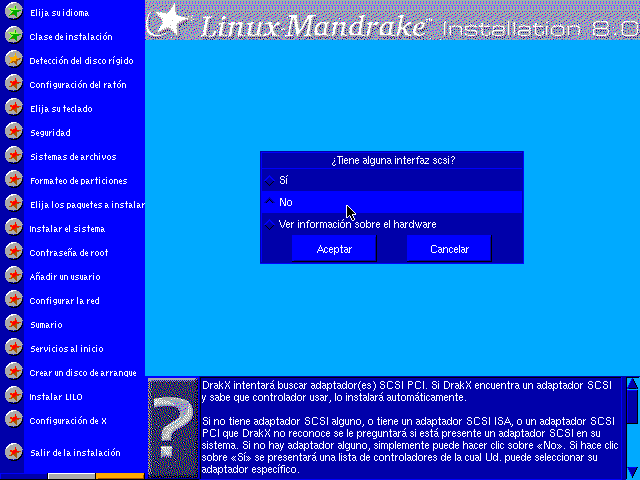
\includegraphics{dd/scsi.eps} \par}
\end{center}
\caption{SCSI Data Structures}
\label{scsi-figure}
\end{figure}
Now that every SCSI host has been discovered, the SCSI subsystem must find out what SCSI devices are
attached to each host's bus.
SCSI devices are numbered between 0 and 7 inclusively, each device's number or SCSI identifier  being
unique on the SCSI bus to which it is attached.
SCSI identifiers are usually set by jumpers on the device.
The SCSI initialization code finds each SCSI device on a SCSI bus by sending it a TEST\_UNIT\_READY command.
When a device responds, its identification is read by sending it an ENQUIRY command.
This gives Linux the vendor's name and the device's model and revision names.
SCSI commands are represented by a \ds{Scsi\_Cmnd} data structure and these are passed to the device driver
for this SCSI host by calling the device driver routines within its \ds{Scsi\_Host\_Template} data structure.
Every SCSI device that is found is represented by a \ds{Scsi\_Device} data structure, each of which points to
its parent \ds{Scsi\_Host}.
All of the \ds{Scsi\_Device} data structures are added to the \dsni{scsi\_devices}\index{scsi\_devices list} 
list.
Figure~\ref{scsi-figure} shows how the main data structures relate to one another.

There are four SCSI device types: disk, tape, CD and generic.
Each of these SCSI types are individually registered with the kernel as different major block device types.
However they will only register themselves if one or more of a given SCSI device type has been found.
Each SCSI type, for example SCSI disk,  maintains its own  tables of devices.
It uses these tables to direct kernel block operations (file or buffer cache) to the correct device
driver or SCSI host.
Each SCSI type is represented by a \ds{Scsi\_Device\_Template} data structure.
This contains information about this type of SCSI device and the addresses of routines to perform various
tasks.
The SCSI subsystem uses these templates to call the SCSI type routines for each type of SCSI device.
In other words, if the SCSI subsystem wishes to attach a SCSI disk device it will call the SCSI disk type
attach routine.
The \ds{Scsi\_Type\_Template} data structures are added to the \dsni{scsi\_devicelist}\index{scsi\_devicelist list}
list if one or more SCSI devices of that type have been detected.

The final phase of the SCSI subsystem initialization is to call the finish functions for each registered
\ds{Scsi\_Device\_Template}.
For the SCSI disk type this spins up all of the SCSI disks that were found and then records their disk geometry.
It also adds the \ds{gendisk} data structure representing all SCSI disks to the linked list of disks shown 
in Figure~\ref{gendisk-figure}.

\subsubsection{Delivering Block Device Requests}
Once Linux has initialized the SCSI subsystem, the SCSI devices may be used.
Each active SCSI device type registers itself with the kernel so that Linux can direct block
device requests to it.
There can be buffer cache requests via \dsni{blk\_dev}\index{blk\_dev vector} or file operations
via \dsni{blkdevs}\index{blkdevs vector}.
Taking a SCSI disk driver that has one or more EXT2 filesystem partitions as an example, how do kernel
buffer requests get directed to the right SCSI disk when one of its EXT2 partitions is mounted?

Each request to read or write a block of data to or from a SCSI disk partition results in a new
\ds{request} structure being added to the SCSI disks \dsni{current\_request} list in the \dsni{blk\_dev}
\index{blk\_dev vector} vector.
If the \ds{request} list is being processed, the buffer cache need not do anything else; otherwise
it must nudge the SCSI disk subsystem to go and process its request queue.
Each SCSI disk in the system is represented by a \ds{Scsi\_Disk} data structure.
These are kept in the \dsni{rscsi\_disks}\index{rscsi\_disks vector} vector that is indexed using
part of the SCSI disk partition's minor device number.
For exmaple, \fn{/dev/sdb1} has a major number of 8 and a minor number of 17; this generates an index of 1.
Each \ds{Scsi\_Disk} data structure contains a pointer to the \ds{Scsi\_Device} data structure representing
this device.
That in turn points at the \ds{Scsi\_Host} data structure which ``owns'' it.
The \ds{request} data structures from the buffer cache are translated into \ds{Scsi\_Cmd} structures describing
the SCSI command that needs to be sent to the SCSI device and this is queued onto the \ds{Scsi\_Host} 
structure representing this device.
These will be processed by the individual SCSI device driver once the appropriate data blocks have been
read or written.

\section{Network Devices}
\index{Network devices}
A network device is, so far as Linux's network subsystem is concerned, an entity that sends and receives
packets of data.
This is normally a physical device such as an ethernet card.
Some network devices though are software only such as the loopback device which is used for sending data to
yourself.
Each network device is represented by a \ds{device}\SeeModule{include/\-linux/\-netdevice.h} data structure.
Network device drivers register the devices that they control with Linux during network initialization
at kernel boot time.
The \ds{device} data structure contains information about the device and the addresses of functions that allow
the various supported network protocols to use the device's services.
These functions are mostly concerned with transmitting data using the network device.
The device uses standard networking support mechanisms to pass received data up to the appropriate protocol layer.
All network data (packets) transmitted and received are represented by \ds{sk\_buff} data structures, these are
flexible data structures that allow network protocol headers to be easily added and removed.
How the network protocol layers use the network devices, how they pass data back and forth using
\ds{sk\_buff} data structures is described in detail in the Networks chapter (Chapter~\ref{networks-chapter}).
This chapter concentrates on the \ds{device} data structure and on how network devices are discovered
and initialized.

The \ds{device} data structure contains information about the network device:
\begin{description}
	\item [Name] Unlike block and character devices which have their device special files created
		using the \eg{mknod} command, network device special files appear spontaniously as the
		system's network devices are discovered and initialized.
		Their names are standard, each name representing the type of device that it is.
		Multiple devices of the same type are numbered upwards from 0.  Thus the ethernet
		devices are known as \fn{/dev/eth0},\fn{/dev/eth1},\fn{/dev/eth2} and so on.  Some common network
		devices are:

		\begin{tabular}{ll}
		/dev/ethN   	&	Ethernet devices 	\\
		/dev/slN	&	SLIP devices 		\\
		/dev/pppN	&	PPP devices		\\
		/dev/lo 	&	Loopback devices	\\
		\end{tabular}
	\item [Bus Information] This is information that the device driver needs in order to control
		the device.   The {\em irq} number is the interrupt that this device is using.
		The {\em base address} is the address of any of the device's control and status registers
		in I/O memory.  The {\em DMA channel} is the DMA channel number that this network device is using.
		All of this information is set at boot time as the device is initialized.

	\item [Interface Flags] These describe the characteristics and abilities of the network device:

		\begin{tabular}{ll}
		IFF\_UP			&	Interface is up and running,				\\
		IFF\_BROADCAST		&	Broadcast address in \ds{device} is valid		\\
		IFF\_DEBUG		&	Device debugging turned on				\\
		IFF\_LOOPBACK		&	This is a loopback device				\\
		IFF\_POINTTOPOINT	&	This is point to point link (SLIP and PPP)		\\
		IFF\_NOTRAILERS		&	No network trailers 					\\
		IFF\_RUNNING		&	Resources allocated					\\
		IFF\_NOARP		& 	Does not support ARP protocol				\\
		IFF\_PROMISC		&	Device in promiscuous receive mode, it will receive 	\\
					&	all packets no matter who they are addressed to		\\
		IFF\_ALLMULTI		&	Receive all IP multicast frames				\\
		IFF\_MULTICAST		&	Can receive IP multicast frames				\\
		\end{tabular}
	\item [Protocol Information] Each device describes how it may be used by the network protocool layers:
		\begin{description}
			\item [mtu] The size of the largest packet that this network can transmit not including any
				link layer headers that it needs to add.   This maximum is used by the protocol layers,
				for example IP, to select suitable packet sizes to send.
			\item [Family] The family indicates the protocol family that the device can support.	The
				family for all Linux network devices is AF\_INET, the Internet address family.
			\item [Type] The hardware interface type describes the media that this network device is
				attached to.  There are many different types of media that Linux network devices
				support.  These include Ethernet, X.25, Token Ring, Slip, PPP and Apple Localtalk.
			\item [Addresses] The \ds{device} data structure holds a number of addresses that are relevent
				to this network device, including its IP addresses.
		\end{description}
	\item [Packet Queue] This is the queue of \ds{sk\_buff} packets queued waiting to be transmitted on
		this network device,
	\item [Support Functions] Each device provides a standard set of routines that protocol layers
		call as part of their interface to this device's link layer.   These include setup and
		frame transmit routines as well as routines to add standard frame headers and collect
		statistics.  These statistics can be seen using the \eg{ifconfig} command.
\end{description}

\subsection{Initializing Network Devices}
\index{Initializing Network devices}
\index{Network devices, initializing}
Network device drivers can, like other Linux device drivers, be built into the Linux kernel.
Each potential network device is represented by a \ds{device} data structure within the 
network device list pointed at by \dsni{dev\_base}\index{dev\_base list pointer} list pointer.
The network layers call one of a number of network device service routines whose addresses
are held in the \ds{device} data structure if they need device specific work performing.
Initially though, each \ds{device} data structure holds only the address of an initialization or probe
routine.

There are two problems to be solved for network device drivers.
Firstly, not all of the network device drivers built into the Linux kernel will have devices to control.
Secondly, the ethernet devices in the system are always called \fn{/dev/eth0}, \fn{/dev/eth1} and so on, no
matter what their underlying device drivers are.
The problem of ``missing'' network devices is easily solved.
As the initialization routine for each network device is called, it returns a status indicating 
whether or not it located an instance of the controller that it is driving.
If the driver could not find any devices, its entry in the \ds{device} list pointed at by 
\dsni{dev\_base}\index{dev\_base list pointer} is removed.
If the driver could find a device it fills out the rest of the \ds{device} data structure with information
about the device and the addresses of the support functions within the network device driver.

The second problem, that of dynamically assigning ethernet devices to the standard \fn{/dev/ethN} device
special files is solved more elegantly.
There are eight standard entries in the devices list; one for \fn{eth0}, \fn{eth1} and so on to
\fn{eth7}.
The initialization routine is the same for all of them, it tries each ethernet device driver built into
the kernel in turn until one finds a device.
When the driver finds its ethernet device it fills out the \fn{ethN} \ds{device} data structure,
 which it now owns.
It is also at this time that the network device driver initializes the physical hardware that it
is controlling and works out which IRQ it is using, which DMA channel (if any) and so on.
A driver may find several instances of the network device that it is controlling and, in this case, it will take
over several of the \fn{/dev/ethN} \ds{device} data structures.
Once all eight standard \fn{/dev/ethN} have been allocated, no more ethernet devices will be probed for.



\chapter{El sistema de archivos}
\label{filesystem-chapter}

\ChapterDescription{Este capitulo describe c�mo el kernel de Linux
  gestiona los ficheros en los sistemas de ficheros soportados por
  �ste.  Describe el Sistema de Ficheros Virtual (VFS) y explica c�mo
  los sistemas de ficheros reales del kernel de Linux son soportados.}

\index{File system} Una de los rasgos m�s importantes de Linux es su
soporte para diferentes sistemas de ficheros.  �sto lo hace muy
flexible y bien capacitado para coexistir con muchos otros sistemas
operativos.  En el momento de escribir �sto, Linux soporta 15 sistemas
de ficheros; \texttt{ext}, \texttt{ext2}, \texttt{xia},
\texttt{minix}, \texttt{umsdos}, \texttt{msdos}, \texttt{vfat},
\texttt{proc}, \texttt{smb}, \texttt{ncp}, \texttt{iso9660},
\texttt{sysv}, \texttt{hpfs}, \texttt{affs} and \texttt{ufs}, y sin
duda, con el tiempo se a�adir�n m�s.

En Linux, como en Unix\tm, a los distintos sistemas de ficheros que el
sistema puede usar no se accede por identificadores de dispositivo
(como un n�mero o nombre de unidad) pero, en cambio se combinan en una
simple structura jer�rquica de �rbol que representa el sistema de
ficheros como una entidad �nica y sencilla.  Linux a�ade cada sistema
de ficheros nuevo en este simple �rbol de sistemas de ficheros cuando
se monta.  Todos los sistemas de ficheros, de cualquier tipo, se
montan sobre un directorio y los ficheros del sistema de ficheros son
el contenido de ese directorio.  Este directorio se conoce como
directorio de montaje o punto de montaje.  Cuando el sistema de
ficheros se desmonta, los ficheros propios del directorio de montaje
son visibles de nuevo.

Cuando se inicializan los discos (usando \eg{fdisk}, por ejemplo)
tienen una estructura de partici�n inpuesta que divide el disco f�sico
en un n�mero de particiones l�gicas.  Cada partici�n puede mantener un
sistema de ficheros, por ejemplo un sistema de ficheros \texttt{EXT2}.
Los sistemas de ficheros organizan los ficheros en structuras
jer�rquicas l�gicas con directorios, enlaces flexibles y m�s
contenidos en los bloques de los dispositivos f�sicos.  Los
dispositivos que pueden contener sistemas de ficheros se conocen con
el nombre de dispositivos de bloque.  La partici�n de disco IDE
\fn{/dev/hda1}, la primera partici�n de la primera unidad de disco en
el sistema, es un dispositivo de bloque.  Los sistemas de ficheros de
Linux contemplan estos dispositivos de bloque como simples colecciones
lineales de bloques, ellos no saben o tienen en cuenta la geometr�a
del disco f�sico que hay debajo.  Es la tarea de cada controlador de
dispositivo de bloque asignar una petici�n de leer un bloque
particular de su dispositivo en t�rminos comprensibles para su
dispositivo; la pista en cuesti�n, sector y cilindro de su disco duro
donde se guarda el bloque.  Un sistema de ficheros tiene que mirar,
sentir y operar de la misma forma sin importarle con que dispositivo
est� tratando.  Por otra parte, al usar los sistemas de ficheros de
Linux, no importa (al menos para el usuario del sistema) que estos
distintos sistemas de ficheros est�n en diferentes soportes
controlados por diferentes controladores de hardware.  El sistema de
ficheros puede incluso no estar en el sistema local, puede ser
perfectamente un disco remoto montado sobre un enlace de red.
Considerese el siguiente ejemplo donde un sistema Linux tiene su
sistema de ficheros ra�z en un disco SCSI:
\begin{verbatim}
A         E         boot      etc       lib       opt       tmp       usr
C         F         cdrom     fd        proc      root      var       sbin
D         bin       dev       home      mnt       lost+found
\end{verbatim}
Ni los usuarios ni los programas que operan con los ficheros necesitan
saber que \fn{/C} de hecho es un sistema de ficheros VFAT montado que
est� en el primer disco IDE del sistema.  En el ejemplo (que es mi
sistema Linux en casa), \fn{/E} es el disco IDE primario en la segunda
controladora IDE.  No importa que la primera controladora IDE sea una
controladora PCI y que la segunda sea una controladora ISA que tambi�n
controla el IDE CDROM.  Puedo conectarme a la red donde trabajo usando
un modem y el protocolo de red PPP y en este caso puedo remotamente
montar mis sistemas de ficheros Linux \axp\ sobre \fn{/mnt/remote}.

Los ficheros en un sistema de ficheros son grupos de datos; el fichero
que contiene las fuentes de este cap�tulo es un fichero ASCII llamado
\fn{filesystems.tex}.  Un sistema de ficheros no s�lo posee los datos
contenidos dentro de los ficheros del sistema de ficheros, adem�s
mantiene la estructura del sistema de ficheros.  Mantiene toda la
informaci�n que los usuarios de Linux y procesos ven como ficheros,
directorios, enlaces flexibles, informaci�n de protecci�n de ficheros
y as�.  Por otro lado debe mantener esa informaci�n de forma eficiente
y segura, la integridad b�sica del sistema operativo depende de su
sistema de ficheros.  Nadie usaria un sistema operativo que perdiera
datos y ficheros de forma aleatoria\footnote{Bueno, no con
  conocimiento, sin embargo me he topado con sistemas operativos con
  m�s abogados que programadores tiene Linux}.

\texttt{Minix}, el primer sistema de ficheros que Linux tuvo es
bastante restrictivo y no era muy r�pido.  \texttt{Minix}, the first
file system that Linux had is rather restrictive and lacking in
performance.\index{Minix} Sus nombres de ficheros no pueden tener m�s
de 14 caracteres (que es mejor que nombres de ficheros 8.3) y el
tama�o m�ximo de ficheros es 64 MBytes.  64 MBytes puede a primera
vista ser suficiente pero se necesitan tama�os de ficheros m�s grandes
para soportar incluso modestas bases de datos.  El primer sistema de
ficheros dise�ado especificamente para Linux, el sistema de Ficheros
Extendido, o \texttt{EXT}, fue introducido en Abril de 1992 y solvent�
muchos problemas pero era aun falto de rapidez.  \index{EXT}
\index{Extended File system} As�, en 1993, el Segundo sistema de
Ficheros Extendido, o \texttt{EXT2}, fue a�adido.  \index{EXT2}
\index{Second Extended File system} Este es el sistema de ficheros que
se describe en detalle m�s tarde en este cap�tulo.

Un importante desarrollo tuvo lugar cuando se a�adi� en sistema de
ficheros EXT en Linux.  El sistema de ficheros real se separ� del
sistema operativo y servicios del sistema a favor de un interfaz
conocido como el sistema de Ficheros Virtual, o VFS.  \index{VFS}
\index{Virtual File system} VFS permite a Linux soportar muchos,
incluso muy diferentes, sistemas de ficheros, cada uno presentando un
interfaz software com�n al VFS.  Todos los detalles del sistema de
ficheros de Linux son traducidos mediante software de forma que todo
el sistema de ficheros parece id�ntico al resto del kernel de Linux y
a los programas que se ejecutan en el sistema.  La capa del sistema de
Ficheros Virtual de Linux permite al usuario montar de forma
transparente diferentes sistemas de ficheros al mismo tiempo.

El sistema de Ficheros Virtual est� implementado de forma que el
acceso a los ficheros es r�pida y tan eficiente como es posible.
Tambi�n debe asegurar que los ficheros y los datos que contiene son
correctos.  Estos dos requisitos pueden ser incompatibles uno con el
otro.  El VFS de Linux mantiene una antememoria con informaci�n de
cada sistema de ficheros montado y en uso.  Se debe tener mucho
cuidado al actualizar correctamente el sistema de ficheros ya que los
datos contenidos en las antememorias se modifican cuando cuando se
crean, escriben y borran ficheros y directorios.  Si se pudieran ver
las estructuras de datos del sistema de ficheros dentro del kernel en
ejecuci�n, se podria ver los bloques de datos que se leen y escriben
por el sistema de ficheros.  Las estructuras de datos, que describen
los ficheros y directorios que son accedidos serian creadas y
destruidas y todo el tiempo los controladores de los dispositivo
estarian trabajando, buascando y guardando datos.  La antememoria o
cach� m�s importantes es el Buffer Cache, que est� integrado entre
cada sistema de ficheros y su dispositivo de bloque.  Tal y como se
accede a los bloques se ponen en el Buffer Cache y se almacenan en
varias colas dependiendo de sus estados.  El Buffer Cache no s�lo
mantiene buffers de datos, tambien ayuda a administrar el interfaz
as�ncrono con los controladores de dispositivos de bloque.

\section{The Second Extended File system (EXT2)}
\index{EXT2}
\begin{figure}
\begin{center}
{\centering \includegraphics{fs/ext2.eps} \par}
\end{center}
\caption{Physical Layout of the EXT2 File system}
\label{ext2fs-figure}
\end{figure}
El Segundo sistema de ficheros Extendido fue pensado (por R�my Card)
como un sistema de ficheros extensible y poderoso para Linux.  Tambi�n
es el sistema de ficheros m�s �xito tiene en la comunidad Linux y es
b�sico para todas las distribuciones actuales de Linux.
\SeeModule{fs/�ext2/�*} El sistema de ficheros EXT2, como muchos
sistemas de ficheros, se construye con la premisa de que los datos
contenidos en los ficheros se guarden en bloques de datos.  Estos
bloques de datos son todos de la misma longitud y, si bien esa
longitud puede variar entre diferentes sistemas de ficheros EXT2 el
tama�o de los bloques de un sistema de ficheros EXT2 en particular se
decide cuando se crea (usando \eg{mke2fs}).  El tama�o de cada fichero
se redondea hasta un numero entero de bloques.  Si el tama�o de bloque
es 1024 bytes, entonces un fichero de 1025 bytes ocupar� dos bloques
de 1024 bytes.  Desafortunadamente esto significa que en promedio se
desperdicia un bloque por fichero.
Normalmente en ordenadores se cambia la carga de CPU por m�s espacio de memoria o de disco utilizado. En este caso Linux, como muchos sistemas operativos, cambia una ineficiencia relativa en el uso del disco a cambio de reducir la carga de la CPU.

No todos los bloques del sistema de ficheros contienen datos, algunos
deben usarse para mantener la informaci�n que describe la estructura
del sistema de ficheros.  EXT2 define la topologia del sistema de
ficheros describiendo cada fichero del sistema con una estructura de
datos inodo.  Un inodo describe que bloques ocupan los datos de un
fichero y tambi�n los permisos de acceso del fichero, las horas de
modificaci�n del fichero y el tipo del fichero.  Cada fichero en el
sistema de ficheros EXT2 se describe por un �nico inodo y cada inodo
tiene un �nico n�mero que lo identifica.  Los inodos del sistema de
ficheros se almacenan juntos en tablas de inodos.  Los directorios
EXT2 son simplemente ficheros especiales (ellos mismos descritos por
inodos) que contienen punteros a los inodos de sus entradas de
directorio.

La figura�\ref{ext2fs-figure} muestra la disposici�n del sistema de
ficheros EXT2 ocupando una serie de bloques en un dispositivo
estructurado bloque.  Por la parte que le toca a cada sistema de
ficheros, los dispositivos de bloque son s�lo una serie de bloques que
se pueden leer y escribir.  Un sistema de ficheros no se debe
preocupar donde se debe poner un bloque en el medio f�sico, eso es
trabajo del controlador del dispositivo.  Siempre que un sistema de
ficheros necesita leer informaci�n o datos del dispositivo de bloque
que los contiene, pide que su controlador de dispositivo lea un n�mero
entero de bloques.  El sistema de ficheros EXT2 divide las particiones
l�gicas que ocupa en Grupos de Bloque (Block Groups).  \index{EXT2
  Block Groups} Cada grupo duplica informaci�n cr�tica para la
integridad del sistema de ficheros ya sea valiendose de ficheros y
directorios como de bloques de informaci�n y datos.  Esta duplicaci�n
es necesaria por si ocurriera un desastre y el sistema de ficheros
necesitara recuperarse.  Los subapartados describen con m�s detalle
los contenidos de cada Grupo de Bloque.

\subsection{El inodo de EXT2}
\begin{figure}
\begin{center}
{\centering \includegraphics{fs/ext2_inode.eps} \par}
\end{center}
\caption{El inodo de EXT2}
\label{ext2fs-inode-figure}
\end{figure}
\index{El inodo de EXT2} \index{Estructuras de datos, el inodo EXT2} En el sistema de ficheros \texttt{EXT2}, el inodo es el bloque de construcci�n
b�sico; cada fichero y directorio del sistema de ficheros es descrito
por un y s�lo un inodo.  Los inodos EXT2 para cada Grupo de Bloque se
almacenan juntos en la table de inodos con un mapa de bits que permite
al sistema seguir la pista de inodos reservados y libres.  La
figura�\ref{ext2fs-inode-figure} muestra el formato de un inodo EXT2,
entre otra informaci�n, contiene los siguientes campos:
\SeeModule{include/\-linux/\-ext2\_fs\_i.h}
\begin{description}
\item [mode] Esto mantiene dos partes de informaci�n; qu� inodo
  describe y los permisos que tienen los usuarios.  Para EXT2, un
  inodo puede describir un ficheros, directorio, enlace simb�lico,
  dispositivo de bloque, dispositivo de caracter o FIFO.
\item [Owner Information] Los identificadores de usuario y grupo de
  los due�os de este fichero o directorio.  Esto permite al sistema de
  ficheros aplicar correctamente el tipo de acceso,
\item [Size] El tama�o en del fichero en bytes,
\item [Timestamps] La hora en la que el inodo fue creado y la �ltima
  hora en que se modific�,
\item [Datablocks] Punteros a los bloques que contienen los datos que
  este inodo describe.  Los doce primeros son punteros a los bloques
  f�sicos que contienen los datos descritos por este inodo y los tres
  �ltimos punteros contienen m�s y m�s niveles de indirecci�n.  Por
  ejemplo, el puntero de doble indirecci�n apunta a un bloque de
  punteros que apuntan a bloques de punteros que apuntan a bloques de
  datos.  Esto significa que ficheros menores o iguales a doce bloques
  de datos en longitud son m�s facilmente accedidos que ficheros m�s
  grandes.
\end{description}
Indicar que los inodos EXT2 pueden describir ficheros de dispositivo
especiales.  No son ficheros reales pero permiten que los programas
puedan usarlos para acceder a los dispositivos.  Todos los ficheros de
dispositivo de \fn{/dev} est�n ahi para permitir a los programas
acceder a los dispositivos de Linux.  Por ejemplo el programa
\eg{mount} toma como argumento el fichero de dispositivo que el
usuario desee montar.

\subsection{El superbloque EXT2}
\index{Superbloque EXT2} El Superbloque contiene una descripci�n del
tama�o y forma base del sistema de ficheros.  La informaci�n contenida
permite al administrador del sistema de ficheros usar y mantener el
sistema de ficheros.  Normalmente s�lo se lee el Superbloque del Grupo
de Bloque 0 cuando se monta el sistema de ficheros pero cada Grupo de
Bloque contiene una copia duplicada en caso de que se corrompa sistema
de ficheros.  Entre otra informaci�n contiene el:
\SeeModule{include/\-linux/\-ext2\_fs\_sb.h}
\begin{description}
\item [Magic Number] Esto permite al software de montaje comprobar que
  es realmente el Superbloque para un sistema de ficheros EXT2.  Para
  la versi�n actual de \texttt{EXT2} �ste es \hex{EF53}.
\item [Revision Level] Los niveles de revisi�n mayor y menor permiten
  al c�digo de montaje determinar si este sistema de ficheros soporta
  o no caracter�sticas que s�lo son disponibles para revisiones
  particulares del sistema de ficheros.  Tambi�n hay campos de
  compatibilidad que ayudan al c�digo de montaje determinar que nuevas
  caracter�sticas se pueden usar con seguridad en ese sistema de
  ficheros,
\item [Mount Count and Maximum Mount Count] Juntos permiten al sistema
  determinar si el sistema de ficheros fue comprobado correctamente.
  El contador de montaje se incrementa cada vez que se monta el
  sistema de ficheros y cuando es igual al contador m�ximo de montaje
  muestra el mensaje de aviso �maximal mount count reached, running
  e2fsck is recommended�,
\item [Block Group Number] El n�mero del Grupo de Bloque que tiene la
  copia de este Superbloque,
\item [Block Size] El tama�{o} de bloque para este sistema deficheros
  en bytes, por ejemplo 1024 bytes,
\item [Blocks per Group] El n�mero de bloques en un grupo.  Como el
  tama�o de bloque �ste se fija cuando se crea el sitema de ficheros,
\item [Free Blocks] EL n�mero de bloques libres en el sistema de
  ficheros,
\item [Free Inodes] El n�mero de Inodos libres en el sistema de
  ficheros,
\item [First Inode] Este es el n�mero de inodo del primer inodo en el
  sistema de ficheros.  El primer inodo en un sistema de ficheros EXT2
  ra�z seria la entrada directorio para el directorio '/'.
\end{description}

\subsection{The EXT2 Group Descriptor}
\index{EXT2 Group Descriptor} Cada Grupo de Bloque tiene una
estructura de datos que lo describe.  Como el Superbloque, todos los
descriptores de grupo para todos los Grupos de Bloque se duplican en
cada Grupo de Bloque en caso de corrupci�n del sistema de fichero.
\SeeCode{ext2\_group\_desc}{include/\-linux/\-ext2\_fs.h} Cada
Descriptor de Grupo contiene la siguiente informaci�n:
\begin{description}
\item [Blocks Bitmap] El n�mero de bloque del mapa de bits de bloques
  reservados para este Grupo de Bloque.  Se usa durante la reseva y
  liberaci�n de bloques,
\item [Inode Bitmap] El n�mero de bloque del mapa de bits de inodos
  reservados para este Grupo de Bloques.  Se usa durante la reserva y
  liberaci�n de inodos,
\item [Inode Table] El n�mero de bloque del bloque inicial para la
  tabla de inodos de este Grupo de Bloque.  Cada inodo se representa
  por la estructura de datos inodo EXT2 descrita abajo.
        \item [Free blocks count, Free Inodes count, Used directory count]
\end{description}
Los descriptores de grupo se colocan uno detr�s de otro y juntos hacen
la tabla de descriptor de grupo.  Cada Grupo de Bloques contiene la
tabla entera de descriptores de grupo despues de su copia del
Superbloque.  S�lo la primera copia (en Grupo de Bloque 0) es usada
por el sistema de ficheros EXT2.  Las otras copias est�n ahi, como las
copias del Superbloque, en caso de que se corrompa la principal.

\subsection{EXT2 Directories}
\index{EXT2 Directories}
\index{Data structures, EXT2 Directory}
\begin{figure}
\begin{center}
{\centering \includegraphics{fs/ext2_dir.eps} \par}
\end{center}
\caption{EXT2 Directory}
\label{ext2fs-dir-figure}
\end{figure}
En el sistema de ficheros EXT2, los directorios son ficheros
especiales que se usan para crear y mantener rutas de acceso a los
ficheros en el sistema de ficheros.  La figura�\ref{ext2fs-dir-figure}
muestra la estructura de una estrada directorio en memoria.
\SeeCode{ext2\_dir\_entry}{include/\-linux/\-ext2\_fs.h} Un fichero
directorio es una lista de entradas directorio, cada una conteniendo
la siguiente informaci�n:
\begin{description}
\item [inode] El inodo para esta entrada directorio.  Es un �ndice al
  vector de inodos guardada en la Tabla de Inodos del Grupo de Bloque.
  En la figura�\ref{ext2fs-dir-figure}, la entrada directorio para el
  fichero llamado \fn{file} tiene una referencia al n�mero de inodo
  \texttt{i1},
\item [name length] La longitud de esta entrada directorio en bytes,
        \item [name] El nombre de esta entrada directorio.
\end{description}
Las dos primeras entradas para cada directorio son siempre las
entradas estandar �.� y �..� significando �este directorio� y �el
directorio padre� respectivamente.

\subsection{Finding a File in an EXT2 File System}
Un nombre de fichero Linux tiene el mismo formato que los nombres de
ficheros de todos los Unix\tm\.  Es una serie de nombres de
directorios separados por contra barras (�\fn{/}�) y acabando con el
nombre del fichero.  Un ejemplo de nombre de fichero podria ser
\fn{/home/rusling/.cshrc} donde \fn{/home} y \fn{/rusling} son nombres
de directorio y el nombre del fichero es \fn{.cshrc}.  Como todos los
demas sistemas Unix\tm� Linux no tiene encuenta el formato del nombre
del fichero; puede ser de cualquier longitud y cualquier caracter
imprimible.  Para encontrar el inodo que representa a este fichero
dentro de un sistema de ficheros \texttt{EXT2} el sistema debe
analizar el nombre del fichero directorio a directorio hasta encontrar
el fichero en si.  El primer inodo que se necesita es el inodo de la
ra�z del sistema de ficheros, que est� en el superbloque del sistema
de ficheros.  Para leer un inodo EXT2 hay que buscarlo en la tabla de
inodos del Grupo de Bloque apropiado.  Si, por ejemplo, el n�mero de
inodo de la ra�z es 42, entonces necesita el inodo 42avo de la tabla
de inodos del Grupo de Bloque 0.  El inodo ra�z es para un directorio
EXT2, en otras palabras el modo del inodo lo describe como un
directorio y sus bloques de datos contienen entradas directorio EXT2.

\fn{home} es una de las muchas entradas directorio y esta entrada
directorio indica el n�mero del inodo que describe al directorio
\fn{/home}.  Hay que leer este directorio (primero leyendo su inodo y
luego las entradas directorio de los bloques de datos descritos por su
inodo) para encontrar la entrada \fn{rusling} que indica el numero del
inodo que describe al directorio \fn{/home/rusling}.  Finalmente se
debe leer las entradas directorio apuntadas por el inodo que describe
al directorio \fn{/home/rusling} para encontrar el n�mero de inodo del
fichero \fn{.cshrc} y desde ahi leer los bloques de datos que
contienen la informaci�n del fichero.

\subsection{Changing the Size of a File in an EXT2 File System}
Un problema com�n de un sistema de ficheros es la tendencia a
fragmentarse.  Los bloques que contienen los datos del fichero se
esparcen por todo el sistema de ficheros y esto hace que los accesos
secuenciales a los bloques de datos de un fichero sean cada vez m�s
ineficientes cuanto m�s alejados est�n los bloques de datos.  El
sistema de ficheros EXT2 intenta solucionar esto reservando los nuevos
bloques para un fichero, fisicamente juntos a sus bloques de datos
actuales o al menos en el mismo Grupo de Bloque que sus bloques de
datos.  S�lo cuando esto falla, reserva bloques de datos en otros
Grupos de Bloque.

Siempre que un proceso intenta escribir datos a un fichero, el sistema
de ficheros Linux comprueba si los datos exceden el final del �ltimo
bloque para el fichero.  Si lo hace, entonces tiene que reservar un
nuevo bloque de datos para el fichero.  Hasta que la reserva no haya
acabado, el proceso no puede ejecutarse; debe esperarse a que el
sistema de ficheros reserve el nuevo bloque de datos y escriba el
resto de los datos antes de continuar.  La primera cosa que hacen las
rutinas de reserva de bloques EXT2 es bloquear el Superbloque EXT2 de
ese sistema de ficheros.  La reserva y liberaci�n cambia campos del
superbloque, y el sistema de ficheros Linux no puede permitir m�s de
un proceso haciendo �sto a la vez.  Si otro proceso necesita reservar
m�s bloques de datos, debe esperarse hasta que el otro proceso acabe.
Los procesos que esperan el superbloque son suspendidos, no se pueden
ejecutar, hasta que el control del superbloque lo abandone su usuario
actual.  El acceso al superbloque se garantiza mediante una pol�tica
�el primero que llega se atiende primero�, y cuando un proceso tiene
control sobre el superbloque le pone cerrojo hasta que no lo necesita
m�s. \footnote{REVISAR!!!} bloqueado el superbloque, el proceso
comprueba que hay suficientes bloques libres en ese sistema de
ficheros.  Si no es as�, el intento de reservar m�s bloques falla y el
proceso ceder� el control del superbloque del sistema de ficheros.

Si hay suficientes bloques en el sistema de ficheros, el proceso
intenta reservar uno.
\SeeCode{ext2\_new\_block()}{fs/\-ext2/\-balloc.c} Si el sistema de
ficheros EXT2 se ha compilado para prereservar bloques de datos
entonces se podr� usar uno de estos.  La prereserva de bloques no
existe realmente, s�lo se reservan dentro del mapa de bits de bloques
reservados.  El inodo VFS que representa el fichero que intenta
reservar un nuevo bloque de datos tiene dos campos EXT2 espec�ficos,
\field{prealloc\_block} y \field{prealloc\_count}, que son el numero
de bloque del primer bloque de datos prereservado y cuantos hay,
respectivamente.  Si no habian bloques prereservados o la reserva
anticipada no est� activa, el sistema de ficheros EXT2 debe reservar
un nuevo bloque.  El sistema de ficheros EXT2 primero mira si el
bloque de datos despues del �ltimo bloque de datos del fichero est�
libre.  Logicamente, este es el bloque m�s eficiente para reservar ya
que hace el acceso secuencial mucho m�s r�pido.  Si este bloque no
est� libre, la b�squeda se ensancha y busca un bloque de datos dentro
de los 64 bloques del bloque ideal.  Este bloque, aunque no sea ideal
est� al menos muy cerca y dentro del mismo Grupo de Bloque que los
otros bloques de datos que pertenecen a ese fichero.

Si incluso ese bloque no est� libre, el proceso empieza a buscar en
los dem�s Grupos de Bloque hasta encontrar algunos bloques libres.  El
c�digo de reserva de bloque busca un cluster de ocho bloques de datos
libres en cualquiera de los Grupos de Bloque.  Si no puede encontrar
ocho juntos, se ajustar� para menos.  Si se quiere la prereserva de
bloques y est� activado, actualizar� \field{prealloc\_block} y
\field{prealloc\_count} pertinentemente.

Donde quiera que encuentre el bloque libre, el c�digo de reserva de
bloque actualiza el mapa de bits de bloque del Grupo de Bloque y
reserva un buffer de datos en el buffer cach�.  Ese buffer de datos se
identifica unequivocamente por el identificador de dispositivo del
sistema y el n�mero de bloque del bloque reservado.  El buffer de
datos se sobreescribe con ceros y se marca como �sucio� para indicar
que su contenido no se ha escrito al disco f�sico.  Finalmente, el
superbloque se marca como �sucio� para indicar que se ha cambiado y
est� desbloqueado.  Si hubiera otros procesos esperando, al primero de
la cola se le permitiria continuar la ejecuci�n y terner el control
exclusido del superbloque para sus operaciones de fichero.  Los datos
del proceso se escriben en el nuevo bloque de datos y, si ese bloque
se llena, se repite el proceso entero y se reserva otro bloque de
datos.

\section{The Virtual File System (VFS)}
\index{Virtual File System (VFS)}
\index{VFS}
\begin{figure}
\begin{center}
{\centering \includegraphics{fs/vfs.eps} \par}
\end{center}
\caption{A Logical Diagram of the Virtual File System}
\label{vfs-figure}
\end{figure}
La figura�\ref{vfs-figure} muestra la relaci�n entre el Sistema de
Ficheros Virtual del kernel de Linux y su sistema de ficheros real.
El sistema de ficheros vitual debe mantener todos los diferentes
sistemas de ficheros que hay montados en cualquier momento.  Para
hacer esto mantiene unas estructuras de datos que describen el sistema
de ficheros (virtual) por entero y el sistema de ficheros, montado,
real.  \SeeModule{fs/*} De forma m�s confusa, el VFS describe los
ficheros del sistema en t�rminos de superbloque e inodos de la misma
forma que los ficheros EXT2 usan superbloques e inodos.  Como los
inodos EXT2, los inodos VFS describen ficheros y directorios dentro
del sistema; los contenidos y topolog�a del Sistema de Ficheros
Virtual.  De ahora en adelante, para evitar confusiones, se escribir�
inodos CFS y superbloques VFS para distinguirlos de los inodos y
superbloques EXT2.

Cuando un sistema de ficheros se inicializa, se registra �l mismo con
el VFS.  Esto ocurre cuando el sistema operativo se inicializa en el
momento de arranque del sistema.  Los sistemas de ficheros reales
est�n compilados con el nucleo o como m�dulos cargables.  Los m�dulos
de Sistemas de Ficheros se cargan cuando el sistema los necesita, as�,
por ejemplo, si el sistema de ficheros \texttt{VFAT} est� implementado
como m�dulo del kernel, entonces s�lo se carga cuando se monta un
sistema de ficheros \texttt{VFAT}.  Cuando un dispositivo de bloque
base se monta, y �ste incluye el sistema de ficheros ra�z, el VFS debe
leer su superbloque.  Cada rutina de lectura de superbloque de cada
tipo de sistema de ficheros debe resolver la topolog�a del sistema de
ficheros y mapear esa informaci�n dentro de la estructura de datos del
superbloque VFS.  El VFA mantiene una lista de los sitema de ficheros
montados del sistema junto con sus superbloques VFS.  Cada superbloque
VFS contiene informaci�n y punteros a rutinas que realizan funciones
particulares.  De esta forma, por ejemplo, el superbloque que
representa un sistema de ficheros EXT2 montado contiene un puntero a
la rutina de lectura de inodos espec�fica.  Esta rutina, como todas
las rutinas de lectura de inodos del sistema de ficheros espe�fico,
rellena los campos de un inodo VFS.  Cada superbloque VFS contiene un
puntero al primer inodo VFS del sistema de ficheros.  Para el sistema
de ficheros ra�z, �ste es el inodo que representa el directorio
\fn{�/�}.  Este mapeo de informaci�n es muy eficiente para el sistema
de ficheros EXT2 pero moderadamente menos para otros sistema de
ficheros.

Ya que los procesos del sistema acceden a directorios y ficheros, las
rutinas del sistema se dice que recorren los inodos VFS del sistema.
\SeeModule{fs/�inode.c} Por ejemplo, escribir \eg{ls} en un directorio
o \eg{cat} para un fichero hacen que el Sistema de Ficheros Virtual
busque atrav�s de los inodos VFS que representan el sistema de
ficheros.  Como cada fichero y directorio del sistema se representa
por un inodo VFS, un n�mero de inodos ser�n accedidos repetidamente.
Estos inodos se mantienen en la antememoria, o cach�, de inodos que
hace el acceso mucho m�s r�pido.  Si un inodo no est� en la cach�,
entonces se llama a una rutina espec�fica del sistema de ficheros para
leer el inodo apropiado.  La acci�n de leer el inodo hace que se ponga
en la cach� de inodos y siguientes accesos hacen que se mantenga en la
cach�.  Los inodos VFS menos usados se quitan de la cach�.

Todos los sistemas de ficheros de Linux usan un buffer cach� com�n
para mantener datos de los dispositivos para ayudar a acelerar el
acceso por todos los sistemas de ficheros al dispositivo f�sico que
contiene los sistemas de ficheros.  \SeeModule{fs/�buffer.c} Este
buffer cach� es independiente del sistema de ficheros y se integra
dentro de los mecanismos que el n�cleo de Linux usa para reservar,
leer y escribir datos.  Esto tiene la ventaja de hacer los sistemas de
ficheros de Linux independientes del medio y de los controladores de
dispositivos que los soportan.  Tofos los dispositivos estructurados
de bloque se registran ellos mismos con el n�cleo de Linux y presentan
una interfaz uniforme, basada en bloque y normalmente as�ncrona.
Incluso dispositivos de bloque relativamente complejos como SCSI lo
hacen.

Cuando el sistema de ficheros real lee datos del disco f�sico realiza
una petici�n al controlador de dispositivo de bloque para leer los
bloques f�sicos del dispositivo que controla.  Integrado en este
interfaz de dispositivo de bloque est� el buffer cach�.  Al leer
bloques del sistema de ficheros se guardan en un el buffer cach�
global compartido por todos los sistemas de ficheros y el n�cleo de
Linux.  Los buffers que hay dentro se identifican por su n�mero de
bloque y un identificador �nico para el dispositivo que lo ha leido.
De este modo, si se necesitan muy a menudo los mismos datos, se
obtendr�n del buffer cach� en lugar de leerlos del disco, que tarda
m�s tiempo.  Algunos dispositivos pueden realizar lecturas anticipadas
(\textit{read ahead}), mediante lo cual se realizan lecturas antes de
necesitarlas, especulando con que se utilizar�n m�s
adelante.\footnote{REVISAR!!!!!} 

El VFS tambi�n mantiene una cach� de directorios donde se pueden
encontrar los inodos de los directorios que se usan de forma m�s
frecuente.  \SeeModule{fs/�dcache.c} Como experimento, probar a listar
un directorio al que no se haya accedido recientemente.  La primera
vez que se lista, se puede notar un peque�o retardo pero la segunda
vez el resultado es inmediato.  El cach� directorio no almacena
realmente los inodos de los directorios; �stos estar�n en el cach� de
inodos, el directorio cach� simplemente almacena el mapa entre el
nombre entero del directorio y sus n�meros de inodo.

\subsection{The VFS Superblock}
\index{Superblock, VFS} \index{VFS superblock} Cada sistema de
ficheros montado est� representado por un superbloque VFS; entre otra
informaci�n, el superbloque VFS contiene:
\SeeModule{include/�linux/�fs.h}
\begin{description}
\item [Device] Es el identificador de dispositivo para el dispositivo
  bloque que contiene este a este sistema de ficheros.  Por ejemplo,
  \fn{/dev/hda1}, el primer disco duro IDE del sistema tiene el
  identificador de dispositivo \hex{301},
\item [Inode pointers] El puntero de inodo \field{montado} apunta al
  primer inodo del sistema de ficheros.  El puntero de inodo
  \field{cubierto} apunta al inodo que representa el directorio donde
  est� montado el sistema de ficheros.  El superbloque VFS del sistema
  de ficheros ra�z no tiene puntero \field{cubierto},
\item [Blocksize] EL tama�o de bloque en bytes del sistema de
  ficheros, por ejemplo 1024 bytes,
\item [Superblock operations] Un puntero a un conjunto de rutinas de
  superbloque para ese sistema de ficheros.  Entre otras cosas, estas
  rutinas las usa el VFS para leer y escribir inodos y superbloques.
\item [File System type] Un puntero a la estructura de datos
  \ds{tipo\_sistema\_ficheros} del sistema de ficheros montado,
\item [File System specific] Un puntero a la informaci�n que necesaria
  este sistema de ficheros.
\end{description}

\subsection{The VFS Inode}
\index{inode, VFS} \index{VFS inode} Como el sistema de ficheros EXT2,
cada fichero, directorio y dem�s en el VFS se representa por uno y
solo un inodos VFS.  \SeeModule{include/�linux/�fs.h} La infomaci�n en
cada inodo VFS se construye a partir de informaci�n del sistema de
ficheros por las rutinas espec�ficas del sistema de ficheros.  Los
inodos VFS existen s�lo en la memoria del n�cleo y se mantienen en el
cach� de inodos VFS tanto tiempo como sean �tiles para el sistema.
Entre otra informaci�n, los inodos VFS contienen los siguientes
campos:
\begin{description}
\item [device] Este es el identificador de dispositivo del dispositivo
  que contiene el fichero o lo que este inodo VFS represente,
\item [inode number] Este es el n�mero del inodo y es �nico en este
  sistema de ficheros.  La combinaci�n de \field{device} y
  \field{inode number} es �nica dentro del Sistema de Ficheros
  Virtual,
\item [mode] Como en EXT2 este campo describe que representa este
  inodo VFS y sus permisos de acceso,
\item [user ids] Los identificadores de propietario,
\item [times] Los tiempos de creaci�n, modificaci�n y escritura,
\item [block size] El tama�o de bloque en bytes para este fichero, por
  ejemplo 1024 bytes,
\item [inode operations] Un puntero a un bloque de direcciones de
  rutina.  Estas rutinas son espef�ficas del sistema de ficheros y
  realizan operaciones para este inodo, por ejemplo, truncar el
  fichero que representa este inodo.
\item [count] El n�mero de componentes del sistema que est�n usando
  actualmente este inodo VFS.  Un contador de cero indica que el inodo
  est� libre para ser descartado o reusado,
\item [lock] Este campo se usa para bloquear el inodo VFS, por
  ejemplo, cuando se lee del sistema de ficheros,
\item [dirty] Indica si se ha escrito en este inodo, si es as�{i} el
  sistema de ficheros necesitar� modificarlo,
\item [file system specific information]
\end{description}

\subsection{Registering the File Systems}
\begin{figure}
\begin{center}
{\centering \includegraphics{fs/file-systems.eps} \par}
\end{center}
\caption{Registered File Systems}
\label{file-systems-figure}
\end{figure}
\index{File System, registering} \index{Registering a file system}
Cuando se compila el n�cleo de Linux se pregunta si se quiere cada uno
de los sistemas de ficheros soportados.  Cuando el n�cleo est�
compilado, el c�difo de arranque del sistema de ficheros contiene
llamadas a las rutinas de inicializaci�n de todos los sistemas de
ficheros compilados.  \SeeCode{sys\_setup()}{fs/\-filesystems.c} Los
sistemas de ficheros de Linux tambi�n se pueden compilar como m�dulos
y, en este caso, pueden ser cargados cuando se les necesita o
cargarlos a mano usando \eg{insmod}.  Siempre que un m�dulo de sistema
de ficheros se carga se registra �l mismo con el n�cleo y se borra �l
mismo cuando se descarga.  Cada rutina de inicializaci�n del sistema
de ficheros se registra con el Sistema de Ficheros Virtual y se
representa por una estructura de datos \ds{tipo\_sistema\_ficheros}
que contiene el nombre del sistema de ficheros y un puntero a su
rutina de lectura de superbloque VFS.  La
figura�\ref{file-systems-figure} muestra que las estructuras de datos
\ds{tipo\_sistems\_ficheros} se ponen en una lista apuntada por el
puntero \ds{sistemas\_ficheros}.  Cada estructura de datos
\ds{tipo\_sistema\_ficheros} contiene la siguiente informaci�n:
\SeeCode{file\_system\_type}{include/\-linux/\-fs.h}
\begin{description}
\item [Superblock read routine] Esta rutina se llama por el VFS cuando
  se monta una instancia del sistema de ficheros,
\item [File System name] El nombre de este sistema de ficheros, por
  ejemplo \texttt{ext2},
\item [Device needed] Necesita soportar este sistema de ficheros un
  dispositivo?  No todos los sistemas de ficheros necesitan un
  dispositivo.  El sistema de fichero \texttt{/proc}, por ejemplo, no
  requiere un dispositivo de bloque,
\end{description}
Se puede ver que sistemas de ficheros hay rgistrados mirando en
\fn{/proc/filesystems}.  Por ejemplo:
\begin{verbatim}
      ext2
nodev proc
      iso9660
\end{verbatim}

\subsection{Mounting a File System}
\index{Mounting a File System} \index{File System, mounting} Cuando el
superusuario intenta montar un sistema de ficheros, el n�cleo de Linux
debe primero validar los argumentos pasados en la llamada al sistema.
Aunque \eg{mount} hace una comprobaci�n b�sica, no conoce que sistemas
de ficheros soporta el kernel o si existe el punto de montaje
propuesto.  Considerar el siguiente comando \eg{mount}:
\begin{verbatim}
$ mount -t iso9660 -o ro /dev/cdrom /mnt/cdrom
\end{verbatim}% $ para que no moleste el modo AUC-TeX de Emacs
Este comando \eg{mount} pasa al n�cleo tres trozos de informaci�n; el
nombre del sistema de ficheros, el dispositivo de bloque f�sico que
contiene al sistema de fichros y, por �ltimo, donde, en la topolog�a
del sistema de ficheros existente, se montar� el nuevo sistema de
ficheros.

La primera cosa que debe hacer el Sistema de Ficheros Virtual es
encontrar el sistema de ficheros.  \SeeCode{do\_mount()}{fs/\-super.c}
Para hacer �{es}to busca a trav�s de la lista de sistemas de ficheros
conocidos y mira cada estructura de datos ds{tipo\_sistema\_ficheros}
en la lista apuntada por \ds{sistema\_ficheros}.
\SeeCode{get\_fs\_type()}{fs/\-super.c} Si encuentra una coincidencia
del nombre ahora sabe que ese tipo de sistema de ficheros es soportado
por el n�cleo y tiene la direcci�n de la rutina espec�fica del sistema
de ficheros para leer el superbloque de ese sistema de ficheros.  Si
no puede encontrar ninguna coindidencia no todo est� perdido si el
n�cleo puede cargar m�dulos por demanda (ver
Cap�tulo�\ref{modules-chapter}).  En este caso el n�cleo piede al
demonio del n�cleo que cargue el m�dulo del sistema de ficheros
apropiado antes de continuar como anteriormente.

Si el dispositivo f�sico pasado por \eg{mount} no est� ya montado,
debe encontrar el inodo VFS del directorio que ser� el punto de
montaje del nuevo sistema de ficheros.  Este inodo VFS debe estar en
el cach� de inodos o se debe leer del dispositivo de bloque que
soporta el sistema de ficheros del punto de montaje.  Una vez que el
inodo se ha encontrado se comprueba para ver que sea un directorio y
que no contenga ya otro sistema de ficheros montado.  El mismo
directorio no se puede usar como punto de montaje para m�s de un
sistema de ficheros.

En este punto el c�difo de montaje VFS reserva un superbloque VFS y le
pasa la informaci�n de montahe a la rutina de lectura de superblque
para este sistema de ficheros.  Todos los superbloques VFS del sistema
se mantienen en el vector \ds{super\_bloques} de las estructuras de
datos \ds{super\_bloque} y se debe reservar una para este montaje.  La
rutina de lectura de superbloque debe rellenar los campos b�sicos del
superbloque VFS con informaci�n que lee del dispositivo f�sico.  Para
el sistema de ficheros EXT2 este mapeo o traducci�n de informaci�n es
bastante facil, simplemente lee el superbloque EXT2 y rellena el
superbloque VFS de ah�.  Para otros sistemas de ficheros, como el MS
DOS, no es una tarea t�n facil.  Cualquiera que sea el sistema de
ficheros, rellenar el superbloque VFS significa que el sistema de
ficheros debe leer todo lo que lo describe del dispositivo de bloque
que lo soporta.  Si el dispositivo de bloque no se puede leer o si no
contiene este tipo de sistema de ficheros entonces el comando
\eg{mount} fallar�.

\begin{figure}
\begin{center}
{\centering \includegraphics{fs/mounted.eps} \par}
\end{center}
\caption{A Mounted File System}
\label{mounted-figure}
\end{figure}
Cada sistema de ficheros montado es descrito por una estructura de
datos \ds{vfsmount}; ver figura�\ref{mounted-figure}.  Estos son
puestos en una cola de una lista apuntada por \ds{vfsmntlist}.
\SeeCode{add\_vfsmnt()}{fs/�super.c} Otro puntero, \ds{vfsmnttail}
apunta a la �ltima entrada de la lista y el puntero
\dsni{mru\_vfsmnt}\index{mru\_vfsmnt pointer} apunta al sistemas de
ficheros m�s recientemente usado.  Cada estructura \ds{vfsmount}
contiene el n�mero de dispositivo del dispositivo de bloque que
contiene al sistema de ficheros, el directorio donde el sistema de
ficheros est� montado y un puntero al superbloque VFS reservado cuando
se mont�.  En cambio el superbloque VFS apunta a la estructura de
datos \ds{tipo\_sistema\_ficheros} para este tipo de sisetma de
ficheros y al inodo ra�{i}z del sistema de ficheros.  Este inodo se
mantiene residente en el cach� de inodos VFS todo el tiempo que el
sistema de ficheros est� cargado.

\subsection{Finding a File in the Virtual File System}
\index{Finding a File} \index{Files, finding} Para encontrar el inodo
VFS de un fichero en el Sistema de Ficheros Virtual, VFS debe resolver
el nombre del directorio, mirando el inodo VFS que representa cada uno
de los directorios intermedios del nombre.  Mirar cada directorio
envuelve una llamada al sistema de ficheros espec�fico cuya direcci�n
se mantiene en el inodo VFS que representa al directorio padre.  Esto
funciona porque siempre tenemos el inodo VFS del ra�z de cada sistema
de ficheros disponible y apuntado por el superbloque VFS de ese
sistema.  Cada vez que el sistema de ficheros real mira un inodo
comprueba el cach� de directorios.  Si no est� la entrada en el cach�
de directorios, el sistema de ficheros real toma el inodo VFS tanto
del sistema de ficheros como del cach� de inodos.

\subsection{Creating a File in the Virtual File System}
\index{Creating a file}
\index{Files, creating}

\subsection{Unmounting a File System}
\index{Unmounting a File System} \index{File System, unmounting} The
workshop manual for my MG usually describes assembly as the reverse of
disassembly and the reverse is more or less true for unmounting a file
system.  \SeeCode{do\_umount()}{fs/�super.c} A file system cannot be
unmounted if something in the system is using one of its files.  So,
for example, you cannot umount \fn{/mnt/cdrom} if a process is using
that directory or any of its children.  If anything is using the file
system to be unmounted there may be VFS inodes from it in the VFS
inode cache, and the code checks for this by looking through the list
of inodes looking for inodes owned by the device that this file system
occupies.  If the VFS superblock for the mounted file system is dirty,
that is it has been modified, then it must be written back to the file
system on disk.  Once it has been written to disk, the memory occupied
by the VFS superblock is returned to the kernel's free pool of memory.
Finally the \ds{vfsmount} data structure for this mount is unlinked
from \ds{vfsmntlist} and freed.
\SeeCode{remove\_vfsmnt()}{fs/�super.c}

\subsection{The VFS Inode Cache}
\index{Inode cache} \index{Caches, VFS inode} As the mounted file
systems are navigated, their VFS inodes are being continually read
and, in some cases, written.  The Virtual File System maintains an
inode cache to speed up accesses to all of the mounted file systems.
Every time a VFS inode is read from the inode cache the system saves
an access to a physical device.  \SeeModule{fs/�inode.c}

The VFS inode cache is implmented as a hash table whose entries are
pointers to lists of VFS inodes that have the same hash value.  The
hash value of an inode is calculated from its inode number and from
the device identifier for the underlying physical device containing
the file system.  Whenever the Virtual File System needs to access an
inode, it first looks in the VFS inode cache.  To find an inode in the
cache, the system first calculates its hash value and then uses it as
an index into the inode hash table.  This gives it a pointer to a list
of inodes with the same hash value.  It then reads each inode in turn
until it finds one with both the same inode number and the same device
identifier as the one that it is searching for.

If it can find the inode in the cache, its count is incremented to
show that it has another user and the file system access continues.
Otherwise a free VFS inode must be found so that the file system can
read the inode from memory.  VFS has a number of choices about how to
get a free inode.  If the system may allocate more VFS inodes then
this is what it does; it allocates kernel pages and breaks them up
into new, free, inodes and puts them into the inode list.  All of the
system's VFS inodes are in a list pointed at by \ds{first\_inode} as
well as in the inode hash table.  If the system already has all of the
inodes that it is allowed to have, it must find an inode that is a
good candidate to be reused.  Good candidates are inodes with a usage
count of zero; this indicates that the system is not currently using
them.  Really important VFS inodes, for example the root inodes of
file systems always have a usage count greater than zero and so are
never candidates for reuse.  Once a candidate for reuse has been
located it is cleaned up.  The VFS inode might be dirty and in this
case it needs to be written back to the file system or it might be
locked and in this case the system must wait for it to be unlocked
before continuing.  The candidate VFS inode must be cleaned up before
it can be reused.

However the new VFS inode is found, a file system specific routine
must be called to fill it out from information read from the
underlying real file system.  Whilst it is being filled out, the new
VFS inode has a usage count of one and is locked so that nothing else
accesses it until it contains valid information.

To get the VFS inode that is actually needed, the file system may need
to access several other inodes.  This happens when you read a
directory; only the inode for the final directory is needed but the
inodes for the intermediate directories must also be read.  As the VFS
inode cache is used and filled up, the less used inodes will be
discarded and the more used inodes will remain in the cache.

\subsection{The Directory Cache}
\index{Directory cache} \index{Caches, directory} To speed up accesses
to commonly used directories, the VFS maintains a cache of directory
entries.  \SeeModule{fs/�dcache.c} As directories are looked up by the
real file systems their details are added into the directory cache.
The next time the same directory is looked up, for example to list it
or open a file within it, then it will be found in the directory
cache.  Only short directory entries (up to 15 characters long) are
cached but this is reasonable as the shorter directory names are the
most commonly used ones.  For example, \fn{/usr/X11R6/bin} is very
commonly accessed when the X server is running.

The directory cache consists of a hash table, each entry of which
points at a list of directory cache entries that have the same hash
value.  The hash function uses the device number of the device holding
the file system and the directory's name to calculate the offset, or
index, into the hash table.  It allows cached directory entries to be
quickly found.  It is no use having a cache when lookups within the
cache take too long to find entries, or even not to find them.

In an effort to keep the caches valid and up to date the VFS keeps
lists of Least Recently Used (LRU) directory cache entries.  When a
directory entry is first put into the cache, which is when it is first
looked up, it is added onto the end of the first level LRU list.  In a
full cache this will displace an existing entry from the front of the
LRU list.  As the directory entry is accessed again it is promoted to
the back of the second LRU cache list.  Again, this may displace a
cached level two directory entry at the front of the level two LRU
cache list.  This displacing of entries at the front of the level one
and level two LRU lists is fine.  The only reason that entries are at
the front of the lists is that they have not been recently accessed.
If they had, they would be nearer the back of the lists.  The entries
in the second level LRU cache list are safer than entries in the level
one LRU cache list.  This is the intention as these entries have not
only been looked up but also they have been repeatedly referenced.

\ReviewNotes{Do we need a diagram for this?}

\section{The Buffer Cache}
\index{Buffer caches}
\index{Caches, buffer}
\begin{figure}
\begin{center}
{\centering \includegraphics{fs/buffer-cache.eps} \par}
\end{center}
\caption{The Buffer Cache}
\label{buffer-cache-figure}
\end{figure}
As the mounted file systems are used they generate a lot of requests
to the block devices to read and write data blocks.  All block data
read and write requests are given to the device drivers in the form of
\ds{buffer\_head} data structures via standard kernel routine calls.
These give all of the information that the block device drivers need;
the device identifier uniquely identifies the device and the block
number tells the driver which block to read.  All block devices are
viewed as linear collections of blocks of the same size.  To speed up
access to the physical block devices, Linux maintains a cache of block
buffers.  All of the block buffers in the system are kept somewhere in
this buffer cache, even the new, unused buffers.  This cache is shared
between all of the physical block devices; at any one time there are
many block buffers in the cache, belonging to any one of the system's
block devices and often in many different states.  If valid data is
available from the buffer cache this saves the system an access to a
physical device.  Any block buffer that has been used to read data
from a block device or to write data to it goes into the buffer cache.
Over time it may be removed from the cache to make way for a more
deserving buffer or it may remain in the cache as it is frequently
accessed.

Block buffers within the cache are uniquely identfied by the owning
device identifier and the block number of the buffer.  The buffer
cache is composed of two functional parts.  The first part is the
lists of free block buffers.  There is one list per supported buffer
size and the system's free block buffers are queued onto these lists
when they are first created or when they have been discarded.  The
currently supported buffer sizes are 512, 1024, 2048, 4096 and 8192
bytes.  The second functional part is the cache itself.  This is a
hash table which is a vector of pointers to chains of buffers that
have the same hash index.  The hash index is generated from the owning
device identifier and the block number of the data block.
Figure�\ref{buffer-cache-figure} shows the hash table together with a
few entries.  Block buffers are either in one of the free lists or
they are in the buffer cache.  When they are in the buffer cache they
are also queued onto Least Recently Used (LRU) lists.  There is an LRU
list for each buffer type and these are used by the system to perform
work on buffers of a type, for example, writing buffers with new data
in them out to disk.  The buffer's type reflects its state and Linux
currently supports the following types:
\begin{description}
\item [clean] Unused, new buffers,
\item [locked] Buffers that are locked, waiting to be written,
\item [dirty] Dirty buffers.  These contain new, valid data, and will
  be written but so far have not been scheduled to write,
\item [shared] Shared buffers,
\item [unshared] Buffers that were once shared but which are now not
  shared,
\end{description}

Whenever a file system needs to read a buffer from its underlying
physical device, it trys to get a block from the buffer cache.  If it
cannot get a buffer from the buffer cache, then it will get a clean
one from the appropriate sized free list and this new buffer will go
into the buffer cache.  If the buffer that it needed is in the buffer
cache, then it may or may not be up to date.  If it is not up to date
or if it is a new block buffer, the file system must request that the
device driver read the appropriate block of data from the disk.

Like all caches, the buffer cache must be maintained so that it runs
efficiently and fairly allocates cache entries between the block
devices using the buffer cache.  Linux uses the \texttt{bdflush}
\index{bdflush, kernel daemon} \index{Kernel daemons, bdflush} kernel
daemon to perform a lot of housekeeping duties on the cache but some
happen automatically as a result of the cache being used.

\subsection{The \texttt{bdflush} Kernel Daemon}
\index{bdflush, kernel daemon} \index{Kernel daemons, bdflush}
\SeeCode{bdflush()}{fs/�buffer.c} The \texttt{bdflush} kernel daemon
is a simple kernel daemon that provides a dynamic response to the
system having too many dirty buffers; buffers that contain data that
must be written out to disk at some time.  It is started as a kernel
thread at system startup time and, rather confusingly, it calls itself
�kflushd� and that is the name that you will see if you use the
\eg{ps} command to show the processes in the system.  Mostly this
daemon sleeps waiting for the number of dirty buffers in the system to
grow too large.  As buffers are allocated and discarded the number of
dirty buffers in the system is checked.  If there are too many as a
percentage of the total number of buffers in the system then
\texttt{bdflush} is woken up.
The default threshold is 60% but, if the system is desperate for buffers, \texttt{bdflush}
will be woken up anyway.
This value can be seen and changed using the \eg{update} command:
\begin{verbatim}

# update -d

bdflush version 1.4
0:    60 Max fraction of LRU list to examine for dirty blocks
1:   500 Max number of dirty blocks to write each time bdflush activated
2:    64 Num of clean buffers to be loaded onto free list by refill_freelist
3:   256 Dirty block threshold for activating bdflush in refill_freelist
4:    15 Percentage of cache to scan for free clusters
5:  3000 Time for data buffers to age before flushing
6:   500 Time for non-data (dir, bitmap, etc) buffers to age before flushing
7:  1884 Time buffer cache load average constant
8:     2 LAV ratio (used to determine threshold for buffer fratricide).

\end{verbatim}
All of the dirty buffers are linked into the \texttt{BUF\_DIRTY} LRU
list whenever they are made dirty by having data written to them and
\texttt{bdflush} tries to write a reasonable number of them out to
their owning disks.  Again this number can be seen and controlled by
the \eg{update} command and the default is 500 (see above).

\subsection{The \eg{update} Process}
\index{update process} The \eg{update} command is more than just a
command; it is also a daemon.  When run as superuser (during system
initialisation) it will periodically flush all of the older dirty
buffers out to disk.  It does this by calling a system service routine
\SeeCode{sys\_bdflush()}{fs/�buffer.c} that does more or less the same
thing as \texttt{bdflush}.  Whenever a dirty buffer is finished with,
it is tagged with the system time that it should be written out to its
owning disk.  Every time that \eg{update} runs it looks at all of the
dirty buffers in the system looking for ones with an expired flush
time.  Every expired buffer is written out to disk.

\section{The /proc File System}
\index{/proc file system} The \texttt{/proc} file system really shows
the power of the Linux Virtual File System.  It does not really exist
(yet another of Linux's conjuring tricks), neither the \texttt{/proc}
directory nor its subdirectories and its files actually exist.  So how
can you \eg{cat} \fn{/proc/devices}?  The {/proc} file system, like a
real file system, registers itself with the Virtual File System.
However, when the VFS makes calls to it requesting inodes as its files
and directories are opened, the \texttt{/proc} file system creates
those files and directories from information within the kernel.  For
example, the kernel's \fn{/proc/devices} file is generated from the
kernel's data structures describing its devices.

The \texttt{/proc} file system presents a user readable window into
the kernel's inner workings.  Several Linux subsystems, such as Linux
kernel modules described in chapter�\ref{modules-chapter}, create
entries in the the \texttt{/proc} file system.

\section{Ficheros especiales de dispostivo}
\index{Device Special Files} Linux, like all versions of Unix\tm\ 
presents its hardware devices as special files.  So, for example,
/dev/null is the null device.  A device file does not use any data
space in the file system, it is only an access point to the device
driver.  The EXT2 file system and the Linux VFS both implement device
files as special types of inode.  There are two types of device file;
character and block special files.  Within the kernel itself, the
device drivers implement file semantices: you can open them, close
them and so on.  Character devices allow I/O operations in character
mode and block devices require that all I/O is via the buffer cache.
When an I/O request is made to a device file, it is forwarded to the
appropriate device driver within the system.  Often this is not a real
device driver but a pseudo-device driver for some subsystem such as
the SCSI device driver layer.  Device files are referenced by a major
number, which identifies the device type, and a minor type, which
identifies the unit, or instance of that major type.  For example, the
IDE disks on the first IDE controller in the system have a major
number of 3 and the first partition of an IDE disk would have a minor
number of 1.  So, \texttt{ls -l}\index{ls command} of \fn{/dev/hda1}
gives: \marginnote{see \fn{/include/linux/\\major.h} for all of
  Linux's major device numbers.}
\begin{verbatim}
$ brw-rw----   1 root    disk       3,    1  Nov 24  15:09 /dev/hda1
\end{verbatim}
Within the kernel, every device is uniquely described by a
\dsni{kdev\_t}\index{kdev\_t data type} data type, this is two bytes
long, the first byte containing the minor device number and the second
byte holding the major device number.
\SeeModule{include/�linux/�kdev\_t.h} The IDE device above is held
within the kernel as \hex{0301}.  An EXT2 inode that represents a
block or character device keeps the device's major and minor numbers
in its first direct block pointer.  When it is read by the VFS, the
VFS inode data structure representing it has its \field{i\_rdev} field
set to the correct device identifier.

\chapter{Networks}
\label{networks-chapter}
\label{network-chapter}
\ChapterDescription{Networking and Linux are terms that are almost synonymous.
In a very real sense Linux is a product of the Internet or World Wide Web (WWW).
Its developers and users use the web to exchange information ideas, code, and Linux itself
is often used to support the networking needs of organizations.
This chapter describes how Linux supports the network protocols known collectively as
TCP/IP.}

The TCP/IP protocols were designed to support communications between computers connected to the
ARPANET, an American research network funded by the US government.
The ARPANET pioneered networking concepts such as packet switching and protocol layering
where one protocol uses the services of another.
ARPANET was retired in 1988 but its successors (NSF\footnote{National Science Foundation} NET and
the Internet) have grown even larger.
What is now known as the World Wide Web grew from the ARPANET and is itself supported by the
TCP/IP protocols.
Unix\tm\ was extensively used on the ARPANET and the first released networking version of 
Unix\tm\ was 4.3 BSD.
Linux's networking implementation is modeled on 4.3 BSD in that it supports BSD sockets (with
some extensions) and the full range of TCP/IP networking.
This programming interface was chosen because of its popularity and to help applications
be portable between Linux and other Unix\tm\ platforms.

\section{An Overview of TCP/IP Networking}
This section gives an overview of the main principles of TCP/IP networking.
It is not meant to be an exhaustive description, for that I suggest that you read
\cite[Comer]{bib-comer}.
 
In an IP network every machine is assigned an IP address,
this is a 32 bit number that uniquely identifies the machine.
The WWW is a very large, and growing, IP network and every machine that is connected to it has to have
a unique IP address assigned to it.
IP addresses are represented by four numbers separated by dots, for example, \fn{16.42.0.9}.
This IP address is actually in two parts, the {\em network} address and the {\em host} address.
The sizes of these parts may vary (there are several classes of IP addresses) 
but using \fn{16.42.0.9} as an example, the network address would
be \fn{16.42} and the host address \fn{0.9}.
The host address is further subdivided into a {\em subnetwork} and a {\em host} address.
Again, using \fn{16.42.0.9} as an example, the subnetwork address would be \fn{16.42.0} and the host
address {16.42.0.9}.
This subdivision of the IP address allows organizations to subdivide their networks.
For example, \fn{16.42} could be the network address of the ACME Computer Company; \fn{16.42.0} would
be subnet \fn{0} and \fn{16.42.1} would be subnet \fn{1}.
These subnets might be in separate buildings, perhaps connected by leased telephone lines or even
microwave links.
IP addresses are assigned by the network administrator and having IP subnetworks is a good way
of distributing the administration of the network.
IP subnet administrators are free to allocate IP addresses within their IP subnetworks.

Generally though, IP addresses are somewhat hard to remember.
Names are much easier.
\fn{linux.acme.com} is much easier to remember than \fn{16.42.0.9} but there must be some mechanism
to convert the network names into an IP address.
These names can be statically specified in the \fn{/etc/hosts} file or Linux can ask a Distributed Name Server (DNS
server) to resolve the name for it.
In this case the local host must know the IP address of one or more DNS servers and these are specified
in \fn{/etc/resolv.conf}.

Whenever you connect to another machine, say when reading a web page, its IP address is used to 
exchange data with that machine.
This data is contained in IP packets each of which have an IP header containing the 
IP addresses of the source and destination machine's IP addresses, a checksum and other useful information.
The checksum is derived from the data in the IP packet and allows the receiver of IP packets to tell if the
IP packet was corrupted during transmission, perhaps by a noisy telephone line.
The data transmitted by an application may have been broken down into smaller packets which are easier
to handle.
The size of the IP data packets varies depending on the connection media; ethernet packets are generally 
bigger than PPP packets.
The destination host must reassemble the data packets before giving the data to the receiving application.
You can see this fragmentation and reassembly of data graphically if you access a web page containing a lot of 
graphical images via a moderately slow serial link.

Hosts connected to the same IP subnet can send IP packets directly to each other, all other IP packets
will be sent to a special host, a gateway.  
Gateways (or routers) are connected to more than one IP subnet and they will resend IP packets
received on one subnet, but destined for another onwards.
For example, if subnets \fn{16.42.1.0} and \fn{16.42.0.0} are connected together by a gateway then
any packets sent from subnet \fn{0} to subnet \fn{1} would have to be directed to the gateway so that it
could route them.
The local host builds up routing tables which allow it to route IP packets to the correct machine.
For every IP destination there is an entry in the routing tables which tells Linux which host to send 
IP packets to in order that they reach their destination.
These routing tables are dynamic and change over time as applications use the network and as the network
topology changes.

\begin{figure}
\begin{center}
{\centering \includegraphics{net/protocols.eps} \par}
\end{center}
\caption{TCP/IP Protocol Layers}
\label{protocols-figure}
\end{figure}
The IP protocol is a transport layer that is used by other protocols to carry their data.
The Transmission Control Protocol (TCP) is a reliable end to end protocol that uses IP to transmit
and receive its own packets.
Just as IP packets have their own header, TCP has its own header.
TCP is a connection based protocol where two networking applications are connected by a single,
virtual connection even  though there may be many subnetworks, gateways and routers between
them.
TCP reliably transmits and receives data between the two applications and guarantees that there will
be no lost or duplicated data.  
When TCP transmits its packet using IP, the data contained within the IP packet is the TCP packet itself.
The IP layer on each communicating host is responsible for transmitting and receiving IP packets.
User Datagram Protocol (UDP) also uses the IP layer to transport its packets, unlike TCP, UDP is not
a reliable protocol but offers a datagram service.
This use of IP by other protocols means that when IP packets are received the receiving IP layer must 
know which upper protocol layer to give the data contained in this IP packet to.
To facilitate this every IP packet header has a byte containing a protocol identifier.
When TCP asks the IP layer to transmit an IP packet , that IP packet's header states that it contains
a TCP packet.
The receiving IP layer uses that protocol identifier to decide which layer to pass the received data
up to, in this case the TCP layer.
When applications communicate via TCP/IP they must specify not only the target's IP address but also the
{\em port} address of the application.
A port address uniquely identifies an application and standard network applications use standard port
addresses; for example, web servers use port 80.
These registered port addresses can be seen in \fn{/etc/services}.

This layering of protocols does not stop with TCP, UDP and IP.
The IP protocol layer itself uses many different physical media to transport IP packets to other
IP hosts.
These media may themselves add their own protocol headers.
One such example is the ethernet layer, but PPP and SLIP are others.
An ethernet network allows many hosts to be simultaneously connected to a single physical
cable.
Every transmitted ethernet frame can be seen by all connected hosts and so every ethernet
device has a unique address.
Any ethernet frame transmitted to that address will be received by the addressed host but
ignored by all the other hosts connected to the network.
These unique addresses are built into each ethernet device when they are manufactured and it
is usually kept in an SROM\footnote{Synchronous Read Only Memory} on the ethernet card.
Ethernet addresses are 6 bytes long, an example would be \fn{08-00-2b-00-49-A4}.
Some ethernet addresses are reserved for multicast purposes and ethernet frames sent with
these destination addresses will be received by all hosts on the network.
As ethernet frames can carry many different protocols (as data) they, like IP packets, 
contain a protocol identifier in their headers.
This allows the ethernet layer to correctly receive IP packets and to pass them onto the
IP layer.

In order to send an IP packet via a multi-connection protocol such as ethernet, the IP layer 
must find the ethernet address of the IP host.
This is because IP addresses are simply an addressing concept, the ethernet devices themselves
have their own physical addresses.
IP addresses on the other hand can be assigned and reassigned by network administrators at will 
but the network hardware responds only to ethernet frames with its own physical address or to special
multicast addresses which all machines must receive.
Linux uses the Address Resolution Protocol (or ARP) to allow machines to translate
IP addresses into real hardware addresses such as ethernet addresses.
A host wishing to know the hardware address associated with an IP address sends an ARP request packet
containing the IP address that it wishes translating to all nodes on the network by sending it to
a multicast address.
The target host that owns the IP address, responds with an ARP reply that contains its physical
hardware address.
ARP is not just restricted to ethernet devices, it can resolve IP addresses for other physical
media, for example FDDI.
Those network devices that cannot ARP are marked so that Linux does not attempt to ARP.
There is also the reverse function, Reverse ARP or RARP, which translates phsyical network
addresses into IP addresses.
This is used by gateways, which respond to ARP requests on behalf of IP addresses that are in the
remote network.

\section{The Linux TCP/IP Networking Layers}
\begin{figure}
\begin{center}
{\centering \includegraphics{net/layers.eps} \par}
\end{center}
\caption{Linux Networking Layers}
\label{layers-figure}
\end{figure}
Just like the network protocols themselves, 
Figure~\ref{layers-figure} shows that Linux implements the internet protocol address family
as a series of connected layers of software.
BSD sockets are supported by a generic socket management software concerned only with BSD sockets.
Supporting this is the INET socket layer, this 
manages the communication end points for the IP based protocols TCP and UDP.
UDP (User Datagram Protocol) is a connectionless protocol whereas TCP (Transmission Control Protocol) is a 
reliable end to end protocol.
When UDP packets are transmitted, Linux neither knows nor cares if they arrive safely at their destination.
TCP packets are numbered and both ends of the TCP connection make sure that transmitted data is received
correctly.
The IP layer contains code implementing the Internet Protocol.
This code prepends IP headers to transmitted data and understands how to route incoming IP packets to either
the TCP or UDP layers.
Underneath the IP layer, supporting all of Linux's networking are the network devices, for example PPP
and ethernet.
Network devices do not always represent physical devices; some like the loopback device are purely
software devices.
Unlike standard Linux devices that are created via the \eg{mknod}
command, network devices appear only if the underlying software has found and initialized them.
You will only see \fn{/dev/eth0} when you have built a kernel with the appropriate ethernet device driver 
in it.
The ARP protocol sits between the IP layer and the protocols that support ARPing for addresses.

\section{The BSD Socket Interface}
\index{BSD Sockets}
\index{Sockets, BSD}
This is a general interface which not only supports various forms of networking but is also an
inter-process communications mechanism.
A socket describes one end of a communications link, two communicating processes would each have
a socket describing their end of the communication link between them.
Sockets could be thought of as a special case of pipes but, unlike pipes, sockets have no limit
on the amount of data that they can contain.
Linux supports several classes of socket and these are known as {\em address families}.
This is because each class has its own method of addressing its communications.
Linux supports the following socket address families or domains:

\begin{tabular}{ll}
	UNIX		&	Unix domain sockets, \\
	INET		&	The Internet address family supports communications via \\
			&	TCP/IP protocols \\
	AX25		&	Amateur radio X25 \\
	IPX		&	Novell IPX \\
	APPLETALK	&	Appletalk DDP \\
	X25		&	X25 \\
\end{tabular}

There are several socket types and these represent the type of service that supports the connection.
Not all address families support all types of service.
Linux BSD sockets support a number of socket types:
\begin{description}
	\item [Stream] These sockets provide reliable two way sequenced data streams with a guarantee
		that data cannot be lost, corrupted or duplicated in transit.  Stream sockets are 
		supported by the TCP protocol of the Internet (INET) address family.
	\item [Datagram] These sockets also provide two way data transfer but, unlike stream sockets, 
		there is no guarantee that the messages will arrive.  Even if they do arrive there is
		no guarantee that they will arrive in order or even not be duplicated or corrupted.
		This type of socket is supported by the UDP protocol of the Internet address family.
	\item [Raw] This allows processes direct (hence ``raw'') access to the underlying protocols.
		It is, for example, possible to open a raw socket to an ethernet device and see
		raw IP data traffic.
	\item [Reliable Delivered Messages] These are very like datagram sockets but the data is
		guaranteed to arrive.
	\item [Sequenced Packets] These are like stream sockets except that the data packet sizes
		are fixed.
	\item [Packet] This is not a standard BSD socket type, it is a Linux specific extension that
		 allows processes to access packets directly at the device level.  
\end{description}

Processes that communicate using sockets use a client server model.
A server provides a service and clients make use of that service.
One example would be a Web Server, which provides web pages and a web client, or browser, which reads 
those pages.
A server using sockets, first creates a socket and then binds a name to it.
The format of this name is dependent on the socket's address family and it is, in effect, the local
address of the server.
The socket's name or address is specified using the \ds{sockaddr} data structure.
An INET socket would have an IP port address bound to it.
The registered port numbers can be seen in \fn{/etc/services}; for example, the port number for 
a web server is 80.
Having bound an address to the socket, the server then listens for incoming connection requests
specifying the bound address.
The originator of the request, the client, creates a socket and makes a connection request on it,
specifying the target address of the server.
For an INET socket the address of the server is its IP address and its port number.
These incoming requests must find their way up through the various protocol layers and then
wait on the server's listening socket.
Once the server has received the incoming request it either accepts or rejects it.
If the incoming request is to be accepted, the server must create a new socket to accept it 
on.
Once a socket has been used for listening for incoming connection requests it cannot be used
to support a connection.
With the connection established both ends are free to send and receive data.
Finally, when the connection is no longer needed it can be shutdown.
Care is taken to ensure that data packets in transit are correctly dealt with.

The exact meaning of operations on a BSD socket depends on its underlying address family.
Setting up TCP/IP connections is very different from setting up an amateur radio X.25 connection.
Like the virtual filesystem, Linux abstracts the socket interface with the BSD socket layer being 
concerned with the BSD socket interface to the application programs which is in turn supported by 
independent address family specific software.
At kernel initialization time, the address families built into the kernel register themselves with the 
BSD socket interface.
Later on, as applications create and use BSD sockets, an association is made between the BSD
socket and its supporting address family.
This association is made via cross-linking data structures and tables of address family specific
support routines.
For example there is an address family specific socket creation routine which the BSD socket
interface uses when an application creates a new socket.

When the kernel is configured, a number of address families and protocols are built into the \dsni{protocols}
\index{protocols vector} vector.
Each is represented by its name, for example ``INET'' and the address of its initialization routine.
When the socket interface is initialized at boot time each protocol's initialization routine is called.
For the socket address families this results in them registering a set of protocol operations.
This is a set of routines, each of which performs a a particular operation specific to that address
family.
The registered protocol operations are kept in the \dsni{pops}\index{pops vector} vector, a vector
of pointers to \ds{proto\_ops} data structures.
\SeeModule{include/\-linux/\-net.h}
The \ds{proto\_ops} data structure consists of the address family type and a set of pointers to socket
operation routines specific to a particular address family.
The \dsni{pops} vector is indexed by the address family identifier, for example the Internet address 
family identifier (AF\_INET is 2).

\begin{figure}
\begin{center}
{\centering \includegraphics{net/sockets.eps} \par}
\end{center}
\caption{Linux BSD Socket Data Structures}
\label{sockets-figure}
\end{figure}

\section{The INET Socket Layer}
\index{INET socket layer}
\index{Socket layer, INET}
The INET socket layer supports the internet address family which contains the TCP/IP protocols.
As discussed above, these protocols are layered, one protocol using the services of another.
Linux's TCP/IP code and data structures reflect this layering.
Its interface with the BSD socket layer is through the set of Internet address family socket operations
which it registers with the BSD socket layer during network initialization.
These are kept in the \dsni{pops}\index{pops vector} vector along with the other registered address
families.
The BSD socket layer calls the INET layer socket support routines from the registered INET \ds{proto\_ops}
data structure to perform work for it.
For example a BSD socket create request that gives the address family as INET will use the underlying
INET socket create function.
The BSD socket layer passes the \ds{socket} data structure representing the BSD socket to the INET layer
in each of these operations.
Rather than clutter the BSD \ds{socket} wiht TCP/IP specific information, the INET socket layer uses
its own data structure, the \ds{sock}\SeeModule{include/\-net/\-sock.h} which it links to the BSD \ds{socket}
data structure.
This linkage can be seen in Figure~\ref{sockets-figure}.
It links the \ds{sock} data structure to the BSD \ds{socket} data structure using the \dsni{data} pointer
in the BSD \ds{socket}.
This means that subsequent INET socket calls can easily retrieve the \ds{sock} data structure.
The \ds{sock} data structure's protocol operations pointer is also set up at creation time and it depends
on the  protocol requested.
If TCP is requested, then the \ds{sock} data structure's protocol operations pointer will point to
the set of TCP protocol operations needed for a TCP connection.

\subsection{Creating a BSD Socket}
\index{BSD Sockets, creating}
The system call to create a new socket passes identifiers for its address family, 
socket type and protocol.
\SeeCode{sys\_socket()}{net/\-socket.c}
Firstly the requested address family  is used to search the \dsni{pops} vector for a matching
address family.
It may be that a particular address family is implemented as a kernel module and, in this case,
the \texttt{kerneld} daemon must load the module before we can continue.
A new \ds{socket} data structure is allocated to represent the BSD socket.
Actually the \ds{socket} data structure is physically part of the VFS \ds{inode} data structure
and allocating a socket really means allocating a VFS \ds{inode}.
This may seem strange unless you consider that sockets can be operated on in just the same way
that ordinairy files can.
As all files are represented by a VFS \ds{inode} data structure, then in order to support file
operations, BSD sockets must also be represented by a VFS \ds{inode} data structure.

The newly created BSD \ds{socket} data structure contains a pointer to the address family
specific socket routines and this is set to the \ds{proto\_ops} data structure retrieved from
the \dsni{pops} vector.
Its type is set to the sccket type requested; one of SOCK\_STREAM, SOCK\_DGRAM and so on.
The address family specific creation routine is called using the address kept in the 
\ds{proto\_ops} data structure.

A free file descriptor is allocated from the current processes \dsni{fd}\index{fd vector} vector
and the \ds{file} data structure that it points at is initialized.
This includes setting the file operations pointer to point to the set of BSD socket file
operations supported by the BSD socket interface.
Any future operations will be directed to the socket interface
and it will in turn pass them to the supporting address family by calling its address family operation
routines.

\subsection{Binding an Address to an INET BSD Socket}
\index{Bind}
In order to be able to listen for incoming internet connection requests, each server must create an
INET BSD socket and bind its address to it.
The bind operation is mostly handled within the INET socket layer with some support from the
underlying TCP and UDP protocol layers.
The socket having an address bound to cannot be being used for any other communication.
This means that the \ds{socket}'s state must be \dsni{TCP\_CLOSE}.
The \ds{sockaddr} pass to the bind operation contains the IP address to be bound to and, optionally,
a port number.
Normally the IP address bound to would be one that has been assigned to a network device
that supports the INET address family and whose interface is up and able to be used.
You can see which network interfaces are currently active in the system by using the 
\eg{ifconfig} command.
The IP address may also be the IP broadcast address of either all 1's or all 0's.
These are special addresses that mean ``send to everybody''\footnote{duh?  What used for?}.
The IP address could also be specified as any IP address if the machine is acting as a transparent
proxy or firewall, but only processes with superuser privileges can bind to any IP address.
The IP address bound to is saved in the \ds{sock} data structure in the \dsni{recv\_addr} and
\dsni{saddr} fields.
These are used in hash lookups and as the sending IP address respectively.
The port number is optional and if it is not specified the supporting network
is asked for a free one.
By convention, port numbers less than 1024 cannot be used by processes without superuser privileges.
If the underlying network does allocate a port number it always allocates ones greater than
1024.

As packets are being received by the underlying network devices they must be routed to the correct
INET and BSD sockets so that they can be processed.
For this reason UDP and TCP maintain hash tables which are used to lookup the addresses 
within incoming IP messages and direct them to the correct \ds{socket}/\ds{sock} pair.
TCP is a connection oriented protocol and so there is more information involved in processing
TCP packets than there is in processing UDP packets.

UDP maintains a hash table of allocated UDP ports, the \dsni{udp\_hash}\index{upd\_hash table}
table.
This consists of pointers to \ds{sock} data structures indexed by a hash function based
on the port number.
As the UDP hash table is much smaller than the number of permissible port numbers 
(\dsni{udp\_hash}\index{upd\_hash table} is only 128 or \dsni{UDP\_HTABLE\_SIZE} entries long)
some entries in the table point to a chain of \ds{sock} data structures linked together using
each \ds{sock}'s \dsni{next} pointer.

TCP is much more complex as it maintains several hash tables.
However, TCP does not actually add the binding \ds{sock} data stucture into its hash tables
during the bind operation, it merely checks that the port number requested is not currently
being used.
The \ds{sock} data structure is added to TCP's hash tables during the {\em listen} operation.

\ReviewNotes{What about the route entered?}

\subsection{Making a Connection on an INET BSD Socket}
Once a socket has been created and, provided it has not been used to listen for inbound connection
requests, it can be used to make outbound connection requests.
For connectionless protocols like UDP this socket operation does not do a whole lot but for connection
orientated protocols like TCP it involves building a virtual circuit between two applications.

An outbound connection can only be made on an INET BSD socket that is in the right state; that is to say
one that  does not already have a connection established and one that is not being used for listening
for inbound connections.
This means that the BSD \ds{socket} data structure must be in state \dsni{SS\_UNCONNECTED}.
The UDP protocol does not establish virtual connections between applications, any messages sent
are datagrams, one off messages that may or may not reach their destinations.
It does, however, support the {\em connect} BSD socket operation.
A connection operation on a UDP INET BSD socket simply sets up the addresses of the remote application;
its IP address and its IP port number.
Additionally it sets up a cache of the routing table entry so that UDP packets sent on this BSD socket
do not need to check the routing database again (unless this route becomes invalid).
The cached routing information is pointed at from the \dsni{ip\_route\_cache} pointer in the 
INET \ds{sock} data structure.
If no addressing information is given, this cached routing and IP addressing information will be 
automatically be used for messages sent using this BSD socket.
UDP moves the \ds{sock}'s state to \dsni{TCP\_ESTABLISHED}.

For a connect operation on a TCP BSD socket, TCP must build a TCP message containing the connection
information and send it to IP destination given.
The TCP message contains information about the connection, a unique starting message sequence number,
the maximum sized message that can be managed by the initiating host, the transmit and receive window
size and so on.
Within TCP all messages are numbered and the initial sequence number is used as the first message
number.
Linux chooses a reasonably random value to avoid malicious protocol attacks.
Every message transmitted by one end of the TCP connection and successfully received by the other is 
acknowledged to say that it arrived successfully and uncorrupted.
Unacknowledges messages will be retransmitted.
The transmit and receive window size is the number of outstanding messages that there can be without an
acknowledgement being sent.
The maximum message size is based on the network device that is being used at the initiating end of the 
request.
If the receiving end's network device supports smaller maximum message sizes then the connection will 
use the minimum of the two.
The application making the outbound TCP connection request must now wait for a response from the 
target application to accept or reject the connection request.
As the TCP \ds{sock} is now expecting incoming messages, it is added to the \dsni{tcp\_listening\_hash}
so that incoming TCP messages can be directed to this \ds{sock} data structure.
TCP also starts timers so that the outbound connection request can be timed out if the target application
does not respond to the request.

\subsection{Listening on an INET BSD Socket}
Once a socket has had an address bound to it, it may listen for incoming connection 
requests specifying the bound addresses.
A network application can listen on a socket without first binding an address to it; in this
case the INET socket layer finds an unused port number (for this protocol) and automatically
binds it to the socket.
The listen socket function moves the socket into state \dsni{TCP\_LISTEN} and does any 
network specific work needed to allow incoming connections.

For UDP sockets, changing the socket's state is enough but TCP now adds the socket's
\ds{sock} data structure into two hash tables as it is now active.
These are the \dsni{tcp\_bound\_hash}\index{tcp\_bound\_hash table} table and the 
\dsni{tcp\_listening\_hash}\index{tcp\_listening\_hash table}.
Both are indexed via a hash function based on the IP port number.

Whenever an incoming TCP connection request is received for an active listening socket,
TCP builds a new \ds{sock} data structure to represent it.
This \ds{sock} data structure will become the bottom half of the TCP connection when it is
eventually accepted.
It also clones the incoming \ds{sk\_buff} containing the connection request and queues it onto
the \dsni{receive\_queue} for the listening \ds{sock} data structure.
The clone \ds{sk\_buff} contains a pointer to the newly created \ds{sock} data structure.

\subsection{Accepting Connection Requests}
UDP does not support the concept of connections,
accepting INET socket connection requests only applies to the TCP protocol as 
an accept operation on a listening socket causes a new \ds{socket} data structure to
be cloned from the original listening \ds{socket}.
The accept operation is then passed to the supporting protocol layer, in this case
INET to accept any incoming connection requests.
The INET protocol layer will fail the accept operation if the underlying protocol, say
UDP, does not support connections.
Otherwise the accept operation is passed through to the real protocol, in this case TCP.
The accept operation can be either blocking or non-blocking.
In the non-blocking case if there are no incoming connections to accept, the accept operation
will fail and the newly created \ds{socket} data structure will be thrown away.
In the blocking case the network application performing the accept operation will be added to
a wait queue and then suspended until a TCP connection request is received.
Once a connection request has been received the \ds{sk\_buff} containing the request is
discarded and the \ds{sock} data structure is returned to the INET socket layer where
it is linked to the new \ds{socket} data structure created earlier.
The file descriptor (\dsni{fd}) number of the new \ds{socket} is returned to the network application,
and the application can then use that file descriptor in socket operations on the newly created
INET BSD socket.

\section{The IP Layer}
\subsection{Socket Buffers}
\index{sk\_buff data structure}
One of the problems of having many layers of network protocols, each one using the services of
another,	is that each protocol needs to
add protocol headers and tails to data as it is transmitted and to remove them as 
it processes received data.
This make passing data buffers between the protocols difficult as each layer needs to find where its
particular protocol headers and tails are.
One solution is to copy buffers at each layer but that would be inefficient.
Instead, Linux uses socket buffers or \ds{sk\_buffs} to pass data between the protocol layers and
the network device drivers.
\ds{sk\_buffs} contain pointer and length fields that allow each protocol layer to manipulate
the application data via standard functions or ``methods''.

\begin{figure}
\begin{center}
{\centering \includegraphics{net/sk_buff.eps} \par}
\end{center}
\caption{The Socket Buffer (sk\_buff)}
\label{skbuff-figure}
\end{figure}
Figure~\ref{skbuff-figure} shows the \ds{sk\_buff}\SeeModule{include/\-linux/\-skbuff.h} data structure;
each \ds{sk\_buff} has a block of data associated with it.
The \ds{sk\_buff} has four data pointers, which are used to manipulate and manage the socket buffer's
data:
\begin{description}
	\item [head] points to the start of the data area in memory.  This is fixed when the
		\ds{sk\_buff} and its associated data block is allocated,
	\item [data] points at the current start of the protocol data.  This pointer varies depending 
		on the protocol layer that currently owns the \ds{sk\_buff},
	\item [tail] points at the current end of the protocol data.  Again, this pointer 
		varies depending on the owning protocol layer,
	\item [end] points at the end of the data area in memory.  This is fixed when the \ds{sk\_buff} 
		is allocated.
\end{description}
There are two length fields \dsni{len} and \dsni{truesize}, which describe the length of the 
current protocol packet and the total size of the data buffer respectively.
The \ds{sk\_buff} handling code provides standard mechanisms for adding and removing protocol headers
and tails to the application data.
These safely manipulate the \dsni{data}, \dsni{tail} and \dsni{len} fields in the \ds{sk\_buff}:
\begin{description}
	\item [push] This moves the \dsni{data} pointer towards the start of the data area and 
		increments the \dsni{len} field.  This is used when adding data or protocol headers
		to the start of the data to be transmitted,
		\SeeCode{skb\_push()}{include/\-linux/\-skbuff.h}
	\item [pull] This moves the \dsni{data} pointer away from the start, towards the end of
		the data area and decrements the \dsni{len} field.
		This is used when removing data or protocol headers from the start of the data
		that has been received,
		\SeeCode{skb\_pull()}{include/\-linux/\-skbuff.h}
	\item [put] This moves the \dsni{tail} pointer towards the end of the data area and increments
		the \dsni{len} field.  This is used when adding data or protocol information to the 
		end of the data to be transmitted,
		\SeeCode{skb\_put()}{include/\-linux/\-skbuff.h}
	\item [trim] This moves the \dsni{tail} pointer towards the start of the data area and 
		decrements the \dsni{len} field.
		This is used when removing data or protocol tails from the received packet.
		\SeeCode{skb\_trim()}{include/\-linux/\-skbuff.h}
\end{description}

The \ds{sk\_buff} data structure also contains pointers that are used as it is stored in doubly linked
circular lists of \ds{sk\_buff}'s during processing.
There are generic \ds{sk\_buff} routines for adding \ds{sk\_buffs} to the front and back of these lists
and for removing them.

\subsection{Receiving IP Packets}
Chapter~\ref{dd-chapter} described how Linux's network drivers built are into the kernel
and initialized.
This results in a series of \ds{device} data structures linked together in the \ds{dev\_base}
list.
Each \ds{device} data structure describes its device and provides a set of callback routines
that the network protocol layers call when they need the network driver to perform work.
These functions are mostly concerned with transmitting data and with the network device's
addresses.
When a network device receives packets from its network it must convert the received 
data into \ds{sk\_buff} data structures.
These received \ds{sk\_buff}'s are added onto the \dsni{backlog}\index{backlog queue} queue
by the network drivers as they are received.
\SeeCode{netif\_rx()}{net/\-core/\-dev.c}
If the \dsni{backlog}\index{backlog queue} queue grows too large, then the 
received \ds{sk\_buff}'s are discarded.
The network bottom half is flagged as ready to run as there is work to do.

When the network bottom half handler is run by the scheduler it processes any network packets 
waiting to be transmitted
before processing the \dsni{backlog}\index{backlog queue} queue of \ds{sk\_buff}'s determining
which protocol layer to pass the received packets to.
\SeeCode{net\_bh()}{net/\-core/dev.c}
As the Linux networking layers were initialized, each protocol registered itself by adding a 
\ds{packet\_type} data structure onto either the \dsni{ptype\_all}\index{ptype\_all list} list or
into the \dsni{ptype\_base}\index{ptype\_base hash table} hash table.
The \ds{packet\_type} data structure contains the protocol type, a pointer to a network device, a pointer
to the protocol's receive data processing routine and, finally, a pointer to the next
\ds{packet\_type} data structure in the list or hash chain.
The \dsni{ptype\_all} chain is used to snoop all packets being received from any network device
and is not normally used.
The \dsni{ptype\_base} hash table is hashed by protocol identifier and is used to decide
which protocol should receive the incoming network packet.
The network bottom half matches the protocol types of incoming \ds{sk\_buff}'s against 
one or more of the \ds{packet\_type} entries in either table.
The protocol may match more than one entry, for example when snooping all network traffic, and
in this case the \ds{sk\_buff} will be cloned.
The \ds{sk\_buff} is passed to the matching protocol's handling routine.
\SeeCode{ip\_recv()}{net/\-ipv4/\-ip\_input.c}

\subsection{Sending IP Packets}
Packets are transmitted by applications exchanging data or else they are generated by
the network protocols as they support established connections or connections being
established.
Whichever way the data is generated, an \ds{sk\_buff} is built to contain the data
and various headers are added by  the protocol layers as it passes through them.

The \ds{sk\_buff} needs to be passed to a network device to be transmitted.
First though the protocol, for example IP,  needs to decide which network device to
use.
This depends on the best route for the packet.
For computers connected by modem to a single network, say via the PPP protocol, the
routing choice is easy.
The packet should either be sent to the local host via the loopback device or to the 
gateway at the end of the PPP modem connection.
For computers connected to an ethernet the choices are harder as there are many computers
connected to the network.

For every IP packet transmitted, IP uses the routing tables to resolve the route for the
destination IP address.
Each IP destination successfully looked up in the routing tables returns a \ds{rtable}
\SeeModule{include/\-net/\-route.h}
data structure describing the route to use.
This includes the source IP address to use, the address of the network \ds{device} data
structure and, sometimes, a prebuilt hardware header.
This hardware header is network device specific and contains the source and destination
physical addresses and other media specific information.
If the network device is an ethernet device, the hardware header would be as shown in
Figure~\ref{protocols-figure} and the source and destination addresses would be physical
ethernet addresses.
The hardware header is cached with the route because it must be appended to each IP
packet transmitted on this route and constructing it takes time.
The hardware header may contain physical addresses that have to be resolved using the
ARP protocol.
In this case the outgoing packet is stalled until the address has been resolved.
Once it has been resolved and the hardware header built, the hardware header is cached
so that future IP packets sent using this interface do not have to ARP.

\subsection{Data Fragmentation}
\index{Data fragmentation}
Every network device has a maximum packet size and it cannot transmit or receive a 
data packet bigger than this.
The IP protocol allows for this and will fragment data into smaller units to fit into 
the packet size that the network device can handle.
The IP protocol header includes a fragment field which contains a flag and the fragment
offset.

When an IP packet is ready to be transmited, \SeeCode{ip\_build\_xmit()}{net/ipv4/\\ip\_output.c}
IP finds the network device to send the IP packet out on.
This device is found from the IP routing tables.
Each \ds{device} has a field describing its maximum transfer unit (in bytes), this is 
the \dsni{mtu} field.
If the device's mtu is smaller than the packet size of the IP packet that is waiting to be
transmitted, then the IP packet must be broken down into smaller (mtu sized) fragments.
Each fragment is represented by an \ds{sk\_buff}; its IP header marked to show that it
is a fragment and what offset into the data this IP packet contains.
The last packet is marked as being the last IP fragment.
If, during the fragmentation, IP cannot allocate an \ds{sk\_buff}, the transmit will
fail.

Receiving IP fragments is a little more difficult than sending them because the IP fragments
can be received in any order and they must all be received before they can
be reassembled.
Each time an IP packet is received\SeeCode{ip\_rcv()}{net/\-ipv4/\-ip\_input.c} 
it is checked to see if it is an IP fragment.
The first time that the fragment of a message is received, IP creates a new \ds{ipq} data
structure, and this is linked into the \dsni{ipqueue}\index{ipqueue list} list of IP fragments
awaiting recombination.
As more IP fragments are received, the correct \ds{ipq} data structure is found and a new \ds{ipfrag}
data structure is created to describe this fragment.
Each \ds{ipq} data structure uniquely describes a fragmented IP receive frame with its source and
destination IP addresses, the upper layer protocol identifier and the identifier for this IP
frame.
When all of the fragments have been received, they are combined into a single \ds{sk\_buff} and 
passed up to the next protocol level to be processed.
Each \ds{ipq} contains a timer that is restarted each time a valid fragment is received.
If this timer expires, the \ds{ipq} data structure and its \ds{ipfrag}'s are dismantled and the message
is presumed to have been lost in transit.
It is then up to the higher level protocols to retransmit the message.

\section{The Address Resolution Protocol (ARP)}
The Address Resolution Protocol's role is to provide translations of IP addresses into
physical hardware addresses such as ethernet addresses.
IP needs this translation just before it passes the data (in the form
of an \ds{sk\_buff}) to the device driver for transmission.
\SeeCode{ip\_build\_xmit()}{net/\-ipv4/\-ip\_output.c}
It performs various checks to see if this device needs a hardware header and, if it
does, if the hardware header for the packet needs to be rebuilt.
Linux caches hardware headers to avoid frequent rebuilding of them.
If the hardware header needs rebuilding, it calls the device specific hardware header rebuilding 
routine.
All ethernet devices use the same generic header rebuilding routine
\SeeCode{eth\_\\rebuild\_header()}{net/\-ethernet/\-eth.c}
which in turn uses the ARP services to translate the destination IP address into a physical
address.

The ARP protocol itself is very simple and consists of two message types, an ARP request and
an ARP reply.
The ARP request contains the IP address that needs translating and the reply (hopefully) 
contains the translated IP address, the hardware address.
The ARP request is broadcast to all hosts connected to the network, so, for an ethernet
network, all of the machines connected to the ethernet will see the ARP request.
The machine that owns the IP address in the request will respond to the ARP request with an
ARP reply containing its own physical address.

The ARP protocol layer in Linux is built around a table of \ds{arp\_table} data structures which
each describe an IP to physical address translation.
These entries are created as IP addresses need to be translated and removed as they become stale
over time.
Each \ds{arp\_table} data structure has the following fields:

\begin{tabular}{ll}
	last used		& the time that this ARP entry was last used,				\\
	last updated		& the time that this ARP entry was last updated, 			\\
	flags			& these describe this entry's state, if it is complete and so on,	\\
	IP address		& The IP address that this entry describes				\\
	hardware address	& The translated hardware address					\\
	hardware header		& This is a pointer to a cached hardware header,			\\	
	timer			& This is a \ds{timer\_list} entry used to time out ARP requests	\\
				& that do not get a response,						\\
	retries			& The number of times that this ARP request has been 			\\
				& retried,								\\
	\ds{sk\_buff} queue	& List of \ds{sk\_buff} entries waiting for this IP address		\\
				& to be resolved
\end{tabular}

The ARP table consists of a table of pointers (the \dsni{arp\_tables}\index{arp\_tables vector} vector)
to chains of \ds{arp\_table} entries.
The entries are cached to speed up access to them, each entry is found by taking the last two
bytes of its IP address to generate an index into the table and then following the chain of
entries until the correct one is found.
Linux also caches prebuilt hardware headers off the \ds{arp\_table} entries in the form
of \ds{hh\_cache} data structures.

When an IP address translation is requested and there is no corresponding \ds{arp\_table} entry,
ARP must send an ARP request message.
It creates a new \ds{arp\_table} entry in the table and queues the \ds{sk\_buff} containing the
network packet that needs the address translation on the \ds{sk\_buff} queue of the new entry.
It sends out an ARP request and sets the ARP expiry timer running.
If there is no response then ARP will retry the request a number of times and if there is
still no response ARP will remove the \ds{arp\_table} entry.
Any \ds{sk\_buff} data structures queued waiting for the IP address to be translated will be 
notified and it is up to the protocol layer that is transmitting them to cope with this failure.
UDP does not care about lost packets but TCP will attempt to retransmit on an established TCP
link.
If the owner of the IP address responds with its hardware address, the \ds{arp\_table} entry
is marked as complete and any queued \ds{sk\_buff}'s will be removed from the queue and
will go on to be transmitted.
The hardware address is written into the hardware header of each \ds{sk\_buff}.

The ARP protocol layer must also respond to ARP requests that specfy its IP address.
It registers its protocol type (\dsni{ETH\_P\_ARP}), generating a \ds{packet\_type} data structure.
This means that it will be passed all ARP packets that are received by the network devices.
As well as ARP replies, this includes ARP requests.
It generates an ARP reply using the hardware address kept in the receiving device's \ds{device}
data structure.

Network topologies can change over time and IP addresses can be reassigned to different hardware
addresses.
For example, some dial up services assign an IP address as each connection is established.
In order that the ARP table contains up to date entries, 
ARP runs a periodic timer which looks through all of the \ds{arp\_table} entries to see which have
timed out.
It is very careful not to remove entries that contain one or more cached hardware headers.
Removing these entries is dangerous as other data structures rely on them.
Some \ds{arp\_table} entries are permanent and these are marked so that they will not be deallocated.
The ARP table cannot be allowed to grow too large; each \ds{arp\_table} entry consumes some kernel memory.
Whenever the a new entry needs to be allocated and the ARP table has reached its maximum size
the table is pruned by searching out the oldest entries and removing them.

\section{IP Routing}
\index{Routing, IP}
\index{IP routing}
The IP routing function determines where to send IP packets destined for a particular IP 
address.
There are many choices to be made when transmitting IP packets.
Can the destination be reached at all?
If it can be reached, which network device should be used to transmit it?
If there is more than one network device that could be used to reach the destination, which is
the better one?
The IP routing database maintains information that gives answers to these questions.
There are two databases, the most important being the Forwarding Information Database.
This is an exhaustive list of known IP destinations and their best routes.
A smaller and much faster database, the {\em route cache} is used for quick lookups of routes
for IP destinations.
Like all caches, it must contain only the frequently accessed routes; its contents are derived
from the Forwarding Information Database.

Routes are added and deleted via IOCTL requests to the BSD socket interface.
These are passed onto the protocol to process.
The INET protocol layer only allows processes with superuser privileges to add and delete IP
routes.
These routes can be fixed or they can be dynamic and change over time.
Most systems use fixed routes unless they themselves are routers.
Routers run routing protocols which constantly check on the availability of routes to all known
IP destinations.
Systems that are not routers are known as end systems.
The routing protocols are implemented as daemons, for example GATED\index{GATED daemon}, and they 
also add and delete routes via the IOCTL BSD socket interface.

\subsection{The Route Cache}
Whenever an IP route is looked up, the route cache is first checked for a matching route.
If there is no matching route in the route cache the Forwarding Information Database is
searched for a route.
If no route can be found there, the IP packet will fail to be sent and the application notified.
If a route is in the Forwarding Information Database and not in the route cache, then a new 
entry is generated and added into the route cache for this route.
The route cache is a table (\dsni{ip\_rt\_hash\_table}\index{ip\_rt\_hash\_table table})
that contains pointers to chains of \ds{rtable} data structures.
The index into the route table is a hash function based on the least significant two bytes
of the IP address.
These are the two bytes most likely to be different between destinations and provide the best
spread of hash values.
Each \ds{rtable} entry contains information about the route; the destination IP address, the
network \ds{device} to use to reach that IP address, the maximum size of message that can
be used and so on.
It also has a reference count, a usage count and a timestamp of the last time that they were
used (in \dsni{jiffies}).
The reference count is incremented each time the route is used to show the
number of network connections using this route.
It is decremented as applications stop using the route.
The usage count is incremented each time the route is looked up and 
is used to order the \ds{rtable} entry in its chain of hash entries.
The last used timestamp for all of the entries in the route cache is periodically checked to see 
if the \ds{rtable} is too old
\SeeCode{ip\_rt\_\\check\_expire()}{net/\-ipv4/\-route.c}.
If the route has not been recently used, it is discarded from the route cache.
If routes are kept in the route cache they are ordered so that the most used entries are at 
the front of the hash chains.
This means that finding them will be quicker when routes are looked up.

\subsection{The Forwarding Information Database}
\begin{figure}
\begin{center}
{\centering \includegraphics{net/fib.eps} \par}
\end{center}
\caption{The Forwarding Information Database}
\label{fib-figure}
\end{figure}
The forwarding information database (shown in Figure~\ref{fib-figure} contains IP's view of the routes available
to this system at this time.
It is quite a complicated data structure and, although it is reasonably efficiently arranged, it is not a
quick database to consult.
In particular it would be very slow to look up destinations in this database for every IP packet
transmitted.
This is the reason that the route cache exists: to speed up IP packet transmission using known good
routes.
The route cache is derived from the forwarding database and represents its commonly used entries.

Each IP subnet is represented by a \ds{fib\_zone} data structure.
All of these are pointed at from the \dsni{fib\_zones}\index{fib\_zones vector} hash table.
The hash index is derived from the IP subnet mask.
All routes to the same subnet are described by pairs of \ds{fib\_node} and \ds{fib\_info} data structures
queued onto the \dsni{fz\_list}  of each \ds{fib\_zone} data structure.
If the number of routes in this subnet grows large, a hash table is generated to make finding the \ds{fib\_node}
data structures easier.

Several routes may exist to the same IP subnet and these routes can go through one of several gateways.
The IP routing layer does not allow more than one route to a subnet using the same gateway.
In other words, if there are several routes to a subnet, then each route is guaranteed to use a different
gateway.
Associated with each route is its {\em metric}.
This is a measure of how advantagious this route is.
A route's metric is, essentially, the number of IP subnets that it must hop across before it reaches
the destination subnet.
The higher the metric, the worse the route.




\chapter{Kernel Mechanisms}
\label{kernel-chapter}
\ChapterDescription{This chapter describes some of the general tasks
and mechanisms that the Linux kernel needs to supply so that other 
parts of the kernel work effectively together.}

\section{Bottom Half Handling}
\label{kernel-bh-section}
\index{Bottom Half Handling}
\begin{figure}
\begin{center}
{\centering \includegraphics{kernel/bh.eps} \par}
\end{center}
\caption{Bottom Half Handling Data Structures}
\label{bh-figure}
\end{figure}
There are often times in a kernel when you do not want to do work at this moment.
A good example of this is during interrupt processing.
When the interrupt was asserted, the processor stopped what it was doing
and the operating system delivered the interrupt to the appropriate 
device driver.
Device drivers should not spend too much time handling interrupts as, during
this time, nothing else in the system can run.
There is often some work that could just as well be done later on.
Linux's bottom half handlers were invented so that device drivers and other
parts of the Linux kernel could queue work to be done later on.
Figure~\ref{bh-figure} shows the kernel data structures associated with bottom
half handling.
\SeeModule{include/\-linux/\-interrupt.h}
There can be up to 32 different bottom half handlers; \dsni{bh\_base}\index{bh\_base vector} is a vector
of pointers to each of the kernel's bottom half handling routines.
\dsni{bh\_active}\index{bh\_active bitmask} and \dsni{bh\_mask}\index{bh\_mask bitmask} 
have their bits set according to what handlers have been installed and are active.
If bit N of \dsni{bh\_mask} is set then the Nth element of
\dsni{bh\_base} contains the address of a bottom half routine.
If bit N of \dsni{bh\_active} is set then the N'th bottom half handler routine
should be called as soon as the scheduler deems reasonable.
These indices are statically defined; the timer bottom half handler is the highest
priority (index 0), the console bottom half handler is next in priority (index 1) and
so on.
Typically the bottom half handling routines have lists of tasks associated with
them.
For example, the {\em immediate} bottom half handler works its way through the immediate
tasks queue (\dsni{tq\_immediate}\index{tq\_immediate task queue}) which contains tasks that need to be performed
immediately.

Some of the kernel's bottom half handers are device specific, but others are more
generic:
\begin{description}
	\item [TIMER] This handler is marked as active each time the system's periodic
		timer interrupts and is used to drive the kernel's timer queue mechanisms,
	\item [CONSOLE] This handler is used to process console messages,
	\item [TQUEUE] This handler is used to process \texttt{tty} messages,
	\item [NET] This handler handles general network processing,
	\item [IMMEDIATE] This is a generic handler used by several device drivers
		to queue work to be done later.
\end{description}

Whenever a device driver, or some other part of the kernel, needs to schedule work 
to be done later, it adds work to the appropriate system queue, for example the timer
queue, and then signals the kernel that some bottom half handling needs to be
done.
It does this by setting the appropriate bit in \dsni{bh\_active}.
Bit 8 is set if the driver has queued something on the immediate queue and wishes the 
immediate bottom half handler to run and process it.
The \dsni{bh\_active} bitmask is checked at the end of each system call, just before
control is returned to the calling process.
If it has any bits set, the bottom half handler routines that are active are called.
Bit 0 is checked first, then 1 and so on until bit 31.
\SeeCode{do\_bottom\_half()}{kernel/\-softirq.c}
The bit in \dsni{bh\_active} is cleared as each bottom half handling routine 
is called.
\dsni{bh\_active}  is transient; it only has meaning between calls to the scheduler and
is a way of not calling bottom half handling routines when there is no work for them to
do.

\section{Task Queues}
\label{kernel-task-queue-section}
\index{Task Queues}
\begin{figure}
\begin{center}
{\centering \includegraphics{kernel/tqueue.eps} \par}
\end{center}
\caption{A Task Queue}
\label{tq-figure}
\end{figure}
Task queues are the kernel's way of deferring work until later.
Linux has a generic mechanism for queuing work on queues and for processing
them later.
\SeeModule{include/\-linux/\-tqueue.h}
Task queues are often used in conjunction with bottom half handlers; the timer task queue
is processed when the timer queue bottom half handler runs.
A task queue is a simple data structure, see figure~\ref{tq-figure} which consists
of a singly linked list of \ds{tq\_struct} data structures each of which contains 
the address of a routine and a pointer to some data.
\index{tq\_struct data structure}
The routine will be called when the element on the task queue is processed and it will
be passed a pointer to the data.

Anything in the kernel, for example a device driver, can create and use task
queues but there are three task queues created and managed by the kernel:
\begin{description}	
	\item [timer] This queue is used to queue work that will be done as soon after
		the next system clock tick as is possible.  Each clock tick, this queue
		is checked to see if it contains any entries and, if it does, the timer
		queue bottom half handler is made active.   The timer queue bottom half
		handler is processed, along with all the other bottom half handlers, 
		when the scheduler next runs. 
		This queue should not be confused with system timers, which are a much
		more sophisticated mechanism.
	\item [immediate] This queue is also processed when the scheduler processes the
		active bottom half handlers.  The immediate bottom half handler is not
		as high in priority as the timer queue bottom half handler and so these 
		tasks will be run later.
	\item [scheduler] This task queue is processed directly by the scheduler.
		It is used to support other task queues in the system and, in this case,
		the task to be run will be a routine that processes a task queue, say
		for a device driver.
\end{description}

When task queues are processed, the pointer to the first element in the queue is
removed from the queue and replaced with a null pointer.
In fact, this removal is an atomic operation, one that cannot be interrupted.
Then each element in the queue has its handling routine called in turn.
The elements in the queue are often statically allocated data.
However there is no inherent mechanism for discarding allocated memory.
The task queue processing routine simply moves onto the next element in the list.
It is the job of the task itself to ensure that it properly cleans up any allocated
kernel memory.

\section{Timers}
\label{kernel-timers-section}
\index{Timers}
\begin{figure}
\begin{center}
{\centering \includegraphics{kernel/timers.eps} \par}
\end{center}
\caption{System Timers}
\label{timer-figure}
\end{figure}
An operating system needs to be able to schedule an activity sometime in the
future.
A mechanism is needed whereby activities can be scheduled to run at some 
relatively precise time.
Any microprocessor that wishes to support an operating system must have a programmable
interval timer that periodically interrupts the processor.
This periodic interrupt is known as a system clock tick and it acts like a 
metronome, orchestrating the system's activities.
\index{system clock}
Linux has a very simple view of what time it is; it measures time in clock ticks
since the system booted.  All system times are based on this measurement, which is
known as \dsni{jiffies}\index{jiffies} after the globally available variable of the same name.

Linux has two types of system timers, both queue routines to be called at some
system time but they are slightly different in their implementations.
Figure~\ref{timer-figure} shows both mechanisms.
\SeeModule{include/\-linux/\-timer.h}
The first,  the old timer mechanism, has a static array of 32 pointers to 
\ds{timer\_struct} data structures and a mask of active timers, \dsni{timer\_active}.
\index{timer\_struct data structure}
\index{timer\_active bit mask}
Where the timers go in the timer table is statically defined (rather like the bottom
half handler table \dsni{bh\_base}).
Entries are added into this table mostly at system initialization time.
The second, newer, mechanism uses a linked list of \ds{timer\_list} data structures
\index{timer\_list data structure} held in ascending expiry time order.

Both methods use the time in \dsni{jiffies}\index{jiffies} as an expiry time so that a timer that
wished to run in 5s would have to convert 5s to units of \dsni{jiffies}\index{jiffies} and add that
to the current system time to get the system time in \dsni{jiffies}\index{jiffies} when the timer
should expire.
Every system clock tick the timer bottom half handler is marked as active so that
the when the scheduler next runs, the timer queues will be processed.
The timer bottom half handler \SeeCode{timer\_bh()}{kernel/\-sched.c} processes
both types of system timer.
For the old system timers the \dsni{timer\_active} bit mask is check for bits that are
set.
\SeeCode{run\_old\_timers()}{kernel/\-sched.c}
If the expiry time for an active timer has expired (expiry time is less than
the current system \dsni{jiffies}\index{jiffies}), its timer routine is called
and its active bit is cleared.
For new system timers, the entries in the linked list of \ds{timer\_list} data 
structures are checked.
\SeeCode{run\_timer\_list()}{kernel/\-sched.c} 
Every expired timer is removed from the list and its routine is called.
The new timer mechanism has the advantage of being able to pass an argument
to the timer routine.

\section{Wait Queues}
\label{wait-queues-section}
There are many times when a process must wait for a system resource.
For example a process may need the VFS inode describing a directory in the file system
and that inode may not be in the buffer cache.
In this case the process must wait for that inode to be fetched from the physical
media containing the file system before it can carry on.

\begin{figure}
{\centering 
wait\_queue \\ 
\vspace{0.30cm} 
\begin{tabular}{|c|}
\hline 
*task\\
\hline 
*next\\
\hline 
\end{tabular}
\par}
\caption{Wait Queue}
\label{wait-queue-struct}
\end{figure}
The Linux kernel uses a simple data structure, a wait queue (see figure~\ref{wait-queue-struct}),
\SeeModule{include/\-linux/\-wait.h}
which consists of a pointer to the processes \ds{task\_struct} and a pointer to the 
next element in the wait queue.

When processes are added to the end of a wait queue they can either be interruptible or
uninterruptible.
Interruptible processes may be interrupted by events such as timers expiring or 
signals being delivered whilst they are waiting on a wait queue.
The waiting processes state will reflect this and either be \texttt{INTERRUPTIBLE} or 
\texttt{UNINTERRUPTIBLE}.
As this process can not now continue to run, the scheduler is run and, when it selects
a new process to run, the waiting process will be suspended.
\footnote{
\ReviewNotes{What is to stop a task in state \texttt{INTERRUPTIBLE} being made
to  run the next time the scheduler runs?  Processes in a wait queue should never
run until they are woken up.}}

When the wait queue is processed, the state of every process in the wait queue is set to
\texttt{RUNNING}.
If the process has been removed from the run queue, it is put back onto the run queue.
The next time the scheduler runs, the processes that are on the wait queue are now candidates
to be run as they are now no longer waiting.
When a process on the wait queue is scheduled the first thing that it will do is remove
itself from the wait queue.
Wait queues can be used to synchronize access to system resources and they are used by Linux in 
its implementation of semaphores (see below).

\section{Buzz Locks}
\index{Buzz locks}
\index{Locks, buzz}
\index{Spin locks, see Buzz locks}
These are better known as spin locks and they are a primitive way of protecting a data structure
or piece of code.
They only allow one process at a time to be within a critical region of code.
They are used in Linux to restrict access to fields in data structures, using a single integer field
as a lock.
Each process wishing to enter the region attempts to change the lock's initial value from 0 to 1.
If its current value is 1, the process tries again, spinning in a tight loop of code.
The access to the memory location holding the lock must be atomic, the action of reading its value, checking
that it is 0 and then changing it to 1 cannot be interrupted by any other process.
Most CPU architectures provide support for this via special instructions but you can also implement buzz locks
using uncached main memory.

When the owning process leaves the critical region of code it decrements the buzz lock, returning its value to
0.
Any processes spinning on the lock will now read it as 0,
the first one to do this will increment it to 1 and enter the critical region.

\section{Semaphores}
\label{kernel-semaphore-section}
\index{Semaphores}
Semaphores are used to protect critical regions of code or data structures.
Remember that each access of a critical piece of data such as a VFS inode describing
a directory is made by kernel code running on behalf of a process.
It would be very dangerous to allow one process to alter a critical data structure
that is being used by another process.
One way to achieve this would be  to use a buzz lock around the critical piece
of data is being accessed but this is a simplistic approach that would not give 
very good system performance. 
Instead Linux uses semaphores to allow just one process at a time to access
critical regions of code and data; all other processes wishing to access this
resource will be made to wait until it becomes free.
The waiting processes are suspended, other processes in the system can continue
to run as normal.

A Linux \ds{semaphore}\SeeModule{include/\-asm/\-semaphore.h} data structure contains the following information:
\begin{description}
	\item [count]	 This field keeps track of the count of processes wishing
		to use this resource.  A positive value means that the resource is
		available.  A negative or zero value means that processes are waiting
		for it.  An initial value of 1 means that one and only one process at
		a time can use this resource.  When processes want this resource they
		decrement the count and when they have finished with this resource they
		increment the count,
	\item [waking] This is the count of processes waiting for this resource which is 
		also the number of process waiting to be woken up when this resource
		becomes free,
	\item [wait queue] When processes are waiting for this resource they are put
		onto this wait queue,
	\item [lock] A buzz lock used when accessing the \dsni{waking} field.
\end{description}

Suppose the initial count for a semaphore is 1, the first process to come along
will see that the count is positive and decrement it by 1, making it 0.  
The process now ``owns'' the critical piece of code or resource that is being protected
by the semaphore.
When the process leaves the critical region it increments the semphore's count.
The most optimal case is where there are no other processes contending for ownership of
the critical region.
Linux has implemented semaphores to work efficiently for this, the most common, case.

If another process wishes to enter the critical region whilst it is owned by a 
process it too will decrement the count.
As the count is now negative (-1) the process cannot enter the critical region.
Instead it must wait until the owning process exits it.
Linux makes the waiting process sleep until the owning process wakes it on exiting
the critical region.
The waiting process adds itself to the semaphore's wait queue and sits in a loop
checking the value of the \dsni{waking} field and calling the scheduler until 
\dsni{waking} is non-zero.

The owner of the critical region increments the semaphore's count and if it is less
than or equal to zero then there are processes sleeping, waiting for this resource.
In the optimal case the semaphore's count would have been returned to its initial
value of 1 and no further work would be neccessary.
The owning process increments the waking counter and wakes up the process sleeping on
the semaphore's wait queue.
When the waiting process wakes up, the waking counter is now 1 and it knows that it
it may now enter the critical region.
It decrements the waking counter, returning it to a value of zero, and continues.
All access to the waking field of semaphore are protected by a buzz lock using the semaphore's
lock.



\chapter{Modules}
\label{modules-chapter}
\index{Modules}
\ChapterDescription{
Este cap�tulo describe c�mo el n�cleo de Linux puede cargar funciones din�micamente, como por ejemplo sistemas de archivos, s�lo cuando son necesarios.
}

Linux es un n�cleo monol�tico;
\index{Kernel, monolithic}
es decir, es un �nico programa de gran tama�o donde todos los componentes funcionales del n�cleo tienen acceso a todas sus estructuras de datos internas y a sus rutinas. La alternativa es tener una estructura de micro-n�cleo donde las partes funcionales del n�cleo est�n divididas en unidades separadas con mecanismos de comunicaci�n estrictos entre ellos. Esto hace que la integraci�n de nuevos componentes en el n�cleo mediante el proceso de configuraci�n tarde bastante tiempo. Si usted quisiera usar una controladora SCSI para una NCR 810 SCSI y no la tuviera integrada en el n�cleo, tendr�a que configurar el n�cleo para poder usar la NCR 810. Hay una alternativa: Linux le permite cargar y descargar componentes del sistema operativo din�micamente seg�n los vaya necesitando. Los m�dulos de Linux son trozos de c�digo que se pueden quedar vinculados din�micante en el n�cleo en cualquier momento despu�s de que el sistema haya arrancado. Una vez que ya no se necesitan, se pueden desvincular y quitar del n�cleo. El n�cleo est� compuesto de m�dulos que en su mayor�a son controladores de dispositivo, pseudo-controladores de dispositivo como controladores de red, o sistemas de archivos. Se puede bien cargar y descargar los m�dulos del n�cleo de Linux expl�citamente usando los comandos \eg{insmod} y \eg{rmmod} o bien el mismo n�cleo puede solicitar que el demonio del n�cleo (\texttt{kerneld}) cargue y descargue los m�dulos seg�n los vaya necesitando. \index{kerneld} Cargar c�digo din�micamente seg�n se necesite es atractivo ya que impide que el tama�o del n�cleo crezca, adem�s de hacerlo muy flexible. El n�cleo Intel que tengo actualmente usa bastantes m�dulos y tiene un tama�o de s�lo 406 K. S�lo uso en pocas ocasiones el sistema de archivos \texttt{VFAT}, por lo que tengo configurado mi n�cleo de Linux para que cargue autom�ticamente el m�dulo para soporte \texttt{VFAT}  mientras monto una partici�n de tipo \texttt{VFAT}. Cuando he desmontado la partici�n \texttt{VFAT}, el sistema detecta que ya no necesito el m�dulo para \texttt{VFAT} y lo quita de mi sistema. Los m�dulos tambi�n pueden ser �tiles para comprobar el nuevo c�digo del n�cleo sin tener que volver a crear el n�cleo y reiniciar el ordenador cada vez que se compruebe. Sin embargo, no hay nada gratuito y hay un significante decremento en el rendimiento y en la memoria asociada con los m�dulos del n�cleo. Un m�dulo cargable debe proveer un poco m�s de c�digo, lo que unido a las estructuras de datos adicionales hace que un m�dulo ocupe un poco m�s de memoria. Hay tambi�n un nivel de "indirecci�n introducido" que hace que los accesos de los recursos del n�cleo sean bastante menos eficientes para los m�dulos. Una vez que un m�dulo de Linux ha sido cargado, es tan parte del n�cleo como cualquier otro c�digo normal del mismo. Tiene los mismos derechos y responsabilidades que cualquier otro c�digo del n�cleo; en otras palabras, los m�dulos del n�cleo de Linux pueden hacer dejar de funcionar al n�cleo de la misma manera que cualquier otro c�digo o dispositivo integrado en el mismo pueda hacerlo. 

Para que los m�dulos puedan usar los recursos del n�cleo que necesitan, deben ser capaces de encontrarlos. Digamos que un m�dulo necesita llamar a \dsni{kmalloc()}, la rutina de alojamiento de memoria del n�cleo. En el momento en que est� construido, un m�dulo no sabe en qu� parte de la memoria est� \dsni{kmalloc()}, as� que cuando se carga el m�dulo, todas sus referencias deben ser fijadas por el n�cleo para \dsni{kmalloc()} antes de que el m�dulo pueda funcionar. El n�cleo guarda una lista de todos sus recursos en la tabla de s�mbolos del n�cleo, para as� porder resolver las referencias a aquellos recursos desde los m�dulos cuando est�n cargados. Linux permite el apilamiento de m�dulos, que es cuando un m�dulo requiere los servicios de otro m�dulo. Por ejemplo, el m�dulo para \texttt{VFAT} requiere los servicios del m�dulo \texttt{FAT}, ya que \texttt{VFAT} es m�s o menos un conjunto de extensiones \texttt{FAT}. Un m�dulo requiriendo servicios o recursos de otro m�dulo es muy similar a la situaci�n donde un m�dulo requiere servicios y recursos del mismo n�cleo. S�lo aqu� los requeridos est�n en otro m�dulo, que ya ha sido previamente cargado. Mientras se carga cada m�dulo, el n�cleo modifica la tabla de s�mbolos del n�cleo, a�adiendo a �sta todos los recursos o s�mbolos exportados por el m�dulo reci�n cargado. Esto quiere decir que, cuando el siguiente m�dulo se carga, tiene acceso a los servicios de los m�dulos que ya est�n cargados.

Cuando se intenta descargar un m�dulo, el n�cleo necesita saber que el m�dulo no est� en uso y necesita alguna manera de notificarle que va a ser descargado. De esa forma, el m�dulo podr� liberar cualquier recurso del sistema que ha usado, como por ejemplo memoria del n�cleo o interrupciones, antes de ser quitado del n�cleo. Cuando el m�dulo est� descargado, el n�cleo quita cualquier s�mbolo que hubiese sido exportado al interior de la tabla de s�mbolos del n�cleo.

Adem�s de la capacidad que tiene un m�dulo de poder hacer dejar de funcionar al sistema operativo si no est� bien escrito, presenta otro peligro. �Qu� ocurre si se carga un m�dulo creado para una versi�n distinta de la que se est� ejecutando actualmente? Esto puede causar un problema si, digamos, el m�dulo realiza una llamada a  una rutina del n�cleo y suministra argumentos err�neos. Opcionalmente, el n�cleo puede proteger contra esto haciendo rigurosas comprobaciones de las versiones en el m�dulo mientras �ste se carga.

\section{Cargando m�dulos}
\index{Modulos, Cargando}
\begin{figure}
\begin{center}
{\centering \includegraphics{modules/modules.eps} \par}
\end{center}
\caption{La lista de los m�dulos del kernel}
\label{modules-figure}
\end{figure}
Hay dos formas de cargar un m�dulo del n�cleo. La primera es usar el comando \eg{insmod} para insertarlo manualmente en el n�cleo. \index{insmod} La segunda, y mucho mejor pensada, es cargar el m�dulo seg�n se necesite; esto se conoce como carga bajo demanda. \index{Modules, demand loading} Cuando el n�cleo descubre que necesita un m�dulo, por ejemplo cuando el usuario monta un sistema de archivos que no est� incluido en el n�cleo, �ste requerir� que el demonio (\texttt{kerneld}) intente cargar el m�dulo apropiado.

\index{kerneld, el demonio del kernel}
\index{demonio del kernel, el}
\marginnote{\texttt{kerneld} est� en el paquete de m�dulos junto con \eg{insmod}, \eg{lsmod} y \eg{rmmod}.}

El demonio del n�cleo es un proceso normal de usuario, pero con privilegios de superusuario. Cuando se inicia, normalmente al arrancar el ordenador, abre un canal de comunicaci�n entre procesos (IPC) al n�cleo. Este v�nculo lo usa el n�cleo para enviar mensajes al \texttt{kerneld}, solicitando que se ejecuten varias tareas. \SeeModule{include/\-linux/\-kerneld.h} La labor principal de \texttt{Kerneld} es cargar y descargar los m�dulos del n�cleo, pero tambi�n es capaz de realizar otras tareas como iniciar un enlace PPP sobre una l�nea serie cuando sea necesario y cerrarlo cuando deje de serlo.

\texttt{Kerneld} no realiza estas tareas por s� mismo, sino que ejecuta los programas necesarios, como \eg{insmod}, para realizar el trabajo. \texttt{Kerneld} es s�lo un agente del n�cleo, planificando el trabajo seg�n su comportamiento.

La utilidad \eg{insmod} debe encontrar el m�dulo del n�cleo requerido que se va a cargar. Los m�dulos del n�cleo cuya carga ha sido solicitada bajo demanda se guardan normalmente en \fn{/lib/modules/kernel-version}. Los m�dulos del n�cleo son ficheros objeto vinculados igual que otros programas en el sistema, con la excepci�n de que son vinculados como im�genes reubicables; es decir, im�genes que no est�n vinculadas para ser ejecutadas desde una direcci�n espec�fica. Pueden ser ficheros objeto con el formato \texttt{a.out} o \texttt{elf}.
\eg{insmod} realiza una llamada al sistema con privilegios para encontrar los s�mbolos exportados pertenecientes al n�cleo.
\SeeCode{sys\_\-get\_\-kernel\_\-syms()}{kernel/\-module.c}
�stos se guardan en pares conteniendo el nombre del s�mbolo y su valor, por ejemplo, su direcci�n. La tabla del n�cleo de s�mbolos exportados se mantiene en la primera estructura de datos \ds{module} en la lista de m�dulos mantenida por el n�cleo, y manteniendo un puntero desde \ds{module\_list}. \SeeModule{include/\-linux/\-module.h} S�lo los s�mbolos introducidos espec�ficamente se a�aden a la tabla, la cual se construye cuando el n�cleo se compila y enlaza, en vez de que {\em cada} s�mbolo del n�cleo se exporte a sus m�dulos. Un s�mbolo de ejemplo es \texttt{``request\_irq''}, que es la rutina del n�cleo a la que hay que llamar cuando un controlador desea tomar el control de una interrupci�n del sistema en particular. En mi n�cleo, �sta ten�a el valor \hex{0010cd30}. Pueden verse f�cilmente los s�mbolos exportados del n�cleo y sus valores echando un vistazo a \fn{/proc/ksyms} o usando la utilidad \eg{ksyms}. La utilidad \eg{ksyms} puede mostrarle todos los s�mbolos exportados del n�cleo o s�lo aquellos s�mbolos exportados por los m�dulos cargados.
\eg{insmod} lee el m�dulo en el interior de su memoria virtual y fija las referencias propias hacia las rutinas del n�cleo y recursos que est�n sin resolver usando los s�mbolos exportados desde el n�cleo. Esta labor de reparaci�n toma la forma de un parche a la imagen del m�dulo en memoria.
\eg{insmod} escribe f�sicamente la direcci�n del s�mbolo en el lugar apropiada en el m�dulo.

Cuando
\eg{insmod}
ha arreglado las referencias al m�dulo convirti�ndolas en s�mbolos del n�cleo exportados, pide al n�cleo que le asigne espacio suficiente para el nuevo n�cleo, usando, de nuevo, una llamada del sistema privilegiada. El n�cleo ubica una nueva estructura de datos \ds{module} y suficiente memoria del n�cleo para conservar el nuevo m�dulo y lo pone al final de la lista de m�dulos del n�cleo.
El nuevo m�dulo se queda marcado como \texttt{UNINITIALIZED}.
\SeeCode{sys\_\-create\_\-module()}{kernel/\-module.c.}
La figura~\ref{modules-figure} muestra la lista de m�dulos del n�cleo despu�s de que dos m�dulos, \texttt{VFAT} y \texttt{VFAT} han sido cargados en el n�cleo. No se muestra el primer m�dulo de la lista, que es un pseudo-m�dulo que s�lo est� all� para conservar la tabla de s�mbolos exportados del n�cleo. Se puede usar el comando \eg{lsmod} para listar todos los m�dulos del n�cleo cargados, as� como sus interdependencias. \eg{lsmod} simplemente reformatea \fn{/proc/modules}, que se construye partiendo de la lista de estructuras de datos del n�cleo \ds{module}. La memoria que el n�cleo utiliza para esto se puede visualizar en el espacio de direcci�n de memoria del proceso \eg{insmod}, de forma que pueda acceder a ella. \eg{insmod} copia el m�dulo en el espacio utilizado y lo reubica, de forma que se ejecutar� desde la direcci�n del n�cleo en la que ha sido colocado. Esto debe ser as�, ya que el m�dulo no puede esperar ser cargado dos veces en la misma direcci�n, y a�n menos si se trata de dos sistemas Linux distintos. De nuevo, este proceso de reubicaci�n hace necesario que se ajuste la imagen del m�dulo con la direcci�n apropiada. El nuevo m�dulo tambi�n exporta s�mbolos al n�cleo, e \eg{insmod} construye una tabla de estas im�genes exportadas. Cada m�dulo del n�cleo debe contener rutinas de inicializaci�n y limpieza, y estos s�mbolos no son exportados deliberadamente, pero \eg{insmod} debe conocer sus direcciones para as� poder pas�rselas al n�cleo. Si todo va bien, \eg{insmod} ya est� listo para incializar el m�dulo y hace una llamada privilegiada al sistema pasando al n�cleo las direcciones de las rutinas de inicializaci�n y limpieza del m�dulo.


\SeeCode{sys\_\-init\_\-module()}{kernel/\-module.c.}
Cuando se a�ade un m�dulo nuevo al n�cleo, �ste debe actualizar el conjunto de s�mbolos y modificar los m�dulos que est�n siendo usados por el m�dulo nuevo. Los m�dulos que tienen otros m�dulos que dependen de ellos, deben mantener una lista de referencias al final de su tabla de s�mbolos, con un puntero a ella lanzado desde su propia estructura de datos \ds{module}.
La figura~\ref{modules-figure} muestra que el m�dulo de soporte
\texttt{VFAT}
depende del m�dulo de soporte
\texttt{FAT}.
As�, el m�dulo
\texttt{FAT}
contiene una referencia al m�dulo
\texttt{VFAT};
la referencia fue a�adida cuando se carg� el m�dulo
\texttt{VFAT}.
El n�cleo llama a la rutina de inicializaci�n de m�dulos y, si todo funciona correctamente, contin�a con la instalaci�n del m�dulo. La direcci�n de la rutina de limpieza del m�dulo se almacena en su propia estructura de datos \ds{module}, a la que el n�cleo llamar� cuando ese m�dulo est� descargado. Finalmente, el estado del m�dulo se establece en \texttt{RUNNING}.

\section{Unloading a Module}
\index{Modules, unloading}
Los m�dulos pueden quitarse usando el comando
\eg{rmmod},
pero \texttt{kerneld} elimina automaticamente del sistema los m�dulos cargados mediante demanda cuando ya no se usan. Cada vez que su tiempo de inactividad se acaba, \texttt{kerneld} realiza una llamada al sistema solicitando que todos los m�dulos cargados mediante demanda que no est�n en uso se eliminen del sistema. El valor del tiempo de inactividad se establece cuando se inicia \texttt{kerneld}; mi \texttt{kerneld}  realiza una comprobaci�n cada 180 segundos. As�, por ejemplo, si se monta un CD ROM \texttt{iso9660} y el sistema de archivos \texttt{iso9660} es un m�dulo cargable, entonces muy poco tiempo despu�s de que se monte el CD ROM, el m�dulo \texttt{iso9660} se eliminar� del n�cleo.

Un m�dulo no puede ser descargado mientras otros componentes del n�cleo dependan de �l. Por ejemplo, usted no puede descargar el m�dulo \texttt{VFAT} si tiene uno o m�s sistemas de archivos \texttt{VFAT} montados. Si echa un vistazo a la salida de \eg{lsmod}, ver� que cada m�dulo tiene un contador asociado.
Por ejemplo:
\begin{verbatim}
Module:         #pages:  Used by:
msdos              5                  1
vfat               4                  1 (autoclean)
fat                6    [vfat msdos]  2 (autoclean)
\end{verbatim}
El contador indica el n�mero de entidades que dependen de este m�dulo.
En el ejemplo anterior, los m�dulos
\texttt{vfat} y \texttt{msdos}
dependen ambos del m�dulo
\texttt{fat},
de ah� que el contador sea 2.
Los m�dulos
\texttt{vfat} y \texttt{msdos}
tienen 1 dependencia, que es relativa a un sistema de archivos montado.
Si yo tuviera que cargar otro sistema de archivos 
\texttt{VFAT},
entonces el contador del m�dulo
\texttt{vfat}
pasar�a a ser 2.
El contador de un m�dulo se conserva en el primer "longword" de su imagen.

Este campo se sobrecarga significativamente, ya que tambi�n conserva los indicadores \texttt{AUTOCLEAN} y \texttt{VISITED}. Estos dos indicadores se usan para m�dulos cargados bajo demanda. Estos m�dulos se marcan como  \texttt{AUTOCLEAN} para que el sistema pueda reconocer cu�les puede descargar autom�ticamente. El indicador \texttt{VISITED} marca el m�dulo como que est� en uso por uno o m�s componentes del sistema; esta marca se establece en cualquier momento que otro componente hace uso del m�dulo. Cada vez que \texttt{kerneld} pregunta al sistema si puede eliminar m�dulos cargados bajo demanda, �ste inspecciona todos los m�dulos del sistema buscando candidatos id�neos. S�lo se fija en los m�dulos marcados como \texttt{AUTOCLEAN} y en el estado \texttt{RUNNING}. Si el candidato no tiene marcado el indicador \texttt{VISITED}, entonces eliminar� el m�dulo; de lo contrario quitar� la marcha del indicador \texttt{VISITED} y continuar� buscando el siguiente m�dulo que haya en el sistema.

Teniendo en cuenta que un m�dulo puede ser descargado, las llamadas a su rutina de limpieza se producen para permitir liberar los recursos del n�cleo que �ste ha utilizado. 
\SeeCode{sys\_\-delete\_\-module()}{kernel/\-module.c} La estructura de datos \ds{module} queda marcada como \texttt{DELETED} y queda desvinculada de la lista de m�dulos del n�cleo. Todos los dem�s m�dulos de los que dependa el m�dulo, tienen sus listas de referencia modificadas de forma que ya no lo tienen como dependiente. Toda la memoria del n�cleo que necesita el m�dulo queda desalojada.


% Linux Installation and Getting Started    -*- TeX -*-
% sources.tex
% Copyright (c) 1992-1994 by Matt Welsh <mdw@sunsite.unc.edu>
%
% This file is freely redistributable, but you must preserve this copyright 
% notice on all copies, and it must be distributed only as part of "Linux 
% Installation and Getting Started". This file's use is covered by the 
% copyright for the entire document, in the file "copyright.tex".
%
% Copyright (c) 1998 by Specialized Systems Consultants Inc. 
% <ligs@ssc.com>
%
% Traduccion realizada por Juan Jose Amor. Envie sus comentarios a:
%            Juan Jose Amor, 2:341/12.19 (FidoNet)
%            jjamor@gedeon.ls.fi.upm.es (InterNet)
%
% Versi�n revisada LIPP 2.0 por Alberto Molina. Comentarios a:
%            alberto@nucle.us.es
% Revisi�n 2 LIPP 2.0 por francisco Javier fern�ndez. Comentarios a serrador@arrakis.es


\section{Fuentes de informaci�n sobre {\linux}}
\namedlabel{sec-intro-sources}{Fuentes de informaci�n sobre Linux}

\index{Linux!fuentes de informaci�n}
\index{ayuda, consiguiendo}
Como podr� imaginar, adem�s de este libro, hay muchas otras fuentes de
informaci�n sobre Linux. Concretamente, hay numerosos libros sobre UNIX en
general, que recomendamos a aquellos lectores que no tengan experiencia
previa con UNIX. Si somos nuevos en UNIX, lo m�s indicado es leer uno de
estos libros antes de meternos en la ``peligrosa selva'' de {\linux}. Un buen
comienzo puede ser el libro {\em Learning the UNIX Operating System}, de
Grace Todino y John Strang.

Casi todas las fuentes de informaci�n sobre {\linux} est�n disponibles
principalmente de forma electr�nica. Esto es, deber� tener acceso a
una red, como Internet, USENET o Fidonet, con el fin de obtener la
documentaci�n. Un buen sitio para empezar es {\tt
  www.linuxresources.com} (ver Ap�ndice~\ref{app-info}). Si no tiene
acceso a ninguna red, siempre puede
encontrar la forma de obtener copias impresas en disquetes o CDROM de
los libros.

\subsection{Documentaci�n {\it en-l�nea}}
\index{documentaci�n!en l�nea}

Si tiene acceso a Internet, encontrar� variada documentaci�n en muchos
servidores de FTP del mundo. Si no tiene acceso directo a Internet, a�n
puede obtener los documentos: muchos distribuidores de {\linux} en CDROM
incluyen toda o casi toda la documentaci�n existente en la red. Adem�s,
se suelen distribuir por redes diferentes como Fidonet o Compuserve. Y si
tiene acceso �nicamente al correo en Internet, puede obtener ficheros de
servidores FTP sin m�s que usar un servidor de {\tt ftpmail}. Vea el
ap�ndice~\ref{app-ftplist-num} para m�s informaci�n.

Hay gran cantidad de servidores FTP que distribuyen software y
documentaci�n de {\linux}. En el ap�ndice~\ref{app-ftplist-num}
encontrar� una lista con servidores conocidos. Con el fin de reducir el
tr�fico de red, deber�a utilizar el servidor que le quede m�s
cercano\NT{Vea el ap�ndice ~\ref{app-tldpes} para localizar una
lista de ftps espa�oles} geogr�ficamente.

El Ap�ndice~\ref{app-sources-num} incluye una lista de algunos de los
documentos sobre {\linux} que se encuentran disponibles por FTP
an�nimo. Los nombres de los ficheros pueden no ser los mismos en todos
los servidores, pero suelen estar en el directorio {\tt docs} dentro
del directorio que dediquen a {\linux}. Por ejemplo, en {\tt
sunsite.unc.edu} los ficheros de {\linux} est�n en {\tt /pub/linux} y la
documentaci�n en {\tt /pub/linux/docs}.

\index{documentaci�n!en linea!HOWTO, documentos}
\index{documentaci�n!en linea!FAQ}
\index{HOWTO, documentos}
\index{FAQ}
Algunos documentos que puede encontrar son las {\em {\linux} FAQ}, una
colecci�n de FAQ \glossary{FAQ}
sobre {\linux}; los documentos {\em HOWTO\/}\glossary{HOWTO}, dedicados a
aspectos espec�ficos del sistema, como la configuraci�n de
impresoras y spoolers ({\em Printing HOWTO\/}), tarjetas Ethernet
({\em Ethernet HOWTO}) y las {\em {\linux} META-FAQ}, que es una lista de
las fuentes de informaci�n disponibles en Internet.

Algunos documentos se env�an regularmente a uno o m�s grupos USENET
sobre {\linux}. No deje de leer la Secci�n~\ref{sec-intro-usenet} sobre el
tema de las noticias.

\subsection{{\linux} en el WWW}

La p�gina inicial de la documentaci�n de {\linux} en el Web se encuentra
en la direcci�n URL
\begin{tscreen}
http://sunsite.unc.edu/mdw/linux.html
\end{tscreen}
Desde esta p�gina puede accederse a los {\it HOWTO}s y otros
documentos en formato HTML. Tambi�n se encuentran enlaces a otros
servidores de inter�s como {\tt ssc.com}, p�gina inicial de la
revista  {\em Linux Journal}, de periodicidad mensual. Se puede
encontrar en {\tt http://www.ssc.com/}.

\subsection{Libros y otras publicaciones}
\index{documentaci�n!libros}

En este momento, hay algunos trabajos publicados sobre {\linux}.
Principalmente, los libros del Proyecto de Documentaci�n de Linux (LDP),
que se lleva a cabo mediante Internet para escribir y distribuir una
colecci�n de manuales para {\linux}. Estos manuales son an�logos a los que
se publican junto con versiones comerciales de UNIX: tratan la instalaci�n
y puesta en marcha, programaci�n, trabajo en red, asuntos del n�cleo y
muchas cosas m�s.

\index{documentaci�n!Linux Documentation Project}
\index{Linux Documentation Project}
Los manuales del LDP\glossary{LDP} se
encuentran disponibles mediante FTP an�nimo en Internet, as� como
por correo a trav�s de algunos comercios. En el
ap�ndice~\ref{app-sources-num} se enumeran los manuales disponibles y
c�mo conseguirlos.

Gran cantidad de editoriales como MIT:Press, Digital Press, O'Reilly
\& Associates y SAMS han dado el salto a {\linux}. Se pueden encontrar en
bibliotecas especializadas o en la p�gina web de SSC en {\tt
  http://www.ssc.com}, incluso tambien el la p�gina web de la revista
{\em Linux Journal}, {\tt http://www.linuxjournal.com}.

No hay muchos m�s libros que traten el tema particular de {\linux}. Sin
embargo, s� que hay numerosos libros sobre UNIX en general que
normalmente son aplicables a {\linux}, como aquellos sobre c�mo utilizar
o programar sobre el sistema UNIX, ya que {\linux} no difiere mucho en su
interfaz con el usuario o programador. En resumen, lo que quiera saber
sobre el uso y programaci�n de {\linux} lo encontrar� en los libros sobre
UNIX. De hecho, este libro es un suplemento a los libros
disponibles de UNIX. Aqu�, se presentan los detalles espec�ficos de
{\linux} m�s importantes y esperamos que busque en otros lugares para
informaci�n m�s detallada.

Armado con buenos libros sobre UNIX y este libro, deber�a ser capaz
de enfrentarse a cualquier problema. Encontrar� los nombres de
algunos libros recomendados sobre UNIX en el
ap�ndice~\ref{app-sources-num}.

Tambi�n existe un {\it magazine} mensual sobre {\linux}, el {\em {\linux}
Journal}. Se distribuye por todo el mundo y es una excelente manera de
mantenerse al d�a en este tema, sobre todo si no se tiene acceso a
USENET. En el ap�ndice~\ref{app-sources-num} encontrar� informaci�n
sobre c�mo suscribirse a esta publicaci�n.

\subsection{Grupos de Noticias USENET} 
\namedlabel{sec-intro-usenet}{Grupos de NEWS USENET}
\index{USENET!grupos de noticias relacionadas con {\linux}}

``USENET'' es un foro mundial de art�culos electr�nicos organizado en
``grupos'', o sea, �reas de discusiones relacionadas con cada tema
concreto. Buena parte del desarrollo de {\linux} ha sido a trav�s de Internet
y USENET, con lo que no es extra�o que existan bastantes grupos que traten
el tema.

Inicialmente, el grupo sobre {\linux} era {\tt alt.os.linux}, y se cre� para
tratar aqu� las cuestiones que sobre {\linux} abundaban ya en {\tt
comp.os.minix} y varias listas de correo. El tr�fico en el grupo de {\linux}
fue creciendo lo suficiente como para permitirse el paso a la jerarqu�a
{\tt comp}, en Febrero de 1992.

{\tt comp.os.linux} se ha convertido en un grupo de News muy conocido,
m�s que cualquier otro de {\tt comp.os}. En Diciembre del 92 se vot�
la creaci�n del grupo {\tt comp.os.linux.announce} para reducir el
tr�fico de {\tt comp.os.linux}. En Julio de 1993 se parti� este grupo
de forma definitiva en la jerarqu�a que hoy existe.

Si no tiene acceso a USENET, pero s� puede usar el correo
electr�nico, existen pasarelas de correo a noticias disponibles para cada uno
de los grupos siguientes.

\begin{dispitems}
\ditem {{\tt comp.os.linux.advocacy }}
Un grupo para la discusi�n sobre los beneficios de {\linux} respecto a
otros sistemas operativos.

\ditem {{\tt comp.os.linux.alpha }}
Se debe usar para todas las discusiones relacionadas con la compra,
instalaci�n, ejecuci�n, mantenimiento y desarrollo de los sistemas
{\linux} basados el el procesador Alpha de Digital.

\ditem {{\tt comp.os.linux.announce}}
{\tt comp.os.linux.announce} es un grupo moderado, pensado para anuncios
importantes respecto a {\linux} (como informes sobre errores detectados,
lanzamiento de parches, etc). Si quiere leer grupos de {\linux}, empiece por
�ste. Los art�culos que aqu� se publican no son reenviados a
ning�n otro grupo normalmente. En �l se pueden encontrar adem�s muchos
art�culos que se env�an peri�dicamente, incluyendo documentos ya
mencionados como los {\it HOWTO}s.

Los env�os al grupo deben ser aceptados por los moderadores, Matt
Welsh y Lars Wirzenius. Si quiere enviar algo, normalmente basta con
que lo ordene a su software de noticias. Este software se ocupar� de
enviar el art�culo a los moderadores para que lo acepten. Sin embargo,
si su sistema no est� correctamente configurado, puede enviarlo
directamente a la direcci�n de correo {\tt linux-announce@tc.cornell.edu}.

\ditem {{\tt comp.os.linux.answers }}
Para enviar FAQs, {\em HOWTO}s, READMEs y otros documentos que
respondan dudas sobre {\linux}. Esto ayudar� a disminuir el tr�fico de
otros grupos c.o.l.* y dejar� libre comp.os.linux.announce para
verdaderos anuncios.

\ditem {{\tt comp.os.linux.development.apps}}
Un grupo de noticias sin moderar, para preguntas y discusiones acerca
de aplicaciones para {\linux} y sobre la migraci�n de aplicaciones a {\linux}.

\ditem {{\tt comp.os.linux.development.system}}
Un grupo de noticias sin moderar, para discusiones sobre el desarrollo
de todo lo relacionado con el n�cleo, controladores de dispositivos y
m�dulos cargables para el sistema {\linux}.

\ditem {{\tt comp.os.linux.hardware }}
Este grupo de noticias es para preguntas y discusiones espec�ficas
sobre alg�n componenete hardware, por ejemplo: ``�Puede este sistema
ejecutar {\linux}?'',�C�mo puedo utilizar esta unidad de disco con
{\linux}?'', etc.

\ditem {{\tt comp.os.linux.m68k}}
De inter�s y para el desarrollo de la migraci�n de {\linux} de la
arquitectura Motorola 680x0.

\ditem {{\tt comp.os.linux.misc }}
Todas las discusiones que no se ajustan a otros grupos de noticias de
{\linux} tienen aqu� su sitio, adem�s de otros ``discursos'' y
discusiones no t�cnicas.

\ditem {{\tt comp.os.linux.networking}}
Discusiones relacionadas con redes y comunicaciones, incluyendo
tarjetas Ethernet, SLIP y PPP.

\ditem {{\tt comp.os.linux.setup}}
Preguntas y discusiones acerca de la instalaci�n de {\linux} y su
administraci�n. 

\ditem {{\tt comp.os.linux.x}}
Discusiones acerca de las caracter�sticas �nicas de X Window para
{\linux}, incluyendo servidores, clientes, fuentes y bibliotecas.
\end{dispitems}

Esta lista no est� completa. Nuevos grupos se crean cuando se detecta
la necesidad de una divisi�n o subdivisi�n, adem�s de los grupos linux
que hay en otras jerarqu�as \NT{Por ejemplo en {\tt es.comp.os.linux}}.

\subsection{Listas de correo en Internet}
\index{Internet!listas de correo}
\index{listas de correo}
\index{documentaci�n!en linea!listas de correo}
Si tiene acceso al correo electr�nico de Internet, puede aun participar en
las listas de correo aunque no tenga acceso a USENET. A estas listas de
correo puede apuntarse incluso sin tener acceso alguno a Internet, gracias a
las pasarelas que ofrecen otros servicios, como UUCP, FidoNET o CompuServe.

Para m�s informaci�n sobre las listas de correo de {\linux}, env�e un
mensaje de correo a:
\begin{verbatim}
majordomo@vger.rutgers.edu
\end{verbatim}
\label{sec-source-mailing-list}
Con una l�nea en el cuerpo de mensaje con la palabra {\tt help}, se le
responder� con un mensaje que describe c�mo subscribirse y darse de
baja en varias listas de correo. La palabra {\tt lists} en una l�nea
hace que se nos responda con las listas de correo accesibles a trav�s
del servidor {\tt majordomo.vger.rutgers.edu}.

Hay adem�s, varias listas de correo de {\linux} espec�ficas. El mejor camino
para encontrarlas es leer los anuncios aparecidos en USENET, y el
listado de ``listas de correo'' disponible peri�dicamente en el grupo {\tt
news.answers.}


\appendix
\chapter{Las estructuras de datos de \Linux}
\label{ds-chapter}
Este ap�ndice enumera las principales estructuras de datos que utiliza
\linux\ y que se han descrito en este libro.  Se las ha editado un
poco para que quepan en la p�gina.

\subsection*{block\_dev\_struct} Las estructuras de datos
\ds{block\_dev\_struct} se utilizan para registrar los dispositivos de
bloques como disponibles, para el uso del b�fer cach�.  Se agrupan en
el vector \dsni{blk\_dev}\index{blk\_dev vector}.
\SeeModule{include/linux/\\blkdev.h}
\begin{tscreen}\begin{verbatim}
struct blk_dev_struct {
    void (*request_fn)(void);
    struct request * current_request;
    struct request   plug;
    struct tq_struct plug_tq;
};
\end{verbatim}\end{tscreen}


\subsection*{buffer\_head}

La estructura de datos \ds{buffer\_head} mantiene informaci�n sobre un
bloque de b�fer en el cach� de b�fer.
\SeeModule{include/linux/\\fs.h}
\begin{tscreen}\begin{verbatim}
/* bh state bits */
#define BH_Uptodate  0   /* 1 si el b�fer contiene datos v�lidos     */
#define BH_Dirty     1   /* 1 si el b�fer est� sucio                 */
#define BH_Lock      2   /* 1 si el b�fer tiene cerrojo puesto       */
#define BH_Req       3   /* 0 si el b�fer ha sido invalidado         */
#define BH_Touched   4   /* 1 si el b�fer ha sido tocado (envejecido)*/
#define BH_Has_aged  5   /* 1 si el b�fer ha envejecido (aging)      */
#define BH_Protected 6   /* 1 si el b�fer est� protegido             */
#define BH_FreeOnIO  7   /* 1 para descartar el buffer_head despu�s  */
                              de IO                                  */

struct buffer_head {
  /* primera l�nea de cach�: */
  unsigned long      b_blocknr;    /* n�mero de bloque               */
  kdev_t             b_dev;        /* dispositivo (B_FREE = libre)   */
  kdev_t             b_rdev;       /* dispositivo real               */
  unsigned long      b_rsector;    /* ubicaci�n real del b�fer       */
                                        en el disco                  */
  struct buffer_head *b_next;      /* lista de la cola hash          */
  struct buffer_head *b_this_page; /* lista circular de b�feres en
                                        una p�gina                   */
  /* Segunda l�nea de cach� : */
  unsigned long      b_state;      /* buffer state bitmap (above)    */
  struct buffer_head *b_next_free;
  unsigned int       b_count;      /* usuarios que usan este bloque  */
  unsigned long      b_size;       /* tama�o del bloque              */

  /* Siguen datos que nos son cr�ticos para la performance: */
  char               *b_data;      /* apuntador al bloque de datos   */
  unsigned int       b_list;       /* Lista en la cual aparece este
                                       b�fer                         */
  unsigned long      b_flushtime;  /* Momento en el cual este b�fer
                                        (sucio) deber� escribirse    */
  unsigned long      b_lru_time;   /* Momento cuando se us� por �ltima
                                         vez este b�fer.             */
  struct wait_queue  *b_wait;
  struct buffer_head *b_prev;      /* lista hash doblemente enlazada */
  struct buffer_head *b_prev_free; /* lista doblemente enlazada 
                                        de b�feres                   */
  struct buffer_head *b_reqnext;   /* cola de solicitudes            */
};
\end{verbatim}\end{tscreen}


\subsection*{device}

Cada uno de los dispositivos de red que hay en el sistema se
representa mediante una estructura de datos
\ds{device}.\SeeModule{include/linux/\\netdevice.h}
\begin{tscreen}\begin{verbatim}
struct device 
{

  /*
   * Este es el primer campo de la parte �visible� de esta estructura
   * (o sea, como la ven los usuarios en el fichero �Space.c�.  Es el
   * nombre de la interfaz.
   */
  char                    *name;

  /* I/O specific fields                                           */
  unsigned long           rmem_end;        /* fin "recv" mem compartida */
  unsigned long           rmem_start;      /* comienzo "recv" mem compartida*/
  unsigned long           mem_end;         /* fin mem compartida   */
  unsigned long           mem_start;       /* comienzo memoria compartida*/
  unsigned long           base_addr;       /* direcci�n E/S dispositivo*/
  unsigned char           irq;             /* n�mero IRQ dispositivo*/

  /* Low-level status flags. */
  volatile unsigned char  start,           /* comenzar una operaci�n */
                          interrupt;       /* lleg� una interrupci�n */
  unsigned long           tbusy;           /* transmisor ocupado     */
  struct device           *next;

  /* Funci�n de inicializaci�n de dispositivo. S�lo se llama una vez */
  int                     (*init)(struct device *dev);

  /* Alg�n hardware tambi�n requiere estos campos, pero no forman
     parte del conjunto que se especifica usualmente en Space.c.   */
  unsigned char           if_port;         /* Seleccionable AUI,TP,*/
  unsigned char           dma;             /* canal DMA            */

  struct enet_statistics* (*get_stats)(struct device *dev);

  /*
   * Hasta aqu� lleg� la parte �visible� de la estructura. Todos los
   * campos que haya de ac� en adelante son internos del sistema y
   * pueden cambiarse sin previo aviso (debe leerse: pueden eliminarse
   * sin previo aviso).
   */

  /* Los siguientes pueden ser necesarios para c�digo futuro que vea
     si no hay energ�a en la red */
  unsigned long           trans_start;     /* Momento (jiffies) de la 
                                              �ltima transmisi�n   */
  unsigned long           last_rx;         /* Momento de �ltima Rx */
  unsigned short          flags;           /* indicadores de interfaz (BSD)*/
  unsigned short          family;          /* ID de familia de direcciones*/
  unsigned short          metric;          /* m�trica de enrutamiento*/
  unsigned short          mtu;             /* valor de MTU           */
  unsigned short          type;            /* tipo de hardware       */
  unsigned short          hard_header_len; /* long. cabeceras de hardware*/
  void                    *priv;           /* datos privados         */

  /* Informaci�n de direcci�n de interfaz. */
  unsigned char           broadcast[MAX_ADDR_LEN];
  unsigned char           pad;               
  unsigned char           dev_addr[MAX_ADDR_LEN];  
  unsigned char           addr_len;        /* long. direcci�n hardware    */
  unsigned long           pa_addr;         /* direcci�n de protocolo      */
  unsigned long           pa_brdaddr;      /* direci�n difusi�n protocol  */
  unsigned long           pa_dstaddr;/* direcci�n del otro en protocol P-P*/
  unsigned long           pa_mask;         /* m�scara de red de protocol  */
  unsigned short          pa_alen;         /* protocol address len */

  struct dev_mc_list      *mc_list;        /* direcc. mac para M'cast */
  int                     mc_count;        /* No hay mcasts instalado */
  
  struct ip_mc_list       *ip_mc_list;     /* cadena de filtro de m'cast IP*/
  __u32                   tx_queue_len;    /* m�x cant. tramas en cada cola*/
    
  /* For load balancing driver pair support */
  unsigned long           pkt_queue;       /* paquetes encolados      */
  struct device           *slave;          /* dispositivo esclavo       */
  struct net_alias_info   *alias_info; /* info de alias del dispo. ppal */
  struct net_alias        *my_alias;       /* dispositivos alias        */
  
  /* Apuntadores a los b�feres de la interfaz. */
  struct sk_buff_head     buffs[DEV_NUMBUFFS];

  /* Apuntadores a las rutinas de servicio de la interfaz. */
  int                     (*open)(struct device *dev);
  int                     (*stop)(struct device *dev);
  int                     (*hard_start_xmit) (struct sk_buff *skb,
                                              struct device *dev);
  int                     (*hard_header) (struct sk_buff *skb,
                                          struct device *dev,
                                          unsigned short type,
                                          void *daddr,
                                          void *saddr,
                                          unsigned len);
  int                     (*rebuild_header)(void *eth, 
                                          struct device *dev,
                                          unsigned long raddr,
                                          struct sk_buff *skb);
  void                    (*set_multicast_list)(struct device *dev);
  int                     (*set_mac_address)(struct device *dev,
                                          void *addr);
  int                     (*do_ioctl)(struct device *dev, 
                                          struct ifreq *ifr,
                                          int cmd);
  int                     (*set_config)(struct device *dev,
                                          struct ifmap *map);
  void                    (*header_cache_bind)(struct hh_cache **hhp,
                                          struct device *dev, 
                                          unsigned short htype,
                                          __u32 daddr);
  void                    (*header_cache_update)(struct hh_cache *hh,
                                          struct device *dev,
                                          unsigned char *  haddr);
  int                     (*change_mtu)(struct device *dev,
                                          int new_mtu);
  struct iw_statistics*   (*get_wireless_stats)(struct device *dev);
};
\end{verbatim}\end{tscreen}



\subsection*{device\_struct}

Las estructuras de datos \ds{device\_struct} se utilizan para
registrar dispositivos de caracteres y de bloques (mantienen el nombre
y el conjunto de operaciones de fichero que pueden utilizarse sobre
este dispositivo).  Cada miembro v�lido de los vectores
\dsni{chrdevs}\index{chrdevs!vector} y
\dsni{blkdevs}\index{blkdevs!vector} vectors representa un dispositivo
de caracteres o de bloque, respectivamente\SeeModule{fs/devices.c}
\begin{tscreen}\begin{verbatim}
struct device_struct {
    const char * name;
    struct file_operations * fops;
};
\end{verbatim}\end{tscreen}


\subsection*{file} 

Cada fichero, socket, etc. que est� abierto, se representa mediante
una estructura de datos \ds{file}.  \SeeModule{include/linux/\\fs.h}
\begin{tscreen}\begin{verbatim}
struct file {
  mode_t f_mode;
  loff_t f_pos;
  unsigned short f_flags;
  unsigned short f_count;
  unsigned long f_reada, f_ramax, f_raend, f_ralen, f_rawin;
  struct file *f_next, *f_prev;
  int f_owner;         /* pid o -pgrp a quien se debe enviar SIGIO */
  struct inode * f_inode;
  struct file_operations * f_op;
  unsigned long f_version;
  void *private_data;  /* necesario para el controlador de tty,
                          y tal vez adem�s para otros */
};
\end{verbatim}\end{tscreen}


\subsection*{files\_struct}

La estructura de datos \ds{files\_struct} describelos ficheros que
tiene abiertos un determinado
proceso.\SeeModule{include/linux/\\sched.h}
\begin{tscreen}\begin{verbatim}
struct files_struct {
  int count;
  fd_set close_on_exec;
  fd_set open_fds;
  struct file * fd[NR_OPEN];
};
\end{verbatim}\end{tscreen}


\subsection*{fs\_struct}
\SeeModule{include/linux/\\sched.h}
\begin{tscreen}\begin{verbatim}
struct fs_struct {
  int count;
  unsigned short umask;
  struct inode * root, * pwd;
};
\end{verbatim}\end{tscreen}


\subsection*{gendisk}

La estructura de datos \ds{gendisk} mantiene informaci�n sobre el
disco r�gido.  Se utiliza durante la inicializaci�n, cuando se
encuentran los discos, y se los prueba para ver si hay
particiones.\SeeModule{include/linux/\\genhd.h}
\begin{tscreen}\begin{verbatim}
struct hd_struct {
    long start_sect;
    long nr_sects;
};

struct gendisk {
    int major;               /* n�mero mayor del controlador */
    const char *major_name;  /* nombre del controlador mayor */
    int minor_shift;         /* cantidad de veces que se debe desplazar
                                el n�mero menor para obtener el n�mero
                                menor real */
    int max_p;               /* max. particiones por cada disposit. */
    int max_nr;              /* max. cant. de dispositivos reales   */

    void (*init)(struct gendisk *); 
                             /* Initializaci�n llamada antes de que
                                hagamos nuestras cosas */
    struct hd_struct *part;  /* tabla de partici�n     */
    int *sizes;              /* tama�o del dispositivo en bloques, 
                                se copia a blk_size[] */
    int nr_real;             /* cantidad de dispositivos reales */

    void *real_devices;      /* uso interno */
    struct gendisk *next;
};
\end{verbatim}\end{tscreen}


\subsection*{inode}

La estructura de datos del VFS denominada \ds{inode} mantiene la
informaci�n sobre un fichero o directorio que reside en el disco.
\SeeModule{include/linux/\\fs.h}
\begin{tscreen}\begin{verbatim}
struct inode {
    kdev_t                       i_dev;
    unsigned long                i_ino;
    umode_t                      i_mode;
    nlink_t                      i_nlink;
    uid_t                        i_uid;
    gid_t                        i_gid;
    kdev_t                       i_rdev;
    off_t                        i_size;
    time_t                       i_atime;
    time_t                       i_mtime;
    time_t                       i_ctime;
    unsigned long                i_blksize;
    unsigned long                i_blocks;
    unsigned long                i_version;
    unsigned long                i_nrpages;
    struct semaphore             i_sem;
    struct inode_operations      *i_op;
    struct super_block           *i_sb;
    struct wait_queue            *i_wait;
    struct file_lock             *i_flock;
    struct vm_area_struct        *i_mmap;
    struct page                  *i_pages;
    struct dquot                 *i_dquot[MAXQUOTAS];
    struct inode                 *i_next, *i_prev;
    struct inode                 *i_hash_next, *i_hash_prev;
    struct inode                 *i_bound_to, *i_bound_by;
    struct inode                 *i_mount;
    unsigned short               i_count;
    unsigned short               i_flags;
    unsigned char                i_lock;
    unsigned char                i_dirt;
    unsigned char                i_pipe;
    unsigned char                i_sock;
    unsigned char                i_seek;
    unsigned char                i_update;
    unsigned short               i_writecount;
    union {
        struct pipe_inode_info   pipe_i;
        struct minix_inode_info  minix_i;
        struct ext_inode_info    ext_i;
        struct ext2_inode_info   ext2_i;
        struct hpfs_inode_info   hpfs_i;
        struct msdos_inode_info  msdos_i;
        struct umsdos_inode_info umsdos_i;
        struct iso_inode_info    isofs_i;
        struct nfs_inode_info    nfs_i;
        struct xiafs_inode_info  xiafs_i;
        struct sysv_inode_info   sysv_i;
        struct affs_inode_info   affs_i;
        struct ufs_inode_info    ufs_i;
        struct socket            socket_i;
        void                     *generic_ip;
    } u;
};
\end{verbatim}\end{tscreen}


\subsection*{ipc\_perm}
La estructura de datos \ds{ipc\_perm} describe los permisos de acceso
de un objeto de IPC al estilo System V.
\SeeModule{include/linux/\\ipc.h}
\begin{tscreen}\begin{verbatim}
struct ipc_perm
{
  key_t  key;
  ushort uid;   /* euid y egid del propietario */
  ushort gid;
  ushort cuid;  /* euid y egid del creador */
  ushort cgid;
  ushort mode;  /* modos de acceso, vea indicadores de modo m�s abajo */
  ushort seq;   /* n�mero de secuencia  */
};
\end{verbatim}\end{tscreen}


\subsection*{irqaction}

La estructura de datos \ds{irqaction} se utiliza para describir los
gestionadores de interrupci�n del sistema.
\SeeModule{include/linux/\\interrupt.h}
\begin{tscreen}\begin{verbatim}
struct irqaction {
  void (*handler)(int, void *, struct pt_regs *);
  unsigned long flags;
  unsigned long mask;
  const char *name;
  void *dev_id;
  struct irqaction *next;
};
\end{verbatim}\end{tscreen}


\subsection*{linux\_binfmt}

Cada uno de los formatos de ficheros binarios que entiende \linux\ se
representa mediante una estructura de datos \ds{linux\_binfmt}.
\SeeModule{include/linux/\\binfmts.h}
\begin{tscreen}\begin{verbatim}
struct linux_binfmt {
  struct linux_binfmt * next;
  long *use_count;
  int (*load_binary)(struct linux_binprm *, struct  pt_regs * regs);
  int (*load_shlib)(int fd);
  int (*core_dump)(long signr, struct pt_regs * regs);
};
\end{verbatim}\end{tscreen}


\subsection*{mem\_map\_t}

La estructura de datos \ds{mem\_map\_t}  (que se conoce tambi�n como
\ds{page}) se utiliza para mantener la informaci�n acerca de cada
p�gina de memoria f�sica.
\SeeModule{include/linux/\\mm.h}
\begin{tscreen}\begin{verbatim}
typedef struct page {
  /* esto debe ir primero (gesti�n del �rea libre) */
  struct page        *next;
  struct page        *prev;
  struct inode       *inode;
  unsigned long      offset;
  struct page        *next_hash;
  atomic_t           count;
  unsigned           flags;     /* indicadores at�micos, algunos
                                   posiblemente se actualizan 
                                   asincr�nicamente */
  unsigned           dirty:16,
                     age:8;
  struct wait_queue  *wait;
  struct page        *prev_hash;
  struct buffer_head *buffers;
  unsigned long      swap_unlock_entry;
  unsigned long      map_nr;    /* page->map_nr == page - mem_map */
} mem_map_t;
\end{verbatim}\end{tscreen}


\subsection*{mm\_struct}

La estructura de datos \ds{mm\_struct} se utiliza para describir la
memoria virtual de un proceso o tarea.
\SeeModule{include/linux/\\sched.h}
\begin{tscreen}\begin{verbatim}
struct mm_struct {
  int count;
  pgd_t * pgd;
  unsigned long context;
  unsigned long start_code, end_code, start_data, end_data;
  unsigned long start_brk, brk, start_stack, start_mmap;
  unsigned long arg_start, arg_end, env_start, env_end;
  unsigned long rss, total_vm, locked_vm;
  unsigned long def_flags;
  struct vm_area_struct * mmap;
  struct vm_area_struct * mmap_avl;
  struct semaphore mmap_sem;
};
\end{verbatim}\end{tscreen}


\subsection*{pci\_bus}

Cada bus PCI del sistema se representa mediante un estructura de datos
\ds{pci\_bus}. 
\SeeModule{include/linux/\\pci.h}
\begin{tscreen}\begin{verbatim}
struct pci_bus {
  struct pci_bus  *parent;     /* bus padre, adonde est� este puente */
  struct pci_bus  *children;   /* cadena de puentes P2P en este bus */
  struct pci_bus  *next;       /* cadena de todos los buses PCI */

  struct pci_dev  *self;       /* disposit. puente, como lo ve el padre */
  struct pci_dev  *devices;    /* disposit. detr�s de este puente */

  void    *sysdata;            /* gancho para extensiones dependientes
                                  del sistema */

  unsigned char  number;       /* n�mero de bus */
  unsigned char  primary;      /* n�mero del puente primario */
  unsigned char  secondary;    /* n�mero del puente secundario */
  unsigned char  subordinate;  /* max n�mero de buses subordinados */
};
\end{verbatim}\end{tscreen}

\subsection*{pci\_dev}

Cada disositivo PCI del sistema, incluso los puentes PCI-PCI y PCI-ISA
se representan mediante una estructura de datos \ds{pci\_dev}.
\SeeModule{include/linux/\\pci.h}
\begin{tscreen}\begin{verbatim}
/*
 * Existe una estructura pci_dev para cada combinaci�n
 * n�mero-de-ranura/n�mero-de-funci�n:
 */
struct pci_dev {
  struct pci_bus  *bus;      /* bus sobre el cual est� este dispositivo */
  struct pci_dev  *sibling;  /* pr�ximo dispositivo en este bus  */
  struct pci_dev  *next;     /* cadena de todos los dispositivos */

  void    *sysdata;          /* gancho para extensiones dependientes
                                del sistema */

  unsigned int  devfn;       /* �ndice de dispositivo y funci�n codificado */
  unsigned short  vendor;
  unsigned short  device;
  unsigned int  class;       /* 3 bytes: (base,sub,prog-if) */
  unsigned int  master : 1;  /* puesto a uno si el dispositivo es
                                capaz de ser maestro */
  /*
   * En teor�a, el nivel de irq se puede leer desde el espacio de
   * configuraci�n y todo debe ir bien.  Sin embargo, los viejos chips
   * PCI no manejan esos registros y retornan 0.  Por ejemplo, el chip 
   * Vision864-P rev 0 puede usar  INTA, pero retorna 0 en la l�nea de
   * interrupci�n y registro pin.  pci_init() inicializa este campo
   * con el valor  PCI_INTERRUPT_LINE y es trabajo de  pcibios_fixup()
   * cambiearlo si es necesario.  El campo no debe ser 0 a menos que
   * el dispositivo no tenga modo de generar interrupciones.
   */
  unsigned char  irq;        /* irq generada por este dispositivo */
};
\end{verbatim}\end{tscreen}

\subsection*{request}

Las estructuras de datos \ds{request} se utilizan para realizar
solicitudes a los dispositivos de bloques del sistema.  Estas
solicitudes son siempre para leer o escribir bloques de datos hacia o
desde el cach� del b�fer.
\SeeModule{include/linux/\\blkdev.h}
\begin{tscreen}\begin{verbatim}
struct request {
    volatile int rq_status;    
#define RQ_INACTIVE            (-1)
#define RQ_ACTIVE              1
#define RQ_SCSI_BUSY           0xffff
#define RQ_SCSI_DONE           0xfffe
#define RQ_SCSI_DISCONNECTING  0xffe0

    kdev_t rq_dev;
    int cmd;        /* READ o WRITE */
    int errors;
    unsigned long sector;
    unsigned long nr_sectors;
    unsigned long current_nr_sectors;
    char * buffer;
    struct semaphore * sem;
    struct buffer_head * bh;
    struct buffer_head * bhtail;
    struct request * next;
};
\end{verbatim}\end{tscreen}


\subsection*{rtable}

Cada estructura de datos \ds{rtable} mantiene informaci�n sobre la
ruta que se debe tomar para enviar paquetes a un IP dado.
Las estructuras \ds{rtable} se utilizan dentro del cach� de rutas IP.
\SeeModule{include/net/\\route.h}
\begin{tscreen}\begin{verbatim}
struct rtable 
{
    struct rtable     *rt_next;
    __u32             rt_dst;
    __u32             rt_src;
    __u32             rt_gateway;
    atomic_t          rt_refcnt;
    atomic_t          rt_use;
    unsigned long     rt_window;
    atomic_t          rt_lastuse;
    struct hh_cache   *rt_hh;
    struct device     *rt_dev;
    unsigned short    rt_flags;
    unsigned short    rt_mtu;
    unsigned short    rt_irtt;
    unsigned char     rt_tos;
};
\end{verbatim}\end{tscreen}


\subsection*{semaphore}

Los sem�foros se utilizan para proteger estructuras de datos y
regiones de c�digo cr�ticas.\SeeModule{include/asm/\\semaphore.h}
\begin{tscreen}\begin{verbatim}
struct semaphore {
    int count;
    int waking;
    int lock ;                /* para hacer que la comprobaci�n de
                                �waking� sea at�mica */
    struct wait_queue *wait;
};
\end{verbatim}\end{tscreen}


\subsection*{sk\_buff}

La estructura de datos \ds{sk\_buff} se utiliza para describir los
datos de red a medida que se mueven entre las capas de protocolo.
\SeeModule{include/linux/\\skbuff.h}
\begin{tscreen}\begin{verbatim}
struct sk_buff 
{
  struct sk_buff      *next;       /* pr�ximo b�fer en la lista             */
  struct sk_buff      *prev;       /* Previo b�fer en la lista              */
  struct sk_buff_head *list;       /* Listas en las que estamos             */
  int                 magic_debug_cookie;
  struct sk_buff      *link3;      /* enlace para las cadenas de
                                      b�feres de nivel de protocolo IP      */
  struct sock         *sk;         /* Socket que es nuestro due�o           */
  unsigned long       when;        /* usado para calcular rtt               */
  struct timeval      stamp;       /* momento en el cual llegamos           */
  struct device       *dev;        /* Disposit. al cual llegamos/desde
                                      el cual partimos                     */
  union 
  {
      struct tcphdr   *th;
      struct ethhdr   *eth;
      struct iphdr    *iph;
      struct udphdr   *uh;
      unsigned char   *raw;
      /* para pasar �handles� de ficheros en un socket de dominio unix */
      void            *filp;
  } h;
  
  union 
  {    
      /* vista de la capa f�sica, hasta aqu� incompleta */
      unsigned char   *raw;
      struct ethhdr   *ethernet;
  } mac;
  
  struct iphdr        *ip_hdr;     /* Para IPPROTO_RAW                      */
  unsigned long       len;         /* longitud de los datos actuales        */
  unsigned long       csum;        /* suma de comprobaci�n                  */
  __u32               saddr;       /* direcci�n IP fuente                   */
  __u32               daddr;       /* direcci�n IP destino                  */
  __u32               raddr;       /* direcci�n IP del pr�ximo salto        */
  __u32               seq;         /* n�mero de secuencia TCP               */
  __u32               end_seq;     /* seq [+ fin] [+ syn] + largo de datos  */
  __u32               ack_seq;     /* n�mero de secuencia del ack TCP       */
  unsigned char       proto_priv[16];
  volatile char       acked,       /* Are we acked ?                        */
                      used,        /* Are we in use ?                       */
                      free,        /* Cuando liberar este b�fer             */
                      arp;         /* ha terminado la resoluci�n IP/ARP?    */
  unsigned char       tries,       /* Veces ya intentado                    */
                      lock,        /* Are we locked ?                       */
                      localroute,  /* Local routing asserted for this frame */
                      pkt_type,    /* clase de paquete                      */
                      pkt_bridged, /* Tracker for bridging                  */
                      ip_summed;   /* Driver fed us an IP checksum          */
#define PACKET_HOST         0        /* para nosotros                       */
#define PACKET_BROADCAST    1        /* para todos                          */
#define PACKET_MULTICAST    2        /* para grupo                          */
#define PACKET_OTHERHOST    3        /* para alg�n otro                     */
  unsigned short      users;       /* contador de usuarios,vea datagram.c,tcp.c     */
  unsigned short      protocol;    /* prot. del paquete desde controlador   */
  unsigned int        truesize;    /* Tama�o del b�fer                      */
  atomic_t            count;       /* cuenta de referencia                  */
  struct sk_buff      *data_skb;   /* Link to the actual data skb           */
  unsigned char       *head;       /* Cabeza del b�fer                      */
  unsigned char       *data;       /* Apuntador a los datos en cabeza       */
  unsigned char       *tail;       /* Apuntador a la cola                   */
  unsigned char       *end;        /* Apuntador al final                    */
  void                (*destructor)(struct sk_buff *); /* funci�n destructora */
  __u16               redirport;   /* Redirect port                         */
};
\end{verbatim}\end{tscreen}


\subsection*{sock}

Cada estructura de datos \ds{sock} mantiene informaci�n espec�fica de
protocolo con referencia a un socket BSD.  Por ejemplo, para un socket
INET (Internet Address Domain) esta estructura de datos deber�a tener
toda la informaci�n espec�fica de TCP/IP y UDP/IP.
\SeeModule{include/linux/\\net.h}
\begin{tscreen}\begin{verbatim}
struct sock 
{
    /* Esto debe ir primero. */
    struct sock             *sklist_next;
    struct sock             *sklist_prev;

    struct options          *opt;
    atomic_t                wmem_alloc;
    atomic_t                rmem_alloc;
    unsigned long           allocation;       /* modo de reserva */
    __u32                   write_seq;
    __u32                   sent_seq;
    __u32                   acked_seq;
    __u32                   copied_seq;
    __u32                   rcv_ack_seq;
    unsigned short          rcv_ack_cnt;      /* cuenta del mismo ack */
    __u32                   window_seq;
    __u32                   fin_seq;
    __u32                   urg_seq;
    __u32                   urg_data;
    __u32                   syn_seq;
    int                     users;            /* cuenta de usuario */
  /*
   *    No todos son vol�tiles, pero algunos lo son,
   *	as� que ser� mejor creer que todos son vol�tiles
   */
    volatile char           dead,
                            urginline,
                            intr,
                            blog,
                            done,
                            reuse,
                            keepopen,
                            linger,
                            delay_acks,
                            destroy,
                            ack_timed,
                            no_check,
                            zapped,
                            broadcast,
                            nonagle,
                            bsdism;
    unsigned long           lingertime;
    int                     proc;

    struct sock             *next;
    struct sock             **pprev;
    struct sock             *bind_next;
    struct sock             **bind_pprev;
    struct sock             *pair;
    int                     hashent;
    struct sock             *prev;
    struct sk_buff          *volatile send_head;
    struct sk_buff          *volatile send_next;
    struct sk_buff          *volatile send_tail;
    struct sk_buff_head     back_log;
    struct sk_buff          *partial;
    struct timer_list       partial_timer;
    long                    retransmits;
    struct sk_buff_head     write_queue,
                            receive_queue;
    struct proto            *prot;
    struct wait_queue       **sleep;
    __u32                   daddr;
    __u32                   saddr;            /* Direcci�n que env�a */
    __u32                   rcv_saddr;        /* Direcci�n enlazada */
    unsigned short          max_unacked;
    unsigned short          window;
    __u32                   lastwin_seq;      /* N�mero de la secuencia de cuando
						 actualizamos la ventana ofrecida
						 por �ltima vez */
    __u32                   high_seq;         /* N�mero de secuencia de cuando
						 hicimos la retransmisi�n
						 r�pida en curso */
    volatile unsigned long  ato;              /* ack timeout */
    volatile unsigned long  lrcvtime;         /* instantes desde la �ltima recepci�n de datos */
    volatile unsigned long  idletime;         /* instantes desde la �ltima recepci�n */
    unsigned int            bytes_rcv;
/*
 *    mss is min(mtu, max_window) 
 */
    unsigned short          mtu;              /* mss negociado en el del syn */
    volatile unsigned short mss;              /* eff. mss en curso - puede cambiar */
    volatile unsigned short user_mss;         /* mss solicitado por el usuario en ioctl */
    volatile unsigned short max_window;
    unsigned long           window_clamp;
    unsigned int            ssthresh;
    unsigned short          num;
    volatile unsigned short cong_window;
    volatile unsigned short cong_count;
    volatile unsigned short packets_out;
    volatile unsigned short shutdown;
    volatile unsigned long  rtt;
    volatile unsigned long  mdev;
    volatile unsigned long  rto;
 
    volatile unsigned short backoff;
    int                     err, err_soft;    /* Errores soft hold que no
						 provocan fallos pero son la causa
						 de un fallo persistente
                                                 no s�lo 'timed out' */
    unsigned char           protocol;
    volatile unsigned char  state;
    unsigned char           ack_backlog;
    unsigned char           max_ack_backlog;
    unsigned char           priority;
    unsigned char           debug;
    int                     rcvbuf;
    int                     sndbuf;
    unsigned short          type;
    unsigned char           localroute;       /* Enrutar s�lo localmente */
/*
 *    Aqu� es donde existir�n todas las �reas privadas (opcionales)
 *    que no se solapan .
 */
    union
    {
          struct unix_opt   af_unix;
#if defined(CONFIG_ATALK) || defined(CONFIG_ATALK_MODULE)
        struct atalk_sock   af_at;
#endif
#if defined(CONFIG_IPX) || defined(CONFIG_IPX_MODULE)
        struct ipx_opt      af_ipx;
#endif
#ifdef CONFIG_INET
        struct inet_packet_opt  af_packet;
#ifdef CONFIG_NUTCP        
        struct tcp_opt      af_tcp;
#endif        
#endif
    } protinfo;          
/* 
 *    '�rea privada' de IP
 */
    int                     ip_ttl;           /* ajuste del TTL */
    int                     ip_tos;           /* TOS */
    struct tcphdr           dummy_th;
    struct timer_list       keepalive_timer;  /* hack keepalive para el TCP */
    struct timer_list       retransmit_timer; /* temporizador de retransmisi�n
						 del TCP */
    struct timer_list       delack_timer;     /* temporizador ack retrasado
						 del TCP */
    int                     ip_xmit_timeout;  /* Por qu� se est� produciendo
					         el timeout */
    struct rtable           *ip_route_cache;  /* Ruta cacheada de salida */
    unsigned char           ip_hdrincl;       /* �Incluir cabeceras ? */
#ifdef CONFIG_IP_MULTICAST  
    int                     ip_mc_ttl;        /* TTL Multicasting */
    int                     ip_mc_loop;       /* Loopback */
    char                    ip_mc_name[MAX_ADDR_LEN]; /* Nombre del
						dispositivo multicast */
    struct ip_mc_socklist   *ip_mc_list;      /* Array del grupo */
#endif  

/*
 *    Esta parte es usada por las funciones timeout (timer.c).
 */
    int                      timeout;         /* �Qu� estamos esperando? */
    struct timer_list        timer;           /* Este es el temporizador
					       * TIME_WAIT/recibir cuando
					       * estamos haciendo IP
                                               */
    struct timeval           stamp;
 /*
  *    Identd 
  */
    struct socket            *socket;
  /*
   *    Callbacks 
   */
    void                     (*state_change)(struct sock *sk);
    void                     (*data_ready)(struct sock *sk,int bytes);
    void                     (*write_space)(struct sock *sk);
    void                     (*error_report)(struct sock *sk);
  
};
\end{verbatim}\end{tscreen}


\subsection*{socket}

Cada estructura de datos \ds{socket} mantiene informaci�n sobre un
socket BSD.  No existe de manera independiente; sino que es parte de
la estructura de datos \ds{inode} (del VFS).
\SeeModule{include/linux/\\net.h}
\begin{tscreen}\begin{verbatim}
struct socket {
  short                type;         /* SOCK_STREAM, ...             */
  socket_state         state;
  long                 flags;
  struct proto_ops     *ops;         /* protocols do most everything */
  void                 *data;        /* protocol data                */
  struct socket        *conn;        /* server socket connected to   */
  struct socket        *iconn;       /* incomplete client conn.s     */
  struct socket        *next;
  struct wait_queue    **wait;       /* ptr to place to wait on      */
  struct inode         *inode;
  struct fasync_struct *fasync_list; /* Asynchronous wake up list    */
  struct file          *file;        /* File back pointer for gc     */
};
\end{verbatim}\end{tscreen}


\subsection*{task\_struct}
Cada estructura de datos \ds{task\_struct} describe un proceso o tarea
en el sistema.
\SeeModule{include/linux/\\sched.h}
\begin{tscreen}\begin{verbatim}
struct task_struct {
/* these are hardcoded - don't touch */
  volatile long        state;          /* -1 unrunnable, 0 runnable, >0 stopped */
  long                 counter;
  long                 priority;
  unsigned             long signal;
  unsigned             long blocked;   /* bitmap of masked signals */
  unsigned             long flags;     /* per process flags, defined below */
  int errno;
  long                 debugreg[8];    /* Hardware debugging registers */
  struct exec_domain   *exec_domain;
/* various fields */
  struct linux_binfmt  *binfmt;
  struct task_struct   *next_task, *prev_task;
  struct task_struct   *next_run,  *prev_run;
  unsigned long        saved_kernel_stack;
  unsigned long        kernel_stack_page;
  int                  exit_code, exit_signal;
  /* ??? */
  unsigned long        personality;
  int                  dumpable:1;
  int                  did_exec:1;
  int                  pid;
  int                  pgrp;
  int                  tty_old_pgrp;
  int                  session;
  /* boolean value for session group leader */
  int                  leader;
  int                  groups[NGROUPS];
  /* 
   * pointers to (original) parent process, youngest child, younger sibling,
   * older sibling, respectively.  (p->father can be replaced with 
   * p->p_pptr->pid)
   */
  struct task_struct   *p_opptr, *p_pptr, *p_cptr, 
                       *p_ysptr, *p_osptr;
  struct wait_queue    *wait_chldexit;  
  unsigned short       uid,euid,suid,fsuid;
  unsigned short       gid,egid,sgid,fsgid;
  unsigned long        timeout, policy, rt_priority;
  unsigned long        it_real_value, it_prof_value, it_virt_value;
  unsigned long        it_real_incr, it_prof_incr, it_virt_incr;
  struct timer_list    real_timer;
  long                 utime, stime, cutime, cstime, start_time;
/* mm fault and swap info: this can arguably be seen as either
   mm-specific or thread-specific */
  unsigned long        min_flt, maj_flt, nswap, cmin_flt, cmaj_flt, cnswap;
  int swappable:1;
  unsigned long        swap_address;
  unsigned long        old_maj_flt;    /* old value of maj_flt */
  unsigned long        dec_flt;        /* page fault count of the last time */
  unsigned long        swap_cnt;       /* number of pages to swap on next pass */
/* limits */
  struct rlimit        rlim[RLIM_NLIMITS];
  unsigned short       used_math;
  char                 comm[16];
/* file system info */
  int                  link_count;
  struct tty_struct    *tty;           /* NULL if no tty */
/* ipc stuff */
  struct sem_undo      *semundo;
  struct sem_queue     *semsleeping;
/* ldt for this task - used by Wine.  If NULL, default_ldt is used */
  struct desc_struct *ldt;
/* tss for this task */
  struct thread_struct tss;
/* filesystem information */
  struct fs_struct     *fs;
/* open file information */
  struct files_struct  *files;
/* memory management info */
  struct mm_struct     *mm;
/* signal handlers */
  struct signal_struct *sig;
#ifdef __SMP__
  int                  processor;
  int                  last_processor;
  int                  lock_depth;     /* Lock depth. 
                                          We can context switch in and out
                                          of holding a syscall kernel lock... */  
#endif   
};
\end{verbatim}\end{tscreen}


\subsection*{timer\_list}
Las estructuras de datos \ds{timer\_list} se utilizan para implantar
temporizadores de tiempo real para los procesos.
\SeeModule{include/linux/\\timer.h}
\begin{tscreen}\begin{verbatim}
struct timer_list {
  struct timer_list *next;
  struct timer_list *prev;
  unsigned long expires;
  unsigned long data;
  void (*function)(unsigned long);
};
\end{verbatim}\end{tscreen}



\subsection*{tq\_struct}
Cada estructura de datos de cola de tarea (\ds{tq\_struct}) mantiene
informaci�n acerca del trabajo que se ha puesto en cola.  En general
se trata de trabajos que necesita realizar un controlador de
dispositivos, pero que no tiene que hacerse de inmediato.
\SeeModule{include/linux/\\tqueue.h}
\begin{tscreen}\begin{verbatim}
struct tq_struct {
    struct tq_struct *next;   /* linked list of active bh's */
    int sync;                 /* must be initialized to zero */
    void (*routine)(void *);  /* function to call */
    void *data;               /* argument to function */
};
\end{verbatim}\end{tscreen}


\subsection*{vm\_area\_struct}

Cada estructura de datos \ds{vm\_area\_struct}  describe un �rea
memoria virtual para un proceso
\SeeModule{include/linux/\\mm.h}
\begin{tscreen}\begin{verbatim}
struct vm_area_struct {
  struct mm_struct * vm_mm;  /* VM area parameters */
  unsigned long vm_start;
  unsigned long vm_end;
  pgprot_t vm_page_prot;
  unsigned short vm_flags;
/* AVL tree of VM areas per task, sorted by address */
  short vm_avl_height;
  struct vm_area_struct * vm_avl_left;
  struct vm_area_struct * vm_avl_right;
/* linked list of VM areas per task, sorted by address */
  struct vm_area_struct * vm_next;
/* for areas with inode, the circular list inode->i_mmap */
/* for shm areas, the circular list of attaches */
/* otherwise unused */
  struct vm_area_struct * vm_next_share;
  struct vm_area_struct * vm_prev_share;
/* more */
  struct vm_operations_struct * vm_ops;
  unsigned long vm_offset;
  struct inode * vm_inode;
  unsigned long vm_pte;      /* shared mem */
};
\end{verbatim}\end{tscreen}




\chapter{El procesador AXP de Alpha}

\index{Alpha AXP, arquitectura}
La arquitectura \axp\ es una arquitectura RISC con
carga/almacenamiento de 64~bits, dise�ada con la mira puesta en la
velocidad.  Todos los registros son de 64~bits de longitud; hay
32~registros enteros y 32~de coma flotante.  El registro entero~31 y
el coma flotante~31 se utilizan para operaciones nulas: un lectura
desde ellos genera un valor cero, y la escritura en los mismos no
tiene ning�n efecto.  Todas las instrucciones son de 32~bits de
longitud, y las operaciones con memoria son bien lecturas, bien
escrituras.  La arquitectura permite diferentes implementaciones,
siempre que las mismas sigan las l�neas fijadas por la arquitectura. 

No existen instrucciones que operan directamente sobre valores
almacenados en memoria; toda la manipulaci�n de datos se hace sobre
los registros.  As� que si Ud.\ desea incrementar un contador en
memoria, primero lo debe leer en un registro, luego lo modifica y lo
escribe en la memoria.  Las instrucciones s�lo interact�an entre ellas
si una instrucci�n escribe en un registro o una posici�n de memoria, y
otra instrucci�n lee el mismo registro o posici�n de memoria.  Una
caracter�stica interesante del \axp\ es que hay instrucciones que
generan indicadores ("<flags">) ---por ejemplo al controlar si dos
registros son iguales--- pero en lugar de almacenar el resultado de la
comparaci�n en el registro de estado del procesador, lo almacenan en
un tercer registro.  Esto puede sonar extra�o a primera vista, pero al
quitar esta dependencia del registro de estado del procesador, es m�s
f�cil construir CPUs que puedan lanzar varias instrucciones en cada
ciclo. Las instrucciones que se realizan sobre registros distintos no
tienen que esperarse unas a otras, como ser�a el caso si dependieran
del registro de estado del procesador.  La ausencia de operaciones
directas sobre memoria, y la gran cantidad de registros tambi�n ayudan
al lanzamiento de m�ltiples instrucciones simult�neas.

\index{PALcode} La arquitectura \axp\ utiliza un conjunto de
subrutinas, denominadas "<Privileged architecture library code">
(C�digo de biblioteca de arquitectura privilegiada) (PALcode).  El
PALcode es espec�fico del sistema operativo, la implementaci�n en la
CPU de la arquitectura \axp, y el hardware del sistema.  Estas
subrutinas proveen primitivas del sistema operativo para el
intercambio de contextos, interrupciones, excepciones y administraci�n
de memoria.  Estas subrutinas pueden ser llamadas por el hardware o
mediante las instrucciones CALL\_PAL.  El PALcode est� escrito en
ensamblador \axp\ est�ndar con algunas extensiones espec�ficas de la
implementaci�n para proveer acceso directo a las funciones de hardware
de bajo nivel, por ejemplo a los registros internos del procesador.
El PALcode se ejecuta en modo PALmode, que es un modo privilegiado en
el cual se impide que sucedan ciertos eventos del sistema, y le
proporciona total control del hardware f�sico del sistema al c�digo
PALcode. 


\chapter{Lugares �tiles en Web y FTP}
\label{www-appendix}
Los siguientes lugares de la Red WWW y de FTP le ser�n de utilidad:
\begin{description}
\item [http://www.azstarnet.com/\ $\tilde{}$axplinux] Este es el lugar
  en la web del \Linux\ para \axp\ de David
  Mosberger-Tang, y es el lugar donde debe ir a buscar todos los
  HOWTOs sobre \axp.  Tambi�n tiene una gran cantidad de punteros
  hacia informaci�n sobre \Linux\ y espec�fica sobre \axp, como por
  ejemplo las hojas de datos de la CPU.
  
\item [http://www.redhat.com/] El lugar de Red Ha en la web.  Hay aqu�
  un mont�n de punteros �tiles.
  
\item [ftp://sunsite.unc.edu] Este es el principal lugar para un
  mont�n de software libre.  El software espec�fico sobre \Linux\ se
  encuentra en \emph{pub/Linux}.
  
\item [http://www.intel.com] El lugar de Intel en la web, y un buen
  lugar donde encontrar informaci�n sobre chips Intel.
  
\item [http://www.ssc.com/lj/index.html] "<Linux Journal"> es una muy
  buena revista sobre \Linux\ y bien vale la pena el precio de la
  suscripci�n anual para leer sus excelentes art�culos.
  
\item [http://www.blackdown.org/java-linux.html] Este es el lugar
  principal con respecto a la informaci�n sobre Java para \Linux.
  
\item [ftp://tsx-11.mit.edu/\ $\tilde{}$ftp/pub/linux] El lugar FTP
  sobre \Linux\ del MIT.
  
\item [ftp://ftp.cs.helsinki.fi/pub/Software/Linux/Kernel] Fuentes del
  n�cleo de Linus.
  
\item [http://www.linux.org.uk] El "<UK Linux User Group">.
  
\item [http://sunsite.unc.edu/mdw/linux.html] P�gina principal para el
  "<Linux Documentation Project"> (Proyecto de documentaci�n para
  \Linux), al cual est� afiliado LuCAS ({\tt http://lucas.ctv.es/})
  que se dedica a traducir al castellano ---como en este caso--- dicha
  documentaci�n.
  
\item [http://www.digital.com] El lugar en la web de "<Digital
  Equipment Corporation">
  
\item [http://altavista.digital.com] La m�quina de b�squeda Altavista
  es un producto de la empresa Digital, y un muy buen lugar para
  buscar informaci�n dentrl de la web y los grupos de discusi�n.
  
\item [http://www.linuxhq.com] El lugar web "<Linux HQ"> contiene los
  actualizados parches tanto oficiales como no-oficiales, consejos, y
  punteros a la web que le ayudar�n a conseguir el mejor conjunto de
  fuentes posibles para su sistema.

\item [http://www.amd.com] El lugar de AMD en la web.
  
\item [http://www.cyrix.com] El lugar de Cyrix en la web.

\end{description}


% Linux Installation and Getting Started    -*- TeX -*-
% gpl.tex
% Copyright (c) 1992-1994 by Matt Welsh <mdw@sunsite.unc.edu>
%
% This file is freely redistributable, but you must preserve this copyright 
% notice on all copies, and it must be distributed only as part of "Linux 
% Installation and Getting Started". This file's use is covered by the 
% copyright for the entire document, in the file "copyright.tex".
%
% Copyright (c) 1998 by Specialized Systems Consultants Inc. 
% <ligs@ssc.com>
%Revisado por Francisco javier fernandes <serrador@arrakis.es> el 16 de julio de 2002

\section{Acerca del Copyright}
\markboth{Introducci�n a {\linux}}{Acerca del Copyright}
\namedlabel{sec-intro-gpl}{Acerca del Copyright}

Linux est� regido por lo que se conoce como la {\em Licencia P�blica
General} de GNU, o {\em GPL, General Public License}. La GPL fue
desarrollada para el proyecto GNU por la {\em Free Software
Foundation}, que podemos traducir como ``Fundaci�n por el Software
Libre''. La licencia hace una serie de previsiones sobre la
distribuci�n y modificaci�n del ``software libre''. ``Free'' en
este sentido se refiere a libertad, y no necesariamente al coste. La GPL puede ser
interpretada de distintas formas, y esperamos que este resumen le
ayude a entenderla y c�mo afecta a Linux. Se incluye una copia
completa de la Licencia al final del libro, en el Ap�ndice~\ref{app-gpl-num}.
\index{free software}
\index{software libre}

Originalmente, Linus Torvalds lanz� Linux bajo una licencia m�s
restrictiva que la GPL, que permit�a que el software fuera libremente
distribuido y modificado, pero prohib�a su uso para ganar dinero. Sin
embargo, la GPL autoriza que la gente venda su software, aunque no le
permite restringir el derecho que su comprador tiene a copiarlo y
venderlo a su vez.

En primer lugar, hay que aclarar que el ``software libre'' de la GPL
{\em no es} software de dominio p�blico. El software de dominio
p�blico carece de {\it copyright} y pertenece literalmente al
p�blico. El software regido por la GPL s� tiene el copyright de su
autor o autores. Esto significa que est� protegido por las leyes
internacionales del copyright y que el autor del software est�
declarado legalmente. No solo porque un programa sea de libre
distribuci�n puede consider�rsele del dominio p�blico.

El software regido por la GPL tampoco es ``shareware''. Por lo
general, el ``shareware'' es propiedad del autor, y exige a los
usuarios que le paguen cierta cantidad por utilizarlo despu�s de la
distribuci�n. Sin embargo, el software que se rige por la GPL puede
ser distribuido y usado sin pagar a nadie.

La GPL permite a los usuarios modificar el software y
redistribuirlo. Sin embargo, cualquier trabajo derivado de un programa
GPL se regir� tambi�n por la GPL. En otras palabras, una compa��a
nunca puede tomar \linux, modificarlo y venderlo bajo una licencia
restringida. Si un software se deriva de \linux, �ste deber� regirse
por la GPL tambi�n.

La GPL permite distribuir y usar el software sin cargo alguno. Sin
embargo, tambi�n permite que una persona u organizaci�n gane dinero
distribuyendo el software. Sin embargo, cuando se venden programas
GPL, el distribuidor no puede poner ninguna restricci�n a la
redistribuci�n. Esto es, si usted compra un programa GPL, puede a su
vez redistribuirlo gratis o cobrando una cantidad.

Esto puede parecer contradictorio. ?`Por qu� vender software cuando la
GPL especifica que puede obtenerse gratis? Por ejemplo, supongamos que
una empresa decide reunir una gran cantidad de software GPL en un
CD-ROM y venderlo. La empresa necesitar� cobrar por el hecho de haber
producido el CD, y as�mismo querr� ganar dinero. Esto est� permitido
por la GPL.

Las organizaciones que vendan el software regido por la GPL deben
tener en cuenta algunas restricciones. En primer lugar, no pueden
restringir ning�n derecho al comprador del programa. Esto significa
que si usted compra un CD-ROM con software GPL, podr� copiar ese CD y
revenderlo sin ninguna restricci�n. En segundo lugar, los
distribuidores deben hacer saber que el software se rige por la
GPL. En tercer lugar, el vendedor debe proporcionar, sin coste
adicional, el c�digo fuente del software a distribuir. Esto permite a
cualquiera comprar el software y modificarlo a placer.

Permitir a una empresa distribuir y vender programas que son gratis es
bueno. No todo el mundo tiene acceso a Internet para conseguir los
programas, como \linux, gratis. La GPL permite a las empresas vender y
distribuir programas a esas personas que no pueden acceder al software
con un coste bajo. Por ejemplo, muchas empresas venden \linux en
disquetes o CD-ROM por correo, y hacen negocio de esas ventas. Los
desarrolladores de \linux pueden no tener constancia de estos
negocios. Por ejemplo, Linus sabe que ciertas compa��as venden \linux,
y �l no va a cobrar nada por esas ventas.

En el mundo del software libre, lo importante no es el dinero. El
objetivo es permitir desarrollar y distribuir software fant�stico
asequible a cualquiera. En la siguiente secci�n, hablaremos de c�mo
esto se aplica al desarrollo de \linux.





% The back part of the book
\backmatter
\chapter{Glosario}
\label{glossary-chapter}
\begin{description}
\item [Apuntador] Ver \emph{Puntero}.
\item [Argumento] Funciones y rutinas pasan argumentos a los procesos.
\item [ARP] Address Resolution Protocol (Protocolo de resoluci�n de
  direcciones).  Se utiliza para traducir direcciones IP a su
  correspondiente direcci�n de hardware f�sico.
\item [Ascii] American Standard Code for Information Interchange.
  Cada letra del alfabeto se representa mediante un c�digo de
  8~bits\footnote{N. del T.: Tengo entendido que el c�digo ASCII es de
    s�lo 7~bits, pero el original expresaba 8.}.  En general se
  utilizan para almacenar car�cteres de escritura.
\item [Bit] Peque�a porci�n de datos que puede tener valor 0 �~1
  (encendido o apagado)
\item [Bottom Half Handler] Manejadores para el trabajo que se pone en
  cola dentro del n�cleo.
\item [Byte] 8 bits de datos.
\item [C] Lenguaje de programaci�n de alto nivel.  La mayor parte del
  n�cleo de Linux est� escrito en~C.
\item [Controlador de dispositivos] Se dice del software que controla
  un determinado dispositivo, por ejemplo el controlador de dispositivo
  NCR 810 controla el dispositivo SCSI NCR 810.
\item [Cola de tareas] Mecanismo que permite diferir trabajo dentro
  del n�cleo de \Linux.
\item [CPU] Central Processing Unit (Unidad central de procesamiento).
  El motor principal de la computadora, vea tambi�n
  \emph{microprocesador} y \emph{procesador}.
\item [DMA] Direct Memory Access. (Acceso a memoria directo).
\item [Estructura de datos] Conjunto de datos en memoria, que se
  compone de varios campos.
\item [EIDE] Extended IDE (IDE Extendido).
\item [ELF] Executable and Linkable Format (Formato ejecutable y
  enlazable).  Este formato de ficheros objeto fue dise�ado por 
  los "<Unix System Laboratories"> y est� en la actualidad firmemente
  establecido como el formato m�s usado en \Linux.
\item [Fichero objeto] Se dice de un fichero que contiene c�digo de
  m�quina y datos que a�n no ha sido sometido al proceso de edici�n de
  enlaces (o enlazado) para transformarlo en una \emph{imagen
    ejecutable}.
\item [Funci�n] Una parte de un producto de software que realiza una
  cierta acci�n.  Por ejemplo, retorna el mayor enrte dos n�meros.
\item [IDE] Integrated Disk Electronics (Electr�nica de disco
  integrada).
\item [Interfaz] Manera est�ndar de llamar rutinas y pasar estructuras
  de datos.  Por ejemplo, la interfaz entre dos capas de c�digo puede
  expresarse en t�rminos de las rutinas que pasan y retornan una
  determinada estructura de datos.  El sistema virtual de ficheros
  (VFS) de \Linux\ es un buen ejemplo de interfaz.
\item [Imagen] Vea \emph{imagen ejecutable}.
\item [Imagen ejecutable] Fichero estructurado que contiene datos e
  instrucciones en lenguaje de m�quina.  Este fichero puede cargarse
  en la memoria virtual de un proceso y ejecutarse.  Vea adem�s
  \emph{programa}.
\item [IP] Internet Protocol (Protocolo de Internet).
\item [IPC] Interprocess Communication (Comunicaci�n entre procesos).
\item [IRQ] Interrupt Request Queue (Cola de solicitudes de
  interrupci�n)..
\item [ISA] Industry Standard Architecture (Arquitectura est�ndar en
  la industria).  Se trata de un est�ndar, aunque al momento es un
  tanto antiguo, para las interfaces de bus de datos para los
  componentes del sistema tales como controladores de disquete.
\item [Kilobyte] Millar de bytes, frecuentemente escrito como {\textbf
    Kbyte}\footnote{N. del T.: Habitualmente se utiliza la "<k"> de
    m�ltiplo de miles, que en el Sistema Internacional es en
    min�sculas, pero se denota un n�mero de 1024~bytes, y no de~1000.}
\item [Megabyte] Un mill�n de bytes, en general escrito como {\textbf
    Mbyte}\footnote{N. del T.: En este caso se respeta la may�scula
    del Sistema Internacional, pero se le asigna un valor de
    $1024 \times 1024$ � 1048576~bytes.}
\item [Memoria virtual] Mecanismo de hardware y software que hace
  aparecer como que la memoria de un sistema es m�s grande de lo que
  en realidad es.
\item [Microprocesador] \emph{CPU} altamente integrada.  La mayor�a de
  las modernas CPUs son  \emph{Microprocesadores}.
\item [M�dulo] Fichero que contiene instrucciones para la CPU en la
  forma de c�digo en lenguaje ensamblador, o en alg�n lenguaje de alto
  nivel como~C.
\item [M�dulo del n�cleo] Funcionalidad del n�cleo que se carga
  din�micamente, como por ejemplo un sistema de ficheros, o un
  controlador de dispositivo.
\item [P�gina] La memoria f�sica se divide en \emph{p�ginas} de igual
  tama�o. 
\item [PCI] Peripheral Component Interconnect (Interconexi�n de
  componentes perif�ricos).  Est�ndar que describe c�mo los
  componentes perif�ricos de un sistema de c�mputo pueden
  interconectarse entre s�.
\item [Perif�rico] Procesador inteligente que trabaja on ***behalf***
  de la CPU del sistema.  Por ejemplo, el controlador IDE.
\item [Procesador] Forma breve de la expresi�n "<Microprocesador">,
  equivalente a \emph{CPU}.
\item [Proceso] Entidad que puede ejecutar \emph{programas}.  Un
  proceso puede pensarse como si fuera un \emph{programa} en acci�n.
\item [Programa] Conjunto coherente de instrucciones de CPU que "<Hola
  mundo">.  Vea tambi�n \emph{imagen ejecutable }.
\item [Protocolo] Especie de \emph{lenguaje} de red que se utiliza
  para transferir datos de aplicaciones entre dos procesos que
  cooperan entre s�, o entre dos capas de la red.
\item [Puntero] Una posici�n de memoria que contiene la direcci�n de
  otra posici�n de memoria.
\item [Registro] Lugar dentro de un chip que se utiliza para almacenar
  informaci�n o instrucciones.
\item [Rutina] Similar a una funci�n, excepto que si nos expresamos
  conpropiedad, las rutinas no retornan valores.
\item [SCSI] Small Computer Systems Interface (Interfaz para sistemas
  de computaci�n peque�os).
\item [Shell] (C�scara, int�rprete de �rdenes) Este es el programa que
  act�a de interfaz entre el sistema operativo y el usuario humano.
  Tambi�n se lo llama en ingl�s \emph{command shell}.  El int�rprete
  de �rdenes m�s utilizado en \Linux\ es \eg{bash}.
\item [SMP] Symmetrical multiprocessing (Multiprocesamiento
  sim�trico).  Sistemas con m�s de un procesador que comparten por
  partes iguales la carga de trabajo entre los procesadores existentes.
\item [Socket] Punto extremo de una conecci�n de red.  \Linux\  provee
  la interfaz denominada "<BSD Socket interface"> (BSD proviene de
  "Berkeley Software Distribution">).
\item [Software] Instrucciones para la CPU (tanto en ensamblador como
  en otros lenguajes de alto nivel como~C) y datos.  En la mayor�a de
  los casos se trata de u t�rmino intercambiable con \emph{programa}.
\item [System V] Variante de Unix\tm\ que se produjo en 1983, y que
  incluye, entre otras cosas, los mecanismos de comunicaci�n entre
  procesos que le son caracter�sticos, denominados \emph{System V
    IPC}.
\item [TCP] Transmission Control Protocol (Protocolo de control de
  transmisi�n).
\item [UDP] User Datagram Protocol (Protocolo de datagramas de
  usuario).
\end{description}


\addcontentsline{toc}{chapter}{\protect{Bibliograf�a}}
\begin{thebibliography}{99}
        \bibitem{bib-alpha-arch} Richard L. Sites.
                {\em Alpha Architecture Reference Manual}
                Digital Press
        \bibitem{bib-running-linux} Matt Welsh y Lar Kaufman.
                {\em Running Linux}
                O'Reilly \& Associates, Inc,
                ISBN 1-56592-100-3
        \bibitem{bib-pci-specification} PCI Special Interest Group
                {\em PCI Local Bus Specification}
        \bibitem{bib-pci-bios-specification} PCI Special Interest Group
                {\em PCI BIOS ROM Specification}
        \bibitem{bib-pci-bridge-specification} PCI Special Interest Group
                {\em PCI to PCI Bridge Architecture Specification}
        \bibitem{bib-Intel-peripheral-components} Intel
                {\em Peripheral Components}
                Intel 296467, ISBN 1-55512-207-8
        \bibitem{bib-k-and-r} Brian W. Kernighan y Dennis M. Richie
                {\em The C Programming Language}
                Prentice Hall, ISBN 0-13-110362-8
        \bibitem{bib-hackers} Steven Levy
                {\em Hackers}
                Penguin, ISBN 0-14-023269-9
        \bibitem{bib-486} Intel 
                {\em Intel486 Processor Family: Programmer's Reference Manual}
                Intel
        \bibitem{bib-comer} Comer D. E.
          {\em Interworking with TCP/IP, Volume 1 - Principles,
            Protocols and Architecture}
          Prentice Hall International Inc
        \bibitem{bib-arm} David Jagger
                {\em ARM Architectural Reference Manual}
                Prentice Hall, ISBN 0-13-736299-4
\end{thebibliography}

%\printindex
\end{document}               % End of document.
